\documentclass[10pt, a4paper]{article}
\usepackage[T2A]{fontenc}
\usepackage[english, russian]{babel}

\usepackage{graphicx}
\graphicspath{{./figs/}}

\usepackage{wrapfig}
\usepackage{amsmath}
\usepackage{amssymb}
\usepackage{mathtools}
\usepackage{ulem}
\usepackage{physics}
\usepackage{upgreek}
\usepackage{color, soul}
\usepackage[dvipsnames]{xcolor}
\usepackage{indentfirst}
\usepackage[colorlinks=true,allcolors=blue]{hyperref}

\usepackage{chngcntr}
\counterwithin{figure}{section}
\counterwithin*{section}{part}
%\numberwithin{equation}{section} %% Понимаю, что с этой командой красивее, но при нумерации доп программы с начала ссылки на уравнения идут неправильные, так что закомментил

\usepackage{geometry}
 \geometry{
 a4paper,
 margin=25mm,
 }

% \dashint - интеграл с чертой
 \def\Xint#1{\mathchoice
 {\XXint\displaystyle\textstyle{#1}}%
 {\XXint\textstyle\scriptstyle{#1}}%
 {\XXint\scriptstyle\scriptscriptstyle{#1}}%
 {\XXint\scriptscriptstyle\scriptscriptstyle{#1}}%
 \!\int}
\def\XXint#1#2#3{{\setbox0=\hbox{$#1{#2#3}{\int}$}
   \vcenter{\hbox{$#2#3$}}\kern-.5\wd0}}
\def\ddashint{\Xint=}
\def\dashint{\Xint-}

\newcommand{\lambdabar}{{\mkern0.75mu\mathchar '26\mkern -9.75mu\lambda}}

\newcommand{\Tokman}{~[Токман, 2016]}
\newcommand{\Sidorov}{~[Сидоров, 2017]}

\title{Билеты к кандидатскому экзамену по физике плазмы-2021}
\author{И. Артёменко, А. Веселов, Р. Лапин, А. Самсонов}
\date{\today}

\let\stdsection\section
\renewcommand\section{\newpage\stdsection}
\let\stdpart\part
\renewcommand{\part}{\newpage\stdpart}

\begin{document}

\maketitle

\tableofcontents

\part{Программа-минимум}

\section{Термодинамика плазмы}

\subsection{Понятие плазмы, квазинейтральность, микрополя, дебаевский радиус, идеальная и неидеальная плазма}

\uline{Плазма} -- квазинейтральная система, содержащая положительные и отрицательные свободные частицы \cite{frank}. Плазма -- одно из 4 агрегатных состояний вещества (кроме твёрдого тела, газа, жидкости есть ещё, например, всякие конденсаты (Бозе-Эйнштейна)). Плазма -- сильно ионизированный газ. Характерное свойство плазмы — существование коллективных
движений, связанных с дальнодействующим характером кулоновского взаимодействия \cite{kroll}. Плазма -- квазинейтральный газ заряженных частиц~\cite{kotelnikov}. Плазма -- ионизованный газ, свойства которого определяются этой ионизацией\Tokman. Бывает полностью или частично ионизованной; низкотемпературной ($T<10$ эВ) и высокотемпературной ($T\gg10$ эВ); слабо- или сильностолкновительной (сравнивается частота столкновений с плазменной частотой).

\begin{table}[ht]
	\caption{Характерные случаи плазмы и её характеристики~\cite{kotelnikov}. Последние две строки -- по\Tokman. Имеет смысл сравнивать $n$ с $n_\text{воздуха} \sim 10^{19}$ см$^{-3}$.	Для справки: $1\ eV \approx 11.6\ K$, энергия покоя электрона $m_e c^2 = 511\ keV$.}
	\begin{center}
		\begin{tabular}{|c|c|c|}
			\hline
			Вид плазмы & $n,\,cm^{-3}$ & $T,\,eV$ \\ \hline
			Солнечное ядро & $10^{26}$ & $10^3$ \\
			Солнечная корона & $10^4-10^8$ & $10^2$ \\
			Солнечный ветер & $5$ & $10-50$ \\
			Ионосфера Земли & $10^2-10^6$ & $0.1$ \\
			Межзвёздный газ & $1$ & $1$ \\
			Газовый разряд & $10^{6}-10^{14}$ & $1$ \\
			УТС & $10^{12}-10^{14}$ & $10^4-5\cdot10^4$ \\
			Лазерный/импульсный УТС & $10^{22}-10^{24}$ & $10^4-5\cdot10^4$ \\
			\hline
		\end{tabular}
	\end{center}
\end{table}

\uline{Квазинейтральность} -- электрически нейтральная <<в среднем>>, <<в достаточно больших объёмах или за большие промежутки времени>> \cite{frank}. Оценивают по: пространственные/временные масштабы разделения зарядов.

\begin{itemize}
	\item \uline{Плазменная частота}. Можно показать, что в простейшем случае (плоский конденсатор) или в общем (через ур. Максвелла, через плотность объёмного заряда) пространственного разделения зарядов [поляризация плазмы] возникают колебания с плазменной частотой $\omega_{pe} = \sqrt{\frac{4\pi n e^2}{m}}$ [электростатические/ленгмюровские колебания]. Она -- показатель временного разделения заряда.
	
	Уравнение Максвелла без магнитного поля:
	
	\begin{equation}
		\label{eq:circuital_law}
		\dv{\vb{E}}{t} + 4\pi \vb{j} = 0
	\end{equation}

	Считаем ионы неподвижными. Тогда ток связан с движением электронов: $\vb{j}=-en\vb{v}$, где $n$ -- концентрация электронов. Продифференцировав уравнение~\eqref{eq:circuital_law} и учитывая уравнение Ньютона ($\dot{m\vb{v}}=-e\vb{E}$) имеем:
	
	\begin{equation*}
		\dv[2]{\vb{E}}{t}+4\pi\dv{\vb{j}}{t} = 0
	\end{equation*}
	\begin{equation}
		\dv[2]{\vb{E}}{t}+\frac{4\pi e^2 n}{m}\vb{E} = 0 
	\end{equation}

	Это уравнение \textbf{продольных} плазменных колебаний с частотой $\omega_{pe}^2=4\pi e^2 n/m$.
	
	Для $N\sim 10^{16}$ см$^{-3}$ $E_\text{разделения зарядов} \sim 10^9$ В/см -- огромная величина. На каких расстояниях может нарушаться квазинейтральность? Например, когда $E_\text{разделения зарядов} \sim 10^3$ В/см -- достижимая величина.
	
	\item \uline{Дебаевский радиус} -- характерная длина электрической экранировки заряда в плазме [за счёт её квазинейтральности]: $\lambda_D = \sqrt{\frac{T}{8\pi ne^2}}$. По сути, она же -- показатель пространственного разделения, который должен быть $\sim \langle v \rangle/\omega_{pe}$. Дебаевский радиус есть радиус корреляции электрического поля -- вне его частицы ведут себя независимо.
	
	Ещё один способ определения: характерное расстояние, на которое могут разделиться заряды при тепловом движении. В таком случае радиус Дебая находится из энергетического соотношения:
	
	\begin{equation*}
		NT \approx W_{EM}
	\end{equation*}

	где $W_{EM}=E^2/8\pi$ -- плотность энергии статического поля разделения зарядов. Само поле оценивается из модели конденсатора как $E=4\pi e N \delta x$, где $\delta x$ -- расстояние между обкладками, а в нашем случае -- сам радиус Дебая. В итоге:
	
	\begin{align*}
		NT = 2\pi e^2 N \lambda_D^2 \\
		\lambda_D = \sqrt{\frac{T}{2\pi e^2 N}}		
	\end{align*}

	Обратите внимание, что числовой коэффициент во всех этих случаях получается разный.
\end{itemize}

\uline{Микрополя}.
Микрополя в плазме -- поля, возникающие внутри дебаевских сфер. В целом микрополя являются случайными, а исторически самой первой моделью микрополя была модель Хольцмарка (1919). В ней частицы микрополя считаются невзаимодействующими, а все различные конфигурации частиц в пространстве -- равновероятными. Вероятность обнаружить микрополе с напряженностью величиной $E$ выражается в следующем виде:

\begin{equation*}
	H(\beta) = \frac{2}{\pi \beta} \int\limits_{0}^{\inf} v \sin(v e^{- \left(\frac{v}{\beta}\right)^{3/2}}) \dd{v},
\end{equation*}

где $\beta = \frac{E}{E_0}$; $E_0 = 2.61 e n^{2/3}$. Физический смысл $E_0$ прост: среднее расположение между частицами плазмы ${n^{-1/3}}$, а напряжённость поля точечного заряда обратно пропорциональна квадрату расстояния. Форма функции Хольцмарка:

\begin{figure}[ht]
	\begin{center}
		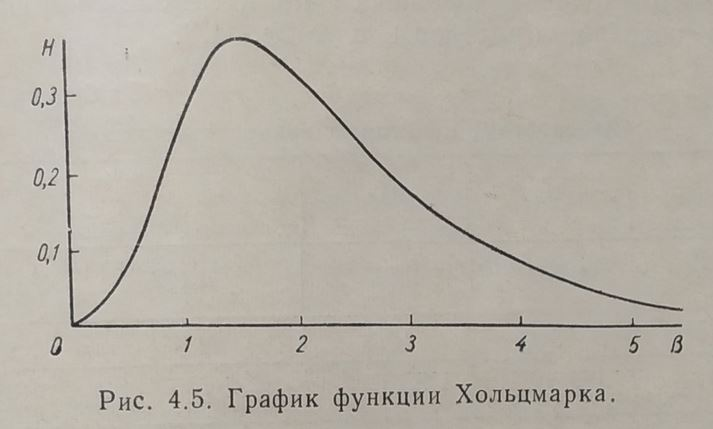
\includegraphics[width=0.6\linewidth]{Holsmark.JPG}
	\end{center}
\end{figure}

Стоит сказать про \uline{функцию распределения}. Под действием столкновений плазма максвеллизируется~\cite{kroll} [здесь -- нормированная на концентрацию]:

\begin{equation}
	f(v) = \sqrt{\left( \frac{m}{2\pi T}\right)^3} e^{-\frac{mv^2}{2T}}
\end{equation}

или

\begin{equation}
	f(E) = \frac{2\pi}{\sqrt{\left(\pi T\right)^3}}\sqrt{E} e^{-\frac{E}{T}}
\end{equation}

\uline{Идеальная и неидеальная плазма}. Вводят либо число частиц в дебаевской сфере (сфера с радиусом $\lambda_D$) $N = \frac{4\pi}{3}n\lambda_D^3$, либо обратный ему параметр неидеальности $g = \frac{1}{n\lambda_D^3}$~\cite{kroll}. Случай $g \ll 1$: плазма идеальна, число частиц в деб. сфере большое, энергия взаимодействия много меньше кинетической энергии частиц плазмы (коллективные эффекты $\gg$ одночастичные; кулоновским взаимодействием часто можно пренебречь). В этом случае её свойства, как газа, схожи с идеальным газом -- никакие две частицы этого газа заряженных частиц не взаимодействуют (поэтому <<идеальная>>).

Важно: $g \sim \frac{n^{1/2}}{T^{3/2}}$, стремление к нулю соответствует <<разряженной>> плазме. Отсюда следует другой вид критерия идеальности: $T \gg e^2 n^{1/3}$~\cite{kotelnikov}.

Важно: в идеальном газе взаимодействует МАЛО частиц, в идеальной плазме взаимодействуют МНОГО частиц (но очень слабо).

Покажем, как энергия взаимодействия связана с числом частиц в дебаевской сфере. Рассмотрим точечный заряд $q$ в плазме. Его потенциал в плазме из-за экранировки равен $\varphi = q/r\exp{-r/\lambda_D}$, однако в вакууме он равен $\varphi_{vac}=q/r$. Это значит, что разницу между $\varphi$ и $\varphi_{vac}$ cоздали все частицы плазмы, окружающие этот точечный заряд.
Значит, что энергия взаимодействия (электростатическая) точечного заряда со всеми остальными частица плазмы равна $q (\varphi - \varphi_{vac})$, где потенциал плазмы надо рассчитывать в точке нахождения точечного заряда, т.е. в точке $r=0$. В итоге получаем энергию взаимодействия $-q^2/\lambda_D$.
Видно, что эта энергия в общем случае отличается от оценки кулоновского взаимодействия $q^2/\langle r\rangle$, где $\langle r \rangle = n_e^{-1/3}$~---~среднее расстояние между частицами.

В случае, когда плазма действительно ведёт себя как плазма, а не газ, и экранирует заряды, отношение потенциальной энергии к кинетической рассчитывается следующим образом:

\begin{equation}
	\frac{W}{T} \approx \frac{e^2}{\lambda_D T} = \frac{8\pi n e^2}{T}\frac{1}{8\pi n\lambda_D} = \frac{1}{8\pi n \lambda_D^3}
\end{equation}

Заметим, что это отношение с точностью до численного множителя равно обратному числу частиц в дебаевской сфере. Таким образом, если плазма идеальная и число частиц в дебаевской сфере большое, то кинетическая энергия частиц (тепловая) много больше их потенциального взаимодействия, как в идеальном газе. Однако в обычном газе потенциальную энергию надо учитывать без экранировки и критерий идеальности действительно получается другим, а именно:

\begin{equation}
	\frac{W}{T} \approx \frac{e^2}{\langle r \rangle T} = \frac{e^2 n^{1/3}}{T} \ll 1
\end{equation}

\subsection{Условие термодинамического равновесия, термическая ионизация, формула Саха, корональное равновесие, снижение потенциала ионизации}

Следующий параграф посвящён рассмотрению процессов ионизации и рекомбинации в общем виде и поиску равновесия/математического описания подобных плазменных процессов.

\uline{Термическая ионизация} -- ионизация, при которой необходимую энергию для отрыва электрона от атома дают столкновения между атомами вследствие повышения температуры.

\uline{Условие термодинамического равновесия}. Плазма -- открытая система (т.к. излучает, вылетает, ...). Работает принцип детального равновесия: скорости прямого (ионизация) и обратного (рекомбинация) процессов должны в нём быть равны.

\begin{itemize}

\item Рассмотрим следующую пару процессов: ионизация электронным ударом $\leftrightarrow$ рекомбинация при тройных столкновениях~\cite{frank}.

Их скорости: $w_{ion} = k_{ion}n_an_e$ и $w_{rec} = k_{rec}n_in_e^2$ соответственно. $w_{ion}$ и $w_{rec}$ -- функции только температуры. Равновесие [закон действующих масс~\cite{frank}]:
 
\begin{equation} \label{eq:detailed_balance}
	K = \frac{k_{ion}}{k_{rec}} = \frac{n_in_e}{n_a},
\end{equation}

где $K$ -- константа равновесия. 

\item Рассмотрим следующую пару процессов: ионизация излучением $\leftrightarrow$ рекомбинация при двойных столкновениях с излучнием~\cite{frank}.

Их скорости: $w_{ion, rad} = k_{ion, rad}n_aI$ и $w_{rec, rad} = k_{rec, rad}n_in_e$ соответственно. $w_{ion}$ и $w_{rec}$ -- функции только температуры. Равновесие:

\begin{equation}
	\frac{k_{ion, rad}I}{k_{rec, rad}} = \frac{n_in_e}{n_a}.
\end{equation} 

\end{itemize}

Следовательно, общий вид условия термодинамического равновесия ионизации:

\begin{equation}
	K = \frac{k_{ion}}{k_{rec}} = \frac{k_{ion, rad}I}{k_{rec, rad}} = \frac{n_in_e}{n_a}
\end{equation}

Важно: если плазма всё-таки закрытая система, то условие выполняется автоматически. Если открытая, то может реализоваться ситуация, что ионизация и рекомбинация идут по разным путям (электронным ударом и с излучением соответственно). 

В таком случае балансное уравнение на концентрацию электронов имеет следующий простой вид:

\begin{equation}
	\pdv{n_e}{t} = k_{\text{ион}}n_en_a-k_{\text{рек}}n_en_i,
\end{equation}

откуда следует, что равновесная [стационарная] концентрация электронов и ионов определяется формулой Эльверта:

\begin{equation}
	\alpha = n_i/n_a = k_{\text{ион}}/k_{\text{рек}}
\end{equation}

Это выражение называется также \uline{корональным равновесием}~\cite{kotelnikov}, т.к. реализуется в солнечной короне. 

Важно: степень ионизации не зависит от плотности плазмы.

Для равновесной ионизации [термодинамически равновесной плазмы], однако, существует фундаментальное \uline{уравнение Саха}, описывающее степень ионизации плазмы как функции температуры, давления и энергии ионизации атомов.

Условия применимости: ионизация и рекомбинация проходят по одному и тому же пути, плазма рассматривается как идеальный газ (при не слишком низких и не слишком высоких плотностях), кулоновская энергия мала по сравнению с тепловой [идеальная плазма]. 

Вывод~\cite{frank}:

Число электронов с импульсом от $\vec{p}$ до $\vec{p}+\vec{dp}$ в объёме $V$:

\begin{equation*}
	\dd N_e = \dd\Gamma(p)/V_{el} \cdot P(\varepsilon) = 4\pi p^2 V\dd p\cdot \frac{1}{h^3} \cdot g_e e^{-\frac{\varepsilon}{T}},
\end{equation*}

где $\dd\Gamma(p)$ -- объём фазового пространства для частицы с импульсом от $\vec{p}$ до $\vec{p}+\vec{dp}$ ; $V_{el} = h^3$ -- элементарный объём фазового пространства; $P(\varepsilon)$ -- вероятность наличия частицы с заданной энергией. Здесь $g_e$ -- статистический вес, т. е. число состояний с одинаковой энергией, различающихся внутренними степенями свободы. $\varepsilon = I_p + \frac{p^2}{2m}$, где $I_p$ -- потенциал ионизации. Тогда число свободных электронов на один атом в определенном
квантовом состоянии:

\begin{equation*}
	N_e^{*} = \int\limits_{0}^{\infty} \dd N_e = Vg_e\frac{(2\pi mT)^{3/2}}{h^3}e^{-\frac{I_p}{T}}
\end{equation*}

Полное число электронов получается умножением на число атомов в одном квантовом состоянии и заменой $V$ на объём, приходящийся на число ионов в определённом квантовом состоянии ($1/\frac{n_i}{g_i}$):

\begin{equation*}
	N_e = N_e^{*} \cdot N_a/g_a = \frac{g_i}{n_i} g_e\frac{(2\pi mT)^{3/2}}{h^3}e^{-\frac{I_p}{T}} \cdot \frac{N_a}{g_a}
\end{equation*}

Отсюда следует, что

\begin{equation} \label{eq:Saha}
	\frac{n_en_i}{n_a} = \frac{N_en_i}{N_a} = \frac{g_eg_i}{g_a} \frac{(2\pi mT)^{3/2}}{h^3}e^{-\frac{I_p}{T}}
\end{equation}

Классический вид уравнения Саха -- это как раз выражение~\eqref{eq:Saha}. Часто, однако, оно записывается для случая многоступенчатой ионизации:

\begin{equation*}
	\frac{n_en_{i+1}}{n_i} = \frac{g_eg_{i+1}}{g_i} \frac{(2\pi mT)^{3/2}}{h^3}e^{-\frac{I_p^{(i)}}{T}}
\end{equation*}

Применимость: [астрофизика] Равновесная ионизация, описываемая уравнением Саха, объясняет эволюцию в ранней Вселенной. После Большого взрыва все атомы были ионизированы, оставив в основном протоны и электроны. Согласно подходу Саха, когда Вселенная расширилась и остыла так, что температура достигла примерно 3000 К, электроны рекомбинировали с протонами, образуя атомы водорода. В этот момент Вселенная стала прозрачной для большей части электромагнитного излучения. При исходной температуре $T = 3000 K$ с красным смещением примерно 1000 отсюда следует реликтовое излучение с $T = 3 K$, которое пронизывает всю Вселенную сегодня. 

Орбита сильно возбуждённого электрона далеко удалена от ядра, и на него влияют другие частицы. Электроны, окружающие атом, всё сильнее экранируют поле ядра, и когда радиус электронной орбиты превышает масштаб экранирования, сила притяжения атомного электрона к ядру начинает падать с расстоянием по экспоненциальному закону В таком при $r>\lambda_D$ связанные состояния не реализуются, и электрон становится свободным при энергии возбуждения, меньшей потенциала ионизации изолированного атома. Происходит как бы \uline{снижение потенциала ионизации}. Главное квантовое число $n$ последнего возбуждённого состояния можно оценить из условия $n^2a_0 \sim \lambda_D$ или $n \sim 10^4\sqrt{\lambda_D(\text{см})}$.

\subsection{Вырождение плазмы, статистика Больцмана и Ферми—Дирака, модель Томаса—Ферми}

\uline{Вырожденная [квантованная] плазма}: $T \leq \varepsilon_F$, где $\varepsilon_F$ -- энергия Ферми [максимально возможная энергия для фермиона при $T=0$]. Невырожденная плазма/описываемая классической физикой: $T \gg \varepsilon_F$. [Вырожденная = т.к. кв. состояния электронов вырождены по энергии, на каждом уровне их по два].

Новым эффектом в вырожденной плазме является обменное взаимодействие, не имеющее аналога в классической физике~\cite{kotelnikov}.

Важно: до экстремально низких температур ионы -- классические.

Слегка другой подход по\Tokman: плотность частиц в фазовом объёме в классическом случае: $\left( \frac{1}{\Delta p^3}\right)_{classic} = \frac{N}{p_T^3} = \frac{N}{m^3v_T^3}$; в квантовом: $\left(\frac{1}{\Delta p^3}\right)_{quantum} = \frac{V}{2 \pi \hbar^3}$ [следует из периодичности г.у. для рассматриваемого объёма]. Как правило, $\left( \frac{1}{\Delta p^3}\right)_{classic} \ll \left(\frac{1}{\Delta p^3}\right)_{quantum}$. Когда за счёт $N\uparrow$ достигает равенства, то надо учитывать квантовые эффекты и статистика Максвелла-Больцмана $\rightarrow$ статистика Ферми-Дирака. Условие классической статистики: $\frac{mv_T}{\hbar} = \lambda_D^{-1} \gg n^{1/3}$ ($\lambda_D$~---~длина волны де Бройля)

\uline{Распределение Больцмана} описывает распределение частиц в условиях термодинамического равновесия идеальной невырожденной плазмы:

\begin{equation}
	n = n_0e^{-\frac{\varepsilon}{T}}
\end{equation}

\uline{Распределение Ферми-Дирака} используется для описания вырожденной плазмы:

\begin{equation}
	f(\varepsilon) = \frac{1}{e^{\frac{\varepsilon-\varepsilon_F}{T}}+1}
\end{equation}

В пределе $T\rightarrow 0$ с вероятностью 1 заняты низшие состояния с энергией $\varepsilon \leq \varepsilon_F$; при $T \gg \varepsilon_F$ и $\varepsilon \gg \varepsilon_F$ распределение Ферми—Дирака переходит в распределение Больцмана.

Квантовые эффекты проявляются тогда, когда расстояние между частицами соразмерно с длиной волны де Бройля, то есть когда волновые функции частиц соприкасаются, но не перекрываются. [Вики]

Можно описывать плазму с помощью квантовомеханической \uline{модели Томаса-Ферми} в случаях, когда не работает модель Саха (вырожденная плазма; неидеальная плазма, большое число ионов)~\cite{kalitkin}. Можно даже сказать, что обобщенная модель Саха описывает газовую плазму, а модель Томаса-Ферми -- жидкую плазму. \sout{Переход между этими состояниями выше критической точки не является фазовым, а происходит плавно.}

\section{Элементарные процессы}

Часто для описания плазмы используют разбиение процессов на соударения и пролёт между соударениями. Такой подход, строго говоря, не применим для соударения заряженных частиц. При этом самыми вероятными (= важными) являются парные столкновения\Tokman. 

\subsection{Столкновения заряженных частиц, дальнодействие, частоты столкновений, столкновения электронов с атомами (упругие и неупругие), столкновения тяжёлых частиц. [Терминология]}

Соударения делятся на:
\begin{itemize}
	\item неупругие/неупругие первого рода -- возбуждение -- суммарная поступательная энергия частиц уменьшается;
	\item упругие [внутреннее состояние не меняется, обмен поступательной энергией] -- поступательная энергия частиц не меняется;
	\item сверхупругие/неупругие второго рода -- девозбуждение -- поступательная энергия частиц увеличивается~\cite{raizer}.
\end{itemize}

Как правило, упругие столкновения электрон испытывает намного чаще, чем неупругие. Поэтому для проводимости и поглощательной способности ионизированного газа, а также для диффузии электронов важнейшую роль играют именно упругие столкновения~\cite{raizer}.

Основные термины: длина свободного пробега [см], среднее время между соударениями [с], частота столкновений [Гц], эффективное сечение процессов [см$^2$]. 

Дифференциальные термины: дифференциальное сечение (рассеяния) [см$^2$].

Интегральные термины: транспортное сечение [см$^2$] и эффективная частота столкновений [Гц].

\subsubsection{Основные термины}

\uline{Эффективное сечение}. Согласно~\cite{raizer}: $\sigma(v) = \frac{\nu}{nv}$, где $\nu$ -- число соударений в секунду [частота]; $n$ -- плотность налетающих частиц; $v$ -- скорость налетающих частиц. Для газокинетических столкновений его можно оценить как $\sigma \approx \pi(r_1+r_2)^2$, где $r_1$ и $r_2$ -- характерные радиусы частиц. Согласно~\cite{astap}: $\sigma=\int\limits_{0}^{\infty} 2\pi \rho P(\rho) d\rho$, где $\rho$ -- прицельный параметр, $P(\rho)$ -- вероятность рассеяния (зависит от конкретных реагентов). 

\uline{Частота столкновений}: $\nu = n\left\langle v\sigma(v)\right\rangle $. В случае максвеллизации в газе из молекул одного сорта: $\nu = \sqrt{2}n\overline{v}\pi d^2$. 
Если рассматривается сразу несколько процессов, например, разные сорта газа или возбуждение нескольких уровней, то

\begin{equation*}
	\nu = \sum_{i}n_i\overline{v}\sigma_i
\end{equation*}

\uline{Среднее время между соударениями}: $\tau = 1/\nu$.

\uline{Длина свободного пробега}: $l = 1/(n\sigma)$.
Для разных сортов газа или рассмотрения нескольких процессов:

\begin{equation*}
	\frac{1}{l} = \sum_{i}\frac{1}{l_i}\approx\sum_{i}n_i\sigma_i
\end{equation*}

\subsubsection{Дифференциальные и интегральные термины}

Для ввода остальных терминов надо более подробно рассмотреть случай парного столкновения.	

\begin{quotation}
	Важно: Совершенно необязательно рассматривать в классической плазме взаимодействие в классическом виде. Та же ионизация -- квантовый процесс (хоть может быть описана и в классическом виде тоже)\Tokman.
\end{quotation}

{\bfseries \large I. Частоты столкновений.} Рассмотрим два сорта частиц $\alpha$ и $\beta$ ($e, i, n$) и перейдём в систему центра масс:

\begin{figure}[ht]
	\begin{center}
		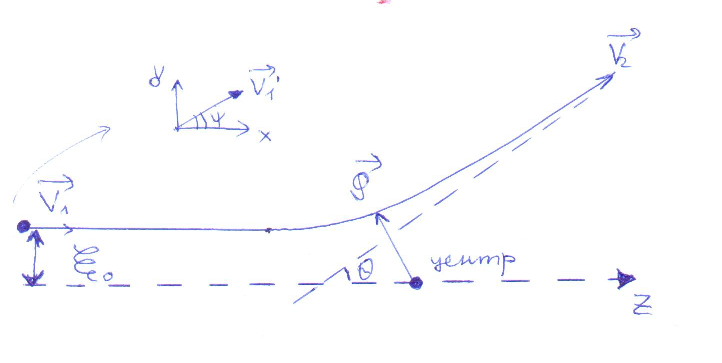
\includegraphics[width=0.6\linewidth]{scattering_simple.pdf}
	\end{center}
	\caption{Рисунок из лекций}
	\label{fig:scattering}
\end{figure}

\begin{equation} \label{eq:center_mass}
	\vec{R} = \frac{m_\alpha\vec{r_\alpha}+m_\beta\vec{r_\beta}}{m_\alpha+m_\beta}
\end{equation}

\begin{equation*}
	\vec{\rho} = \vec{r_\alpha}-\vec{r_\beta};\,
	\vec{V} = \dot{\vec{R}};\,
	\vec{v} = \dot{\vec{\rho}}
\end{equation*}

Можно показать, что кинетическая энергия равна

\begin{equation*}
	K = m_\Sigma\frac{V^2}{2}+\mu_{\alpha\beta}\frac{v^2}{2},
\end{equation*}

где $\mu_{\alpha\beta}$ -- приведённая масса. 

Гамильтониан:

\begin{equation*}
	H = \frac{p^2}{2\mu_{\alpha\beta}}+U(\abs{\vec{\rho}});\,
	\vec{p} = \mu_{\alpha\beta}\vec{v}
\end{equation*}

Также надо учесть законы сохранения: 1. Поскольку рассматривается упругое рассеяние: $U(\pm \infty) = 0, v_1 = v_2 = 0$ 2. Сохранение момента импульса (система замкнута): $\vec{L} = \vec{\rho} \times \vec{p} = \vec{\rho} \mu_{\alpha\beta} \vec{v} = const$.

Более-менее строгий вывод:

\begin{equation*}
	\Delta p_\alpha = \mu_{\alpha\beta} \Delta v_\alpha
\end{equation*}

\begin{equation*}
	\Delta v_\alpha = \Delta v_{\alpha_{z}} = -(1-cos\theta)v
\end{equation*}

Тогда

\begin{equation} \label{eq:center_mass_K}
	\Delta K_\alpha = \mu_{\alpha\beta}\vec{V}\overrightarrow{\Delta p_\alpha} 
\end{equation}

В силу симметрии можно записать:

\begin{equation*}
	\theta = \pi - 2 \int\limits_{\rho_{min}}^{\infty}\frac{\xi_0 \dd r}{\rho\sqrt{1-\frac{\xi_0^2}{\rho^2}-\frac{U(\rho)}{K_0}}}
\end{equation*}

Таким образом, результат [если не требуется точная зависимость]: $\theta = \theta(v, \xi_0)$.

{\bfseries \large II. Столкновения электронов с атомами [упругие].} Перейдём от парного столкновения к рассмотрению рассеивающего поток частиц центра. Цель: определить среднее число частиц $dN'$, улетающих в единицу времени в элемент телесного угла при заданных $\theta$ и $\psi$.

Очевидно, что $\dv{N'}{t} \sim nv;\, \dv{N'}{t} \sim \dd \Omega$. Введём коэффициент пропорциональности, имеющий размерность площади:

\begin{equation*}
	\dv{N'}{t} = \dd\Omega\cdot nv \cdot \sigma_{\alpha\beta}(\theta, v)
\end{equation*}

Так как в процессе столкновения число частиц не изменяется, то число частиц, которое после рассеяния попадает в элемент телесного угла $d\Omega$, равно числу частиц, которые налетают на рассеивающий центр с прицельным параметром $\xi_0$, т.е.:

\begin{equation*}
	\dv{N'}{t} = \dd S \cdot nv = \xi_0 d\xi_0 \dd\psi   \cdot nv
\end{equation*}

Приравнивая, получаем:

\begin{equation*}
	\sigma_{\alpha\beta} \dd\Omega = \sigma_{\alpha\beta} sin\theta \cdot \dd\theta \cdot \dd\psi = \dd\psi \cdot \xi_0 \cdot \dd\xi_0
\end{equation*}

Тогда (добавляем модуль из соображений того, что ранее писали без учёта знаков):

\begin{equation} \label{eq:transport_cs}
	\sigma_{\alpha\beta} = \frac{\xi_0}{sin\theta}\abs{\dv{\xi_0}{\theta}}
\end{equation}
где $\dd\xi_0/\dd\theta$ надо понимать в смысле $(\dd\theta/\dd\xi_0)^{-1}$, т.к. при решении задачи мы обычно ищем зависимость угла рассеяния от прицельного параметра, а не наоборот.

$\sigma_{\alpha\beta}$ называется \uline{диффференциальным сечением рассеяния} и имеет смысл той площади, с которой частицы летят в определённый угол.

Дифференциальное сечение важно, поскольку в эксперименте положение детектора соответствует какому-то телесному углу и нужен пересчёт измеренных данных в физические характеристики процесса.

Полное сечение рассеяние определяется как интеграл от дифференциального сечения по всем телесным углам:

\begin{equation} \label{eq:total_cs}
	S_{\alpha\beta} = \int \sigma_{\alpha\beta} \dd\Omega = 2 \pi \int_{0}^{\pi} \sigma_{\alpha\beta} sin\theta \cdot \dd\theta
\end{equation}

Полное число частиц сорта $\alpha$, сталкивающихся в единицу времени в единице объёма с частицами сорта $\beta$, равно

\begin{equation*}
	\dv{n_\alpha}{t} = n_\alpha n_\beta S_{\alpha\beta} v = n_\alpha\nu_{\alpha\beta},
\end{equation*}

где $\nu_{\alpha\beta}$ -- частота столкновений = полное число столкновений частицЫ сорта $\alpha$ с частицами сорта $\beta$ в единицу времени.

Изменение импульса в единицу времени в единице объёма:

\begin{equation*}
	\left\langle \Delta \vec{p_\alpha}\right\rangle = \left\langle -\mu_{\alpha\beta}(1-cos\theta)v \right\rangle = -\mu_{\alpha\beta}n_\alpha n_\beta \int \dd^3v v \vec{v} S_{\alpha\beta}^t(v) = -\mu_{\alpha\beta}n_\alpha\int \dd^3v \vec{v}\nu_{\alpha\beta}^t,
\end{equation*}

где $S_{\alpha\beta}^t(v)$ -- тот же интеграл $S_{\alpha\beta}$ из~\eqref{eq:total_cs}, но с весом $1-cos\theta$ (аналогично с $\nu_{\alpha\beta}^t$). Эти величины называются \uline{транспортными}\Tokman.

\begin{quotation}

Другой подход\cite{raizer}: \uline{Транспортным сечением} реакции называется выражение $\sigma_{tr} = \sigma_c(1-\langle {cos\theta}\rangle$, где $\sigma_c$ -- полное сечение рассеяния, а $\theta$ -- угол между конечной и начальной скоростью рассеянной частицы. Выражение $\nu_m = nv\sigma_{tr}$ носит название \uline{эффективной частоты столкновений}. Ей соответствует длина пробега $l_m = 1/(n\sigma_{tr})$. При изотропном рассеянии эти величины совпадают с полными сечением, частотой и длиной пробега. При ситуации, когда в основном рассеяние происходит ``вперёд'' (т.е. скорость налетающей частицы после взаимодействия направлена практически в ту же сторону), транспортное сечение и эффективная частота столкновений меньше истинных. Если рассеяние происходит ``назад'', то -- больше. Таким образом, данные величины введены для индикации отличия рассеяния от изотропного.

Считая тяжёлые частицы (атомы, молекулы, ионы) неподвижными, можно показать~\cite{raizer}, что потери энергии $\delta_\varepsilon = \frac{2m}{M}(1-\langle cos\theta\rangle)$, что при переходе к ``эффективным'' соударениям даёт долю потерянной энергии в одном эффективном взаимодействии в $\frac{2m}{M}$. 

Важно: это очень малая величина, поэтому температура электронов (которые, \uline{как правило}, греются) и ионов сильно отличаются/долго выравниваются.

\end{quotation}

Изменение энергии в единицу времени в единице объёма:

\begin{equation*}
	\left \langle \Delta K_\alpha \right \rangle = - \varkappa_{\alpha\beta} (1-cos\theta) (K_\alpha-K_\beta),
\end{equation*}

где $\varkappa_{\alpha\beta} = \frac{2m_\alpha m_\beta}{(m_\alpha+m_\beta)^2}$.

Если мы хотим использовать величины, иллюстрирующие множество процессов, то в выражениях, например, для транспортного сечения надо добавить $\sum$ и перейти к $\Delta E_j$. 

Важно: Рассеяние на атоме можно считать классической задачей, если: $\lambda_\text{де Бройля} = \frac{\hbar}{m_\alpha v_T} \ll r_{min} \sim a_{Bohr} = \frac{\hbar^2}{m_e e^2}$, что соответствует $K_e \gg I$ [потенциала ионизации] -- тогда задача классическая. В случае ионизации работает классика, если передаётся энергии более чем $I$ [отсюда тоже можно взять оценку\Tokman].

Важно: у некоторых атомов и молекул наблюдаются глубокие минимумы сечений в области энергий $\varepsilon \sim 0.1-1$ эВ --- \uline{эффект Рамзауэра} \cite{raizer} (принципиально квантовый), аналогичный эффекту пятна Пуассона в оптике. Роль ``экрана'' для электрона играет атом. Если длина волны де Бройля электрона сравнима с размером атома, то в результате дифракции электрона за атомом возникает максимум электронной волны — электрон ``огибает'' атом без рассеяния на нём.

По факту, заполненная внешняя оболочка атома внутри себя создаёт квантовую яму с резкими стенками. Электрон - можно рассматривать как волну. При некоторых обстоятельствах волна может интерферировать с этой ямой. 

\begin{quotation}
	
	Точное решение квантово-механической задачи рассеяния электрона на атоме дает следующее выражение для транспортного сечения упругого рассеяния:
	
	\begin{equation*}
		\sigma_{tr}^{quantum} = 4\pi \left(L^{2}+\frac{4}{5}\frac{\pi \alpha L}{a_{Bohr}}\frac{m_ev}{\hbar}+\frac{\pi^{2}}{6}\frac{\alpha^{2}}{a_{Bohr}^{2}}\left( \frac{m_ev}{\hbar}\right) ^{2} \right), 
	\end{equation*}
	
	где $L$ -- т.н. ``длина рассеяния''; $\alpha$ -- поляризуемость атома [входит в потенциал взаимодействия].
	
	Слагаемые соответствуют: короткодействующему взаимодействию (1), дальнодействующему потенциалу (3) и интерференции двух этих эффектов [проявляются волновые свойства электрона; может быть отрицательным].
	
	\begin{itemize}
		\item[$\oplus$] И. Мак-Даниэль ``Процессы столкновений в ионизированных газах'', гл. 3, \S 15.
	\end{itemize}
	
\end{quotation}

{\bfseries \large III. Столкновения заряженных частиц. Дальнодействие.} Рассмотрим парные кулоновские столкновения.

Берём из термеха \uline{формулу Резерфорда}:

\begin{equation} \label{eq:Rutherford}
	\xi_0 = r_s ctg\frac{\theta}{2},
\end{equation}

где $r_s = \frac{e^2}{\mu_{\alpha\beta}v_\infty^2}$ -- называется кулоновским радиусом (при нём потенциальная энергия взаимодействия сравнима с кинетической энергией относительного движения, а лёгкая частица отклоняется в результате взаимодействия на угол $\theta=\frac{\pi}{2}$\cite{raizer}). Тогда из~\eqref{eq:transport_cs}:

\begin{equation*}
	\sigma_{\alpha\beta} = \frac{\xi_0}{\sin\theta}\abs{\dv{\xi_0}{\theta}} = r_s^2\frac{\cos\frac{\theta}{2}}{2\sin^2\frac{\theta}{2}\cos\frac{\theta}{2}}\frac{1}{2\sin^2\frac{\theta}{2}} = \frac{r_s^2}{4\sin^4\frac{\theta}{2}}
\end{equation*}

В таком случае~\eqref{eq:total_cs}:

\begin{equation*}
	S_{\alpha\beta}^t = 2\pi\int\limits_{\theta_{min}}^{\pi}\frac{r_s^2}{4\sin^4\frac{\theta}{2}}\sin\theta(1-\cos\theta)\dd\theta = 2\pi r_s^2\int\limits_{\theta_{min}}^{\pi} \frac{\cos\frac{\theta}{2}}{\sin\frac{\theta}{2}}\dd\theta = -4\pi r_s^2 \cdot \ln\left( \sin\frac{\theta_{min}}{2}\right) 
\end{equation*}

Проблема: бесконечно сильное столкновение (само по себе нефизично) + потенциально отсутствие распространения волн в плазме (опровергается экспериментом).

Расходится в области малых углов $\theta_{min}\sim\xi_{max}$, где $K\gg U$. Проведём аппроксимацию:

\begin{equation*}
	\sin\frac{\theta_{min}}{2}\approx \frac{\theta_{min}}{2} = \frac{1}{\left[ 1+\left( \frac{\xi_0^{max}}{r_s}\right)^2 \right]^{1/2}} \approx \frac{r_s}{\xi_0^{max}} \approx \frac{r_s}{\lambda_D}
\end{equation*}

Итак, 

\begin{equation*}
	S_{\alpha\beta}^t = 4\pi r_s^2 \cdot \ln\frac{\lambda_D}{r_s} = 4\pi r_s^2 L,
\end{equation*}

где $L$ -- \uline{кулоновский логарифм} (порядок величины: 15-17 в токамаке, обычно берут равным 10). Основной вклад в сечение дают рассеяния на малые углы. В этом и проявляется \uline{дальнодействие}: малые углы $\sim$ большие прицельные параметры. Важно: здесь не была учтена разница между средними скоростями электронов и ионов.

Кулоновский логарифм:

\begin{equation*}
	L = \ln\frac{\lambda_D}{r_s} \sim \ln\frac{(T/(ne^2))^{1/2}}{e^2/T} = \ln\frac{T^{3/2}}{n^{1/2}e^3}
\end{equation*}

\begin{equation} \label{eq:Coulomb_log}
	L_e = 23+\frac{3}{2}\ln(T_e)-\frac{1}{2}\ln(n); L_i = 23+
	\frac{3}{2}\ln(T_{i,e})-\frac{1}{2}\ln(n)
\end{equation}

$T_{i,e} = min(T_e, T_i)$, [$T$] = эВ, [$n$] = см$^{-3}$.

Частоты столкновений:

\begin{equation} \label{eq:freq_ee}
	\nu_{ee}^t = \frac{16\pi e^4 n}{m_e^2v_e^3}L_{ee},
\end{equation}

$v_e\sim v_T$ -- тепловая.

\begin{equation} \label{eq:freq_ei}
	\nu_{ei}^t = \frac{\nu_{ee}^t}{4},
\end{equation}

т.к. приведённая масса в два раза больше.

\begin{equation} \label{eq:freq_ii}
	\nu_{ii}^t = \frac{16\pi e^4 n}{m_i^2v_i^3}L_{ii}
\end{equation}

\begin{equation*}
	\nu_{ei} = \frac{4\pi e^4 n}{m^2v^3}L_{ee} \approx \frac{\omega_{pe}^4}{nv_{Te}^3}L_{ee} = \frac{\omega_{pe}}{n\lambda_D^3}L_{ee}
\end{equation*}

Условие идеальной плазмы: $n\lambda_D^3 \gg 1$, то $\nu_{ei} \ll \omega_{pe}$. $\nu_{ei}$ определяет коэффициент затухания плазменных колебаний.

Дополнение: В квантовой механике нет предельного параметра -- кажется, что нет и дифференциального сечения рассеяния. Однако в ней возможен такой же подход с разделением/заменой переменных, но уже в уравнении Шрёдингера (на движение ц. масс и относительно него). 

Знание сечений элементарных процессов (в т.ч. -- из квантовой механики) позволяет полностью описать систему в рамках данного подхода.

\subsection{Неупругие столкновения электронов с атомами. Ионизация, рекомбинация, перезарядка и прилипание. Возбуждение и диссоциация молекул электронным ударом}

\subsubsection{Ионизация}

\begin{equation}
	A + e \rightarrow A^{+} + 2e
\end{equation}

\uline{Потенциал ионизации} $I$ -- энергия связи электрона в атоме (ионе), которую необходимо затратить, чтобы эту связь разорвать. Соответственно, процесс ионизации носит пороговый характер. Вблизи $\varepsilon \approx I$ сечение ионизации можно аппроксимировать как: $\sigma = C(\varepsilon-I)$. Характерное сечение ионизации $[C\times1 \text{эВ}]$ см$^2$, соответствующее $\varepsilon = I + 1\text{эВ}$, на два порядка
меньше сечений упругих соударений электронов. В максимуме сечение ионизации обычно в два или несколько раз меньше упругого при той же энергии~\cite{raizer}.

Для ионизации существует формула Томсона, которая выводится из классических соображений (разумеется, является достаточно грубым приближением). 

%Рассматривается упругое соударение двух электронов: налетающего и ``связанного'' с атомом. Налетающий передаёт второму электрону энергию $\Delta\varepsilon$ (ионизация в данном случае определяется как случай $\Delta\varepsilon > I$). Тогда из~\eqref{eq:center_mass_K}:
%
%\begin{equation*}
%	\Delta \varepsilon = \mu \vec{V}\vec{v} (1-\cos\theta) = \frac{m_e}{2} \frac{v_1^2+v_2^2}{2} (1-\cos\theta) = \frac{\varepsilon}{2} (1-\cos\theta)
%\end{equation*}
%
%и из~\eqref{eq:total_cs} и~\eqref{eq:Rutherford}:
%
%\begin{equation*}
%	\sigma_{ion}^{Th} = 2\pi\int\frac{r_s^2}{4\sin^4\frac{\theta}{2}}\sin\theta d\theta = \frac{\pi r_s^2}{2} \int\frac{4}{(1-\cos\theta)^2}d(\cos\theta) = 2\pi r_s^2\int_{I}^{\varepsilon}\frac{\varepsilon^2}{4\Delta\varepsilon^2}\frac{-2\Delta\varepsilon}{\varepsilon} = \frac{\pi e^4}{4\varepsilon^2}\frac{\varepsilon-I}{I}
%\end{equation*}
%
%[как-то возникла лишняя четвёрка -- не думаю, что это критично для экзамена, но в книгах в знаменателе её нет]

Очевидно, что $\sin\theta = p_\perp/p$, где $p_\perp$ и $p$ -- поперечный и полный импульсы после рассеяния. Рассеяние упругое: $p = p_0 = \sqrt{2\mu\varepsilon}=\sqrt{2\frac{m_em_a}{m_a}\varepsilon} = \sqrt{2m_e\varepsilon}$ (здесь $\varepsilon$ -- энергия свободного электрона). Очевидно, что рассеивающий центр (связанный электрон в данном случае) приобретает такой же импульс по 3-му закону Ньютона, тогда энергия изначально связанного электрона после рассеяния $\varepsilon_b=p_\perp^2/2m$. Тогда

\begin{equation*}
	\sin\theta = \frac{p_\perp}{p} = \sqrt{\frac{\varepsilon_b}{\varepsilon}} = 
	\frac{e^2}{\varepsilon\xi_0}\Rightarrow 
	\xi_0^2 = \frac{e^4}{\varepsilon \varepsilon_b}
\end{equation*}

Дифференциальное сечение рассеяния имеет вид:

\begin{equation*}
	\dd\sigma = 2\pi\xi_0\dd\xi_0 = \pi \dd\xi_0^2 = \pi\frac{e^2}{\varepsilon\varepsilon_b^2}\dd\varepsilon_b
\end{equation*}

Полное сечение:

\begin{equation}
	\sigma = \frac{\pi e^2}{\varepsilon}\int\limits_{I}^\varepsilon\frac{\dd \varepsilon_b}{\varepsilon_b^2} = \frac{\pi e^2}{\varepsilon}\left( \frac{1}{I} - \frac{1}{\varepsilon} \right) = \frac{\pi e^2}{\varepsilon^2}\frac{\varepsilon - I}{I}
\end{equation}

Для большей точности формулу представляют часто в виде~\cite{astap}:

\begin{equation*}
	\sigma_{ion}^{Th} = \pi a_I^2 f^{Th}(\varepsilon/I),
\end{equation*}

где $a_I = \frac{e^2}{I}$ -- радиус ионизации = расстояние, на котором энергия кулоновского взаимодействия равна потенциалу ионизации; $f^{Th}(x) = \frac{x-1}{x^2}$ -- безразмерная функция Томсона. Грубая оценка: $\sigma_{ion} = \pi a_I^2$. Т.к. энергия входит в виде $\varepsilon/I$, используются методы подобия, когда в каждом отдельном случае определяется вид функции $f^{Th}(x)$. 

Важно: для расчёта ионизации многоэлектронных атомов электронным ударом будет сумма таких выражений с весом в виде функции Хэвисайда (пороговость процесса).

Процесс ионизации в плазме осуществляется в основном электронами с энергией, заметно превосходящей температуру плазмы [т.н. ``хвост'' максвелловского распределения]~\cite{astap}. Поэтому ионизация становится заметной уже при температурах, достаточно малых по сравнению с потенциалами ионизации атомом (например, при $T=1$ эВ в водородной плазме с $I_p=13.6$ эВ).

Кроме того, может происходить \uline{многоступенчатая ионизация} -- т.е. ионизация через возбуждённые уровни, в несколько этапов. Такой процесс возможен для электронов с энергией меньше, чем потенциал ионизации. Сечение ионизации возбуждённого атома существенно выше, чем невозбуждённого. 

Можно рассматривать и ионизацию ионов. Очевидно, что для неё сечение процесса меньше, чем для атома (влияние положительного атомного остатка)~\cite{raizer}.

\subsubsection{Рекомбинация} \label{subsubsec:recombination}

\begin{equation}
	A^{+Z} + e + C \rightarrow A^{+(Z-1)} + C',
\end{equation}

где через $C$ и $C'$ обозначено состояние третьего тела (наличие которого необходимо для выполнения ЗСЭ) до и после реакции. Важно, что в качестве $C$ может выступать даже электронный остов рекомбинирующего иона~\cite{astap}. Может в результате излучать фотон -- фото-/радиационная рекомбинация.

Плотная холодная плазма (большой радиус кулоновского взаимодействия): доминирует трёхчастичная рекомбинация, разреженная горячая плазма: фоторекомбинация.

В результате баланса между ионизацией и рекомбинацией в плазме устанавливается ионизационное равновесие, характеризуемое определенным соотношением между концентрацией нейтральных и заряженных частиц, а также между концентрацией
ионов с различными зарядами. 

\uline{Трехчастичная рекомбинация} является процессом, детально обратным процессу ионизации:

\begin{equation*}
	A^{+Z} + 2e \rightarrow A^{+(Z-1)} + e 
\end{equation*}

Для вывода скорости рекомбинации через детальный баланс~\eqref{eq:detailed_balance} и см., например, ~\cite{astap}), нужно использовать формулу Саха~\eqref{eq:Saha} и знать вид выражения для константы скорости соответствующей ионизации.

Используя их, можно показать, что скорости прямой и ступенчатой ионизации соотносятся как

\begin{equation}
	\frac{k_{\text{прям}}}{k_{\text{ступ}}} \approx \left(\frac{T}{I}\right)^{\frac{7}{2}}
\end{equation}

\uline{Диэлектронная рекомбинация} является наряду с трехчастичной и радиационной одним из основных процессов образования ионов меньшей кратности в плазме с достаточно низкой плотностью, где преобладают процессы парных соударений. Для реализации этого вида рекомбинации необходимо наличие у рекомбинирующего иона некоторого числа остаточных электронов, т.е. электронного остова, который берёт на себя избыток энергии рекомбинирующего электрона~\cite{astap, raizer}.

\begin{equation*}
	A^{+Z} + e \leftrightarrow A^{**}
\end{equation*}

Диэлектронная рекомбинация преобладает над трехчастичной рекомбинацией в достаточно разреженной плазме (малые $n_e$) и при достаточно высокой температуре плазмы.

\uline{Диссоциативная рекомбинация} состоит из двух этапов. Первый: объединение молекулярного иона $AB^{+}$ и электрона в квазимолекулу, которая находится в сверхвозбужденном автоионизационном состоянии. Второй: переход в молекулу $AB$ (может и не существовать: инертные газы) или в два атома $A$ и $B$; один из них может быть и возбужденным. Это возможно, если потенциальная кривая какого-либо из состояний системы атомов $A^{*}+B$ пересекает потенциальную кривую иона $AB^{+}$.

\begin{equation*}
	AB^{+} + e \leftrightarrow A^{*}+B \rightarrow AB | A+B
\end{equation*}

Системы $AB^{+}+e$ и $A^{*}+B$ при междуядерном расстоянии около $r_m$ имеют одинаковые энергии (см. рис. \ref{fig:diss_recomb}). Поэтому возможен самопроизвольный переход из первой конфигурации во вторую. 

\begin{figure}[ht]
	\begin{center}
		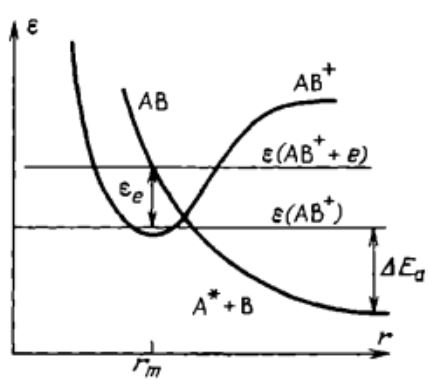
\includegraphics[width=0.3\linewidth]{diss_recomb.jpg}
	\end{center}
	\caption{Схема потенциальных кривых для случая диссоциативной рекомбинации}
	\label{fig:diss_recomb}
\end{figure}

Коэффициент диссоциативной рекомбинации равен:

\begin{equation}
	\beta_{\text{дисс\textunderscore рекомб}} = k_{\text{захв}}\frac{\omega_{\text{стаб}}}{\omega_{\text{стаб}}+\omega_{\text{авто}}} = \frac{k_{\text{захв}}}{\omega_{\text{авто}}}\frac{\omega_{\text{стаб}}\omega_{\text{\text{авто}}}}{\omega_{\text{стаб}}+\omega_{\text{авто}}},
\end{equation}

где $\omega_{\text{стаб}}$ -- вероятность стабилизации [c$^{-1}$] (обратное время жизни состояния); $\omega_{\text{авто}}$ -- вероятность автоионизации; $k_{\text{захв}}$ -- константа скорости захватов.

$\omega_{\text{стаб}} \sim v_a/a$ -- отношение скорости разлёта атомов квазимолекулы к их характерному размеру. $\omega_{\text{стаб}} \sim 10^{14}$ c$^{-1}$ -- очень быстрый процесс (для сравнения скорость высвечивания кванта $v_{q} \sim 10^{8}$ c$^{-1}$).

\subsubsection{Перезарядка}

Столкновения заряженных тяжелых частиц с атомами и молекулами зависит от состояний сталкивающихся частиц. Столкновения ионов с атомами в низкотемпературной плазме относятся к типу медленных столкновений, которые характеризуются особенностями квазимолекулы, образованной сталкивающимися ионом и атомом~\cite{astap}.

Важным условием для взаимодействия тяжёлых частиц [но не только их] является условие быстроты воздействия~\cite{astap}. Грубо говоря, при медленном столкновении атома с частицей плазмы электронные оболочки атома успевают за время столкновения подстроиться под движение налетающей частицы и затем вернуться в исходное положение после окончания столкновения. Говорят, что частицы движутся по адиабатическим молекулярным термам, не переходя в другие атомные состояния. Таким образом, условием служит малость отношения частоты к частоте пролета возмущающей частицы: 

\begin{equation} \label{eq:Messi}
	M = \frac{\rho \omega}{v} \ll 1,
\end{equation}

$\rho$ -- прицельный параметр, $v$ -- относительная скорость, $\omega$ -- частота перехода.

Обратное условие, отвечающее малости вероятности перехода при медленном столкновении, называется адиабатическим критерием Месси, а сам параметр $M$, входящий в условие~\eqref{eq:Messi} -- \uline{параметром Месси}.

Можно рассмотреть простейший случай -- двухуровневую квазимолекулу (см. рис. \ref{fig:terms_quasimol}). Общее решение, однако, при произвольных скоростях изменения потенциалов
взаимодействия невозможно получить в аналитическом виде. Приближённое решение можно получить с использованием борновского приближения. Борновское приближение расходится при малых прицельных параметрах пролета. В результате получается
функция, описывающая плавный переход от борновского предела
к экспоненциальному спаду, содержащему в экспоненте параметр Месси (характерные изменения в виде переходов в зависимости от скорости процесса -- см. рис. \ref{fig:transitions_2levels}).

\begin{figure}[h]
	\begin{center}
		\begin{minipage}[h]{0.49\linewidth}
			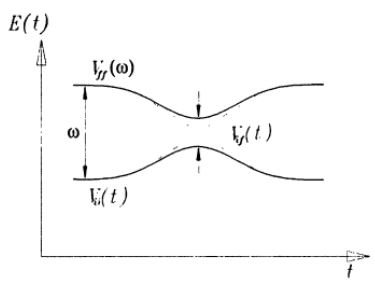
\includegraphics[width=1\linewidth]{heavy_particle.jpg}
			\caption{Эволюция во времени термов квазимолекулы, образованной сталкивающимися тяжёлыми частицами} 
			\label{fig:terms_quasimol}
		\end{minipage}
		\hfill
		\begin{minipage}[h]{0.49\linewidth}
			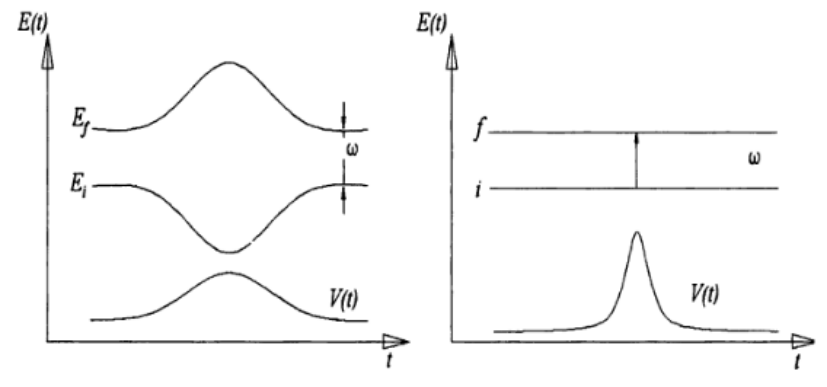
\includegraphics[width=1\linewidth]{2levels_transition.png}
			\caption{Схема переходов в двухуровневой системе при медленных (слева) и быстрых (справа) столкновениях. Внизу показано изменение возмущений во времени}
			\label{fig:transitions_2levels}
		\end{minipage}
	\end{center}
\end{figure}

\uline{Резонансная перезарядка} состоит в передаче электрона от одного ядра к другому в системе идентичных ядер.

\begin{equation*}
	A + A^{+} \rightarrow A^{+} + A
\end{equation*}

Что изменилось: произошёл обмен скоростями между нейтральным атомом и ионом (хотя направления движения каждой частицы останется прежним).

Взаимодействие атома и иона определяется перекрытием волновых функций двух ядер, т.е. фактически при перезарядке электрон туннелирует между двумя потенциальными ямами (см. рис.~\ref{fig:charge_exchange}). При уменьшении относительной скорости $v$ вероятность электрона находиться в потенциальной яме каждого из ядер стремится к $1/2$~\cite{astap}.

\begin{figure}[ht]
	\begin{center}
		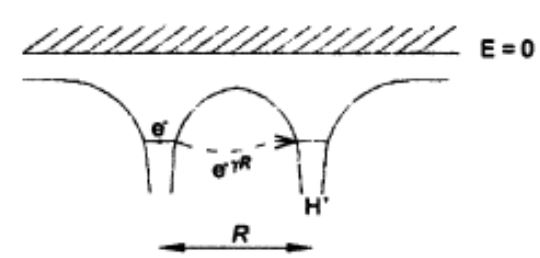
\includegraphics[width=0.5\linewidth]{res_recharge.jpg}
	\end{center}
	\caption{Схема туннелирования атомного электрона (внизу) при резонансной перезарядке}
	\label{fig:charge_exchange}
\end{figure}

\uline{Нерезонансная перезарядка} состоит в передаче электрона от одного ядра к другому в случае неидентичных ядер с разными энергиями связи электрона на каждом из них.

Особый случай соответствует перезарядке атома на многозарядном ионе, потенциал ионизации которого намного превосходит потенциал ионизации исходного атома. Здесь атомный электрон переходит в густой спектр высоковозбужденных состояний многозарядного иона, для которых энергия связи близка к энергии связи в исходном атоме. Сечение такой перезарядки $\sigma_{exchange} \sim Zn^4$, где $Z$ -- заряд иона, $n$ -- номер орбиты~\cite{astap}.

\subsubsection{Прилипание}

Процесс прилипания дополнительного электрона к изначально нейтральным атомам или молекулам достаточно важен. Например, это канал потерь электронов, который может быть использован. Большие потери электронов в газах с активными электроотрицательными [свойство притягивать к себе дополнительные электроны] добавками затрудняют развитие в них электронной лавины, что повышает напряжение пробоя. Это используют в счётчиках Гейгера, в которых быстрые ядерные и атомные частицы регистрируются благодаря производимой ими ионизации. После пролета частицы необходимо возможно скорее устранить электроны, чтобы подготовить прибор для регистрации нового разрядного импульса.
 
Механизмы прилипания электронов к нейтральным частицам во многом похожи на механизмы рекомбинации электронов с положительными ионами: фотозахват, тройные столкновения, диссоциативное прилипание.
 
Термодинамически равновесные плотности отрицательных ионов не зависят от механизмов образования и разрушения ионов и определяются уравнением Саха, в котором по смыслу роль положительных ионов играют нейтральные частицы, а роль атомов и молекул — отрицательные ионы.

\uline{Прилипание в результате фотозахвата.} Захват электронов атомами водорода с испусканием кванта имеет важное значение в излучении звезд, но практически неважен в исследовании газового разряда.

\uline{Прилипание в результате тройных столкновений.} Затрат энергии для этого процесса не требуется, и потому он легко идет при комнатной температуре электронов и в очень слабых полях. Малые (но не чрезмерно) энергии электронов для него даже предпочтительнее. В некоторых газах, в частности -- в воздухе, прилипание в тройных столкновениях является главным механизмом потерь медленных электронов.

\begin{equation*}
	e + A + A \leftrightarrow A^{-} + A
\end{equation*}

Фактически подобные процессы протекают многоступенчатым путем. Например, для воздуха электрон вначале в парном столкновении захватывается молекулой $O_2$ в автоионизационное состояние. При этом сверхвозбужденными оказываются не электронные степени свободы, как при безызлучательном захвате электрона положительным ионом, а молекулярные колебания. В последующих соударениях с молекулами сверхвозбужденные ионы, которые не успели совершить автоионизационный распад, стабилизируются благодаря ударной дезактивации (``тушению''). Иногда столкновения вызываются действием поляризационных сил, и молекула просто отбирает у иона часть колебательной энергии: иногда наряду с передачей энергии происходит резонансная перезарядка. С молекулами кислорода последний вариант случается даже чаще.

\uline{Диссоциативное прилипание.} По данному механизму образовываются в плазменном объёме отрицательные ионы водорода. Для них он происходит в две стадии: сначала ``горячий'' электрон ($\varepsilon \approx 30-100$ эВ) возбуждает высокие колебательные состояния молекулы водорода, а потом к ней прилипает холодный ($\varepsilon \sim 1$ эв) электрон, квазимолекула распадется на искомый ион $H^{-}$ и атом $H$.

Процессы диссоциативного прилипания имеют резонансный характер. В зависимости от энергии электрона наблюдаются резко выраженные максимумы сечений~\cite{raizer}. При повышении температуры газа сечение диссоциативного прилипания возрастает, а энергетический порог реакций понижается, но так происходит лишь после некоторого повышения температуры.

\subsubsection{Возбуждение и диссоциация молекул электронным ударом}

\uline{Возбуждение в результате соударения с электроном.} Три основных типа атомно-молекулярных частот: электронные с энергиями порядка нескольких эВ, колебательные с энергиями порядка долей эВ, вращательные с энергиями порядка сотых долей эВ~\cite{astap}.

Возбуждения \uline{электронных состояний} существенным образом влияют на скорость развития электронной лавины во многих случаях пробоя газов. Они составляют первый этап процесса ступенчатой ионизации в газе и вообще являются главным механизмом появления возбужденных атомов и молекул в плазме. Возбуждение атомов и молекул в значительной степени обусловливает свечение разрядной плазмы~\cite{raizer}.

В отличие от ударной ионизации, когда атомный электрон возбуждается в непрерывный энергетический спектр, соответствующий инфинитному движению, в случае возбуждения атомный электрон переходит в состояние дискретного спектра, то есть (в рамках классической картины) на другую атомную орбиту с большей энергией. Это явление ответственно за излучение фотонов в плазме, возникающее в результате обратного перехода атомного электрона из возбужденного состояния в основное~\cite{astap}.

\begin{equation*}
	e + A \rightarrow A^{*} + e
\end{equation*}

Атом при взаимодействии с электромагнитным полем ведёт себя как набор осцилляторов, которые ставятся в соответствие паре энергетических уровней $E_i$ и $E_j$ атомного спектра причём собственные частоты этих осцилляторов равны собственной частоте перехода $\omega_{i,j}=\frac{E_j-E_i}{\hbar}$ (для дипольно-разрешённых переходов).

Дипольно-запрещённые переходы бывают двух типов: без изменения спина атома (дипольный момент перехода отсутствует из-за невыполнения правил отбора по орбитальному квантовому числу $L$, переход осуществляется за счёт прямого кулоновского взаимодействия) и переходы с изменением атомного спина (в этом случае возбуждение атома происходит за счет обменного взаимодействия между налетающим и атомным электроном)~\cite{astap}.

Среди возбужденных атомов и молекул выделяются метастабильные частицы. Из метастабильных состояний запрещен, т. е. имеет чрезвычайно малую вероятность, самопроизвольный переход в нижнее энергетическое состояние, сопровождающийся излучением кванта. Следовательно, в таких состояниях частица может жить долго, до тех пор, пока она не дезактивируется ударом другой частицы, электрона или атома и не перейдетв более высокое состояние или не ионизируется. В сильно разреженных газах это время может быть весьма большим. Времена жизни метастабильных состояний по отношению к высвечиванию превышают $10^{-4}$ с и достигают в некоторых случаях секунд, тогда как обычные возбужденные атомы и молекулы высвечиваются через $10^{-9}-10^{-7}$ с (если не будут до этого дезактивированы ударом). Особенно велика роль метастабильных частиц для процесса ступенчатой ионизации, так как они живут долго и поэтому ``с легкостью ожидают'' ионизирующего удара.

Самый нижний из неметастабильных уровней называют резонансным. Возможен такой процесс: атом излучает квант света, возвращаясь в основное состояние. Этот квант с большой вероятностью поглощается соседним атомом, поскольку происходит резонансное поглощение, и переводит его на тот же самый резонансный уровень. Второй атом излучает квант и т. д. Так происходят блуждание (диффузия) резонансного излучения и периодическое появление и исчезновение резонансно возбужденных атомов. Процессу препятствует дезактивация (тушение) резонансно возбужденных атомов.

Эффективное сечение возбуждения электронного состояния $\sigma_{exc}(\varepsilon)$ называют иногда функцией возбуждения. В зависимости от энергии электрона это сечение ведет себя в качественном отношении так же, как сечение ионизации, только максимум располагается ближе к порогу. Этот процесс -- сугубо квантовый. С ростом энергии спадает как $ln(\varepsilon)/\varepsilon$, имеет максимум при $\varepsilon=3.45 \Delta \varepsilon$.

Возбуждение \uline{колебательных частот} играет существенную роль в разрядах, происходящих в молекулярных газах, будучи главным механизмом передачи энергии от электронов молекулам. Можно провести аналогию с ударами по двум шарам, соединённых пружиной. Иногда процесс идёт через промежуточное состояние (отрицательный молекулярный ион).

При рассмотрении возбуждения \uline{вращательных частот} можно провести аналогию с ударами по гантели (два жёстко соединённые шара). Вообще говоря, роль возбуждения и дезактивации молекулярных вращений электронным ударом для разрядных процессов не очень существенна. В атомарных газах этого процесса просто нет, а в молекулярных обмен вращательной энергией значительно уступает обмену колебательной, так как соответствующие порции энергии -- колебательные кванты -- на несколько порядков больше~\cite{raizer}.

\uline{Диссоциация молекул в результате соударения с электроном.} Удары достаточно энергичных электронов могут приводить и к диссоциации молекул. Этот неупругий процесс, как правило, не оказывает существенного влияния на энергетический баланс электронов в разряде, уступая в этом отношении возбуждению колебательных уровней молекул. Но в определенных условиях диссоциация молекул имеет большое непосредственное значение, будучи начальным этапом в цепочке последующих химических превращений. Для многих плазмохимических реакций ``узким местом'', определяющим скорость всего процесса, является образование из молекул атомов и свободных радикалов, которые потом уже достаточно быстро реагируют с другими компонентами. Прохождению этого этапа и способствует диссоциация молекул ударами электронов в разряде. Вероятность прямого разбиения молекулы за счет кинетической энергии электрона очень мала. Диссоциация идет двухступенчатым путем, но в отличие от возбуждения колебаний не через захват электрона, а через возбуждение электронных или электронно-колебательных состояний молекулы с последующим распадом возбужденной молекулы на атомы. Вклад в диссоциацию дает возбуждение нескольких подходящих уровней молекулы, соответствующих нестабильным состояниям, так что процесс идет по нескольким каналам. Процесс носит пороговый характер, порог определяется не потенциалом диссоциации, а потенциалом возбуждения низшего нестабильного электронного состояния~\cite{raizer}.

\section{Физическая кинетика}
\label{sec.3}

Макроскопические уравнения плазмы являются уравнениями переноса в том смысле, что они описывают поток импульса, энергии и т. д. Однако термин «явления переноса» употребляется в физике плазмы обычно для обозначения свойств плазмы, связанных со столкновительными эффектами, т. е. таких свойств, как электропроводность, теплопроводность, диффузия частиц поперек или вдоль магнитного поля и т. д. Во многих плазменных задачах поведение плазмы определяется влиянием нейтральных атомов или молекул. Например, диффузия электронов в редкой низкотемпературной частично ионизованной плазме определяется главным образом столкновениями электронов с нейтралами. Кроме того, разнообразные процессы в плазме происходят в результате ионизации при столкновениях и электрон-ионной рекомбинации. В проблеме явлений переноса в плазме имеются два аспекта. Первый из них связан с вычислением различных коэффициентов переноса на основании соответствующего статистического описания и анализа механизмов, приводящих к этим явлениям. Другой аспект состоит в том, чтобы с помощью полученных коэффициентов рассчитать ожидаемую макроскопическую картину поведения плазмы при данных начальных и граничных условиях~\cite{kroll}.

\subsection{Уравнения Больцмана и Власова, интеграл столкновений, время максвеллизации и скорость выравнивания температур различных компонент плазмы}

Наиболее подробное описание плазмы дается набором изменяющихся во времени координат и скоростей всех частиц. Для реальной плазмы достичь такого уровня описания невозможно. Предлагается использовать формализм теории вероятностей и статистической физики\Tokman.

Поскольку в течение промежутков времени, меньших времени электрон-ионных столкновений, поведение электронов и ионов может сильно различаться, обычно необходимо определять для частиц каждого сорта $\alpha$ свою функцию распределения $f_\alpha(\vec{r_\alpha}, \vec{v_\alpha})$.

\subsubsection{Ввод понятия функции распределения}

Рассмотрим ящик классических частиц объёмом $V$, в котором $N$ частиц: $\vec{r_1}, \vec{r_1},\ldots,\vec{r_N}$. 

Тогда плотность вероятности найти первую частицу в $\vec{r_1}$, вторую -- в $\vec{r_2}$ и т.д. [без учёта движения частиц=скорости] вводится как $\omega(\vec{r_1}, \vec{r_1},\ldots,\vec{r_N})$ (нормирована на единицу: $\prod\limits_{j} \int\limits_{V} \dd^3r_j \omega = 1$).

Число частиц в объёме $\Delta V$ вводится как интеграл от $n(\vec{r})=\sum\limits_{j}\delta(\vec{r}-\vec{r_j})$ -- концентрации:

\begin{equation*}
	\Delta N = \int\limits_{\Delta V} n(\vec{r}) \dd^3r,
\end{equation*}

Введём для концентрации выражение через усреднение по вероятностному распределению:

\begin{equation*}
	n(\vec{r}) = \prod\limits_{j}\int\limits_{V}\dd^3r_j \sum\limits_{j} \delta(\vec{r}-\vec{r_j})\omega(\vec{r_1}, \vec{r_2}, \vec{r_N}) = \sum\limits_j \omega_{1j}(\vec{r})\delta(\vec{r}-\vec{r_j}),
\end{equation*}

где $\omega_1(\vec{r_j}) = \prod\limits_{j'\neq j}\omega(\vec{r_1} \ldots \vec{r_j} \ldots \vec{r_N}) d^3r_{j'}$ -- вероятность найти первую [если одинаковые: одну] частицу в $\vec{r_j}$.

Для случая одинаковых частиц (т.е. частиц одного сорта) $\omega_1$ -- одинаковые. Тогда $n(\vec{r}) = N\cdot\omega_1(\vec{r})$.

\begin{quotation}
	[Оффтоп] Вероятность нахождения первой из одинаковых частиц в $\vec{r}$, а второй -- в $\vec{r'}$: $\omega_2(\vec{r}, \vec{r'}) = \omega_1(\vec{r})\omega_{1}(\vec{r'})$.
\end{quotation}

Рассмотрим 2 сорта частиц $\alpha$ и $\beta$. Для них плотность вероятности вводится так: \newline $\omega_{\alpha\beta}(\overrightarrow{r_{1\alpha}}\ldots\overrightarrow{r_{N\alpha}},\overrightarrow{r_{1\beta}}\ldots\overrightarrow{r_{N\beta}})$, причём вероятность найти одну частицу сорта $\alpha$ в заданной точке $\omega_{1\alpha}$ получается интегрированием по всем $\vec{r_\beta}$ и по всем $\vec{r_\alpha}$, кроме одной.

Введём плотность вероятности с учётом того, что частицы движутся: $\overrightarrow{r_{\alpha, \beta}}\Rightarrow\overrightarrow{r_{\alpha, \beta}};\overrightarrow{v_{\alpha, \beta}}$ (полный набор координат частицы описывает её нахождение в 6D пространстве координат/скоростей). Теперь имеет смысл оперировать понятием вероятности найти одну частицу в заданной точке с заданной скоростью $\omega_{1\alpha}(\overrightarrow{r_\alpha}, \overrightarrow{v_\alpha})$.

\uline{Функция распределения} [ФР; часто используется сокращение ФРЭЭ -- функция распределения электронов по энергиям] частиц сорта $\alpha$ [по скоростям и координатам] вводится так:

\begin{equation} \label{eq:distribution_func}
	f_\alpha(\overrightarrow{r_\alpha}, \overrightarrow{v_\alpha}) = n_\alpha\cdot\omega_{1\alpha}(\overrightarrow{r_\alpha}, \overrightarrow{v_\alpha})
\end{equation}

[Физ. смысл] ФР есть плотность частиц в фазовом пространстве. Интеграл от неё по скоростям есть концентрация частиц, по скоростям и координатам -- полное число частиц выбранного сорта~\cite{kotelnikov}.

\subsubsection{Вычисление макрохарактеристик плазмы с использованием ФР}

Концентрация частиц:

\begin{equation*}
	n_\alpha(\vec{r}) = \int\limits_{\infty}f_\alpha \dd^3v_\alpha
\end{equation*}

Средний поток частиц:

\begin{equation*}
	\Pi_\alpha(\vec{r}) =	\int\limits_{\infty}\overrightarrow{v_\alpha}f_\alpha \dd^3v_\alpha
\end{equation*}

Средний импульс:

\begin{equation*}
	p_\alpha(\vec{r}) = \int\limits_{\infty}m_\alpha\overrightarrow{v_\alpha}f_\alpha \dd^3v_\alpha
\end{equation*}

Средняя кинетическая энергия:

\begin{equation*}
	K_\alpha(\vec{r}) = \int\limits_{\infty}\frac{m_\alpha\overrightarrow{v_\alpha}}{2}f_\alpha \dd^3v_\alpha \xrightarrow{\text{если не зависит от $\vec{r}$}} \left\langle K_\alpha\right\rangle n_\alpha
\end{equation*}

\subsubsection{Двухчастичная ФР}

Собственно, имеет вид $f_{\alpha\beta}(\overrightarrow{r_\alpha}, \overrightarrow{r_\beta}, \overrightarrow{v_\alpha}, \overrightarrow{v_\beta}) = n_\alpha n_\beta \widetilde{f_{\alpha\beta}}(\overrightarrow{v_\alpha}, \overrightarrow{v_\beta})$. Для независимых (невзаимодействующих)

\begin{equation} \label{eq:Boltzmann_relation}
	f_{\alpha\beta} = f_\alpha f_\beta
\end{equation}

\begin{quotation}
	Последнее выражение -- \uline{приближение Больцмана}\Tokman. Если написать последовательно кинетические уравнения для $N, N-1, \ldots, 1$-частичных функций распределения, получится т.н. цепочка уравнений Боголюбова. Это приближение позволяет её замкнуть и решить. 
\end{quotation}
	
\begin{equation*}
	\int\limits_{\infty}f_{\alpha\beta}(\overrightarrow{r_\alpha}, \overrightarrow{r_\beta}, \overrightarrow{v_\alpha}, \overrightarrow{r_\beta})\dd^3v_\alpha \dd^3v_\beta = n_{\alpha\beta}(\overrightarrow{r_\alpha}, \overrightarrow{r_\beta}) \xrightarrow{\text{независимые}} n(\overrightarrow{r_\alpha}) n(\overrightarrow{r_\beta})
\end{equation*}
	
Разница $n_{\alpha\beta}-n_\alpha n_\beta$ перестаёт быть малой на радиусе корреляции (дебаевский радиус), однако в первом приближении ФР расщепляется.

\subsubsection{Вывод уравнения Больцмана}

Рассмотрим частицы одного сорта $f(\vec{r}, \vec{v}, t)$ при наличии внешней силы $\vec{F}(\vec{r}, t)$, где $\vec{r} = \vec{r}(t)$, $\vec{v} = \vec{v}(t)$.
	
У системы уравнений движения есть два векторных интеграла движения, сохраняющихся на решениях уравнений: $\vec{r_0} = \vec{r_0}(t, \vec{v}, \vec{r})$; $\vec{v_0} = \vec{v_0}(t, \vec{v}, \vec{r})$ В начальный момент было $f(\overrightarrow{r_0}, \overrightarrow{v_0})$. Значит, [т.к. нормировка = общее число частиц сохраняется]: 

\begin{equation*}
	f(\vec{r}, \vec{v}, t) = f(\overrightarrow{r_0}(t, \vec{v}, \vec{r}), \overrightarrow{v_0}(t, \vec{v}, \vec{r})) \cdot \abs{\frac{D(\vec{r}, \vec{v})}{D(\overrightarrow{v_0}, \overrightarrow{r_0})}} = f(\overrightarrow{r_0}(t, \vec{v}, \vec{r}), \overrightarrow{v_0}(t, \vec{v}, \vec{r})) \cdot J
\end{equation*}
	
Мы рассматриваем частицы под воздействием полей, а столкновения и трения не рассматриваем, то система консервативная и по теореме Лиувилля якобиан $J=1$. 
$f(\overrightarrow{r_0}(t, \vec{v}, \vec{r}), \overrightarrow{v_0}(t, \vec{v}, \vec{r}))$ -- интеграл движения как функция от интегралов; значит, $f(\vec{r}, \vec{v}, t)$ -- тоже.

Значит, \uline{кинетическое уравнение в бесстолкновительном приближении}/\newline\uline{бесстолкновительное уравнение Больцмана}/\uline{уравнение Лиувилля}

\begin{equation} \label{eq:Liouville_eq}
	\dv{f}{t} = \pdv{f}{t} + \dv{\vec{r}}{t}\pdv{f}{\vec{r}}+ \frac{\vec{F}}{m}\pdv{f}{\vec{v}} = 0
\end{equation}

Важно: здесь $F$ -- сила не трения, а подобная силе Лоренца, чтобы работала теорема Лиувилля.

Если в системе есть соударения, то справа надо дописать ещё столкновительный член $St$ (он же -- \uline{интеграл столкновений}, оператор соударений, часто обозначается как $\pdv{f}{t}\bigg|_\text{столк}$). Строгий вывод: последовательное интегрирование уравнений Лиувилля (цепочка уравнений Боголюбова). Интеграл столкновений по физическому смыслу есть скорость изменения функции распределения в результате столкновений. Больцмановский подход предполагает рассмотрение только парных столкновений и замыкание системы (см. выше приближение Больцмана~\eqref{eq:Boltzmann_relation}).

\uline{Уравнение Больцмана}:

\begin{equation} \label{eq:Boltzmann_eq}
	\dv{f}{t} = \pdv{f}{t} + \dv{\vec{r}}{t}\pdv{f}{\vec{r}}+ \frac{\vec{F}}{m}\pdv{f}{\vec{v}} = St
\end{equation}

Важно: Фазовое пятно из-за столкновений не сохраняется.

Важно: Хотя кинетическое уравнение Больцмана не дает точного описания эволюции распределения в результате столкновений в полностью ионизованной плазме, его можно использовать для вычисления коэффициентов переноса
в слабоионизованной плазме, где превалируют упругие столкновения электронов с нейтральными частицами~\cite{kroll}.

Свойства: 1. При интегрировании кинетического уравнения по скорости получаем:

\begin{equation*}
	\pdv{n}{t} + div(n\vec{v}) = \int\limits_{\infty}\dd^3v\cdot St
\end{equation*}

Из уравнения непрерывности следует, что для любого интеграла столкновений 

\begin{equation*}
	\int\limits_{\infty}\dd^3v\cdot St = 0
\end{equation*}

2. При равновесной $f=f_0$ интеграл столкновений зануляется: $St = 0$
	
\subsubsection{Время максвеллизации и скорость выравнивания температур различных компонент плазмы} \label{subsec: maxwellization_time}

Существуют разные подходы к конкретному виду интеграла столкновений. Стоит точно назвать интегралы соударений в формах Больцмана, Фоккера-Планка и БГК. Более подробно они рассмотрены в первом билете дополнительной программы~\eqref{subsec:collision_terms}.

Существует приближение, связанное с введением времени свободного пробега (т.н. $\tau$-приближение, а уравнение Больцмана с ним называется модифицированным). В этом методе больцмановский интеграл столкновений заменяют следующим выражением~\cite{kroll}:

\begin{equation*}
	\pdv{f}{t}\bigg|_\text{столк} = \frac{f_0-f(\vec{r}, \vec{v}, t)}{\tau(v)}\approx-\frac{f_0-f(\vec{r}, \vec{v}, t)}{\tau},
\end{equation*}

где $\tau$ -- постоянное время свободного пробега. Уравнение Больцмана в таком виде иногда называют \uline{моделью Крука}.

Данный подход отражает представление о том, что любое распределение
релаксирует к равновесному распределению $f_{\alpha 0}$ за счет столкновений и что существует некоторое характерное время (в общем случае зависящее от скорости) между столкновениями с передачей импульса -- \uline{время максвеллизации}.

Применимость:

1. [Закон сохранения числа частиц] Равновесная функция $f_0$ имеет вид распределения Максвелла-Больцмана:

\begin{equation*}
	f_{\alpha 0} = \frac{n_\alpha(\vec{x}, t)}{\overline{n_\alpha}} \left( \frac{m_\alpha}{2\pi \varkappa T_\alpha}\right)^{3/2}e^{-m_\alpha v^2/(2\varkappa T_\alpha)}, 
\end{equation*}

\begin{equation*}
	\frac{n_\alpha(\vec{x}, t)}{\overline{n_\alpha}} \equiv \int f_\alpha (\vec{r}, \vec{v}, t) \dd\vec{v},
\end{equation*}

где $\overline{n_\alpha}$ -- отношение полного числа частиц к полному объёму системы.

2. Интеграл столкновений видоизменяет распределение таким
образом, что средняя скорость обращается в нуль. Это удачное приближение для столкновений электронов с нейтральными частицами, а, значит, слабоионизованной плазмы. Подобный подход называется моделью Лоренца.

Замена $\tau(v)$ на $\tau$ является точной в случае короткодействующей силы. Выбор времени т, не зависящего от функции распределения $f_\alpha$, который линеаризует больцмановский интеграл
столкновений, возможен только тогда, когда отсутствуют столкновения
между частицами того же распределения.

3. Член $\frac{f}{\tau}$ описывает уход частиц, распределенных согласно
$f(\vec{r}, \vec{v}, t)$, за счет рассеяния из элемента $d\vec{v}$. Это напоминает процесс поглощения, поскольку все частицы, первоначально находившиеся в элементе $d\vec{v}$, исчезают из данного элемента после рассеяния. Второй член интеграла столкновений описывает приход частиц в элемент $d\vec{v}$ за счет рассеяния;
ему трудно найти аналогию в исходном уравнении Больцмана. Форма $\frac{f_0}{\tau}$ предполагает, что после каждого столкновения испускаются частицы с максвелловским распределением и локальной плотностью $n(\vec{r}, t)$.

\uline{Скорость выравнивания температур различных компонент в плазме}

\subsubsection{Уравнение Власова} \label{subsubsec:Vlasov_eq}

Случай бесстолкновительной плазмы во внешних э/м полях:

\begin{equation} \label{eq:Vlasov_eq_main}
	\pdv{f_\alpha}{t}+\vec{v}\pdv{f_\alpha}{\vec{r}}+e_\alpha\left(\vec{E}+
	\frac{1}{c}\left[\vec{v}\times\vec{B}\right]\right)\pdv{f_\alpha}{\vec{p}}=0
\end{equation}

При рассмотрении плазмы в э/м полях возникают сложности при использовании больцмановского подхода~\eqref{eq:Boltzmann_eq}, а именно: рассматриваются только парные столкновения, сечения которых при кулоновском взаимодействии, строго говоря, расходятся, т.к. оно имеет дальнодействующий характер и одна частица взаимодействует не с одной, а с совокупностью частиц. Соответственно и то эффективное поле, которым можно описать
это взаимодействие, создаётся большим числом частиц, т. е. имеет
макроскопический характер. Тем самым весь процесс приобретает
макроскопически достоверный, а не случайный характер. Есть и другие причины (см, например, [Вики],~\cite{kotelnikov}).

Этому случайному характеру формально отвечает представление точных
микроскопических значений электрического и магнитного полей, действующих на некоторую частицу в плазме, в виде~\cite{kotelnikov}:

\begin{align*}
	\vec{E} = \langle\vec{E}\rangle+\vec{e};\\
	\vec{B} = \langle\vec{B}\rangle+\vec{b},	
\end{align*}

где $\langle\vec{E}\rangle$ и $\langle\vec{B}\rangle$ -- некие средние поля, создаваемые ``средней'' плотностью заряда и ``средним'' током в плазме, а микрополя $\vec{e}$ и $\vec{b}$ представляют собой мелкомасштабные флуктуации полей, отвечающие
столкновениям частиц. Переобозначим $\langle\vec{E}\rangle$ и $\langle\vec{B}\rangle$ как $\vec{E}$ и $\vec{B}$. Условие на них -- уравнения Максвелла:

\begin{align} \label{eq:Vlasov_eq_Maxwell}
	rot\vec{E} = -\frac{1}{c}\pdv{\vec{B}}{t},\;div\vec{B}=0;\\
	rot\vec{B} = \frac{1}{c}\pdv{\vec{E}}{t} + \frac{4\pi}{c}\vec{j},\;div\vec{E}=4\pi\rho;
\end{align}

где плотности заряда и тока выражаются через саму ФР:

\begin{align} \label{eq:Vlasov_eq_extra}
	\rho = \sum\limits_{\alpha}\int e_\alpha f_\alpha \dd^3p, \\
	\vec{j} = \sum\limits_{\alpha}\int e_\alpha \vec{v}f_\alpha \dd^3p;
\end{align}

Самосогласованная система уравнений~\eqref{eq:Vlasov_eq_main}, ~\eqref{eq:Vlasov_eq_Maxwell},~\eqref{eq:Vlasov_eq_extra} с т.н. самосогласованными полями $\vec{E}$ и $\vec{B}$ -- уравнения Власова (или просто~\eqref{eq:Vlasov_eq_main} -- \uline{уравнение Власова}).

\subsection{Явления переноса в плазме, электропроводность, диффузия и теплопроводность частиц при наличии и отсутствии магнитного поля} \label{subsec:transport_phenomena}

Эволюция плазмы заключается в направлении выравнивания её параметров между различными частями пространства за счёт процессов переноса, которые приводят к перераспределению плотности, импульса и энергии между различными областями плазмы. Процессами переноса называют в совокупности диффузию, теплопроводность и вязкость. В замкнутой системе они ведут к установлению полного термодинамического равновесия. Они обусловлены кулоновскими столкновениями, но идут ещё медленнее, нежели локальное выравнивание температуры ионов и электронов~\cite{kotelnikov}.

\subsubsection{При отсутствии магнитного поля}

Рассмотрим электроны с независимой от времени ФРЭЭ в постоянном однородном электрическом поле. Пусть $f = f_0+\delta f$

\begin{equation*}
	-\frac{e\vec{E}}{m}\pdv{f}{\vec{v}} = \frac{f_0-f}{\tau} = -\frac{\delta f}{\tau}
\end{equation*}

\begin{equation*}
	\delta f = \tau \frac{e\vec{E}}{m} \pdv{f_0}{\vec{v}}
\end{equation*}

Тогда плотность тока равна:

\begin{equation*}
	\vec{j} = -e\int\limits_{\infty}\dd^3v\cdot \vec{v} \delta f = -\frac{e^2\tau}{m} \vec{E} \left(vf_0\bigg|_{-\infty}^{+\infty}-\int\limits_{\infty}\dd^3v\cdot f_0\right) = -\frac{e^2\tau}{m} \vec{E} (0-n) \equiv \sigma \vec{E},
\end{equation*}

где $\sigma = \frac{e^2n\tau}{m}$ -- \uline{электропроводность}.

Применимость:

\begin{equation*}
	f_0 \gg \delta f \sim \frac{eE\tau}{m}\frac{f_0}{v_T} \leftrightarrow v_T \gg \frac{eE\tau}{m} = a\cdot \tau
\end{equation*}

Скорость, которую между столкновениями успевает набрать частица, много меньше тепловой.

Если температура плазмы неоднородна, то в процессе такого
диффузионного движения происходит перенос тепла, описываемый
обычным уравнением теплопроводности с коэффициентом температуропроводности, который по физическому смыслу получается
умножением коэффициента диффузии на теплоемкость~\cite{arzimovich}.

Пусть есть в плазме с максвелловской ФР ($f_0 = n\sqrt{\frac{m}{2\pi T(x)}}e^{-\frac{mv^2}{2T(x)}}$) неоднородность температуры с характерной длиной $L_{eff} = \frac{T}{T_x^{'}} \gg \tau v_T$. Из кинетического уравнения с интегралом столкновений в форме БГК следует:

\begin{equation*}
	V_x\pdv{f_0}{x} = \frac{f_0-f}{\tau} = -\frac{\delta f}{\tau}
\end{equation*}

\begin{equation*}
	\delta f = -\tau v_x \pdv{f_0}{x} = -\tau v_x f_0 \left(-\frac{1}{2T(x)}+\frac{mv^2}{T(x)^2}\right)T_x^{'}
\end{equation*}

Тогда поток тепла в направлении $x$:

\begin{equation*}
	g_x = \int\limits_{\infty}\dd^3v\cdot v_x\frac{mv^2}{2}\delta f = -3\pi n \frac{T\tau}{m} \pdv{T}{x} \equiv -\varkappa \pdv{T}{x},
\end{equation*}

где $\varkappa = 3\pi n \frac{T\tau}{m}$ -- \uline{теплопроводность}; $\frac{1}{\tau} = \frac{1}{\nu_{ee}+\nu_{ei}}$

\subsubsection{При наличии магнитного поля}

\begin{equation*}
	\pdv{f_\alpha}{t} + (\vec{v}\nabla)f_\alpha + \frac{e_\alpha}{m_\alpha}\left\{\vec{E}+\frac{1}{c}\left[\vec{V}\times\vec{B}\right]\right\}\pdv{f_\alpha}{\vec{v}} = St\left\{f_\alpha\right\}
\end{equation*}

Нерелятивистский случай: можно пренебречь силой Лоренца, поэтому здесь магнитное поле -- стороннее ($\abs{\vec{B}} \gg \abs{\vec{E}}$).

Влияние электрического поля: ``кулоновское обрезание на дебаевском радиусе'': $\rho_{max} = r_d$. 

Влияние магнитного поля: : ``ларморовское обрезание на дебаевском радиусе'':
$\rho_{max} = r_B$\Tokman. 

Получается, что при $r_B \gg r_d$ влиянием магнитного поля на (кулоновские) столкновения можно пренебречь: $r_b=\frac{v_T}{\omega_B} \gg r_d=\frac{v_T}{\omega_{p}} \leftrightarrow \omega_B^2 \ll \omega_{p}^2$.

Для электронов не выполняется в типичной плазменной ловушке. Для электронов и ионов может выполнять. Если так, то к частоте столкновений добавляется слагаемое $\abs{ln\frac{\omega_{Be}}{\omega_{pe}}}$. Как правило, $L \simeq 10 \gg \abs{ln\frac{\omega_{Be}}{\omega_{pe}}}$.

Если поле $\vec{E}$ -- большое, то осцилляторный радиус $\tilde{r}$ играет ту же роль, что и $r_B$. При наличии магнитного поля уже нельзя сказать, что классическое и квантовое решения задачи совпадают всегда. В случае больших полей приходится честно решать уравнение Шрёдингера.

\paragraph{Диффузия} \label{par:diffusion}

Движение каждой заряженной частицы в плазме носит случайный диффузионный характер, однако макроскопический смысл имеется лишь при рассеянии частиц друг на друге\cite{arzimovich}.

\begin{quotation}
	Здесь рассматривается случай наличия магнитного поля. Для его отсутствия подвижность -- не тензор, а скаляр, равный продольной (по отношению к магнитному полю) компоненте тензора. Его вывод аналогичен, поэтому опустим его.
\end{quotation}

Рассмотрим уравнения МГД для магнитно-активной (постоянное магнитное поле) плазме\Tokman. 

\begin{equation*}
	m_\alpha\dv{\overrightarrow{u_\alpha}}{t}=e_\alpha\vec{E}+\frac{e_\alpha}{c}\left[\overrightarrow{u_\alpha}\times\vec{B}\right]-\frac{1}{n_\alpha}\nabla\left(n_\alpha T_\alpha\right)- m_\alpha\sum\limits_{\beta}\nu_{\alpha\beta}^t\left(\overrightarrow{u_\alpha}-\overrightarrow{u_\beta}\right),
\end{equation*}

где $\nu_{\alpha\beta}^t$ -- транспортная частота = характерная частота потери импульса, а $\beta$ -- все сорта частиц, с которыми соударяются частицы сорта $\alpha$. Здесь $T_\alpha=const$ -- для электронов обосновывается стабилизацией за счёт быстрого движения вдоль силовых линий.

Условие применимости диффузного описания: масштаб неоднородностей (всех) $L \gg \lambda_\alpha$ -- длины свободного пробега.

Рассмотрим стационар (поля постоянные, однородная температура, рассматривается только линейный отклик, сорт $\beta$ -- один [например, остаточные нейтралы. Случай $e$ и $i$ -- особый]):

\begin{equation*}
	\nu_\alpha \overrightarrow{u_\alpha} + \left[\overrightarrow{\omega_{B\alpha}}\times \overrightarrow{u_\alpha}\right] = \frac{e_\alpha}{m_\alpha}\vec{E}-\frac{T_\alpha}{m_\alpha}\frac{\nabla n_\alpha}{n_\alpha}
\end{equation*}

Часто вводят $\left(\frac{e_\alpha}{m_\alpha}\vec{E}\right)_{eff} = \frac{e_\alpha}{m_\alpha}\vec{E}-\frac{T_\alpha}{m_\alpha}\frac{\nabla n_\alpha}{n_\alpha}$, тогда решение есть $\overrightarrow{u_\alpha} = \overrightarrow{u_\alpha} (\overrightarrow{E_{eff}})$. Решение известно (см. вывод уравнения движений в магнитных полях~\eqref{eq}).

Решать надо вместе с уравнением непрерывности:

\begin{equation*}
	\pdv{n_\alpha}{t} + div(n_\alpha\overrightarrow{u_\alpha}) = 0
\end{equation*}

Фактическое решение:

\begin{equation*}
	\overrightarrow{u_\alpha} = \widehat{b_\alpha} \overrightarrow{E_{eff}} = \widehat{b_\alpha} \left(\vec{E}-\frac{T_\alpha}{e_\alpha}\frac{\nabla n_\alpha}{n_\alpha}\right),
\end{equation*}

где $\widehat{b_\alpha}$ -- тензор \uline{подвижности}. А $\widehat{D} = \frac{T_\alpha}{e_\alpha}\widehat{b_\alpha}$ -- коэффициент \uline{диффузии}.

\begin{equation*}
	b^\alpha_{ij} = 
	\begin{pmatrix}
		b_{\perp\alpha} & b_{d\alpha} & 0 \\
		-b_{d\alpha} & b_{\perp\alpha} & 0 \\
		0 & 0 & b_{\parallel\alpha}
	\end{pmatrix},
\end{equation*}

где $b_{\perp\alpha} = \frac{e_\alpha}{m_\alpha}\frac{\nu_\alpha}{\nu_\alpha^2+\omega_{B\alpha}^2}$; $b_{d\alpha} = \frac{e_\alpha}{m_\alpha}\frac{\omega_{B\alpha}}{\nu_\alpha^2+\omega_{B\alpha}^2}$; а коэффициент диффузии вдоль магнитного поля равен $b_{\parallel\alpha} = \frac{e_\alpha}{m_\alpha\nu_\alpha}$ -- как без магнитного поля.

\begin{quotation}
	Отсюда всплывает дрейф: скорость поперёк магнитного поля для частицы сорта $\alpha$: $\overrightarrow{u_{\perp\alpha}} = c\frac{\vec{E}\times\vec{B}}{B^2}\sim e_\alpha^2$ -- не зависит от знака заряда.
\end{quotation}

Коэффициент диффузии разный для разных сортов частиц -- возникает эффект \uline{амбиполярной диффузии} (см. раздел~\ref{subsec}). Его свойство: суммарный электрический ток электронов и ионов в направлении градиента плотности 
равен нулю, обеспечивая сохранение квазинейтральности плазмы.

По порядку величины коэффициент диффузии примерно равен квадрату ларморовского радиуса электрона, делённому на средний интервал времени между двумя последовательными столкновениями электрона с ионами: $D_e\sim\frac{r_{Be}^2}{\tau_{ei}}\sim\frac{T_e}{m_e\omega_{Be}\tau_{ei}}$, т.к. при каждом столкновении с ионом, сопровождающемся рассеянием на угол порядка $\pi/2$, электрон смещается случайным образом на расстояние порядка ларморовского радиуса. В то же время $D_i\sim\frac{T_i/Z}{m_e\omega_{Be}\tau_{ei}}$, где $Z$ -- зарядовое число иона~\cite{kotelnikov}.

Диффузия возникает в результате трения между электронной и ионной компонентами плазмы при их скольжении одна относительно другой в направлении, перпендикулярном как градиенту плотности, так и магнитному полю. На уровне анализа движения отдельных частиц диффузия является результатом кулоновских столкновений электронов с ионами, тогда 	как столкновения между частицами одного сорта не приводят к диффузии (малая поправка)~\cite{kotelnikov}.

$D_\perp^{\text{теор}}\sim\frac{r_{Be}^2}{\tau_{ei}}\sim\frac{1}{B^2}$, однако $D_\perp^{\text{эксп}}\sim\frac{1}{B}\approx\frac{1}{16}\frac{cT_e}{eB}$ -- т.н. \uline{бомовская диффузия}. Физическая природа бомовской диффузии заключается в развитии в плазме дрейфово-диссипативной неустойчивости, приводящей к турбулизации плазмы. При рассмотрении слабой турбулентности, т.е. когда моды неустойчивости не влияют друг на друга, а дают суммарный вклад, оказывается, что $v_\perp=\gamma/k$ ($\gamma$ -- инкремент неустойчивости, а $k$ -- волновое число) и диффузия действительно ведёт себя как $B^{-1}$\Sidorov.

\subsection{Скорость ионообразования и рекомбинации электронов и ионов}

Существуют три возможности вырывания электронов из атомов и молекул, находящихся в основном состоянии: ударами электронов, тяжёлых частиц и световыми квантами (путем фотоэффекта)~\cite{raizer}:

\begin{align*}
	A+e &\leftrightarrow A^{+}+2e;\\
	A+B &\leftrightarrow A^{+}+B+e;\\
	A+\hbar\omega &\leftrightarrow A^{+}+e
\end{align*}

Ионизация электронным ударом является главным источником появления электронов и положительных ионов в газовых разрядах. Ионизация ударами атомов, ионов обладает заметной вероятностью только при энергиях частиц, исчисляемых несколькими килоэлектронвольтами, и в разрядах происходит редко. Те же реакции протекают и с возбужденными частицами. В сильноионизированной плазме преобладает ступенчатая ионизация, при которой атомы сначала возбуждаются электронными ударами и благодаря поглощению резонансного излучения, а потом ионизируются последующими ударами.

Бывает, что возбужденный атом одного сорта, обладая энергией, превышающей потенциал ионизации другого, при столкновении затрачивает свою энергию на ионизацию последнего:

\begin{equation*}
	A^{*}+B\leftrightarrow A+ B^{+}+e
\end{equation*}

Особенно велика вероятность такого процесса, если имеется близость к резонансу, т. е. энергия возбуждения $A^{*}$ мало отличается от потенциала ионизации $B$. Процесс протекает быстрее, если $A^{*}$ находится на резонансном уровне. Если атом $A^{*}$ метастабильный, процесс называется \uline{эффектом Пеннинга}.

Возможен процесс \uline{автоионизации}, который заключается в следующем.
Электронным ударом или в результате поглощения фотона на возбужденный уровень в атоме переводится оптический (валентный) электрон. В следующем аналогичном акте в более высокое состояние переходит другой электрон. Если, как это обычно бывает, суммарная энергия возбуждения двух электронов в атоме превышает обычный потенциал его ионизации, один электрон покидает атом, унося избыток энергии, а другой возвращается в основное состояние, так что остается невозбужденный ион. В физике рентгеновских лучей похожий процесс называется \uline{оже-эффектом}.

Рекомбинация:

\begin{equation}
	A^{+Z} + e + C \rightarrow A^{+(Z-1)} + C',
\end{equation}

где через $C$ и $C'$ обозначено состояние третьего тела (наличие которого необходимо для выполнения ЗСЭ) до и после реакции. Важно, что в качестве $C$ может выступать даже электронный остов рекомбинирующего иона~\cite{astap}. Может в результате излучать фотон -- фото-/радиационная рекомбинация.

Плотная холодная плазма (большой радиус кулоновского взаимодействия): доминирует трёхчастичная рекомбинация, разреженная горячая плазма: фоторекомбинация. Для разбора видов рекомбинации -- см. раздел~\ref{subsubsec:recombination}.

Ещё здесь можно упомянуть об образовании \uline{отрицательных ионов}.

Некоторые атомы и молекулы обладают сродством к электрону и способны образовывать устойчивые отрицательные ионы. Подобные газы называются электроотрицательными. Существуют ионы $O^{-}$, $O_2^{-}$, $OH^{-}$, $H^{-}$, галогенов, воды и т. д. Связаны они слабо, энергией порядка 1 эВ. Прилипание электронов к атомам и молекулам, когда оно бывает возможным, зачастую сильно влияет на потери электронов и электропроводность ионизированного газа~\cite{raizer}.

Численной характеристикой процессов ионизации, рекомбинации, возбуждения, тушения и др. являются такие величины, как сечение процесса, частота процесса и скорость протекания процесса. Вслед за~\cite{raizer} будем говорить об ионизации, хотя это справедливо в целом для всех вышеперечисленных процессов (в том числе -- рекомбинации):

Вычисление \uline{частоты ионизации} требует учёта/знания или предположения о ФР электронов $f(\varepsilon)$:

\begin{equation*}
	\nu_{ion} = \frac{\int \dd\varepsilon f(\varepsilon) v \sigma(\varepsilon)}{\int \dd\varepsilon f(\varepsilon)} n_a = \left\langle \sigma v\right\rangle n_a = k_{ion} n_a,
\end{equation*}

где $n_a$ -- концентрация атомов/возбуждённых атомов -- т.е. изначальной тяжёлой частицы; $k_{ion} = \left\langle \sigma v\right\rangle$ -- \uline{скорость ионизации}/константа скорости реакции ионизации.

Физический смысл: частота ионизации есть число ионизаций частиц выбранного сорта, которое какой-нибудь электрон в среднем совершает в единицу времени. Сечение ионизации при этом предполагается известным в основном из эксперимента.

Физический смысл скорости ионизации виден из простейшего вида балансного уравнения на изменение концентрации частиц сорта $\alpha$ в результате их ионизации:

\begin{equation*}
	\dv{n_\alpha}{t} = k_{ion}^\alpha n_\alpha n_e
\end{equation*}

\subsection{Образование и разрушение возбуждённых атомов (ионов). Кинетика возбуждённых молекул в плазме}

В холодном газе доля энергии, запасенной во внутренних степенях свободы атомов и молекул, составляет малую часть кинетической энергии частиц. С ростом температуры энергия, затраченная на возбуждение и ионизацию, становится соизмеримой или больше средней энергии поступательного движения частиц. Наличие возбужденных и ионизированных состояний радикально меняет свойства плазмы. Для количественного описания свойств плазмы необходима информация о распределении ее частиц по состояниям возбуждения. На распределение атомов по возбужденным состояниям в определенных условиях могут оказать влияние неравновесность в распределении свободных электронов по энергиям, столкновения с тяжелыми частицами (атомами, молекулами, ионами). В состоянии термодинамического равновесия населённость уровней возбуждения $n_k$ определяется распределением Больцмана:

\begin{equation*}
	n_k^0 = n_k^{(0)}\frac{g_k}{\Sigma}e^{-(\varepsilon-E_k)/T^0},
\end{equation*}

где $g_k$ и $\Sigma$ -- стат. веса уровня и атома соответственно.

В неравновесных условиях распределение атомов по уровням в общем случае не характеризуется какой-либо температурой и должно определяться кинетическими методами~\cite{biberman}. Для пояснения -- см. рис.~\ref{fig:excited_molecules}, где 1 — равновесный случай (прямая $ln(n(\varepsilon)/g_k)$, проведенная через точки $E_1$, $E_2$, \ldots, соответствующие реальным энергетическим уровням атома, позволяет найти электронную температуру), 2, 3 — режимы ионизации и рекомбинации соответственно. В случае $\varepsilon<E_r$, где доминируют ударные процессы; в случае $\varepsilon>E_r$ — здесь возбуждение осуществляется ударными процессами, а тушение — радиационными.

Если для какого-либо уровня $y_k=\frac{n_k}{n_k^0}<1$, то этот уровень недозаселен по отношению к равновесному значению и его температура заселения ниже равновесной $T^0$. При $y_k>1$ имеют место перенаселенность уровня и превышение температуры заселения над равновесной. 

\begin{figure}[ht]
	\begin{center}
		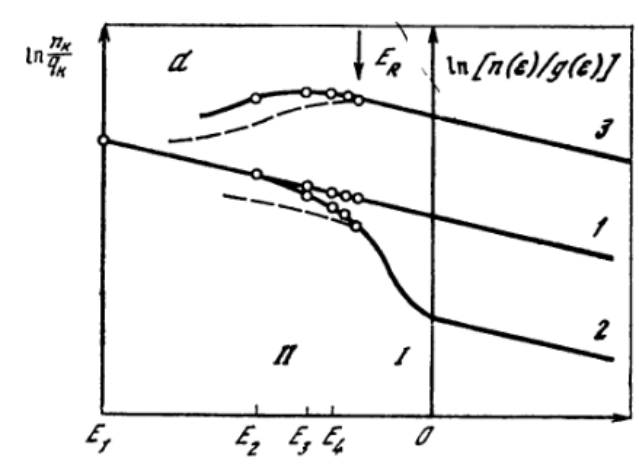
\includegraphics[width=0.5\linewidth]{excited_molecules.png}
	\end{center}
	\caption{Схема, поясняющая характерные распределения атомов по возбужденным состояниям~\cite{biberman}}
	\label{fig:excited_molecules}
\end{figure}

Излучение плазмы обедняет заселенность возбужденных состояний, замедляет ионизацию, ускоряет рекомбинацию. Характерно, что роль радиационных процессов резко уменьшается по мере приближения к границе непрерывного спектра~\cite{biberman}.

Населенности уровней определяются системой кинетических плазмохимических уравнений баланса, записанной для каждого из возбужденных состояний с учетом всевозможных элементарных процессов, обедняющих или населяющих данный уровень.

Важнейшние процессы -- (1) возбуждение/тушение электронным ударом; (2) ионизация электронным ударом	и тройная рекомбинация; (3) возбуждение и тушение при столкновении с атомом в основном состоянии; (4) ионизация в атом-атомных столкновениях и трехчастичная рекомбинация; (5) ассоциативная ионизация и диссоциативная рекомбинация; (6) спонтанные радиационные переходы между дискретными состояниями; (7) радиационная рекомбинация и фотоионизация~\cite{biberman}:

\begin{align*}
	(1)\;A_k + e &\leftrightarrow A_m + e;\\
	(2)\;A_k + e &\leftrightarrow A^{+} + 2e;\\
	(3)\;A_k + A_1 &\leftrightarrow A_m + A_1;\\
	(4)\;A_k + A_1 &\leftrightarrow A^{+} + e + A_1;\\
	(5)\;A_k + B &\leftrightarrow AB^{+} + e;\\
	(6)\;A_k &\rightarrow A_m + \hbar\omega;\;k>m\\
	(7)\;A_k + \hbar\omega &\rightarrow A^{+} + e;\;\hbar\omega\geq E_k\\
\end{align*}

Уравнение, определяющее концентрацию возбужденных частиц в $k$-м состоянии:

\begin{equation*}
	\dv{n_k}{t} = \sum\limits_{m, q}(n_m\omega_{mk}^q-n_k\omega_{km}^q)+F_k-n_kG_k,
\end{equation*}

где $\omega_{km}^q$ -- вероятность перехода из $k$ в $m$ в процессе $q$. Суммирование проводится по всем дискретным состояниям. $F_k$ -- источник образования атомов в $k$-м состоянии за счет процессов, в которых не участвует рассматриваемый атом или его ион (например, диссоциативная рекомбинация с образованием возбужденного атома в $k$-м состоянии). Группа процессов $G_k$ описывает гибель возбужденных атомов в результате процессов, в которых не образуются атомы рассматриваемого элемента ни в основном, ни в возбужденных состояниях (ассоциативная ионизация). Уравнение для концентрации электронов записывается аналогично.

Важно: система уравнений записана в простом случае: не учтены потери частиц на стенках системы, где удерживается плазма (либо потери на периферии), не учтён вылет плазмы и прочие условия.

\section{Динамика заряженных частиц в электрическом и магнитном полях}

Если на не слишком плотную плазму действуют достаточно сильные внешние поля, то в разумном приближении можно пренебречь внутренними полями, происходящими от взаимодействия частиц. В этом приближении можно рассматривать плазму как систему независимых заряженных частиц, движущихся по своим траекториям в заданных внешних полях. Единственным внутренним полем, которым никогда нельзя пренебрегать, является электрическое поле поляризации, возникающее вследствие разделения зарядов и обеспечивающее квазинейтральность плазмы~\cite{frank}.

Рассматривается уравнение движения одной частицы в заданных электромагнитных полях ($e$ -- её заряд; обычно рассматривается электрон, но можно трактовать это обозначение и как заряд рассматриваемой частицы в принципе):

\begin{equation} \label{eq:motion_eq}
	m\dv{\vec{v}}{t} = \frac{e}{c}\left[\vec{v}\times\vec{B}\right]+e\vec{E}
\end{equation}

Аналитически в общем случае не решается.

\subsection{Движение в скрещенных электрическом и магнитном полях}

Скрещённые поля -- поля, перпендикулярные друг другу во всех точках пространства.

Если $\vb{E}=0$, то частица совершает циклотронное вращение ($\vb{B}=B\vb{z_0}$):

\begin{align*}
	m\dv{\vb{v}}{t} &= \frac{e}{c}\left[\vb{v}\times\vb{B}\right];\\
	m\dot{\vb{v}}_x = \frac{e}{c}Bv_y,\;m\dot{\vb{v}}_y &= -\frac{e}{c}Bv_x,\;  m\dot{\vb{v}}_z = 0;\;\\
	\ddot{\vb{v}}_x = -\left(\frac{eB}{mc}\right)^2v_x,\;&\ddot{\vb{v}}_y = -\left(\frac{eB}{mc}\right)^2v_y
\end{align*}

с \uline{циклотронной частотой} $\omega_{Be}=\frac{eB}{mc}$. Циклотронный радиус соответственно: $r_{Be} = \frac{mv_\perp c}{eB}=\frac{v_\perp}{\omega_{Be}}$.

Решение есть движение по круговой орбите вокруг ведущего центра + движение самого ведущего центра вдоль $\vb{B}$, на которое не влияет величина магнитого поля -- т.е. в общем случае траектория движения есть спираль. Направление вращения частицы всегда таково, что создаваемое при этом магнитное поле направлено противоположно внешнему магнитному полю. Следовательно, частицы плазмы стремятся уменьшить магнитное поле, и плазма является диамагнетиком.

Если $E\neq0$, то пусть оно будет направлено по $x$-координате, ведь по условию поля скрещены.

Решением будет (см. раздел~\ref{subsubsec:e_drift}) раскручивающаяся спираль, а если у электрического поля есть ещё компонента вдоль магнитного поля -- то спираль с изменяющимся шагом~\cite{chen}.

Здесь мы не учитывали начальную скорость частицы: так, например, можно показать, что в электрическом поле частица с произвольными н.у. движется по параболе, а в магнитном у нее будет винтовая траектория~\cite{landau2}. 	

\subsection{Дрейфовое приближение, разновидности дрейфового движения}

Есть метод решения -- \uline{дрейфовое приближение} для случая сильного внешнего магнитного поля при пренебрежении взаимодействием между частицами.

При этих условиях движение частицы можно разложить на три составляющие: 
\begin{itemize}
	\item быстрое циклотронное вращение вокруг силовых линий магнитного поля;
	\item дрейфовое движение центра циклотронной окружности поперек магнитного поля (дрейф поперёк поля);
	\item свободное движение вдоль силовой линии, на которое магнитное поле не действует.
\end{itemize}

Различают пять разновидностей дрейфа:
\begin{enumerate}
	\item электрический дрейф: $\vec{E}=const\neq0$;
	\item градиентный дрейф: $\abs{B}\neq const$; 
	\item центробежный дрейф: искривлённые силовые линии магнитного поля;
	\item поляризационный дрейф: $\vec{E}\neq const$;
	\item дрейф под действием сил неэлектромагнитной природы, например, гравитационный дрейф.
\end{enumerate}

Свойства:
\begin{itemize}
	\item скорость направлена не вдоль действующей силы, а перпендикулярно ей и направлению магнитного поля;
	\item постоянная внешняя сила вызывает не равноускоренное, а равномерное движение;
	\item электрическое поле вызывает движение ионов и электронов в одном направлении, а неэлектрические силы возбуждают токи;
	\item если электромагнитное поле слабо неоднородно и медленно меняется во времени, то дрейф носит аддитивный характер и можно рассматривать различные виды дрейфового движения по отдельности.
\end{itemize}

\uline{Условие применимости} теории дрейфа/физичности рассуждений: циклотронное вращение не должно существенно нарушаться. Математически это приводит к двум условиям~\cite{frank}. Во-первых, \uline{условие адиабатичности} -- внешние поля должны мало меняться на длине, равной циклотронному радиусу, и за время, равное периоду циклотронного вращения:

\begin{equation*}
	l_F \gg r_B;\; \tau_F \gg \frac{2\pi}{\omega_B},
\end{equation*}

где $l_F$ и $\tau_F$ -- характерный масштаб и характерное время изменения полей соответственно. Во-вторых, \uline{условие замагниченности} [частицы делятся на замагниченные и не-] -- взаимодействие между частицами не должно заметным образом возмущать циклотронное вращение:

\begin{equation*}
	\omega_B \gg \nu,
\end{equation*}

где $\nu$ -- частота столкновений. Другой вид: время между столкновениями много больше периода обращения по циклотронной окружности. Поскольку $\omega_B = \frac{eB}{mc}$, то для ионов она существенно меньше, чем для электронов, поэтому сначала (при $B\uparrow$) именно электроны становятся замагниченными.

Таким образом, дрейфовое движение есть адиабатическое движение частиц в замагниченной плазме.

Важно: идеальная проводимость -- т.е. $\nu \backsimeq 0$ -- автоматическое выполнение дрейфового приближения.

\subsubsection{Дрейф ``на пальцах''}

[Возможно, такое объяснение будет достаточным, если спрашивают не целиком билет, а в принципе, что такое дрейф, откуда взялся в плазме вообще и т.д.]

Пусть есть магнитное поле, действующее на нас, и мы рассматриваем вращение частицы по ларморовской окружности (по часовой стрелке). Пусть сила $F_\perp$ действует поперек магнитному полю в плоскости рисунка слева направо (рис.~\ref{fig:drift_explanation}). В верхней и нижней половинах окружности сила действует по и против направления вращения соответственно. В результате частица будет двигаться сверху вниз быстрее, чем снизу
вверх. Разность этих скоростей приведет к смещению
циклотронного кружка с постоянной скоростью в направлении, перпендикулярном как к магнитному полю, так и к действующей силе -- дрейф~\cite{frank}. 

\begin{figure}[ht]
	\begin{center}
		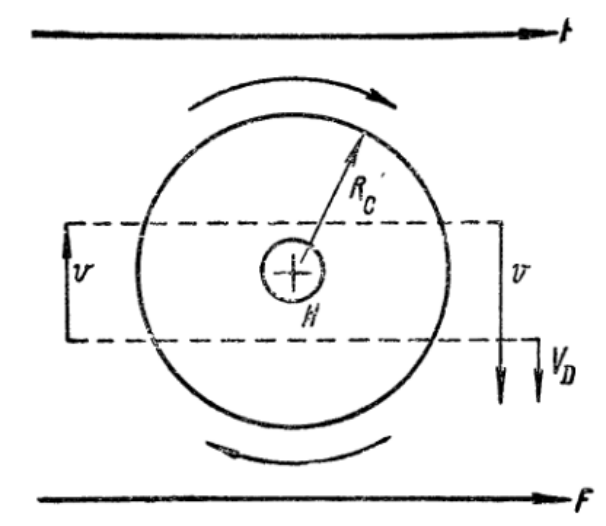
\includegraphics[width=0.5\linewidth]{drift.png}
	\end{center}	
	\caption{Схема возникновения дрейфового движения~\cite{frank}}
	\label{fig:drift_explanation}
\end{figure}

Оценим величину скорости дрейфа. Распишем уравнение~\eqref{eq:motion_eq}, подставив туда скорость в виде суммы циклотронного и дрейфового движений, усредняя по периоду циклотронного вращения вдоль траектории частицы~\cite{kotelnikov} и рассматривая пока с заменой $e\vec{E}\rightarrow\vec{F}$:

\begin{align*}
	\vec{v} &= \overrightarrow{v_c} + \overrightarrow{v_d};\\
	m\dv{\overrightarrow{v_c}}{t} &= \frac{e}{c}\left[\vec{v_c}\times\vec{B}\right];\\
	0=m\dv{\overrightarrow{v_d}}{t} &= \frac{e}{c}\left[\vec{v_d}\times\vec{B}\right]+\vec{F};
\end{align*} 

тогда

\begin{equation*}
	\left[\vec{v_d}\times\vec{B}\right]=-\frac{c}{e}\vec{F}\Rightarrow\left[ \left[\vec{v_d}\times\vec{B}\right]\times\vec{B}\right] =-\frac{c}{e}\left[\vec{F}\times\vec{B}\right]\Rightarrow-\overrightarrow{v_d}B^2+\vec{B}\left(\overrightarrow{v_d}\vec{B}\right)=-\frac{c}{e}\left[\vec{F}\times\vec{B}\right]
\end{equation*}

Ввиду того, что $\overrightarrow{v_d}\perp\vec{B}$, имеем:

\begin{equation} \label{eq:drift_common_eq}
	\overrightarrow{v_d} = \frac{c}{e}\frac{\left[\vec{F}\times\vec{B}\right]}{B^2}
\end{equation}

\subsubsection{Электрический дрейф} \label{subsubsec:e_drift}

Здесь в качестве внешней силы $\vec{F}$ выступает сила электрического поля $e\vec{E}$, работает уравнение~\eqref{eq:motion_eq}.

\uline{Нерелятивистский случай}, уравнения движения:

\begin{equation}
    \begin{cases}
        \dv{\vec{r}}{t} = \vec{\upsilon}; \\
        \dv{\vec{p}}{t} = e\vec{E} + \frac{e}{c}[\vec{\upsilon} \times \vec{B}].
    \end{cases}
\end{equation}

Легко видеть, что если перейти в сопутствующую систему, которая движется со скоростью $\overrightarrow{\upsilon_E} = c\frac{\vec{E}\times \vec{B}}{B^2}$, то уравнения движения примут вид~\cite{kotelnikov}:

\begin{equation}
    \begin{cases}
    \dot{v_x}'=  \frac{eB}{mc} v'_y; \\
    \dot{v_y}'= -\frac{eB}{mc} v'_x; \\
    \dot{v_z}'=  \frac{e}{m} E_{\parallel},
    \end{cases}
\end{equation}

где $E_{\parallel}=\left(\vb{E}\cdot\vb{B}\right)\vb{B}/B^2$. Первые два уравнения дают движение по циклотронной окружности, а третье есть движение вдоль магнитного поля. В итоге в сопутствующей системе отсчета имеем спираль. По сути это дрейф нулевого порядка, тут поля постоянные и никаких неоднородностей нет. В плазме, как правило, эта скорость мала по сравнению с тепловой, поэтому этот дрейф относят к первому порядку.

Формально скорость электрического дрейфа превышает скорость света, если $E>B$. Смысл: при околосветовых скоростях надо честно решать \uline{релятивистские} уравнения движения. При этом исходная формула верна и в таком случае, но когда $E/B \ll 1$~\Sidorov [на практике практически невозможно]. Для релятивизма есть более общая формула для $\upsilon_E$, получаемая из преобразований Лоренца:

\begin{equation}
	\overrightarrow{\upsilon_E} = c \frac{1-\sqrt{1-4\xi^2}}{2\xi^2} \frac{\left[\vec{E} \times \vec{B}\right] }{B^2 + E^2},
\end{equation}

где $\xi = \abs{\left[\vec{E} \times \vec{B}\right]/(B^2 + E^2)}\leq1/2$. Легко видеть, что, как в случае $E<B$, так и в обратном, это выражение дает 
скорость меньше скорости света.

Если записать выражение для радиус-вектора ведущего центра (воображаемого центра дрейфующей системы): $\vb{R}=\vb{r} + \frac{\vb{v}' \times \vb{B}}{\omega_H}$, то в сопутствующей с.о. частиц будет заметать цилиндр (т.к. радиус ларморовской окружности постоянный), а в случае лабораторной с.о. будет гофрированная поверхность.

Важно: если замагничены только электроны, то дрейфуют только они и происходит разделение зарядов~\cite{frank}.

\subsubsection{Градиентный дрейф}
\label{subsubsec:gr_drift}

Пусть электрического поля нет, а магнитное неоднородно: направление всюду одинаково, а меняется лишь амплитуда из-за градиента $\nabla B$, перпендикулярного самому полю. Из-за уменьшения поля $B$
в нижней части орбиты частица проходит её по окружности большего
радиуса, чем верхнюю часть траектории. В итоге на каждом ларморовском обороте возникает некомпенсированное смещение поперёк направлению как $B$, так и $\nabla B$.

Вывод из\Sidorov: сила, действующая на электрический диполь -- $\vec{F_e} = (\vec{p}\cdot\nabla)\vec{E}$ ($\vec{p}$ --эл. дипольный момент), для магнитного по аналогии (при условии $rot\vec{B}=0$ -- выполняется в установках, как правило): ``фиктивная'' сила~\cite{frank} $\vec{F_m} = (\vec{\mu}\cdot\nabla)\vec{B}$, где магнитный момент частицы равен $\vec{\mu}=-\frac{mv_\perp^2}{2B}\vec{h} = -\frac{mv_\perp^2}{2B}\frac{\vec{B}}{B}$.

Тогда из~\eqref{eq:drift_common_eq} следует, что

\begin{equation*}
	\overrightarrow{v_d} = -\frac{c}{e}\frac{mv_\perp^2}{2B}\frac{\left[\nabla \vec{B}\times\vec{B}\right]}{B^2}=\frac{v_\perp^2}{2\omega_{B}}\frac{\left[\vec{B}\times\nabla\vec{B}\right]}{B^2}=-\frac{v_\perp^2}{2\omega_{B}}\left[\frac{\nabla\vec{B}}{B}\times\vec{h}\right]
\end{equation*}

Свойства: электроны и ионы в неоднородном магнитном поле
дрейфуют в противоположных направлениях. Однако выражение не зависит от массы частицы при заданной энергии, поэтому скорости дрейфа электрона и иона равны по абсолютной величине,
если равны их энергии~\cite{kotelnikov}.

Выражение для тока, соответствующего градиентному дрейфу, можно выразить через поперечное давление плазмы $P_\perp = n\frac{mv_\perp^2}{2}$~\cite{frank}, где двойка в знаменателе возникает из-за двух степеней свободы, приходящихся на поперечное движение:

\begin{equation*}
	\overrightarrow{j_d} = en\overrightarrow{v_d} = cP_\perp\frac{\left[\vec{B}\times\nabla\vec{B}\right]}{B^3}
\end{equation*}

\subsubsection{Центробежный дрейф}

Изменение направления магнитного поля -- это искривление магнитных силовых линий.
Если центр циклотронного кружка движется по искривленной
силовой линии, то на него действует
центробежная сила, величина которой
$\vec{F_c} = \frac{mv_\parallel^2}{R^2}\vec{R}$, где $R$ -- радиус кривизны силовой линии. Подставим в~\eqref{eq:drift_common_eq}~\cite{frank}:

\begin{equation*}
	\overrightarrow{v_{cf}} = \frac{mv_\parallel^2c}{e}\frac{\left[\vec{R}\times\vec{B}\right]}{R^2B^2}=\frac{v_\parallel^2}{\omega_B}\frac{\left[\vec{R}\times\vec{h}\right]}{R^2},
\end{equation*}

где $\vec{h} = \vec{B}/B$.

Свойства: электроны и ионы в неоднородном магнитном поле дрейфуют в противоположных направлениях. Однако выражение не зависит от массы частицы при заданной энергии, поэтому скорости дрейфа электрона и иона равны по абсолютной величине, если равны их энергии~\cite{kotelnikov}.

Выражение для тока, соответствующего центробежному дрейфу, можно выразить через продольное давление плазмы $P_\parallel = nmv_\parallel^2$~\cite{frank}:

\begin{equation*}
	\overrightarrow{j_{cf}} = en\overrightarrow{v_{cf}} = cP_\parallel\frac{\left[\vec{R}\times\vec{B}\right]}{R^2B^2}
\end{equation*}

\subsubsection{Поляризационный дрейф}

Если частицы испытывают постоянное или медленно
меняющееся ускорение $\vb{\dot{v}}$, то это можно учесть вводом в рассмотрение инерционной силы~\cite{frank} $\vb{F^{*}}=-m\cdot v$. Инерционные силы вызывают инерционный дрейф, проявляющийся в соответственном дрейфовом токе. Важнейшим случаем инерционного дрейфа является поляризационный дрейф, где ускорение происходит от изменения
скорости электрического дрейфа, вызванного переменным
электрическим полем. Рассмотрим его скорость: $\overrightarrow{v_E} = c\frac{\vec{E}\times\vec{B}}{B^2}$. При учёте изменения электрического поля во времени получаем (с учётом~\eqref{eq:drift_common_eq}):

\begin{equation*}
	\overrightarrow{v_p} = \frac{c}{e}\frac{{-mc\frac{\dot{\vec{E}}\times\vec{B}}{B^2}}\times\vec{B}}{B^2}=\frac{mc^2}{eB^4}\left[\vec{B}\left[\dot{\vec{E}}\vec{B} \right]\right] = \frac{mc^2}{eB^2}\dot{\vec{E}}-\frac{mc^2}{eB^4}\vec{B}\left(\dot{\vec{E}}\cdot\vec{B}\right) 
\end{equation*}

Рассмотрим простейший случай: электрическое и магнитное поля перпендикулярны. Тогда

\begin{equation*}
	\overrightarrow{v_p} = \frac{mc^2}{eB^2}\dot{\overrightarrow{E_\perp}} = \frac{c}{\omega_BB}\dot{\overrightarrow{E_\perp}} \Rightarrow\overrightarrow{j_p}=\frac{nmc^2}{B^2}\dot{\overrightarrow{E_\perp}}=\frac{\rho c^2}{B^2}\dot{\overrightarrow{E_\perp}},
\end{equation*}

где $\rho$ -- плотность плазмы. Плотность дрейфового тока пропорциональна массе
частицы, так что он переносится практически целиком ионами. Кроме того, она зависит от заряда, поэтому в переменном поле плазма поляризуется. Поскольку плазма это проводник, постоянную поляризацию разделенными зарядами создать нельзя, но когда есть переменное электрическое поле, возникает переменный 
поляризационный ток и он вызывает реальную поляризацию плазмы~\cite{kotelnikov}.

Этот дрейфовый ток во многих случаях оказывается гораздо существеннее, чем ток, происходящий от поперечной проводимости плазмы. Он аналогичен току смещения, возникающему при поляризации диэлектриков~\cite{frank}, если ввести диэлектрическую проницаемость $\varepsilon_\perp=1+\frac{4\pi\rho c^2}{B^2}$.

Если $\varepsilon_\perp \gg 1$, то фазовая скорость распространяющейся волны будет равна $u_A = \frac{c}{n_\perp} \approx \frac{B}{\sqrt{4\pi\rho}}$ -- \uline{альфеновская скорость}~\cite{frank}.

Условие применимости [ещё раз]: частоты всех процессов малы по сравнению с наименьшей из циклотронных, т.е. с $\omega_{Bi}$~\cite{frank}.

\subsubsection{Дрейф под действием сил неэлектромагнитной природы: гравитационный дрейф}

Пусть в качестве малой силы в уравнении~\eqref{eq:drift_common_eq} выступает гравитационная сила $\vec{F}=m\vec{g}$. Скорость такого дрейфа $\overrightarrow{\upsilon_g}=\frac{mc}{e}\frac{\left[\vec{g}\times\vec{B}\right]}{B^2}$ зависит от заряда и массы частицы, вызывая ток. Величина обычно пренебрежимо мала~\cite{kotelnikov}, однако из-за неё может возникнуть центробежный дрейф и привести к т.н. гравитационной неустойчивости плазмы.

\subsubsection{Дрейф в неоднородном электрическом поле}

Разложим электрическое поле в сопутствующей с.о., движущуюся воедино с ведущим центром (здесь $\vec{\rho}$ -- радиус-вектор частицы в поперечном сечении)~\cite{kotelnikov}: $\vec{E} = \overrightarrow{E_0}+0+\frac{1}{4}\rho^2\nabla_\perp^2E_0$ и опустим индекс у поля, получаем для добавки к электрическому дрейфу:

\begin{equation*}
	\overrightarrow{\upsilon_{\nabla E}} = \frac{c\rho}{4B^2}\left[\nabla_\perp^2E\times\vec{B}\right]
\end{equation*}

Сколь бы ни мала была поправка, благодаря ей скорость дрейфа различна для
электронов и ионов. Как следствие, электрический дрейф в неоднородном электрическом поле создаёт электрический ток, который
приводит к разделению зарядов. Это явление известно как \uline{эффект
конечного ларморовского радиуса}, существенным
образом влияющий на устойчивость плазмы.

\subsection{Заряженная частица в высокочастотном поле}

Это понятие тесно связано с понятием \uline{высокочастотного (ВЧ) давления}~\cite{chen}. Рассмотрим нерелятивистский случай.

\begin{equation*}
	m\dv{\vb{v}}{t}=-e\left[\vb{E}(\vb{r})+\frac{1}{c}\vb{v}\times\vb{B}(\vb{r})\right],
\end{equation*}

где имеется ВЧ электромагнитное поле (волна): $\vb{E}=\Re\vb{E}(\vb{r})e^{-i\omega t}, \vb{B}=\Re\vb{B}(\vb{r})e^{-i\omega t}$, где $\vb{E}(\vb{r}), \vb{B}(\vb{r})$ -- медленно меняющиеся в пространстве амплитуды (по сравнению с характерным ларморовским радиусом). Тогда движение разбивается на медленный дрейф и быстрые осцилляции: $\vb{r}=\vb{R}+\vb{\rho}$. 

Первый порядок: магнитное поле убираем (нерелятивизм), берём первый порядок электрического поля $\vb{E}(\vb{r})=\vb{E}(\vb{R}) + (\vb{\rho}\nabla)\vb{E}(\vb{R})$ -- уравнение движения имеет следующий вид:

\begin{equation}
    \label{eq:RF_field_particle}
    \vb{\rho} = \frac{e}{m\omega^2} \vb{E}(\vb{R}) \cos(\omega t)
\end{equation}

Второй порядок: учтём, что из уравнений Максвелла $\vb{B} = -\frac{1}{\omega}\nabla\times\vb{E}(\vb{R})\sin(\omega t)$, тогда 

\begin{equation*}
	\dot{\vb{v}} = -\frac{e}{m} \left[(\vb{\rho}\nabla)\vb{E}(\vb{R}) + \vb{v}\times\vb{B}\right] = -\frac{e}{m}\left[ (\vb{\rho}\nabla)\vb{E}(\vb{R})-\frac{1}{\omega}\dot{\vb{\rho}}\times\left[ \nabla\times\vb{E}(\vb{R})\right] \sin(\omega t)\right]
\end{equation*}

Усреднив по периоду $2\pi/\omega$ и подставляя из~\eqref{eq:RF_field_particle}, получим выражение для \uline{пондеромоторной силы}:

\begin{equation*}
	\ddot{\vb{R}} = -\frac{e^2}{2m\omega^2}\left(\vb{E}\nabla)\vb{E} +\vb{E}\times\left[\nabla\times\vb{E}\right]\right)
\end{equation*}

\begin{equation}
    \vb{f}_{RF\_P}=m\ddot{\vb{R}}=-\frac{e^2}{4 m \omega^2} \nabla \abs{E}^2.
\end{equation}

Сила, действующая на единицу объёма плазмы,
получается, если умножить силу на	 плотность электронов. Пользуясь тем, что $E_0 = 2\left\langle E^2 \right\rangle $,
получаем следующую формулу для силы ВЧ-давления:

\begin{equation*}
	\vb{F}_{RF\_P} = -\frac{\omega_{pe}^2}{\omega^2}\nabla\frac{\left\langle E^2 \right\rangle}{2}
\end{equation*}

Суть: электроны осциллируют вдоль направления электрического поля, но магнитное искажает их траектории так, что средняя за период вращения скорость частиц не равна нулю и она смещаются в направлении $\sim\vb{E}\times\vb{B}$. В неоднородной волне электроны будут накапливаться там, где напряженность электрического поля меньше,
и для преодоления возникающего при этом пространственного заряда потребуется дополнительная сила. Именно поэтому эффективное значение силы пропорционально градиенту квадрата поля~\cite{chen}.

Хотя сила действует главным образом на электроны, эта сила при посредстве низкочастотных движений или постоянных полей может влиять и на ионы. Если электроны под действием силы будут сгруппированы в сгустки, то в плазме произойдет разделение зарядов и возникнет электрическое поле. Полная сила, действующая на электроны, будет равна

\begin{equation*}
	\vb{F_e} = -e\vb{E}_\text{разд}+\vb{F}_{RF\_P}
\end{equation*}

Сила ВЧ-давления, действующая на ионы, в $M/m$ раз меньше силы, действующей на электроны, и ею можно пренебречь. Следовательно, на ионы будет действовать только $\vb{F_i} = e\vb{E}_\text{разд}$ Складывая два последних равенства, приходим к выводу, что полная сила, действующая на плазму, равна $\vb{F}_{RF\_P}$.

С действием силы ВЧ-давления непосредственно связана самофокусировка лазерного излучения в плазме. На плазму, через которую проходит лазерный пучок конечного диаметра, действует сила ВЧ-давления, направленная от оси пучка наружу. Эта сила выталкивает плазму из пучка, вследствие чего плазменная частота и диэлектрическая проницаемость внутри пучка становятся меньше, чем снаружи. Плазма при этом действует как собирающая линза, фокусирующая лазерное излучение в пучок меньшего диаметра~\cite{chen}.

\subsection{Понятие адиабатического инварианта}

Из классической механики хорошо известно, что если в системе есть периодическое движение, то действие $S=\oint\vb{p}\dd q$, где интеграл берется по периоду, является интегралом движения. Здесь $p$ и $q$ -- периодические обобщенный импульс и обобщенная координата. Если в системе происходят медленные изменения (т.е. медленно меняющиеся по сравнению с периодом движения) и движение не является чисто периодическим, то интеграл движения остается неизменным и поэтому его называют адиабатическим инвариантом. Существует три адиабатических инварианта, которые соответствуют различным типам периодических движений~\cite{chen}.

\subsubsection{Первый адиабатический инвариант}

В пренебрежении столкновениями площадь потока магнитного поля $\Upphi=\pi\rho B$ через ларморовскую окружность в сопутствующей с.о. является адиабатическим инвариантом, что следует из закона Фарадея: $\mathcal{E}=-\dot{\Upphi}/c$, где по законе Ома $\mathcal{E}=IR=0$, т.к. сопротивления нет.

Для случая частицы, движущейся в однородных электрическом и магнитных полях, в общем случае адиабатический инвариант есть (отличие от формулы выше в $2\pi$ раз -- формальность):

\begin{equation*}
    J_\perp = \frac{1}{2\pi} \oint \vb{P}_{\perp} \dd\vb{r}_{\perp},
\end{equation*}

где интеграл берется по периоду вращения частицы в сопутствующей с.о. Далее можно получить~\cite{kotelnikov}, что:

\begin{equation*}
	J_\perp = \frac{1}{2\pi} \oint \left(m\vb{v}_\perp+\frac{e}{c}\vb{A}_\perp\right)  \dd\vb{r}_{\perp} = \frac{1}{2\pi} \oint m\left(\vb{v}_\perp \cdot \dd\vb{r}_{\perp}\right) +\frac{e}{2\pi c}\int\left(rot(\vb{A})\cdot\dd\vb{S} \right),
\end{equation*}

где $\dd\vb{S}$ -- элемент поверхности, охватываемой контуром интегрирования. Тогда

\begin{equation*}
	J_\perp = \frac{mv_\perp^2}{\omega} - \frac{e}{2\pi c}\vb{B}\int \dd S = \frac{mv_\perp^2}{\omega_c} - \frac{e}{2\pi c}B\pi\frac{v_\perp^2}{\omega_c^2} = \frac{mv_\perp^2}{\omega_c}-\frac{mv_\perp^2}{2\omega_c}=\frac{mv_\perp^2}{2\omega_c}
\end{equation*}

Часто вместо него используют (и называют первым адиабатическим вариантом) магнитный момент частицы $\mu = \frac{mv_\perp^2}{2B}$.

Другой способ доказательства из~\cite{chen}. Рассмотрим теперь магнитное поле, направленное в основном вдоль
оси $z$. Пусть поле осесимметричное, $B_\theta = 0$, $\pdv{}{\theta} = 0$, а напряженность его зависит от $z$. Из уравнения Максвелла $rot(\vb{B})=0$ следует:

\begin{equation*}
	B_r = -\frac{1}{2}r\pdv{B_z}{z}\bigg|_{r=0}
\end{equation*}

Тогда компоненты силы Лоренца вдоль направления магнитного поля равна $F_z=-\frac{e}{c}v_\theta B_r = \frac{e}{2c}v_\theta r\pdv{B_z}{z}$. Рассмотрим проекцию уравнения движения на направление $\vb{B}$ для частицы вблизи оси системы ($v_\theta\approx v_\perp$):

\begin{equation*}
	m\dv{v_\parallel}{t} = \frac{e}{2c}\frac{v_\perp^2}{\omega_c} \pdv{B_z}{z}= \frac{1}{2}\frac{mv_\perp^2}{B} \pdv{B_z}{z}=-\mu\pdv{B}{s}
\end{equation*}

Умножим слева и справа на $v_\parallel=\dv{s}{t}$:

\begin{equation*}
	\dv{}{t}\left(\frac{mv_\parallel^2}{2}\right)=-\mu\pdv{B}{s}\dv{s}{t}=-\mu\dv{B}{t}
\end{equation*}

Значит, 

\begin{equation*}
	-\mu\dv{B}{t} = \dv{}{t}\left(\frac{mv_\parallel^2}{2}\right) = -\dv{}{t}\left(\frac{mv_\perp^2}{2}\right)=-\dv{\mu B}{t} = -\mu\dv{B}{t}-B\dv{\mu}{t}\Rightarrow \dv{\mu}{t}=0
\end{equation*}

В общем случае ``настоящими'' адиабатическими инвариантами (магнитный момент $\mu$ даже в релятивизме формально не является адиабатическим инвариантом, т.к. преобразуется при переходе из одной с.о. в другую, поэтому всегда имеется в виду ``$\mu$ в с.о. ведущего центра'') являются следующие величины: $\Upphi$, $\gamma^2 \mu$, $p_{\perp}^2/B$~\cite{kotelnikov}.

Периодическим движением, соответствующим этому инварианту, является ларморовское вращение. Выберем в качестве обобщённого импульса момент количества движения $p=mv_\perp r$, а координаты $q=\theta$, то действие запишется в виде:

\begin{equation*}
	S=\oint\vb{p}\dd q = \oint mv_\perp r_{L} \dd\theta = 2\pi mv_\perp r_{L} = 4\pi\frac{m}{e}\mu,
\end{equation*} 

где $r_L$ -- ларморовский радиус. Здесь неявно предполагалось, что $\frac{\omega}{\omega_c}\ll 1$. На самом деле $\mu$ -- инвариант даже при $\omega<\omega_c$. На практике это значит, что за один период вращения величина $\mu$ оказывается значительно ближе к константе, чем $\vb{B}$~\cite{chen}.

Примеры НЕприменимости:

\begin{itemize}
	\item магнитная накачка (изменение магнитного поля во времени) с учётом столкновений; 
	\item циклотронный нагрев (взаимодействие с электромагнитной волной с частотой $\omega=\omega_c$)
	\item магнитные каспы (в центре такой магнитной ловушки $\vb{B}=0\Rightarrow\omega_c=0$)
\end{itemize}

\subsubsection{Второй адиабатический инвариант}

Рассмотрим частицу, удерживаемую между двумя магнитными зеркалами. Она колеблется между ними, совершая периодическое движение с так называемой баунс-частотой. Интеграл этого движения записывается в виде $\oint mv_\parallel \dd \vb{s}$, где $\dd \vb{s}$ -- элемент длины при движении ведущего центра вдоль силовой линии. Вследствие того что ведущий центр дрейфует поперек силовых линий, движение не является чисто периодическим и интеграл движения оказывается адиабатическим инвариантом. Он называется \uline{продольным инвариантом} $J$ и вычисляется для половины цикла движения между двумя точками поворота~\cite{chen}:

\begin{equation*}
	J = \int\limits_{s_0}^{s_\text{разворот}}v_\parallel\dd\vb{s}
\end{equation*}

Пример НЕприменимости: т.н. времяпролетная магнитная накачка. Предположим, что к катушкам пробкотрона подводятся переменные токи, так что пробки попеременно приближаются и отдаляются друг от друга с частотой, близкой к баунс-частоте. Частицы, которые колеблются с этой баунс-частотой, всегда будут видеть сближающиеся пробки и, следовательно, их скорость $v_\parallel$ будет увеличиваться. В этом случае $J$ не сохраняется, поскольку изменение поля $\vb{B}$ происходит на временных масштабах, которые нельзя считать большими по сравнению с временем колебания частиц между зеркалами.

\subsubsection{Третий адиабатический инвариант}

В магнитной ловушке частица движется от одного конца к другому, смещаясь вдоль экватора, заметая некую поверхность -- дрейфовую оболочку. Если магнитное поле и потенциал медленно меняются, сохраняется магнитный поток через сечение дрейфовой оболочки:

\begin{equation*}
     \Upphi_{dr}= \int\limits_{S_{dr}} \vb{B}\dd\vb{S}.
\end{equation*}

Инвариант $\Upphi_{dr}$ применяется редко, поскольку большинство флуктуации магнитного поля $\vb{B}$ происходит на временных масштабах, которые малы по сравнению с периодом дрейфа, отвечающим этому инварианту~\cite{chen}.

Пример НЕприменимости: возбуждение МГД-волн в ионосфере. Эти волны имеют большой период, сравнимый со временем перемещения частицы вокруг Земли. Следовательно, частицы после одного оборота могут встретить волну в той же самой фазе. Если это происходит, то передача энергии от дрейфующих частиц к волне может привести к ее раскачке.

\section{Магнитная гидродинамика плазмы}

Важное условие влияния магнитного поля на плазменную ``жидкость'': $\omega_B\tau_{tr}\gtrsim 1$, где транспортное $\tau_{tr}$ -- время свободного пробега [если $gg 1$ -- то бесстолкновительный случай]\Tokman.

\subsection{Уравнения движения плазмы в магнитном поле, проникновение магнитного поля в плазму. Двухжидкостная гидродинамика}

Здесь и ниже будем рассматривать только простую плазму -- состоящую из электронов и ионов одного сорта. Запишем уравнения \uline{двухжидкостной} гидродинамики. Их вывод смотри в~\ref{subsubsec:hydrodynamic_description}:

\begin{align*}
	\pdv{n_\alpha}{t}+\div{ \left( n_\alpha \vb{v}_\alpha \right) } &= 0;\\
	m_\alpha n_\alpha \left( \pdv{\vb{v}_\alpha}{t} +(\vb{v}_\alpha \cdot\grad )\vb{v}_\alpha \right) &= -\grad{P_\alpha} + e_\alpha n_\alpha\vb{E} + \frac{e_\alpha n_\alpha}{c}[\vb{v}_\alpha \times \vb{B}] + \vb{F}_{fric,\alpha},
\end{align*}

где $\alpha = e, i$; $\vb{F}_{fric,\alpha}$ -- эффективная сила трения на сорт частиц $\alpha$ со стороны другого сорта. Для решения данной системы уравнения нужно написать условие связи на поля -- т.е. уравнения Максвелла:

\begin{align*}
	\curl\vb{E} &= -\frac{1}{c}\pdv{\vb{B}}{t}; \\
	\curl\vb{B} &= \frac{4\pi}{c}\vb{j}; \\
	\div{\vb{B}} &= 0;\\
	\rho_e &= 0,
\end{align*}

где $\partial\vb{E}/\partial t$ положено равным нулю, т.к. мы будем рассматривать процессы со скоростями сильно медленнее скорости света. Последнее равенство говорит, что мы рассматриваем квазинейтральную (незаряженную) плазму. Величины $\rho_e$ и $\vb{j}$ определяются следующим образом:

\begin{align*}
	\rho_e &= \sum_\alpha e_\alpha n_\alpha = e n_i - e n_e;\\
	\vb{j} &= \sum_\alpha e_\alpha n_\alpha \vb{v}_\alpha = e n_i \vb{v}_i - e n_e \vb{v}_e.
\end{align*}

Сложим соответственные уравнения для электронов и ионов и перейдём к рассмотрению элемента массы плазмы $\rho = m_en_e + m_in_i\approx m_in_i$, движущейся со скоростью массопереноса $\vb{V} = (m_e n_e \vb{v}_e + m_i n_i \vb{v}_i)/\rho\approx (m_in_i\vb{v}_i)/(m_in_i)=\vb{v}_i$ [$m_e \ll m_i$]:

\begin{align*}
	\pdv{\rho}{t} + \div{\left(\rho \vb{V}\right)} &= 0; \\
	\rho\left( \pdv{\vb{V}}{t} + (\vb{V}\cdot\grad)\vb{V} \right) &= -\grad{P} + \frac{1}{c}[\vb{j}\times\vb{B}],
\end{align*}

где $P = P_e+P_i$. По сути эти уравнения -- гидродинамические уравнения, описывающие проводящую жидкость. Так как здесь явно нет ионов и электронов -- это уравнения \textit{одножидкостной} гидродинамики.
Обычно $\vb{j}$ в уравнении Эйлера выражают из уравнений Максвелла: $\vb{j} = c/4\pi\curl\vb{B}$.

Ещё в эти уравнения неявно включение уравнение состояния (например, предположение о несжимаемой жидкости $\div{V}=0$, изотерма $T=const$, адиабата $PV^\gamma=const$ или др.)~\cite{kroll}.

Для окончательного замыкания уравнений гидродинамики и уравнений Максвелла нам нужен закон Ома, т.е. зависимость между векторами $\vb{j}$ и $\vb{E}$. 

\begin{enumerate}
	\item Вывод Токмана\Tokman

Вернёмся к уравнению Эйлера для электронов (см. выше или см.~\eqref{eq:Euler_eq}). Так как с помощью гидродинамики мы описываем процессы на масштабах существенно более медленные, чем, например, столкновения, то запишем уравнение Эйлера в пределе малых частот $\omega \ll \nu_{ei}^t$, где $\omega$ -- характерная частота процесса, $\nu_{ei}^t$ -- частота столкновений. В таком случае слагаемое $m_en_e\dd\vb{v}_e/\dd t$ в левой части много меньше, чем сила трения в правой части, которую за счёт $\vb{j} = e (n_i \vb{v}_i - n_e \vb{v}_e)\approx e n (\vb{v}_i - \vb{v}_e)$ [квазинейтральность] можно записать в виде $\nu m_en_e(\vb{v}_e-\vb{v}_i)=-\nu m_e\vb{j}/e$. Итого имеем:

\begin{equation*}
	0 \approx -\grad{P_e} - e n_e \vb{E} - \frac{e}{c}[\vb{v}_e \times \vb{B}] + \frac{\nu m_e}{e}\vb{j}
\end{equation*}

\begin{equation} \label{eq:Ohm_eq}
	\vb{j} = \frac{e^2n_e}{m_e\nu_{ei}^t}\vb{E}+ \frac{e^2n_e}{m_e\nu_{ei}^tc}[\vb{v}_e \times \vb{B}]+\frac{e}{m_e\nu_{ei}^t}\grad{P_e}
\end{equation}

Подставим сюда $\vb{v}_e = \vb{v}_i - \frac{\vb{j}}{en} = \vb{V} - \frac{\vb{j}}{en}$:

\begin{equation*}	
	\vb{j} = \sigma \left( \vb{E} + \frac{1}{c}[\vb{V}\times\vb{B}] - \frac{1}{cen}[\vb{j}\times\vb{B}] + \frac{1}{en}\grad{P_e} \right)
\end{equation*}

где $\sigma = \frac{e^2 n_e}{m \nu_{ei}^t}$.

Рассмотрим теперь уравнение одножидкостной гидродинамики в том же приближении $\omega \ll \nu$, т.е. по сути будем искать состояние равновесия. Получим:

\begin{equation*}
	0 \approx -\grad{\left( P_e + P_i \right)} + \frac{1}{c}[\vb{j}\times\vb{B}]
\end{equation*}

Подставляя это в уравнение~\eqref{eq:Ohm_eq} получаем окончательный вид закона Ома:

\begin{equation*}
	\vb{j} = \sigma \left( \vb{E} + \frac{1}{c}[\vb{V}\times\vb{B}] - \frac{1}{en}\grad{P_i} \right)
\end{equation*}

Оценим по порядку величины второе и третье слагаемые. Сравним второе с первым:

\begin{align*}
	\curl\vb{E} = -\frac{1}{c}\dv{\vb{B}}{t} \\
	B \sim \frac{c\tau}{L} E = \frac{c}{V} E
\end{align*}

Следовательно, второй член одного порядка с первым. Сравним третье слагаемое со вторым:

\begin{align*}
	\frac{1}{n e}\grad P_i \sim \frac{n T}{n e L} = \frac{T}{eL} \\
	\frac{VB}{c}\;\text{vs}\;\frac{T}{eL} \leftrightarrow V\;\text{vs}\;\frac{cT}{eBL} \sim v_{d},
\end{align*}

где $v_{d}$ --- скорость дрейфа в неоднородном поле (см.~\ref{subsubsec:gr_drift}). Этим слагаемым можно пренебречь, когда рассматривается медленное и крупномасштабное движение, но достаточно быстрое в сравнении с дрейфом. Обычно работаем именно в таком приближении:

\begin{equation*}
	\vb{j} = \sigma \left( \vb{E} + \frac{1}{c}[\vb{V}\times\vb{B}]\right)
\end{equation*}

\item Вывод Котельникова~\cite{kotelnikov}

Просто предположим линейную зависимость между током $\vb{j}$ и электрическим полем в системе отсчёта, движущейся с элементом плазмы $\vb{E}'$. Преобразование Лоренца в лабораторную систему при малых скоростях $V \ll c$ имеет вид:

\begin{equation*}
	\vb{E}' = \vb{E} + \frac{1}{c}[\vb{V}\times \vb{B}],
\end{equation*}

тогда закон Ома имеет вид:

\begin{equation*}
	\vb{j} = \Sigma\left( \vb{E} + \frac{1}{c}[\vb{V}\times \vb{B}] \right)
\end{equation*}

\end{enumerate}

\uline{Итоговая система одножидкостной МГД}:

\begin{align}
	\label{eq:MGD_curlB_eq} \curl{\vb{B}} &= \frac{4\pi}{c}\vb{j};\\
	\label{eq:MGD_Ohm_eq} \vb{j} &= \sigma\left(\vb{E} + \frac{1}{c}[\vb{V}\times\vb{B}] \right); \\
	\curl{\vb{E}} &= -\frac{1}{c}\pdv{\vb{B}}{t}; \\
	\div{\vb{B}} &= 0; \\
	\pdv{n}{t} &+ \div{\left(n\vb{V}\right)} = 0; \\
	\label{eq:MGD_motion_eq} n M \dv{\vb{V}}{t} &= \frac{1}{4\pi}\left[\left[\curl{\vb{B}} \right]\times\vb{B}\right]-\grad{P}. 
\end{align}

[Плюс ещё должно быть уравнение состояния].

Возьмём ротор от уравнения~\eqref{eq:MGD_curlB_eq} и подставим~\eqref{eq:MGD_Ohm_eq}:

\begin{align}
	&\curl{[\curl{\vb{B}}]} = \frac{4\pi\sigma}{c}\curl{\left( \vb{E} + \frac{1}{c}[\vb{V}\times\vb{B}] \right)} \\ \nonumber
	&-\Delta\vb{B} = \frac{4\pi\sigma}{c^2}\left( -\pdv{\vb{B}}{t} + \curl{[\vb{V}\times\vb{B}]} \right) \\ \nonumber
	&\pdv{\vb{B}}{t} = \curl{[\vb{V}\times\vb{B}]} + \frac{c^2}{4\pi\sigma}\Delta\vb{B} \label{eq:MGD_main_eq}
\end{align}

Это основное уравнение МГД, определяющее эволюцию магнитного поля\Tokman. Оценим слагаемые в правой части:

\begin{align*}
	&\curl{[\vb{V}\times\vb{B}]} \sim \frac{VB}{L} \\
	&\frac{c^2}{4\pi\sigma}\Delta\vb{B} \sim \frac{c^2B}{4\pi\sigma L^2}
\end{align*}

Вводят \uline{магнитное число Рейнольдса} $R_m$ -- отношение этих членов:

\begin{equation*}
	R_m = \frac{4\pi\sigma \cdot L}{c^2}\left\langle V\right\rangle 
\end{equation*}

В зависимости  от величины $R_m$ реализуются различные ситуации:

\begin{enumerate}
	
	\item $R_m \ll 1$ (маленькая проводимость/большой размер плазмы/быстрые потоки):
	
	В таком случае не учитываем слагаемое $\vb{V}\times\vb{B}$ и получаем уравнение:
	
	\begin{equation*}
		\pdv{\vb{B}}{t} = \frac{c^2}{4\pi\sigma}\Delta\vb{B} \equiv D_m\Delta\vb{B}
	\end{equation*}

	Это уравнение диффузии, которое описывает скинирование магнитного поля в плазме [магнитное поле диффундирует в хорошо проводящую (т.е. столкновительную) плазму\Tokman].
	Глубина проникновения (толщина скин-слоя) переменного магнитного поля в плазму оценивается как $\delta = \sqrt{2D_m\tau}$, где $\tau$ -- характерное время колебаний магнитного поля $\tau\sim 1/\omega$, т.е.
	
	\begin{equation*}
		\delta = \frac{c}{\sqrt{2\pi\sigma\omega}}
	\end{equation*}

	Отметим, что точно такое же выражение получается при рассмотрении проникновения переменного ВЧ тока в проводник с конечной проводимостью~\cite{kotelnikov}.
		
	\item $R_m \gg 1$ (большая проводимость):
	
	Этот предел соответствует \uline{идеальной магнитной гидродинамике}. Уравнения в таком случае принимают вид:
	\begin{align}
		\label{eq:iMGD_B} &\pdv{\vb{B}}{t} = \curl{[\vb{V}\times\vb{B}]}; \\
		&\pdv{n}{t} + \divergence{\left( n\vb{V} \right)} = 0;\\
		\label{eq:iMGD_motion} &n M \dv{\vb{V}}{t} = \frac{1}{4\pi}\left[\left[\curl{\vb{B}} \right]\times\vb{B}\right]-\grad{P}.
	\end{align}

	Если $\sigma\rightarrow\infty$, то эволюция магнитного поля $\sim$ движению самой среды -- бездиссипативная динамика.
	
\end{enumerate}

\subsection{Вмороженность магнитного поля} \label{subsec:Alfven_th}

[В зарубежной литературе иногда называется теоремой Альфвена.] Рассматривается идеально проводящая среда/идеальная МГД ($R_m \gg 1$). 

\uline{Качественное описание}: Известно, что если проводник при своем движении пересекает силовые линии магнитного поля, то в нем возбуждается электродвижущая сила. В идеальном проводнике сколь угодно малая электродвижущая сила возбуждала бы бесконечный ток, что невозможно. Следовательно, идеальный проводник должен увлекать с собой магнитные силовые линии так, как если бы они были в него ``вморожены''. Иными словами, идеально проводящая плазма движется так, как если бы ее частицы были ``приклеены'' к силовым линиям магнитного поля~\cite{frank}.

\begin{figure}[ht]
    \begin{center}
    	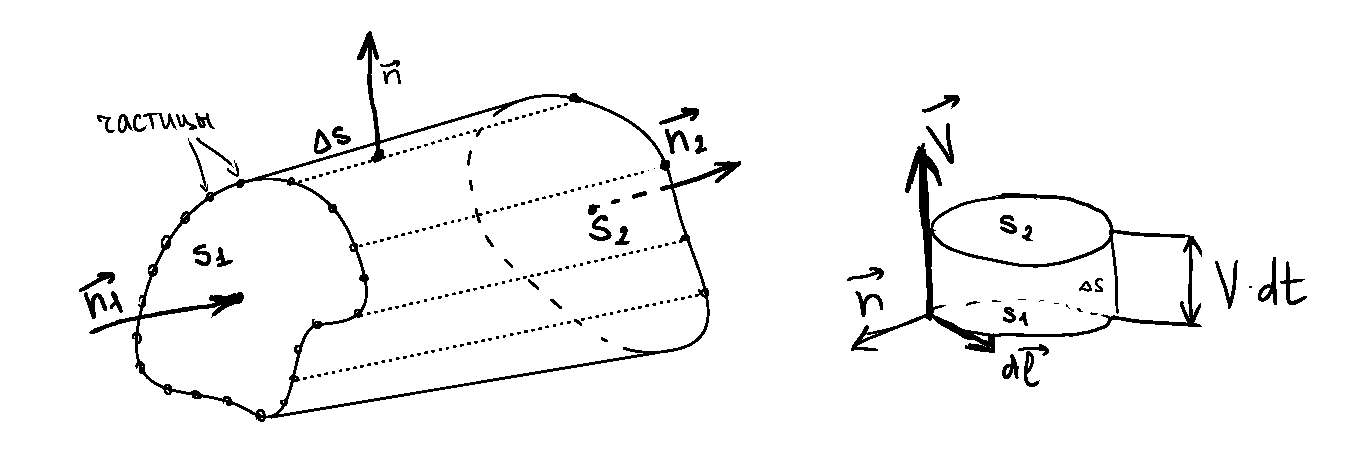
\includegraphics[width=1\linewidth]{5.flow.pdf}
   \end{center}	
    \caption{Геометрия при выводе вмороженности}
    \label{fig:Alfven_th_geom}
\end{figure}

\uline{Доказательство}: Рассчитаем изменение потока магнитного поля за интервал времени $\dd t$ через поверхность ``трубки'', образованной траекториями [лагранжевых] частиц плазмы (см. рис.~\ref{fig:Alfven_th_geom}). Изменение этого потока связано с двумя эффектами: изменением амплитуды магнитного поля и изменением площади поверхности трубки. В приближении бесконечно малых $\dd t$ эти эффекты учитываем независимо, т.е.:

\begin{equation} \label{eq:frozen_in_flow_diff}
	\Phi_2 - \Phi_1 = \iint\limits_S (\vb{B}_2 - \vb{B}_1)\dd \vb{S} + \iint\limits_{S_2 - S_1}\vb{B}_1\dd\vb{S}
\end{equation}

Так как магнитное поле бездивергентно [$div\vb{B}=0$], то его поток через любую замкнутую поверхность равен нулю, т.е.

\begin{equation*}
	\iint\limits_{S_2}\vb{B}_1\dd\vb{S} + \iint\limits_{\Delta S}\vb{B}_1\dd\vb{S} - \iint\limits_{S_1}\vb{B}_1\dd\vb{S} = 0
\end{equation*}

где знак "$-$" перед слагаемым $S_1$ связан с направлением нормали, которую мы выбрали (см. рис.~\ref{fig:Alfven_th_geom}). Из этого равенства следует, что в выражении~\eqref{eq:frozen_in_flow_diff} второй множитель можно вычислить следующим образом:

\begin{equation} \label{eq:frozen_in_flow}	
	\iint\limits_{S_2 - S_1}\vb{B}_1\dd\vb{S} = -\iint\limits_{\Delta S} \vb{B}_1\dd\vb{S} = -\oint\limits_{l_1} \left( \vb{n}\vb{B}_1 \right) \dd l\,V\,\dd t
\end{equation}

где $V\dd t$ -- ``ширина'' ленточной поверхности $\Delta S$, $\vb{n}$ -- нормаль к ней. Эту нормаль можно записать в следующем виде:

\begin{equation*}
	\vb{n} = \frac{[\dd\vb{l}\times\vb{V}]}{\dd l\, V}
\end{equation*}

Тогда выражение~\eqref{eq:frozen_in_flow} записывается в следующем виде:

\begin{equation*}
	\iint\limits_{S_2 - S_1}\vb{B}_1\dd\vb{S} = -\dd t \oint\limits_{l_1} [\dd\vb{l}\times\vb{V}]\vb{B}_1 = -\dd t \oint\limits_{l_1} [\vb{V}\times\vb{B}_1]\dd\vb{l} = -\dd t\iint\limits_{S_1}\curl[\vb{V}\times\vb{B}_1] \dd\vb{S}
\end{equation*}

где в предпоследнем равенстве мы сделали циклическую перестановку в смешанном произведении, а в последнем применили теорему Стокса [$\oint\limits_{l} \vb{F} \dd\vb{l} = \iint\limits_S (\nabla
\times\vb{F})\dd\vb{S}$].

В итоге переписываем уравнение~\eqref{eq:frozen_in_flow_diff}:

\begin{equation*}
	\frac{\Phi_2 - \Phi_1}{\dd t} = \iint\limits_{S_1}\left( \frac{\vb{B}_2 - \vb{B}_1}{\dd t} - \curl[\vb{V}\times\vb{B}_1] \right)\dd\vb{S} \stackrel{\dd t\rightarrow 0}{=} \iint\limits_{S_1}\left( \pdv{\vb{B}}{t} - \curl[\vb{V}\times\vb{B}] \right)\dd\vb{S} = 0
\end{equation*}

где последнее равенство верно в силу уравнений идеальной МГД~\eqref{eq:iMGD_B}. Таким образом, получаем, что поток через любую трубку, образованную траекториями плазмы, является константой. Так как можем взять сколь угодно тонкую трубку, то получается, что силовые линии магнитного поля как бы приклеены к частицам плазмы и совпадают с траекториями частиц.

\uline{Следствия}:

\begin{itemize}
	\item Частицы, находящиеся на одной магнитной линии, всегда будут находиться на одной магнитной линии.
	\item Сохраняется топология магнитного поля, т.е. не допускается появление разрывов в магнитных линиях, например, как в магнитной рекомбинации. Разрешены только топологически непрерывные изменения линий магнитного поля [топологически обратимые преобразования].
	\item Плазма не может расширяться поперёк магнитного поля.
\end{itemize}

Очевидно, что в реальности из-за конечной проводимости все эти эффекты верны только приближённо. Например, магнитное поле может диффундировать в плазму. С другой стороны, это можно трактовать как смещение плазмы поперёк магнитного поля.

Добавление проводимости в уравнения может позволить оценить характерные времена процессов, например, перезамыкания силовых линий магнитного поля (т.е. запрещенных при рассмотрении вмороженности). Два основных способа ``сломать'' наши допущения: учесть конечную $\sigma$, учесть конечное $m_e/m_i$\Tokman.

\subsection{Законы сохранения в идеальной одножидкостной МГД}

В целом уравнения гидродинамики выглядят как уравнения сохранения:

\begin{equation}
	\label{eq:conservation_laws}
	\pdv{n}{t} + \div{\vb{J}} = 0
\end{equation}

где $n$ -- плотность некой величины, а $\vb{J}$ -- её поток.
Явно перепишем уравнения идеальной МГД~\eqref{eq:iMGD_B}--\eqref{eq:iMGD_motion} в форме законов сохранения~\eqref{eq:conservation_laws}. Уравнение непрерывности уже записано в таком виде:

\begin{align}
	\label{eq:conservation_laws_1}
	&\pdv{n}{t} + \divergence{\left( n\vb{V} \right)} = 0 \\
	&\dv{\rho}{t} = 0
\end{align}

По сути это уравнение -- \uline{закон сохранения массы} $\rho = nM$. [Если домножить на заряд -- то будет закон его сохранения.]
Преобразуем уравнение Эйлера~\eqref{eq:iMGD_motion}~\cite{kotelnikov}:

\begin{equation*}
	n M \left( \pdv{\vb{V}}{t} + \left( \vb{V}\cdot\grad \right)\vb{V} \right) = -\grad{P} + \frac{1}{4\pi}\left[\left[ \curl{\vb{B}} \right]\times\vb{B}\right]
\end{equation*}

Распишем последнее слагаемое:
\begin{equation*}
	\left[\left[ \curl{\vb{B}} \right]\times\vb{B}\right] = -\left[\vb{B}\times\left[ \curl{\vb{B}} \right]\right] = -\frac{1}{2}\grad{B^2} + \left( \vb{B} \cdot\grad \right)\vb{B}
\end{equation*}

Это выражение можно записать в тензорном виде:

\begin{equation*}
	\begin{split}
		\left( -\frac{1}{2}\grad{B^2} + \left( \vb{B} \cdot\grad \right)\vb{B} \right)_\nu = -\frac{1}{2}\pdv{B^2}{x_\nu} + B_\mu\pdv{B_\nu}{x_\mu}= -\frac{1}{2}\pdv{}{x_\mu}\left( B^2 \delta_{\mu\nu} \right) + \pdv{}{x_\mu}\left( B_\mu B_\nu \right) - B_\nu\pdv{B_\mu}{x_\mu} =\\= \pdv{}{x_\mu}\left( -\frac{B^2}{2} \delta_{\mu\nu} + B_\mu B_\nu \right)
	\end{split}
\end{equation*}

где было использовано $\partial B_\mu/\partial x_\mu = 0$ ($\div{\vb{B}}=0$). Перенесём все слагаемые влево.

Умножим уравнение~\eqref{eq:conservation_laws_1} на $M\vb{V}$ и сложим с исходным~\eqref{eq:conservation_laws_1} и добавим к уравнению Эйлера. Рассмотрим отдельно слагаемое с дивергенцией:

\begin{equation*}
	V_\nu \pdv{}{x_\mu}\left( nV_\mu \right) + nV_\mu\pdv{V_\nu}{x_\mu} = \pdv{}{x_\mu}\left( nV_\mu V_\nu \right)
\end{equation*}

В итоге уравнение Эйлера переписывается в следующем виде:

\begin{equation*}
	\pdv{}{t}\left( nM\vb{V} \right) + \div{\left( nM\overleftrightarrow{\vb{VV}} + \left( P + \frac{B^2}{8\pi} \right)\overleftrightarrow{\vb{I}} - \frac{1}{4\pi}\overleftrightarrow{\vb{BB}} \right)} = 0
\end{equation*}

\begin{equation*}
	\pdv{}{t}\left( nM\vb{V} \right) + \div{\left( nM\overleftrightarrow{\vb{VV}} + P\overleftrightarrow{\vb{I}} + \overleftrightarrow{\vb{T}} \right)} = 0
\end{equation*}

\begin{equation}
	\label{eq:pulse_dens_change}
	\dv{\vb{\Pi}}{t} = - \div{\left( P\overleftrightarrow{\vb{I}} + \overleftrightarrow{\vb{T}} \right)}
\end{equation}

где $\overleftrightarrow{\vb{I}}$ -- единичный тензор $\delta_{\mu\nu}$, $\overleftrightarrow{\vb{BB}}$ -- обозначение тензора с компонентами $B_\mu B_\nu$.

Таким образом получили аналог \uline{закона сохранения импульса}: $\vb{\Pi}=nM\vb{V}$ -- это плотность импульса, а тензор $\overleftrightarrow{\vb{T}}$ называют \uline{тензором напряжений магнитного поля}. 	

Из уравнения~\eqref{eq:pulse_dens_change} видно, что правая часть этого уравнения имеем смысл плотности силы $\vb{f}$, а полная сила получается интегрированием по объёму $\dd V$, который по теореме Гаусса преобразуется к интегралу по площади, ограничивающей $\dd V$. Таким образом тензоры $P\overleftrightarrow{\vb{I}}$ и $\overleftrightarrow{\vb{T}}$ определяют общую силу, действующую на маленькую площадку $\dd\vb{S}$.
Силу со стороны магнитного поля можно разделить на силу вдоль и поперёк магнитного поля:

\begin{equation*}
	T_{\mu\nu} = \frac{B_\mu B_\nu}{4\pi}-\frac{B^2}{8\pi}\delta_{\mu\nu} = p_m \left( \delta_{\mu\nu} - b_\mu b_\nu \right) - p_m b_\mu b_\nu = p_m (b_\perp - b_\parallel)
\end{equation*}

где $p_m = B^2 / 8 \pi$ -- ``магнитное'' давление. Таким образом, магнитное поле ``тянет'' площадку $\dd \vb{S}$ вдоль своего направления $\vb{B}/B$ и ``давит'' на площадку поперёк своего направления~\cite{kotelnikov}.

Рассмотрим третье уравнение идеальной МГД~\eqref{eq:iMGD_B}:

\begin{equation*}
	\pdv{\vb{B}}{t} = \curl{[\vb{V}\times\vb{B}]}
\end{equation*}

Преобразуем правую часть (ротор от векторного произведения раскрывается с использованием правила стрелок):

\begin{equation*}
	\curl{[\vb{V}\times\vb{B}]} = (\vb{B}\cdot\grad)\vb{V} - (\vb{V}\cdot\grad)\vb{B} - \vb{B}\,\text{div}{\vb{V}} + \vb{V}\,\text{div}{\vb{B}}
\end{equation*}

Распишем по компонентам:

\begin{equation*}
	\curl{[\vb{V}\times\vb{B}]}_\nu = B_\mu \pdv{V_\nu}{x_\mu} - V_\mu \pdv{B_\nu}{x_\mu} - B_\nu\pdv{V_\mu}{x_\mu} + V_\nu\pdv{B_\mu}{x_\mu} = \pdv{}{x_\mu}\left( B_\mu V_\nu - B_\nu V_\mu \right)
\end{equation*}

В итоге вмороженность магнитного поля тоже можно записать в виде некого закона сохранения:

\begin{equation*}
	\pdv{\vb{B}}{t} + \div{\left( \overleftrightarrow{\vb{VB}} - \overleftrightarrow{\vb{BV}} \right)} = 0
\end{equation*}

Вообще говоря, уравнения гидродинамики обычно обрывают на уравнении переноса тепла (см. раздел~\ref{subsubsec:hydrodynamic_description}), которое мы обычно не используем, т.к. оно не важно для рассмотрения волн, неустойчивостей и т.п. Его, очевидно, тоже можно записать в виде \uline{закона сохранения энергии}:

\begin{equation*}
	\pdv{Q}{t} + \div{\vb{q}} = 0
\end{equation*}

где $Q$ -- плотность тепловой энергии $Mn\langle \vb{V}\vb{V} \rangle - Mn\langle V\rangle^2$. Вектор потока тепла $\vb{q}$ в запоминающемся виде не записывается, поэтому я его не пишу.

Если функции распределения локально максвелловские и поля слабые (т.е. нет, например, омического нагрева), то это уравнение переходит в уравнение теплопроводности:

\begin{equation}
	\label{eq:heat_equation}
	\pdv{T}{t} = \div{\left( \chi \grad T \right)}
\end{equation}

где $\chi$ -- коэффициент температуропроводности. Он связан с коэффициентом теплопроводности $\varkappa = \chi/(3/2n)$~\cite{kotelnikov}.

Однако важно понимать, что, вообще говоря, наличие внешнего магнитного поля делает плазму анизотропной, и эта анизотропия проявляется даже в переносе тепла. Кинетическая теория (см.~\ref{subsec:transport_phenomena}) даёт следующее выражение для коэффициента температуропроводности:

\begin{equation*}
	\chi_\alpha \sim  \frac{T_\alpha \tau_\alpha}{m_\alpha}
\end{equation*}

Введём длину свободного пробега $\lambda_\alpha = v_{T_\alpha} / \tau_\alpha$:

\begin{equation*}
	\chi_\alpha \sim \frac{\lambda_\alpha^2}{\tau_\alpha}
\end{equation*}

Выражение в таком виде совместно с уравнением~\eqref{eq:heat_equation} несёт ясный физический смысл: характерный масштаб теплопроводности в пространстве равен $\lambda_\alpha$ и во времени $\tau_\alpha$. При этом наличие магнитного поля не влияет на движение вдоль магнитного поля, значит, эти масштабы должны оставаться такими же.

В движении поперёк магнитного поля появляется ещё один характерный масштаб -- ларморовский радиус. Поэтому в сильном магнитном поле, т.е. если $r_{B\alpha} \sim v_{T_\alpha} / \omega_{B\alpha} \ll \lambda_\alpha$, можно считать, что коэффициент поперечной теплопроводности записывается в следующем виде:

\begin{equation*}
	\varkappa_{\perp\alpha} \sim \frac{n_\alpha \rho_\alpha^2}{\tau_\alpha}
\end{equation*}

\begin{figure}[ht]
	\begin{center}
		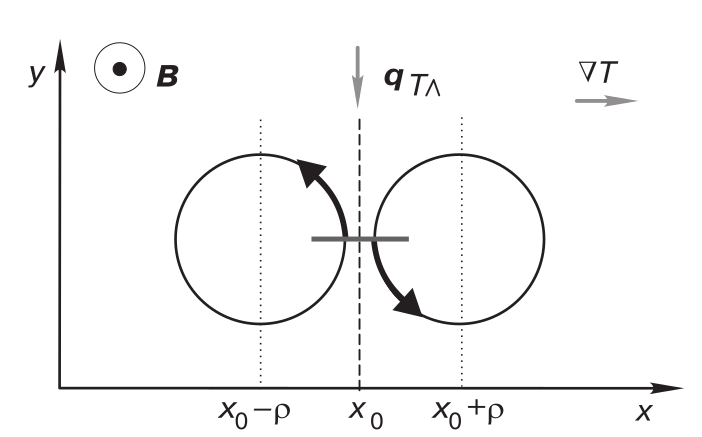
\includegraphics[width=0.5\linewidth]{5.slanted.png}
	\end{center}
    \caption{Возникновение ``косого'' потока тепла~\cite{kotelnikov}}
    \label{fig:oblique_heat_flow} 
\end{figure}

Строго говоря, в замагниченной плазме есть ещё так называемый ``косой'' поток тепла. Его появление связано с тем, что при наличии градиента температур поток энергии через площадку, натянутую на вектора $\vb{B}$ и $\grad T$, оказывается отличен от нуля из-за того, что поток в одну сторону этой площадки создаётся более горячими электронами, а поток в другую -- более холодными (см. рис.~\ref{fig:oblique_heat_flow}).

Легко оценить нескомпенсированный потока тепла в такой ситуации: $q_x \sim n_e v_{T_e} r_{Be} (\partial T_e/\partial x)$. Тогда в уравнении теплопроводности должно быть ещё следующее слагаемое:

\begin{equation*}
	\pdv{Q_e}{t} = \dots + \pdv{}{x}\left( n_e v_{T_e} r_{Be} \pdv{T_e}{x} \right) = \dots + \pdv{}{x}\left(\frac{n_e v_{T_e}^2}{\omega_{Be}}\pdv{T_e}{x} \right)
\end{equation*}

Таким образом, в замагниченной плазме есть три разных коэффициента теплопроводности (продольный, поперечный, косой)~\cite{kotelnikov}:

\begin{align*}
	&\varkappa_{\parallel\alpha} \sim \frac{n_\alpha \lambda_\alpha^2}{\tau_\alpha} \\
	&\varkappa_{\perp\alpha} \sim \frac{n_\alpha \rho_\alpha^2}{\tau_\alpha} \\
	&\varkappa_{\wedge\alpha} \sim \frac{n_\alpha v_{T_\alpha}^2}{\omega_{B\alpha}}
\end{align*}

\section{Неустойчивость плазмы}

\subsection{Равновесные конфигурации плазмы в магнитной гидродинамике, пинч}

Для рассмотрения неустойчивостей в плазме сначала надо определить равновесные конфигурации. Будем искать их в приближении идеальной МГД. Конфигурация плазмы является равновесной, если на плазму не действует сила. В таком случае уравнения, описывающую равновесную конфигурацию, имеют вид [стационарный случай: $\dv{\rho}{t}=0$]\Tokman:

\begin{align*}
	\grad{P} &= \frac{1}{c}[\vb{j}\times\vb{B}]; \\
	\curl\vb{B} &= \frac{4\pi}{c}\vb{j}; \\
	\div{\vb{B}} &= 0; \\
	\div{\vb{j}} &= 0.
\end{align*}

Из первого уравнения следует, что $\vb{B}\cdot\grad{P} = \vb{j}\cdot\grad{P} = 0$. Это в свою очередь обозначает, что давление постоянно вдоль линий магнитного поля и линий тока (не путать направление тока $\vb{j}$ и направление потока массы $\vb{V}$!). Значит, плазма может расширяться только вдоль направлений $\vb{j}$ и $\vb{B}$. С другой стороны, эти условия значат, что силовые линии $\vb{j}$ и $\vb{B}$ лежат на изобарах -- поверхностях постоянного давления. По сути, уже из этого следует, что единственный способ удержания плазмы и изоляции её от стенок камеры -- это конфигурация, в которой поверхность камеры является поверхностью нулевого давления, а поверхности большего давления вложены в неё. Такой конфигурации соответствует тор. Однако для упрощения математики будем считать, что внешний радиус тора много больше внутреннего и локально мы имеем дело с цилиндром.

Итак, 

\begin{equation*}
	\grad{P} = \frac{1}{c}[\vb{j}\times\vb{B}] = -\frac{1}{4\pi}[\vb{B}\times[\curl{\vb{B}}]]
\end{equation*}

Перепишем в очередной раз слагаемое $\vb{B}\times[\curl{\vb{B}}]$:

\begin{equation*}
	\vb{B}\times[\curl{\vb{B}}] = \frac{1}{2}\grad{B^2} - \left( \vb{B}\cdot\grad \right)\vb{B}
\end{equation*}

Выделим в $\vb{B}$ модуль и направление: $\vb{B} = B\vb{h}$. После несложных преобразований получим:

\begin{align*}
	\left(\vb{B}\cdot\grad \right)\vb{B}=B\left(\vb{h}\cdot\grad \right)(\vb{h}B) = B^2\left(\vb{h}\cdot\grad \right)\vb{h} &+ B\vb{h}\left(\vb{h}\cdot\grad \right)B = B^2\left(\vb{h}\cdot\grad \right)\vb{h} + \frac{1}{2}\grad_\parallel{B^2} \\
	\vb{B}\times[\curl{\vb{B}}] = \frac{1}{2}\grad{B^2} - \frac{1}{2}\grad_\parallel B^2 &- B^2\left( \vb{h}\cdot\grad \right)\vb{h} = \frac{1}{2}\grad_\perp B^2 - B^2\left( \vb{h}\cdot\grad \right)\vb{h},
\end{align*}

где $\grad_\perp = \grad - \left( \vb{h}\cdot\grad \right)$ -- поперечный градиент. Производная поля ортов по направлению самого себя связано с кривизной линий поля $R$:

\begin{equation*}
	\left( \vb{h}\cdot\grad \right)\vb{h} = \frac{\vb{n}}{R}
\end{equation*}

где $\vb{n}$ -- нормаль к изогнутой силовой линии. Тогда условие равновесия:

\begin{equation*}
	\grad{P} = -\frac{1}{4\pi}[\vb{B}\times[\curl{\vb{B}}]] = 
	-\frac{1}{8\pi}\grad_\perp B^2 + \frac{B^2}{4\pi R}\vb{n}
\end{equation*}

В итоге плотность силы можно записать в следующем виде:

\begin{equation*}
	\vb{f} = -\grad_\perp\left( P + \frac{B^2}{8\pi} \right) + \frac{B^2}{4\pi R}\vb{n}
\end{equation*}

Последнее слагаемое -- это возвращающая сила, связанная с кривизной магнитных линий; похоже на возвращающую силу в струне. Часто вводят параметр $\beta=\frac{P}{P_M}=\frac{8\pi P}{B^2}$.

Рассмотрим сначала аксиально симметричные конфигурации -- это так называемые \uline{пинчи}\Tokman. В таком случае ток и магнитное поле могут зависеть только от радиальной координаты $r$. Тогда уравнение равновесия записывается в следующем виде:

\begin{equation*}
	\dv{P}{r} = -\dv{}{r}\frac{B_z^2}{8\pi} - \frac{1}{r^2}\dv{}{r}\frac{r^2 B_\theta^2}{8\pi}
\end{equation*}

Вообще, это уравнение разрешает существование бесконечного числа конфигураций, но можно ограничиться только двумя предельными случаями.

\subsubsection{$\theta$-пинч}

$\theta$-пинч -- это конфигурация, в которой отсутствует продольный ток и, соответственно, азимутальное магнитное поле:

\begin{equation*}
	B_\theta = 0 \Rightarrow \dv{P}{r} = -\dv{}{r}\frac{B_z^2}{8\pi}
\end{equation*}

Такую конфигурацию можно создать, пустив азимутальный ток снаружи плазменного столба (по сути, поместив плазму внутри соленоида). Тогда продольное магнитное поле будет удерживать плазму. Уравнение равновесия в этом случае выглядит следующим образом (силовые линии поля прямые, поэтому формально $R\rightarrow\infty$):

\begin{align*}
	\dv{}{r}\left( P + \frac{B_z^2}{8\pi} \right) &= 0 \\
	P + \frac{B_z^2}{8\pi} = \text{const} &= \frac{B_{vac}^2}{8\pi}
\end{align*}

где $B_{vac}$ -- магнитное поле вне плазмы. Эта простая конфигурация показывает, что плазма может вести себя как диамагнетик, т.е. уменьшать магнитное поле. При этом при $P = B_{vac}^2/8\pi$ магнитного поля внутри плазмы нет вообще. В таком случае на границе плазмы есть скачок магнитного поля и, следовательно, азимутальный ток, который и удерживает плазму (за счёт силы Ампера). Если давление плазмы превышает вакуумное давление магнитного поля, то равновесного состояния не существует и плазма не удерживается.

\subsubsection{$Z$-пинч}

В $z$-пинче ток течёт вдоль плазменного столба и конфигурация просто совпадает с проводом с током и азимутальным магнитным полем. Условие равновесия выглядит так (в данном случае $R=r$ и $\vb{n}=-\vb{r}/r$):

\begin{equation*}
	B_z = 0 \Rightarrow \dv{P}{r} = -\dv{}{r}\frac{B_\theta^2}{8\pi} - \frac{B_\theta^2}{4\pi r} = -\frac{B_\theta}{4\pi r}\dv{\left( rB \right)}{r}
\end{equation*}

Умножим это уравнение на $r^2$ и проинтегрируем по r:

\begin{align*}
	\int\limits_0^{+\infty}\dv{P}{r}r^2\dd r + \int\limits_0^{+\infty}\frac{rB_\theta}{4\pi}\dv{\left( rB_\theta \right)}{r}\dd r &= 0 \\
	Pr^2\bigg|_0^{\infty} - \int\limits_0^{+\infty}p\dd r^2 + \frac{B_\theta^2 r^2}{8\pi}\bigg|_0^{\infty} &= 0
\end{align*}

Первое слагаемое равно нулю на обоих пределах: на нижнем из-за $r=0$, на верхнем из-за $p(+\infty)=0$. Второе слагаемое -- это интеграл от давления по поперечному сечению столба плазмы, а $p=n(T_e+T_i)=nT_\Sigma$. Если считать, что температура плазменного столба однородна (это связано с высокой теплопроводностью плазмы), то зависимость давления от радиуса вызвана зависимостью концентрации плазмы от радиуса (в самом простом случае -- степ-функция Хэвисайда), а интеграл по $\dd r^2$ -- это интеграл по площади поперечного сечения плазменного столба. Таким образом, имеем:

\begin{equation*}
	\int\limits_0^{+\infty}p\dd r^2 = \frac{\eta T_\Sigma}{\pi},
\end{equation*}

где $\eta = \int\limits_SN(r)\dd$ -- погонная концентрация плазмы.
Наконец, третье слагаемое даёт ноль на нижнем пределе, а на верхнем рассчитывается по теореме о циркуляции:

\begin{equation*}
	2\pi r B_\theta = \frac{4\pi}{c}I \Rightarrow \frac{B_\theta^2r^2}{8\pi} = \frac{I^2}{2\pi c^2}
\end{equation*}

где $I$ -- ток в плазменном столбе. Собирая всё вместе, имеем:

\begin{equation*}
	\frac{\eta T_\Sigma}{\pi} = \frac{I^2}{2\pi c^2} \Rightarrow 2c^2 \eta T_\Sigma = I^2
\end{equation*}

Отсюда видно, что можно греть плазму, увеличивая протекающий по ней ток $I$. По словам Токмана\Tokman, такую конфигурацию рассматривали как вариант для УТС: увеличиваем ток -- доводим плазму до термоядерных температур. На деле оказалось, что такая конфигурация неустойчива и в ней наблюдаются шланговая неустойчивость (см.~\ref{subsubsec:}) и неустойчивость типа бутылочного горлышка (см.~\ref{subsubsec:}) [т.н. \uline{развал плазмы}].

\uline{Следствие}:

Любое распределение в магнитном поле, зависящее от координат, -- неравновесное. Значит, удерживать надо неравновесную плазму.

\subsubsection{Равновесие в токамаках}

Теперь рассмотрим устойчивость плазмы, удерживаемой в тороидальной ловушке -- токамаке. Сначала важно понять конфигурацию магнитного поля в токамаке -- смотри поясняющий рисунок~\ref{fig:tokamak_fields}. Во-первых, в нём, как в $z$-пинче, есть полоидальное магнитное поле $B_\varphi$, линии которого представляют собой кольца вокруг плазменного столба. Для подавления неустойчивостей, типичных для $z$-пинча, прикладывают сильное магнитное поле вдоль плазменного шнура $B_\theta$ (тороидальное поле). Наконец, для удержания тора в направлении его большого радиуса $R$, прикладывают магнитное поле, параллельное оси тора, $B_z$. Линии результирующего магнитного поля имеют винтовую структуру.

\begin{figure}[ht]
	\begin{center}
		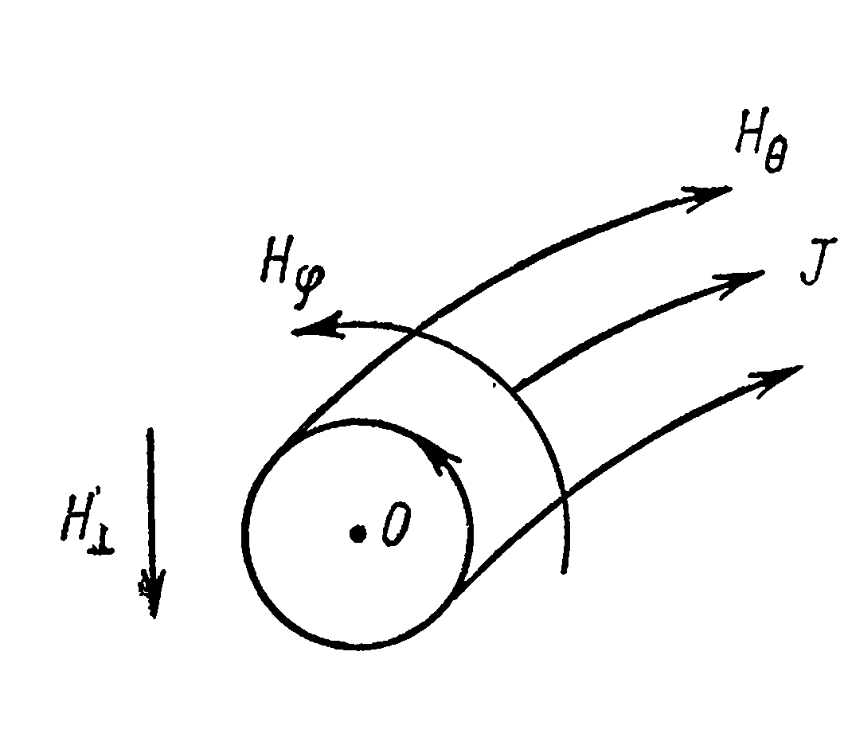
\includegraphics[width=0.5\linewidth]{6.tokamak_fields.png}
	\end{center}
    \caption{Поля в токамаке~\cite{arzimovich}}
    \label{fig:tokamak_fields} 
\end{figure}

Для равновесия плазмы в токамаке необходимо соответственно два условия равновесия: одно соответствует равновесию по малому радиусу тора $a$, и второе -- по большому радиусу $R$. Считая $a\ll R$, как это обычно бывает в реальных токамаках, условие равновесия по малому радиусу идентично условию равновесия бесконечно длинного плазменного шнура с радиусом $a$ (наличие аксиального поля $B_z$ принципиально не меняет условие равновесия):

\begin{equation*}
   \overline{p} + \frac{\overline{B_\theta^2}}{8\pi} = \frac{B_\theta(a)^2}{8\pi} + \frac{B_\varphi(a)^2}{8\pi},
\end{equation*}

где в левой части черта означает усреднение по сечению плазмы, а в правой части величины рассчитываются на границе плазмы (на радиусе $a$). По теореме Стокса полоидальное поле $B_\varphi$ можно выразить через полный ток $I$, текущий по плазменному кольцу:

\begin{align*}
   &2\pi a B_\varphi(a) = \frac{4\pi I}{c} \\
   &B_\varphi(a) = \frac{2I}{ac}
\end{align*}

Тогда получаем следующее уравнения равновесия:

\begin{equation*}
   2\pi a^2\overline{p} = \frac{I^2}{c^2} + \frac{a^2}{4}\left( B_\theta^2(a) - \overline	{B_\theta^2} \right)
\end{equation*}

Для определения равновесия по большому радиусу отдельно определим радиальные силы, действующие на тороидальный плазменный шнур. Всего имеется 3 различных источника радиальных сил:

\begin{enumerate}
	
   \item Расталкивающая сила, действующая на проводник с током. Сила, действующая на проводник, пропорциональна квадрату тока $I$ и зависит от его геометрии:
   
   \begin{equation*}
      f_1 = \frac{I^2}{2c^2} \pdv{\mathcal{L}}{R}
   \end{equation*}

   где $\mathcal{L}$ -- коэффициент самоиндукции. Он имеет размерность длины и, следовательно, $\partial\mathcal{L}/\partial R$ -- безразмерный коэффициент, зависящий от геометрии проводника. Для кольцевого витка:
   
   \begin{equation*}
      \pdv{\mathcal{L}}{R} = 2\pi \left( \ln\frac{b}{a} + l_i \right)
   \end{equation*}

   где $b>a$ -- радиус камеры токамака, $0<l_i<1/4$ -- внутренняя индуктивность плазмы. В любом случае $\partial\mathcal{L}/\partial R\sim 2\pi$.

   \item Расталкивание из-за давления плазмы. Сила такого расталкивания легко находится из следующего выражения:
   
   \begin{equation*}
      f_2 = \int\limits_{V} p \dv{V}{R} = \overline{p} \pi a^2 \dv{2\pi R}{R} = 2\pi^2 a^2 \overline{p}
   \end{equation*}

   \item ``Пондеромоторная'' сила из-за отличия напряжённости магнитного поля внутри и снаружи плазмы (из-за диамагнетизма). Строгий вывод я не понял, но по смыслу и размерности можно записать:
   
   \begin{equation*}
      f_3 = \frac{\pi a^2}{4}\left( B_\theta^2(a) - \overline{B_\theta^2} \right)
   \end{equation*}

\end{enumerate}

Для равновесия суммарная расталкивающая сила $f_1+f_2+f_3$ должна уравновешиваться силой, связанной с аксиальным полем $B_z$:

\begin{equation*}
   \frac{I^2}{2c^2} \pdv{\mathcal{L}}{R} + 2\pi^2 a^2 \overline{p} + \frac{\pi a^2}{4}\left( B_\theta^2(a) - \overline{B_\theta^2} \right) = \frac{2\pi R}{c} B_z I
\end{equation*}

Учитывая условие равновесия по малому радиусу тора, получаем итоговое уравнение равновесия плазмы в токамаке:

\begin{equation*}
   \frac{I^2}{c^2} \left( \frac{1}{2\pi}\pdv{\mathcal{L}}{R} - 1 \right) + 4\pi a^2 \overline{p} = \frac{2 R}{c} B_z I
\end{equation*}

\subsubsection{Физические механизмы нарушения равновесности плазмы}

Равновесие плазмы имеет условный
характер, так как оно с течением времени разрушается из-за диффузии и теплоотвода~\cite{arzimovich}.

Можно говорить о неизбежности \uline{диффузии} магнитного поля
внутрь объема, занимаемого плазмой, т. е. в область более слабого
поля. Таким образом, магнитное поле, вообще говоря, будет изменяться во времени. Но тогда давление плазмы тоже должно меняться, т. е. будет происходить изменение распределения
плазмы в пространстве. Этот встречный процесс также имеет диффузионный характер.

Уравнение, описывающее процесс диффузии плазмы в магнитном поле при $P\ll B^2/8\pi$, можно вывести следующим образом. Равновесие плазмы достигается в результате протекания тока плотностью

\begin{equation*}
	j = \frac{c}{B}\nabla P
\end{equation*}

Электрическое сопротивление
такому току есть следствие силы трения между электронами и ионами:

\begin{equation*}
	F = m_e\frac{j}{en}\nu_{ei},
\end{equation*}

где $\nu_{ei}$ -- частота электрон-ионных столкновений. Тогда под действием этой силы происходит дрейф со скоростью (см.~\eqref{eq:drift_common_eq}):

\begin{equation} \label{eq:magnetic_drift}
	\vb{u}_d = c \frac{m_e}{e^2H^2n}\nu_{ei}[\vb{j}\times\vb{B}],
\end{equation}

одинаковую для электронов и ионов. Подставим теперь найденную скорость $\vb{u}_d $ движения плазмы под действием сил трения в уравнение непрерывности. Получим уравнение
диффузии

\begin{equation*}
	\pdv{n}{t} = -div(n\vb{u}_d) \approx \frac{cnm_e\nu_{ei}}{e^2 B^2n}cT\Delta n = \frac{c^2P}{\sigma B^2} \Delta n
\end{equation*}

Итак, в реальном случае плазмы с конечной электропроводностью строгого равновесия не существует, так как скорость плазмы отлична от нуля. Это значит, что инерционный член в уравнении Эйлера, вообще говоря, не обращается в нуль и можно говорить лишь о приближенном выполнении условия равновесия.

Допустим, что $\tau_P$ -- характерное время, за которое происходит
изменение плотности плазмы. Тогда сделанное приближение справедливо при условии

\begin{equation*}
	\abs{\frac{nm_iu_d}{\tau_P}} \ll \frac{1}{c} \abs{[\vb{j}\times\vb{B}]}
\end{equation*}

Подставляя $\vb{u}_d$ из~\eqref{eq:magnetic_drift}, получаем

\begin{equation*}
	\frac{nm_i\frac{cm_e}{e^2B^2n}\nu_{ei}}{\tau_p}\ll\frac{1}{c}\leftrightarrow \frac{m_i c}{e B\tau_P} \ll \frac{eB}{m_ec}\frac{1}{\nu_{ei}} \leftrightarrow \frac{1}{\omega_{Bi}\tau_p}\ll\omega_{Be}\tau_{ei}
\end{equation*}

Отсюда видно, что чем выше степень замагниченности плазмы, тем
с больший правом можно говорить о ее равновесии.

Очевидно, что \uline{теплопроводность} плазмы в направлении, перпендикулярном к $B$, также должна резко снижаться при увеличении напряженности поля. В противоположность диффузии, которая обусловлена столкновениями между ионами и электронами, тепло- теплопередача в плазме поперек силовых линий происходит в основном в результате ион-ионных столкновений (если $T_i$ не слишком мало по сравнению с $T_e$). Это объясняется тем, что интенсивность теплопередачи зависят от ширины той области, в пределах которой при наличии градиента температуры перемешиваются траектории частиц с различной тепловой энергией. Коэффициент теплопроводности в направлении, перпендикулярном к $B$, пропорционален квадрату ширины области перемешивания, а эта ширина по порядку величины сравнима с ларморовским радиусом. Поэтому теплопередача в основном идет через ионную компоненту:

\begin{equation*}
	\chi\approx\frac{r^2_{L_i}}{\tau_H}
\end{equation*}

\subsection{Неустойчивость плазмы, виды неустойчивости, перегревная и ионизационная неустойчивости}

Плазма также может оказаться
\uline{неустойчивой} относительно малого отклонения от положения равновесия. Имеет смысл говорить лишь о таких неустойчивостях, которые разрушают равновесие плазмы за время меньшее, чем время диффузии.

Существенно, что различные механизмы нарушения равновесия допускают классификацию по скорости развития связанных с ними возмущений. Это позволяет ориентировать теорию на последовательное рассмотрение неустойчивостей и условий их стабилизации, начиная с тех, которые вызывают наиболее быстрые перемещения плазмы и поэтому являются самыми опасными (магнитогидродинамические). При возмущениях магнитогидродинамического типа макроскопические участки плазмы могут приобрести скорости порядка тепловой скорости ионов~\cite{arzimovich}. 

Другой подход: поскольку неустойчивость всегда представляет собой такое движение, которое уменьшает свободную энергию плазмы и переводит ее в состояние, более близкое к термодинамическому равновесию, то неустойчивости можно классифицировать в соответствии с видом свободной энергии, приводящей к их раскачке. Существует
четыре основных вида неустойчивостей~\cite{chen}.

\subsubsection{Виды неустойчивости}

\begin{itemize}
	
	\item потоковые неустойчивости -- в этом случае через плазму либо движется пучок частиц высокой энергии, либо протекает ток, вследствие чего частицы разных сортов движутся относительно друг друга. Энергия этого движения и используется для возбуждения волн; колебания усиливаются за счет запаса кинетической энергии, который имеется в начальном невозмущенном состоянии.
	
	\begin{itemize}
		
		\item Пример: \uline{двухпотоковая/бунемановская неустойчивость}. Рассмотрим холодную ($T_e=T_i=0$) однородную плазму с неподвижными ионами и электронами со скоростью $\vb{v}_0$. Магнитного поля нет. Тогда линеаризованные уравнения движения имеют вид [первый порядок малости]:
		
		\begin{align*}
			&Mn_0\pdv{\vb{v}_{i_1}}{t} = en_0\vb{E_1};\\
			&mn_0\left[\pdv{\vb{v}_{e_1}}{t}+(\vb{v}_0\cdot\nabla)\vb{v}_{e_1}\right] = -en_0\vb{E}_1.
		\end{align*}
	
		Пусть $\vb{E}_1 = E\vb{x}e^{i(kx-\omega t)}$, где ось $\vb{x}$ направлена по $\vb{v}_0$ и $\vb{k}$. Уравнения перепишутся в виде:
		
		\begin{align*}
			v_{i_1} &= i\frac{e}{M\omega}E;\\
			v_{e_1} &= -i\frac{e}{m(\omega-kv_0)}E.
		\end{align*}
	
		Рассмотрим уравнения непрерывности для электронов и ионов и подставим туда найденные выражения для скоростей:
		
		\begin{align*}
			&\pdv{n_{i_1}}{t} + n_0\div{\vb{v}_{i_1}} = 0;\\
			&\pdv{n_{e_1}}{t} + n_0\div{\vb{v}_{e_1}} + (v_0\cdot\nabla) n_{e_1} = 0.
		\end{align*}
	
		\begin{align*}
			n_{i_1} &= i\frac{en_0k}{M\omega^2}E;\\
			n_{e_1} &= -i\frac{en_0k}{m(\omega-kv_0)^2}E.
		\end{align*}
	
		И подставим их в уравнение Пуассона:
		
		\begin{align*}
			\div{\vb{E}_1} &= e(n_{i_1}-n_{e_1}) \\
			ik E &= e(ien_0kE) \left[ \frac{1}{M\omega^2} + \frac{1}{m(\omega - kv_0)^2}\right] 
		\end{align*}
		
		Получили дисперсионное биквадратное уравнение [с точностью до $4\pi$]:
		
		\begin{equation*}
			1 = \omega_p^2\left[\frac{m}{M\omega^2} + \frac{1}{(\omega - kv_0)^2}\right] 
		\end{equation*}
	
		Если ввести $x\equiv\frac{\omega}{\omega_p}$ и $y\equiv\frac{kv_0}{\omega_p}$, то можно переписать в виде:
		
		\begin{equation*}
			1 = \frac{m}{Mx^2}+\frac{1}{(x-y)^2} \equiv F(x, y)
		\end{equation*}
		 
		Существуют такие малые $y$, при которых зависимость $F(x,y)$ будет выглядеть так, как показано на рис.~\eqref{fig:two_stream_instability}. Всего два пересечения с прямой $y=1$ -- значит, есть два комплексно-сопряженных корня уравнения, один из которых даёт искомую неустойчивость.
		
		\begin{figure}[ht]
			\begin{center}
				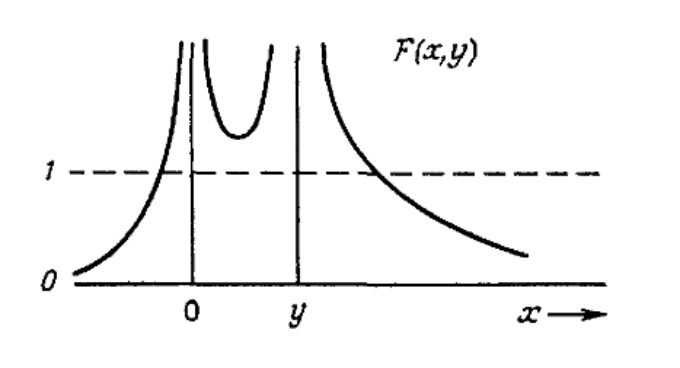
\includegraphics[width=0.5\linewidth]{two_stream_instability}
			\end{center}
			\caption{Функция $F(x,y)$ для двухпотоковой неустойчивости. Случай неустойчивой плазмы~\cite{chen}}
			\label{fig:two_stream_instability} 
		\end{figure}
		
		\uline{Смысл}: требование на малость $y\sim v_0$ возникло из заложенного в условии равенства $T=0$. В более честном подходе должно быть малое $v_0$, но больше тепловой скорости $v_0>v_T$, иначе доминирует эффект затухания Ландау (см.~\ref{subsubsec:Landau_damping}) и неустойчивости нет. Физический смысл неустойчивости: совпадение электронных и ионных плазменных частот колебаний из-за доплеровского сдвига.
		
	\end{itemize}

	\item неустойчивости Релея-Тэйлора -- в этом случае в плазме существует градиент плотности. Кроме того, к плазме должна быть приложена внешняя сила неэлектромагнитного характера, которая и вызывает неустойчивость. 
	
	\begin{itemize}
		
		\item Пример: \uline{гравитационная/Крускала—Шварцшильда неустойчивость}. Рассмотрим простейший пример такой неустойчивости (см. рис.~\ref{fig:gravity_instability_given}). Пусть плазма лежит в плоскости $yz$, градиент плотности $\nabla n_0$ ориентирован в направлении $-x$, а поле силы тяжести $\vb{g}$ -- по $x$. Для простоты будем считать, что $T_i=T_e=0$ и пусть магнитное давление существенно превышает давление плазмы.
		
		\begin{figure}[ht]
			\begin{center}
				\begin{minipage}[ht]{0.49\linewidth}
					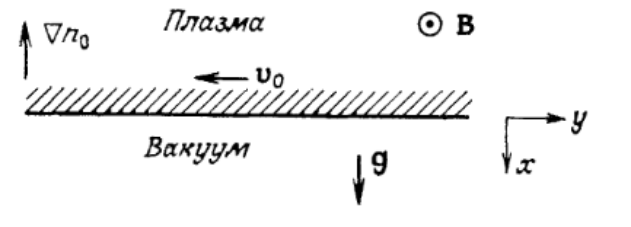
\includegraphics[width=1\linewidth]{gravity_instability_given}
					\caption{Гравитационная неустойчивость поверхности плазмы: дано~\cite{chen}}
					\label{fig:gravity_instability_given}
				\end{minipage}
				\hfill
				\begin{minipage}[ht]{0.49\linewidth}
					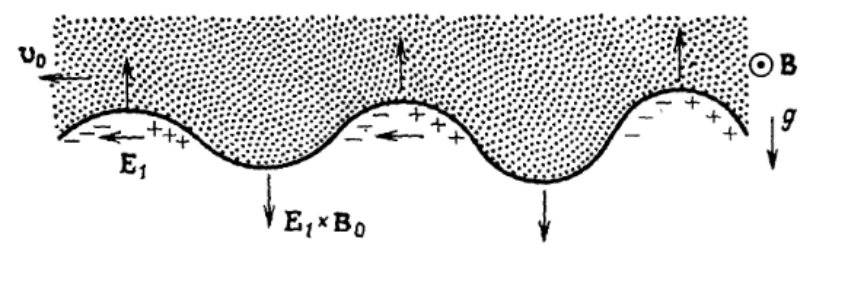
\includegraphics[width=1\linewidth]{gravity_instability_result}
					\caption{Гравитационная неустойчивость поверхности плазмы: результат~\cite{chen}}
					\label{fig:gravity_instability_result}
				\end{minipage}
			\end{center}
		\end{figure}
	
		Уравнение движения ионов имеет вид:
		
		\begin{equation*}
			Mn_0 (\vb{v}_0\cdot\nabla)\vb{v}_0 = en_0[\vb{v}_0\times\vb{B}]+Mn_0\vb{g}
		\end{equation*}
		
		Пусть $\vb{g}=const$, тогда член слева равен нулю. Умножим векторно на $B_0$ и получим:
		
		\begin{equation*}
			\vb{v}_0 = \frac{M}{eB_0^2}[\vb{g}\times\vb{B}] = \frac{g}{\omega_{Bi}}\vb{y}
		\end{equation*}
		
		В ответ явно входит знак заряда -- электроны двигаются в противоположную сторону, однако из-за массы в числителе их движением можно пренебречь. Тогда при возникновении на границе раздела ``ряби'' она будет нарастать из-за движения ионов. Возникает электрическое поле, которое имеет неоднородный
характер; если двигаться вдоль поверхности раздела, то при каждом переходе от горба к впадине электрическое поле меняет знак -- см. рис.~\ref{fig:gravity_instability_result}.
		
		Дисперсионное уравнение для этого случая будет иметь вид [без вывода]:
		
		\begin{equation*}
			\omega^2-kv_0\omega-g\frac{\partial n_0/\partial x}{n_0}=0
		\end{equation*}
	
		Условие на наличие неустойчивости:
		
		\begin{equation*}
			-g\frac{\partial n_0/\partial x}{n_0}>\frac{1}{4}k^2v_0^2
		\end{equation*}
	
		Для выполнения неравенства необходимо, чтобы у $g$ и $\frac{\partial n_0/\partial x}{n_0}$ были разные знаки -- т.е. чтобы более тяжёлая жидкость лежала ``на'' более лёгкой. Если вместо гравитационной силы рассматривается аналогичная центробежная сила в случае искривленных силовых линий магнитного поля, то устойчивость плазмы зависит от кривизны этих линий. Если силовые линии выгнуты
в сторону плазмы, то такая конфигурация устойчива. При достаточно малых $k$ инкремент неустойчивости даётся выражением:
		
		\begin{equation*}
			\gamma = Im(\omega) \approx [-g\frac{\partial n_0/\partial x}{n_0}]^{1/2}
		\end{equation*}
	
		Подобную неустойчивость колебаний границы плазмы с $\vb{k}\perp\vb{B}$ иногда называют \uline{желобковой}, потому что в плазменном цилиндре, когда все силы направлены по радиусу, эти волны распространяются в направлении $\theta$, а поверхности постоянной плотности напоминают рифлёные греческие колонны~\cite{chen}.	Если же параметр $\beta$ (отношение обычного и магнитного давлений) примерно равен 1, то могут возникать локальные неустойчивости в виде ``языков''~\cite{arzimovich}. 
		
		\uline{Смысл}: магнитное поле действует как легкая жидкость, удерживающая тяжелую плазму, поэтому возникает типичная гидродинамическая неустойчивость.
		
	\end{itemize}

	\item универсальные неустойчивости -- в этом случае плазма удерживается в ловушке. Даже при отсутствии сил, вызывающих ее движение, например электрических или гравитационных, плазма все равно не находится в полном термодинамическом равновесии. Давление плазмы стремится ее расширить, а связанная с этим процессом энергия может высвободиться в виде неустойчивости. Такого рода свободная энергия всегда присутствует в любой ограниченной плазме, поэтому подобные неустойчивости называются универсальными.
	
	\begin{itemize}
		
		\item Пример: \uline{возбуждение резистивной дрейфовой волны/дрейфовая неустойчивость}. Пусть волновой вектор $\vb{k}$ имеет компоненту вдоль магнитного поля $\vb{B}_0$.
		
		\begin{figure}[ht]
			\begin{center}
				\begin{minipage}[ht]{0.49\linewidth}
					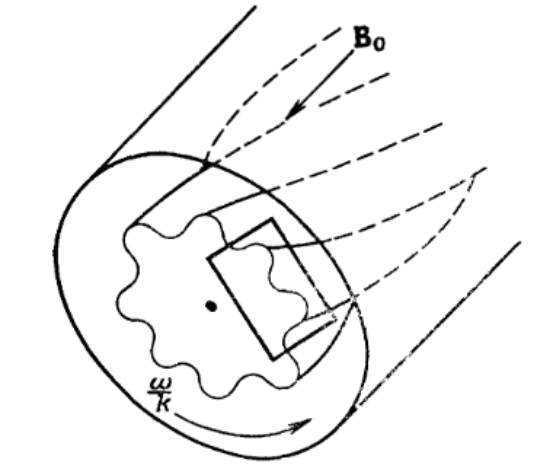
\includegraphics[height=0.25\textheight]{drift_instability_given}
					\caption{Дрейфовая неустойчивость поверхности плазмы: дано~\cite{chen}}
					\label{fig:drift_instability_given}
				\end{minipage}
				\hfill
				\begin{minipage}[ht]{0.49\linewidth}
					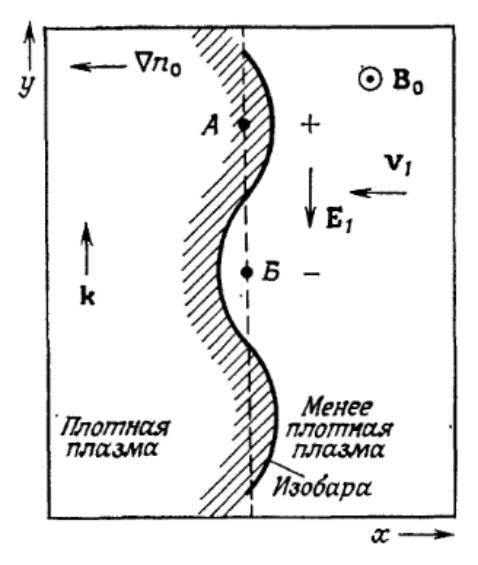
\includegraphics[height=0.25\textheight]{drift_instability_result}
					\caption{Дрейфовая неустойчивость поверхности плазмы: результат~\cite{chen}}
					\label{fig:drift_instability_result}
				\end{minipage}
			\end{center}
		\end{figure}
		
		Если увеличить участок поверхности, обведенный на рис.~\ref{fig:drift_instability_given} прямоугольником, и выпрямить его, то он будет выглядеть так, как показано на рис.~\ref{fig:drift_instability_result}. Единственная сила, которая может вызвать неустойчивость, -- это градиент давления $T\nabla n_0$ ($T=const$). В этом случае скорости дрейфовых движений в нулевом приближении по амплитуде волн записываются (при $E_0 = 0$) в виде:
		
		\begin{equation*}
			\vb{v}_{i_0} = \frac{T_i}{eB_0}\frac{\partial n_0/\partial x}{n_0}\vb{y};\;\vb{v}_{e_0} = \frac{T_e}{eB_0}\frac{\partial n_0/\partial x}{n_0}\vb{y}
		\end{equation*}
	
	 	Фазовая скорость дрейфовых волн приближенно равна $\vb{v}_{e_0}$. 
	 	
		Дрейфовые волны являются неустойчивыми, поскольку скорость ионов не равна в точности отношению полей: существуют поправки к этой величине, связанные с поляризационным дрейфом и дрейфом из-за неоднородности электрического поля. Под их влиянием распределение потенциала в дрейфовых колебаниях отстает по фазе от распределения плотности. Из-за этого сдвига скорость будет направлена из плазмы на тех участках, где плазма уже сдвинута наружу (и наоборот); поэтому возмущения в дрейфовых колебаниях будут нарастать. Если бы дополнительного фазового сдвига не было, то разность фаз составляла бы $\frac{\pi}{2}$, как показано на рис.~\ref{fig:drift_instability_result}, и дрейфовые волны были бы чисто осциллирующими.
		
		Дисперсионное уравнение для этого случая будет иметь вид [без вывода]:
		
		\begin{equation*}
			\omega^2+i\sigma_\parallel(\omega-\omega_{*})=0,
		\end{equation*}	
		
		где $\sigma_\parallel = \omega_{Bi}\frac{k_z^2}{k_y^2}\omega_{Be}\tau_{ei}$; $\omega_{*} = k_yv_{e_0}$.
		
		Условие на наличие неустойчивости:
		
		\begin{equation*}
			\sigma_\parallel \gg \omega,
		\end{equation*}
		
		тогда $\omega \approx \omega_{*} + i \frac{\omega_{*}^2}{\sigma_\parallel}$. Следовательно, 
		дрейфовые волны неустойчивы в любой плазме, имеющей градиент плотности. Cделав
поле $B_0$ неоднородным, ее развитие вообще можно остановить.
		
	\end{itemize}

	\item кинетические неустойчивости -- в этом случае распределение частиц плазмы по скоростям должно быть отлично от максвелловского (равновесного). Например, если $T_\parallel\neq T_\perp$, то может возникнуть неустойчивость, которая называется \uline{модифицированной неустойчивостью Харриса}. В пробкотронах [простых магнитных ловушках] из-за наличия конуса потерь существует дефицит частиц с большим отношением $v_\parallel/v_\perp$; эта анизотропия приводит к так называемой \uline{конусной неустойчивости}.
	
	\begin{itemize}
		
		\item Пример: \uline{неустойчивость Вейбеля}.  Пусть ионы покоятся, а температура электронов, движущихся вдоль оси $\vb{y}$, выше, чем при движении в $\vb{x}$ и $\vb{z}$ направлениях. В этом случае в плазме имеется избыток быстрых электронов, движущихся вдоль оси $\vb{y}$, однако вследствие того, что вверх движется столько же частиц, сколько и вниз, полный ток равен нулю (см. рис.~\ref{fig:weibel_instability}). Пусть из шумового фона спонтанно возникло распределение магнитного поля $\vb{B} = B_z\vb{z} \cos{kx}$. Тогда сила Лоренца искривит траектории электронов так, как это показано на рисунке штриховыми линиями, и в результате частицы, движущиеся вниз, будут собираться в слое А, а электроны, движущиеся вверх,— в слое Б. Возникающие при этом токовые слои будут сфазированы в точности таким образом, чтобы усилить возникшее вначале распределение магнитного поля, и возмущение $\vb{B}$ будет расти. Инкремент при этом равен $\gamma = \omega_p\frac{v_T}{c}$.
				
		\begin{figure}[ht]
			\begin{center}
				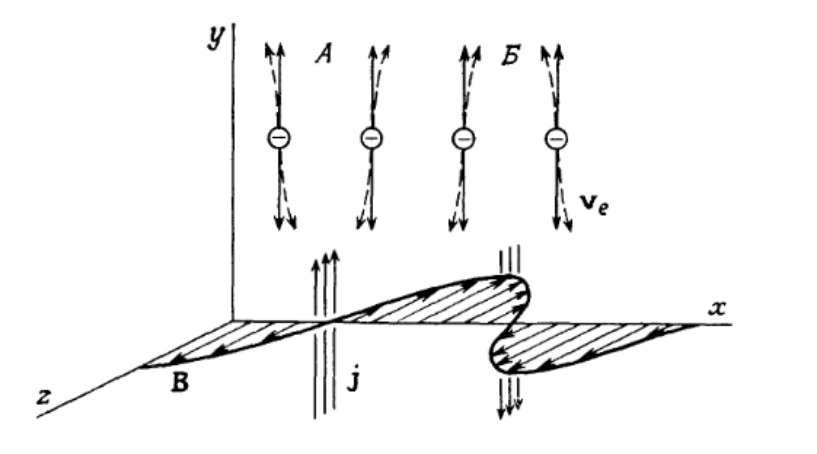
\includegraphics[width=0.5\linewidth]{weibel_instability}
			\end{center}
			\caption{Физический механизм неустойчивости Вейбеля~\cite{chen}}
			\label{fig:weibel_instability} 
		\end{figure}
		
		
	\end{itemize}

\end{itemize}

\subsubsection{Перегревная и ионизационная неустойчивости}

Плазма дугового разряда среднего давления [$10-200$ Торр], как правило, всегда неустойчива. В ней могут развиваться три вида гидродинамических неустойчивостей: ионизационная, акустическая и перегревная. Все эти виды неустойчивостей могут играть существенную роль в работе МГД-генераторов и плазмотронов~\cite{golubev}.

\uline{Ионизационная неустойчивость} характерна для изотермической плазмы, где имеется существенный отрыв температуры электронов от температуры газа. Наиболее ярко ее развитие проявляется для дуговых разрядов в присутствии внешнего магнитного поля, в частности, в МГД-генераторах при неравновесной проводимости, но она может развиваться в определенных условиях и без магнитного поля. Механизм такой неустойчивости, как и любых других, связан с появлением положительных обратных связей. Качественно его можно объяснить следующим образом. Джоулевая энергия $W=\sigma E^2$ , выделяемая в электронном газе, уравновешивается упругими $W_y$ и неупругими $W_{ny}$ потерями энергии электронами $\frac{T_e-T}{\tau_y}\delta n_e$. В плазме благодаря этому устанавливается определенная температура $T_e$ и концентрация $n_e$ электронов. Очевидно, если производная $\partial W/\partial (W_y+W_{ny})$, то возможен перегрев электронного газа, т.е. развитие ионизационной неустойчивости.
 
Нагреваемые электрическим полем электроны теряют свою энергию при упругих столкновениях с тяжелыми частицами, а также при возбуждении колебательных и электронных уровней молекул. Тушение возбужденных уровней происходит в основном при столкновениях с тяжелыми частицами, при этом энергия возбуждения переходит в поступательную энергию частиц. Электронные уровни могут опустошаться также за счет излучения. Очень распространен в дуговом разряде случай, когда эффективная температура возбужденных уровней отличается от поступательной температуры газа и даже становится близкой к температуре электронов. В этом случае в неупругих потерях энергии узким местом является тушение газом возбуждений, где, очевидно, поток энергии, вообще говоря, не зависит от концентрации электронов. Это обстоятельство сразу создает условия для развития ионизационной неустойчивости.
 
Повышение степени неравновесновесности среды за счет возбуждения колебательных и электронных уровней приводит к возникновению ионизационной неустойчивости плазмы. В случае достаточно быстрых процессов релаксации этих уровней, т.е. когда эффективная температура заселения уровней практически не отличается от температура газа, ионизационная неустойчивость как правило, не развивается~\cite{golubev}.

\uline{Перегревная неустойчивость} может развиваться как в изотермической ($T_e=T$), так и неизотермической плазме ($T_e>T$) при увеличении скорости тепловыделения в газе. При этом локальная плотность газа при условии постоянства давления падает, падает частота соударений электронов с нейтральными частицами, проводимость плазмы растет. Рост проводимости приводит к локальному увеличению плотности тока и усилению неоднородности. Плазма с током практически всегда подвержена тепловой контракции~\cite{golubev}.

В случае слабоионизированной присадки или когда присадка отсутствует, заметное (на порядок) увеличение инкремента перегревной
неустойчивости происходит за счет ионизационного усиления неоднородности при повышении температуры электронов. В этом случае
перегревную неустойчивость часто называют \uline{ионизационно-перегревной}~\cite{golubev}.
 
\subsection{Энергетический принцип МГД-устойчивости}

\uline{Применимость}: Энергетический принцип неустойчивости плазмы, формально выводимый ниже из уравнений МГД, имеет разумный
смысл и для разреженной плазмы в дрейфовом приближении, так
как для наиболее опасных [``подозрительных''] возмущений (смещение $\vb{\xi}\perp\vb{B}$) движение происходит поперек силовых линий.

Введем бесконечно малое смещение $\vb{\xi}(\vb{r}, t)$ элемента, объема плазмы из положения равновесия, при этом $\vb{u}=\pdv{\vb{\xi}}{t}$. Оказывается, что линеаризованные уравнения общей теории устойчивости идеально проводящей плазмы можно привести к одному векторному уравнению~\cite{arzimovich}:

\begin{equation*}
	\pdv[2]{\vb{\xi}}{t}=-\hat{K}\vb{\xi},
\end{equation*}

где $\hat{K}$ -- некоторый дифференциальный оператор, действующий на $\xi$ как на функцию координат. Говоря формально, данное уравнение аналогично уравнению, описывающему колебания произвольной неоднородной упругой среды, где $\hat{K}$ играет роль соответствующего обобщенного коэффициента упругости. Перейдём в линеаризованных уравнениях МГД от переменной $\vb{u}$ к переменной $\vb{\xi}$. Рассмотрим~\eqref{eq:MGD_motion_eq} [перейдём к другим обозначениям]:

\begin{align*}
	n M \dv{\vb{u}}{t} &= \frac{1}{c}[\vb{j}\times\vb{B}]-\grad{(P_i+P_e)} \\
	\rho_0 \vb{\ddot{\xi}} &= \frac{1}{4\pi}([[\curl{\delta\vb{B}}]\times\vb{B}_0] + [[\curl{\vb{B_0}}]\times\delta\vb{B}])-\nabla \delta P
\end{align*}

С учётом уравнения непрерывности последнее слагаемое перепишется как:

\begin{equation*}
	-\nabla \delta P = -\nabla \left(\dv{P}{\rho}\delta\rho\right) = \nabla\left(\dv{P}{\rho}\div{\rho_0\xi}\right) = \nabla \left(\left(\dv{P}{\rho}\right) (\rho_0\div{\xi}+\xi\grad{\rho_0})\right) = \nabla(\gamma P\div{\xi}+\xi\grad{P})  
\end{equation*}

В итоге получаем (опуская индекс $0$):

\begin{equation*}
	\rho \vb{\ddot{\xi}}=\hat{F}\left\lbrace\xi\right\rbrace,
\end{equation*}

\begin{equation} \label{eq:elastic_coeff}
	\hat{F}\left\lbrace\xi\right\rbrace = \nabla(\gamma P\div{\xi}+\xi\grad{P}) + \frac{1}{c}[\vb{j}\times\curl{[\vb{\xi}\times\vb{B}]}]-\frac{1}{4\pi}[\vb{B}\times\curl{[\curl{\vb{\xi}\times\vb{B}}]}]
\end{equation}

По аналогии с механикой упругих сред естественно ввести в рассмотрение
потенциальную энергию малых колебаний $\delta W = \frac{1}{2}\int\xi\hat{K}\vb{\xi}\dd{V}$.

Если $\delta W>0$ для всех $\xi\neq0$, то отклонения от положения равновесия не могут нарастать во времени и, следовательно, плазма магнитогидродинамически устойчива. В противном случае, когда $\delta W$ может принимать отрицательные значения, коэффициент упругости отрицателен по отношению к некоторым деформациям, и, следовательно, рассматриваемая система неустойчива. Границу между устойчивыми и неустойчивыми конфигурациями образуют такие состояния, в которых исчезает упругость по отношению к одному определенному типу смещений. В этом случае наряду с исходным равновесным состоянием существуют близкие к нему равновесные состояния, соответствующие смещению $\xi$ в направлении упругости, равной нулю. Таким образом, для нахождения границы устойчивости достаточно определить, при каких условиях появляются близкие равновесные состояния, т. е. достаточно исследовать уравнение $\hat{F}\xi = 0$.

В выражении для потенциальной энергии $\delta W$ два слагаемых (см. два последних члена в~\eqref{eq:elastic_coeff}). Первое описывает изменение внутренней тепловой энергии плазмы, второе -- изменение магнитной энергии при перестройке конфигурации. Например, желобковая неустойчивость типа связана с высвобождением внутренней энергии плазмы (при расширении). При таких смещениях силовые линии магнитного поля не ``растягиваются'' и не ``изгибаются'', на что пришлось бы затрачивать энергию (это второе слагаемое в~\eqref{eq:elastic_coeff}).

\section{Колебания и волны в плазме}

\subsection{Основные типы колебания и волн в плазме: лэнгмюровские электонные и ионные, электромагнитные, ионно-звуковые, магнитозвуковые, альфвеновские}

В системе связанных осцилляторов с таким большим числом степеней свободы, как плазма, имеется много всевозможных типов колебаний; в плазме могут распространяться волнообразные возмущения, например, электрического поля $\vb{E}=\vb{E}_0exp[i(\vb{k}\vb{x}-\omega t)]$. Частота $\omega$ и волновое число $\vb{k}$ таких колебаний связаны дисперсионным уравнением, получаемым из уравнений движения плазмы. Фазовая скорость волны равна $v_{ph}=\omega/k$, а групповая скорость $v_{gr}=\partial\omega/\partial k$. В плазме могут распространяться как линейные (малой амплитуды), так и нелинейные волны (+ ударные волны)~\cite{kroll}.

\subsubsection{Лэнгмюровские колебания}



\subsubsection{Электромагнитные}

В диэлектрической среде однородные плоские электромагнитные волны распространяются с дисперсией, определяемой уравнением 

\begin{equation*}
	k^2=\frac{\omega^2\varepsilon}{c^2}
\end{equation*}

Диэлектрическая проницаемость холодной однородной и изотропной плазмы, состоящей из подвижных электронов и неподвижных ионов, на высоких частотах имеет вид:

\begin{equation*}
	\varepsilon = 1-\frac{\omega_{pe}^2}{\omega^2}
\end{equation*}

Соответствующее дисперсионное уравнение для \uline{электромагнитных} волн в плазме запишется следующим образом:

\begin{equation*}
	k^2 = \frac{\omega^2-\omega_{pe}^2}{den}
\end{equation*}

Если частота волн $\omega$ меньше плазменной частоты $\omega_{pe}$, то волновой вектор чисто мнимый. Волны с частотами выше плазменной распространяются в плазме; при очень высоких частотах свободные электроны плазмы оказывают лишь слабое влияние на электромагнитную волну. На распространение волн существенное влияние оказывают конечные размеры, постоянное магнитное поле или неоднородности плазмы~\cite{kroll}.

\subsubsection{Ионно-звуковые}

Звуковые волны в идеальном газе -- это продольные волны без  дисперсии, частота которых меньше частоты столкновений и которые  распространяются со скоростью звука $V_s=\sqrt{\gamma\frac{T}{m}}$, где $\gamma$ -- показатель адиабаты. В плазме также могут  распространяться низкочастотные акустические, или \uline{ионно-звуковые}, волны.  Возникающее в них из-за разделения зарядов поле согласует движение ионов и электронов. Скорость распространения таких волн:

\begin{equation*}
	c_s = \sqrt{\frac{Z\gamma_eT_e+\gamma_iT_i}{m_i}},
\end{equation*}

где $Z$ -- зарядовое число ионов. В отличие от звука в обычном газе ионно-звуковые волны слабо затухают лишь тогда, когда их частота много больше частоты столкновений, а температура электронов значительно превышает температуру ионов. При выполнении указанных выше условий такие продольные волны распространяются как акустические. В этом волновом движении инерция определяется ионами, а возвращающая сила электронным давлением~\cite{kroll}.

\subsubsection{Магнитозвуковые}



\subsubsection{Альфвеновские}

В плазме, находящейся в однородном постоянном магнитном поле, могут существовать многие другие волны. Например, при частотах ниже ионной циклотронной частоты в плазме распространяется медленная  электромагнитная волна без дисперсии (магнитогидродинамическая волна), называемая \uline{альфвеновской}, со скоростью 

\begin{equation*}
	V_A = \frac{B}{4\pi\rho_m},
\end{equation*}

где $\rho_m$ = $nm_i$ -- массовая плотность.

Кроме того, в неоднородной плазме распространяются \uline{дрейфовые} волны, обусловленные дрейфом частиц и возникновением токов, связанных с  градиентами плотности. Дополнительная степень свободы, возникающая  благодаря градиенту плотности, способствует образованию нового типа волн, распространяющихся с частотой~\cite{kroll} 

\begin{equation*}
	\omega\approx\frac{T}{m}\frac{1}{\omega_c}\frac{\grad{n}}{n}k
\end{equation*}

\subsubsection{Вистлеры}

Они же -- геликоны, свистящие атмосферики. НЧ (низкочастотные) волны в плазме в магнитном поле. Встречаются в ионосфере Земли, но теперь представляют интерес и в вопросе прикладного использования.

Групповая скорость этих волн близка к скорости света в вакууме, а их источником являются атмосферные электрические разряды (молнии). Атмосферики обладают слабым затуханием и могут распространяться на значительные расстояния. 

Рассматривается формула Эпплтона-Хартри для показателя преломления (см.~\ref{subsec:refractive_index}), выведенная в разделе~\ref{subsec:cold_magentic_plasma_waves} ($v=\frac{\omega_{pe}^2}{\omega^2}$ и $u=\frac{\omega_{Be}^2}{\omega^2}$, $o, e$ -- обыкновенная и необыкновенная волны соответственно):

\begin{equation*}
	n_{o,e}^2=1-\frac{2v(1-v)}{2(1-v)-u\sin^2\theta \pm \sqrt{u^2 \sin^4\theta+4u(1-v)^2 \cos^2\theta}}
\end{equation*}

Пусть $\omega_{pe}^2\gg\omega_{Be}^2$, т.е. $v\gg u \gg 1$. Тогда формула перепишется в виде:

\begin{align*}
	n_{o,e}^2&=1-\frac{2v(-v)}{2(-v)\pm\sqrt{4uv^2 \cos^2\theta}} \\
	n_{o,e}^2&=1+\frac{v^2}{-v\pm v\abs{\cos\theta}\sqrt{u}} \\
	n_{o,e}^2&=\pm \frac{v}{\sqrt{u}\abs{\cos\theta}} \\
	\frac{c^2k^2}{\omega^2} &= \pm\frac{\omega_{pe}^2}{\omega_{Be} \omega\abs{\cos\theta}} \\ 
	\omega &=\frac{k^2c^2\omega_{Be}}{\omega_{pe}^2}\abs{\cos\theta}
\end{align*}

Тогда групповая скорость вистлеров растёт с $k$:

\begin{equation*}
	v_{gr} = \pdv{\omega}{k} = \frac{2kc^2\omega_{Be}}{\omega_{pe}^2}\abs{\cos\theta}
\end{equation*}

При выборе конкретного $\theta$ получаем дисперсионную кривую $\omega(k)$ и чем при больших $k$ (т.е. правее) на ней находится частота рассматриваемой геликонной волны, тем быстрее эта волна прибежит к приёмнику (это в случае исследования вистлеров в ионосфере актуально). Можно перейти от угла к волновым векторам: 

\begin{equation*}
	\omega = \frac{k^2c^2\omega_{Be}}{\omega_{pe}^2} \frac{k_z}{\sqrt{k_y^2+k_z^2}} = \frac{c^2\omega_{Be}}{\omega_{pe}^2}k_z\sqrt{k_y^2+k_z^2}
\end{equation*}

Существует теорема Стори про вистлеры: самый большой угол между $\vb{v}_{gr}$ и $\vb{B}$ равен \uline{углу Стори}: $19.5^\circ$.

\subsubsection{Old version}

В изотропной плазме легко записать дисперсионное уравнение:

\begin{equation}
    \left(1-\frac{\omega^2}{c^2 k^2} \varepsilon_{\perp}\right) E_{\perp} + \varepsilon_{\parallel} E_{\parallel}= 0
\end{equation}

Найдём $\varepsilon$ для плазмы с Максвелловской функцией распределения по теории возмущений:

\begin{align*}
	& f = f_{T_e} + \delta f \\
	& \delta f \ll f_{T_e} \\
	\pdv{\delta f}{t} + v\pdv{\delta f}{x} = \frac{e}{m}E \pdv{f_{T_e}}{v}
\end{align*}

где $f_{T_e}$ -- максвелловская функция распределения с температурой $T_e$ и мы предположили, что $\vb{v} \parallel \vb{E}$. Рассмотрим $\exp{-i\omega t + i \vb{kr}}$ процесс, тогда:

\begin{equation*}
	\delta f = \frac{e}{m}\pdv{f_{T_e}}{v}\text{Re}\frac{Ee^{-i\omega t + i \vb{kr}}}{i\left( kv - \omega \right)}
\end{equation*}

Плотность тока $\vb{j}$ вычисляется через первый момент $\delta f$:

\begin{equation*}
	j = -e\int\limits_{-\infty}^{+\infty} v\delta f\dd v = \sigma E
\end{equation*}

Через связь $\varepsilon = 1 - 4\pi\sigma/i\omega$ находим:

\begin{equation*}
	\varepsilon = 1 + \frac{4\pi e^2}{m}\int\limits_{-\infty}^{+\infty}\frac{v }{\omega\left( \omega - kv \right)}\pdv{f_{T_e}}{v}\dd v
\end{equation*}

В числителе добавим и вычтем $\omega/k$:

\begin{equation*}
	\varepsilon = 1 + \frac{4\pi e^2}{mk}\int\limits_{-\infty}^{+\infty}\frac{kv - \omega }{\omega\left( \omega - kv \right)}\pdv{f_{T_e}}{v}\dd v + \frac{4\pi e^2}{mk}\int\limits_{-\infty}^{+\infty}\frac{1}{\left( \omega - kv \right)}\pdv{f_{T_e}}{v}\dd v
\end{equation*}

Второе слагаемое зануляется при подстановке на $\pm\infty$:

\begin{equation*}
	\varepsilon = 1 + \frac{4\pi e^2}{mk}\int\limits_{-\infty}^{+\infty}\frac{1}{\left( \omega - kv \right)}\pdv{f_{T_e}}{v}\dd v
\end{equation*}

Вообще говоря, делая этот вывод, мы работали с комплексными числами и интеграл в выражении выше берётся как интеграл по контуру в комплексной плоскости. С таким простым выводом нам, однако, неизвестно правило обхода возможных полюсов в знаменателе (при наличии затухания). Математически строго правило обхода полюсов выводится при применении преобразования Лапласа к функции распределения $f$ (а не Фурье, как сделали мы). Однако, физические соображения могут подсказать это правило. Мы ожидаем, что волны не могу произвольно самовозбуждаться в среде, но могут затухать, поэтому мнимая часть $\omega$ отрицательна:

\begin{equation*}
	\varepsilon = 1 + \frac{4\pi e^2}{mk}\int\limits_{-\infty}^{+\infty}\frac{1}{\left( \omega - kv - i\nu\right)}\pdv{f_{T_e}}{v}\dd v
\end{equation*}

В таком случае обходить полюс надо снизу (см. Рис.~\ref{fig.7.pole}). В итоге можно переписать:

\begin{equation*}
	\varepsilon = 1 + \frac{4\pi e^2}{mk}\dashint\frac{1}{\left( \omega - kv \right)}\pdv{f_{T_e}}{v}\dd v - i\frac{4\pi^2 e^2}{mk}\int\limits_{-\infty}^{\infty}\delta\left( \omega - kv \right)\pdv{f_{T_e}}{v}\dd v
\end{equation*}

где второе слагаемое -- это интеграл в смысле главного значения, а третье -- полувычет.

\begin{figure}[ht]
	\label{fig.7.pole} 
	\begin{center}
		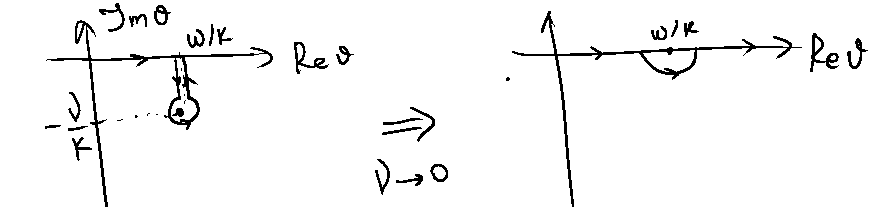
\includegraphics[width=1\linewidth]{7.pole.pdf}
	\end{center}
	\caption{Пояснение правила обхода}
\end{figure}

Запишем теперь это выражения явно для максвелловской функции распределения:

\begin{align*}
	& f_{T_e} = \frac{N}{v_T\sqrt{2\pi}} e^{-v^2/2 v_T^2} \\
	& \pdv{f_{T_e}}{v} = -\frac{Nv}{v_T^3 \sqrt{2\pi}}e^{-v^2/ 2 v_T^2} \\
	& \varepsilon = 1 - \frac{\omega_p^2}{v_T^3 k^2\sqrt{2\pi}}\int\limits_{-\infty}^{+\infty}\frac{kv + \omega - \omega }{\omega - kv} e^{-v^2/ 2 v_T^2} \dd v = \\
	&= 1 + \frac{\omega_p^2}{k^2 v_T^2} \left( 1 - \frac{z}{\sqrt{\pi}}\int\limits_{-\infty}^{+\infty}\frac{e^{-y^2}}{z-y}\dd y \right)
\end{align*} 

где $z = \omega/\sqrt{2}kv_T = v_{ph}/\sqrt{2}v_T$. Предполагая, что $\text{Im}\,z\ll 1$, т.е. $\text{Im}\omega \ll kv_t$ считаем, что полюс лежит на действительной оси, т.е.:

\begin{equation*}
	\int\limits_{-\infty}^{+\infty}\frac{e^{-y^2}}{z-y}\dd y = -i\pi e^{-z^2} + \dashint\frac{e^{-y^2}}{z-y}\dd y
\end{equation*}

В предельных случаях можно вычислить дальше:

\begin{enumerate}
	\item $|z| \gg 1$ ($\omega \gg kv_T$):
	
	Раскладываем:
	
	\begin{align*}
		\frac{1}{z-y} = \frac{1}{z} + \frac{y}{z^2} + \frac{y^2}{z^3} + \dots
	\end{align*}

	Слагаемые с нечётной степенью $y$ зануляются, т.к. в таком случае под интегралом нечётная функция. Также мнимая часть пропадает, т.к. $\exp{-z^2}\rightarrow 0$. В таком случае дисперсионка имеет вид:
	
	\begin{align*}
		\varepsilon = 1 + \frac{\omega_p^2}{k^2 v_T^2} \left( 1 - \frac{z}{\sqrt{\pi}}\left( \frac{\sqrt{\pi}}{z} + \frac{\sqrt{\pi}}{2z^3} + \frac{3\sqrt{\pi}}{4z^5} + \dots \right) \right) \\
		=1 - \frac{\omega_p^2}{\omega^2}\left( 1 + 3\frac{k^2 v_T^2}{\omega^2} + \dots \right)
	\end{align*}

	Отсюда видно, что плазменные волны на самом деле имеют ненулевую фазовую скорость.
	
	\item $|z| \ll 1$ ($\omega \ll kv_T$):
	
	В интеграле в смысле главного значения считаем $z=0$, тогда интеграл равен нулю, т.к. функция нечётная (его формальная расходимость нас не пугает, т.к. это интеграл в смысле главного значения). Тогда остаётся только вычет:
	
	\begin{align*}
		\varepsilon = 1 + \frac{\omega_p^2}{k^2 v_T^2} \left( 1 - i \frac{\omega}{k v_T}\sqrt{\frac{\pi}{2}}e^{-\omega^2/2k^2v_T^2} \right)
	\end{align*}

	Таким образом продольные плазменные волны (Ленгмюровские) затухают при больших $k$.
	
\end{enumerate}

Теперь найдём дисперсионки исходя из найденного $\varepsilon$. Из условия $\varepsilon_{\parallel} = 0$ получаем первый тип волн - продольные(ленгмюровские/электростатические) 
волны. Затухание Ландау(безстолкновительное затухание) относится именно к таким волнам. Их дисперсионка имеет следующий
вид:

\begin{equation}
    \omega^2=\omega_p^2 + 3 (k v_{T})^2
\end{equation}

волны с частотой сильно отличной от плазменной затухают.

В случае $1 - \frac{\omega^2}{c^2 k^2} \varepsilon_{\parallel}=0$ получаем поперечные волны(почти как в вакууме). Для них
дисперсионка:

\begin{equation}
    \omega^2=\omega_p^2 + (c k)^2
\end{equation}

Легко видеть, что волны с частотой $\omega < \omega_p$ не распространяются.

Возможен случай, когда $v_{T_i} \ll \omega/k \ll v_{T_e}$. Тогда можно записать:

\begin{equation}
    \varepsilon=1+\frac{\omega_{pe}^2}{k^2 v_{Te}^2} - \frac{\omega_{pi}^2}{\omega^2}-3\frac{\omega_{pi}^2 k^2 v_{Ti}^2}{\omega^4}
\end{equation}

В случае низких частот (где влияние ионов существенно) можно пренебречь 4ым слагаемым, тогда дисперсионка примет следующий вид:

\begin{equation}
    \omega=\frac{k c_s}{\sqrt{1 + k^2 r_d^2}}
\end{equation}

при малых $k$ имеем $\omega=k c_s$, где $c_s=\frac{T_i + T_e}{M}$ (ионный звук). При больших частотах имеем ионные ленгмюровские волны (сильно затухают, если температура ионов не мала). Грубо дисперсионные соотношения для разных волн изоражены на рисунке~\ref{fig:disp_eq_without_B}.

\begin{figure}[ht]
	\begin{center}
		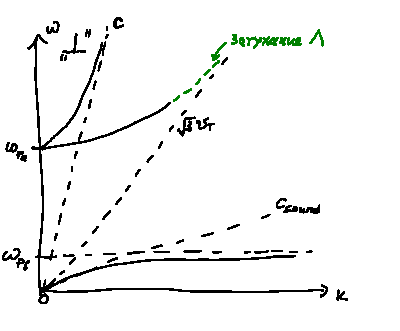
\includegraphics[width=85mm]{noB.pdf}
	\end{center}
	\caption{Дисперсионка для волн в плазме в отсутствии магнитного поля}
	\label{fig:disp_eq_without_B} 
\end{figure}

Альфвеновские волны. При рассмотрении предыдущих волн, движением ионов пренебрегалось. Рассматриваем случай, когда волна распространяется вдоль внешнего магнитного поля; также рассматриваются низкие частоты (сравнимые с циклотронной частотой ионов ?). Дисперсионка таких волн имеет следующий вид:

\begin{equation}
    \frac{\omega}{k}=\frac{B_0}{\sqrt{4\pi \rho}}
\end{equation}

где $\rho$ есть массовая плотность плазмы (все частицы). Важно, что фазовая скорость не зависит от частоты! По сути это совместное движение/осцилляции ионов и магнитных силовых линий поперек движения волны. Они распространяются без дисперсии.

Диэлектрическая проницаемость в холодной плазме с учетом ионов:

\begin{equation}
	\varepsilon=1 - \frac{\omega_{pe}^2}{\omega^2} - \frac{\omega_{pi}^2}{\omega^2},
\end{equation}

если есть столкновения (пусть отбросим ионы), то $\varepsilon=1-\frac{\omega_{pe}^2}{\omega (\omega+i \nu)}$. когда есть некоторый поток, движущийся со скоростью $\upsilon_0$, то без учета ионов и столкновений, имеем: $\varepsilon=1-\frac{\omega_{pe}^2}{(\omega - k \upsilon_0)^2}$.
Для затухания Ландау: $\varepsilon=1+\frac{4\pi e^2}{m} \int \frac{v}{\omega} \frac{\partial f_0}{\partial v} \frac{dv}{\omega-vk}$.

При наличии внешнего магнитного поля $B_0$ диэлектрическая проницаемость перестает быть изотропной(считаем, что трения нет и $\upsilon_T \ll \upsilon_{ph}$):

\begin{equation}
	\varepsilon=
	\begin{pmatrix}
		\varepsilon_B & ig & 0 \\
		-ig & \varepsilon_B & 0 \\
		0 & 0 & \varepsilon_{\parallel}
	\end{pmatrix}
\end{equation}
где $\varepsilon_B=1-\frac{\omega_{pe}^2}{\omega^2-\omega_{Be}^2}-\frac{\omega_{pi}^2}{\omega^2-\omega_{Bi^2}}$ и $g=\frac{\omega_{pe}^2 \omega_{Be}}{\omega (\omega^2-\omega_{Be}^2} -\frac{\omega_{pe}^2 \omega_{Be}}{\omega (\omega^2-\omega_{Be}^2}$, $\varepsilon_{\parallel}=1-\frac{\omega_{pe}^2}{\omega^2}-\frac{\omega_{pe}^2}{\omega^2}$. 

\subsection{Показатель преломления плазмы, пространственная и временная дисперсии, фазовая и групповая скорости плазменных волн}
\label{subsec:refractive_index}

\uline{Показатель преломления плазмы}

\begin{equation*}
	n = \frac{ck}{\omega} = \frac{k}{k_0} = \sqrt{\varepsilon}
\end{equation*}

Мнимая часть показателя преломления связана с поглощением среды.

\uline{Пространственная и временная дисперсия}. В общем случае электрическая индукция $\vb{D}$ зависит от напряжённости поля $\vb{E}$ нелинейным образом:

\begin{equation*}
    \vb{D}(\vb{r}, t) = \int\limits_{-\infty}^{t}\dd{t'} \int\limits_{\infty}\dd[3]{r'}\varepsilon(t, t',\vb{r},\vb{r}') \vb{E}(\vb{r}', t'),
\end{equation*}

\uline{Физический смысл}: временная дисперсия -- влияние среды немгновенное, среда ``помнит''; пространственная дисперсия из-за интеграла по всему пространству -- по сути, связана с тепловым движением частиц плазмы.

Для стационарной среды зависимость от времени имеет вид $t,\,t'\Rightarrow t-t'$ [масштаб временной дисперсии]; для однородной среды зависимость от координаты имеет вид $\vb{r},\,\vb{r}'\Rightarrow \vb{r}-\vb{r}'$ [масштаб пространственной дисперсии].

Можно всё раскладывать в интегралы Фурье\Tokman:

\begin{equation*}
	\forall \vb{A}(\vb{r},t)\Rightarrow \vb{A}(\vb{r},t)=\int\limits_{\infty}\dd{\omega} \int\limits_{\infty}\dd[3]{k}e^{-i\omega t+i\vb{k}\vb{r}}\vb{A}(\vb{k},\omega)
\end{equation*}

Если ввести обозначения $\tau=t-t'$ и $\vb{\varkappa} = \vb{r}-\vb{r}'$, то

\begin{equation*}
	\vb{D}(\vb{r}, t) = \int\limits_{\infty} \dd{\omega} \int\limits_{\infty} \dd[3]{k} \int\limits_{\infty} \dd{\tau} \int\limits_{\infty} \dd[3]{\varkappa} \varepsilon(t, \vb{\varkappa}) \vb{E}(\vb{k}, \omega) e^{-i\omega t+ i\vb{\varkappa}\vb{r}},
\end{equation*}

откуда

\begin{equation*}
	D_i(\omega, \vb{k}) = \varepsilon_{ij} (\omega, \vb{k}) E_j(\omega, \vb{k}),
\end{equation*}

где

\begin{equation*}
	\varepsilon_{ij} (\omega, \vb{k}) = \int\limits_0^\infty \dd{\tau}\int\limits_\infty\dd[3]{\varkappa}\varepsilon_{ij}(\tau,\vb{\varkappa})e^{-i\omega t+ i\vb{\varkappa}\vb{r}}.
\end{equation*}

Собственно, зависимость диэлектрической проницаемости от волнового вектора часто и называют \uline{пространственной дисперсией}, а от частоты -- \uline{временной дисперсией}. В таком случае линейная задача сводится к рассмотрению одной гармоники. Нахождение монохроматического отклика даёт тензор диэлектрической проницаемости $\varepsilon_{ij} (\omega, \vb{k})$.

Отсутствие пространственной дисперсии, изотропная плазма: $\varepsilon_{ij} = \varepsilon(\omega)\delta_{ij}$. 

Если добавим пространственную дисперсию, то:

\begin{equation*}
	\varepsilon_{ij} = \varepsilon_1 (\omega, \vb{k})\delta_{ij}+\frac{k_ik_j}{k^2}\varepsilon_2(\omega, \vb{k}) \Rightarrow \vb{D} = \varepsilon_1\vb{E}+\frac{\vb{k}(\vb{k}\vb{E})}{k^2}\varepsilon_2
\end{equation*}

Поскольку при $\vb{E}\perp\vb{k}$ $\vb{D} = \varepsilon_1\vb{E}$, то $\varepsilon_1=\varepsilon_{\perp}$. Аналогично $\varepsilon_2 = \varepsilon_{\parallel}-\varepsilon_1$.

Тогда \uline{диэлектрическая проницаемость изотропной плазмы}:

\begin{equation*}
	\varepsilon_{ij} = \varepsilon_\perp (\omega, \vb{k})\left( \delta_{ij}-\frac{k_ik_j}{k^2}\right) + \varepsilon_\parallel(\omega, \vb{k})\frac{k_ik_j}{k^2}
\end{equation*}

Масштаб пространственной дисперсии [без вывода]\Tokman:

\begin{equation*}
	\mu = \frac{\vb{B}}{\vb{H}} = \frac{1}{1-\frac{\omega^2}{c^2k^2}(\varepsilon_\perp-\varepsilon_\parallel)}
\end{equation*}

Если нет поглощения, то: $\varepsilon_{ij}(\omega, \vb{k})=\varepsilon_{ji}^{*}(\omega, \vb{k})=\varepsilon_{ij}^{*}(-\omega, -\overrightarrow{k})$\Tokman.

\uline{Фазовая и групповая скорости плазменных волн}

Фазовая скорость волны равна $v_{ph} = \omega/k$,
а групповая скорость $v_{gr} = \partial\omega/\partial k$.

Пример изображения фазовых скоростей -- см. рис.~\ref{fig:disp_eq_without_B}.

Фазовая скорость может быть больше скорости света (но это не страшно, т.к. она не является скоростью передачи информации и нет на самом деле ограничения на её величину).

\section{Взаимодействие заряженных частиц с волнами в плазме}
 
\subsection{Возбуждение и затухание волн в плазме, черенковское излучение, затухание Ландау}

\subsubsection{Затухание Ландау}
\label{subsubsec:Landau_damping}

\subsection{Раскачка плазменных колебаний пучками}

\subsection{Квазилинейное приближение}

\section{Взаимодействие электромагнитных волн с плазмой}

\subsection{Распространение электромагнитных волн в неоднородной плазме, геометрическая оптика, плазменный резонанс, циклотронный резонанс, линейная трансформация}


\subsubsection{Распространение электромагнитных волн в неоднородной плазме, геометрическая оптика}
Вообще, сюда подходит всё, что делали у Смирнова, а именно изучали различные неоднородные среды. Под неоднородной плазмой понимают ввиду такую плазму, в которой $n=n(r)$. Начнём рассмотрение с плоско-слоистых сред $N=N(x)$, $\vec E = \vec y_0 E(x) e^{i \omega t}$.

Тогда, уравнения Максвелла дадут нам волновое уравнение, где $\varepsilon(x)$:
\begin{equation}
	\frac{d^2 E}{dx^2} + \frac{\omega^2}{c^2} \varepsilon(x) E=0	
\end{equation}
Один из самых простых методов решения - ВКБ (Вентцеля — Крамерса — Бриллюэна) приближение: $E(x)=A(x)*exp(i \xi(x))$, $A,\xi$ - медленно меняющаяся амплитуда и фаза.
Применимость: $L_{\varepsilon} \sim |\varepsilon / \frac{d \varepsilon}{dx}| \gg \lambda =\frac{1}{k_0 \sqrt{\varepsilon(x)}}$ - размер неоднороднести по $x$ много меньше длины волны. Другими словами - плавно неоднородная среда.
Тогда, дифференцируем по x и подставляем в уравнение:
\begin{align}
	\frac{dE}{dx}=\frac{dA}{dx} e^{i \xi} + i \frac{d \xi}{dx} Ae^{i \xi} \\
	\frac{d^2E}{dx^2}=(\frac{d^2A}{dx^2}+i\frac{d^2 \xi}{dx^2}A+2iA\frac{d \xi}{dx} - (\frac{d \xi}{dx})^2 A )e^{i \xi}
\end{align}
Волновое уравнение перепишется:
\begin{equation}
	\frac{d^2A}{dx^2}+i\frac{d^2 \xi}{dx^2}A+2iA\frac{d \xi}{dx} - (\frac{d \xi}{dx})^2 A + k_0^2 \varepsilon(x) A = 0
\end{equation}
Растащим отдельно мнимую и действительную части:
\begin{align}
	(\frac{d\xi}{dx})^2=k_0^2 \varepsilon(x) + \textcolor{red}{ \frac{1}{A} \frac{d^2A}{dx^2}}\\
	\frac{d}{dx} (A^2 \frac{d\xi}{dx})=0 
\end{align}
В первом уравнении не будем учитывать вторую производную, так как она мала. Певрое выражение - уравнение эйконала - уравнение направления луча. Второе - уравнения переноса.

Дифференциальные уравнения просто решаются:
\begin{align}
	\xi(x)=\pm k_0 \int \sqrt{\varepsilon(x)} dx \\
	A^2=\frac{c}{\sqrt{\sqrt{\varepsilon(x)}}}
\end{align}
или же
\begin{align}
	\frac{d\xi}{dx}=\pm k_0\sqrt{\varepsilon(x)} \\
	A^2 \frac{d \xi}{dx}=const
\end{align}
Совсем общее решение:
\begin{equation}
	E(x)= \frac{C_+}{\varepsilon^{(1/4)}} e^{-ik_0 \int^x_{-\infty} \sqrt{\varepsilon(x)} dx} +\frac{C_-}{\varepsilon^{(1/4)}} e^{-ik_0 \int^x_{-\infty} \sqrt{\varepsilon(x)} dx}
\end{equation}
ПРиближение рушится, когда $\varepsilon=0$. $A$ стремится к бесконечности.

\subsubsection{Плазменный резонанс}
Все мы уже давно знаем, что диэлектрик, помещённый во внешнее электрическое поле, начинает поляризоваться и возмущать внешнее эл. поле. Рассмотрим шар. У него есть давно известный коэффициент поляризации:
\begin{equation}
	P=\frac{3}{4\pi}\frac{\varepsilon - 1}{\varepsilon + 2} E_{ext}
\end{equation}
И в обычной физике, где мы имели дело с диэлектриками с $\varepsilon>1$. Однако в плазме он может быть оказаться для какой-то волны/частоты - $\varepsilon<0$ (закритическая плазма). В частности, если  унас есть образование плазмы в виде шара с закритической для волны концентрацией, что $\varepsilon = -2$, то у нас устремится в бесконечность $P$. А в месте с ним и поле, которое он создаёт. Тоже в бесконечность.
\begin{equation}
	E_{\text{шара}}=\frac{\varepsilon - 1}{\varepsilon + 2} \pi a^3 E_0
\end{equation}
Это и есть плазменный резонанс. Как эту бесконечность обойти -> вводят слабое затухание.



Не только на шаре может это проявляться, если взять цилиндр, у него будет (я нашёл только потенциал вне него):
\begin{equation}
	\phi_{ext}=E_0(\frac{\varepsilon-1}{\varepsilon+1} \frac{a^2}{r} - r) cos(\alpha)
\end{equation}
Резонанс при $\varepsilon=-1$.

То есть, на явление резонанса может теперь может влиять и геом резмер объекта.

Так же есть геометрические резонансы. А именно, когда длина волны сравнима с размером шара, все надо делать строго. Это называется рассеяние Ми. Соответственно, резонанся -> Ми-резонансы.


\subsubsection{Циклотронный резонанс}
Резонансное поглощение электромагнитной энергии волны на циклотронной частоте.
Физический смысл - у нас есть электроны, которые вращаются с ларморовской частотой. И если мы подадим волну с такой же в точности частотой, то направление $\vec E$ всегда будет сонаправленна с $\vec{V_e}$, тем самым, энергия от волны будет очень эффективно отбираться.



\subsection{Основные нелинейные процессы взаимодействия волн}
Именно 2 волны взаимодейоствуют только в 3-х волновом распаде, все остальные - самовоздействие

1. Трёхволновой распад \ref{subsec:3waveinterractive} 

2. Стрикционная нелинейность 

3. Ленгмюровская нелинейность

Все они описаны тут \ref{subsec:nonlinearwaves}
....


\subsection{неустойчивость плазмы в сильном электромагнитном поле}
См. неустойчивости желобковую, бутылочного горлышка, и прочее  \ref{subsec:plasma_B_instabilities}


\subsection{Рассеяние и трансформация волн}
\subsubsection{Рассеяние волн на частицах}
[Кадомцев, рассеяние волн на частицах, стр. 207]
Достаточно просто взаимодействуют волны, когда они распространяются поперёк друг другу, но проблематично, если распространяются вдоль.
Однако и в таком случае возможно взаимодействие на комбинационном резонансе. До этого, у нас условием рассеяния было $\omega-kv=0$, теперь из-за нелинейных членов образуются биения на соседних частотах и $k$. А именно $k \pm k^{,}$....
Поэтому условие резонанса запишется:
\begin{equation}
	\omega_k - \omega_{k^{,}} - (k-k^{,})V=0
\end{equation}

Так как амплитуда вынужденных колебаний для слабо нелинейных волн, вообще говоря, мала, тосоответствующее взаимодействие частиц с этим колебанием должно быть аналогично линейному затуханию Ландау. Другими словами, при отрицательной производной df/dv в точке резонанса частицы должны отбирать энергию у комбинационной волны.
Но волнам ещё должны отвечать ещё ЗСЭ + ЗСИ.
Так как волна рассеивается, встречая частицу, то энергия, которую унесла частица:
 \begin{equation}
 	\delta \varepsilon=\omega_k \delta N_k + \omega_{k^{,}} \delta N_{k^{,}}
 \end{equation}
то видно, что при передаче энергии от волн частицам, 
т. е. при отрицательной производной df/dv для резонансных частиц, рассеяние идет в сторону уменьшения частоты: число волн с большей частотой убывает, а с меньшей — возрастает. 
Наряду с распадом волн их индуцированное рассеяние на резонансных частицах составляет один из двух основных механизмов взаимодействия слабо нелинейных волн в плазме. 



\subsubsection{Рассеяние волн на флуктуациях плазмы}
Исследование процессов рассеяния электромагнитных волн
в комбинированных плаэменно-молекулярных системах представляет значительный интерес в связи с решением многочисленных
задач физики плазмы, физики околоземного пространства, спектроскопии, квантовой электроники и т.п. Характерной чертой
теоретического описания таких процессов является необходимость учета АКТИВНОГО влияния как плазменной, так и молекулярной подсистем на распределения электромагнитных флуктуации и рассеянных микрополей в исследуемой системе. При
этом весьма важным может оказаться наличие границ раздела.
В частности, такие явления как отражение и преломление
микрополей на границах, коллективные поверхностные флуктуации и т.п. вносят существенный вклад в спектральное распределение рассеянного излучения.
В действительности, это трудная теория, аналогичная то, что читал Сазонтов. Там находят прошедшее поле в плазме с флуктуациями, находят отражённое.
[Ахиезер, пар.12, стр 587]

\subsubsection{Трансформация волн}
ТРАНСФОРМАЦИЯ ВОЛН в плазм е -преобразование одного типа колебаний плазмы в другой, обусловленное неоднородностью, нестационарностью либо нелинейностью параметров плазмы (концентрации, темп-ры, внеш. магн. поля и т. п.). Т. в. обычно реализуется при выполнении нек-рых условий резонанса.

Различают линейную и нелинейную Т. в. Линейная Т. в. происходит в результате линейного взаимодействия нормальных колебаний, возникающего вследствие неоднородности или нестационарности параметров плазмы. В англ. литературе линейная Т. в. в плазме наз. mode conversion. Нелинейная Т. в. в плазме происходит в результате их взаимодействия с неоднородностями, связанными с флук-туац. колебаниями плазмы или с турбулентностью ,т. е. с нелинейностью параметров плазмы. Темп нелинейной Т. в. пропорц. интенсивности флуктуации (турбулентности) и аномально возрастает в случае неустойчивого состояния плазмы.
Предлагают посмотреть на формулу первого резонанса, где $k_1=k_2$, а эволюция амплитуд волн описывается уравнением:
\begin{equation}
	\psi_{\xi \xi} + i\xi \psi_{\xi} + \nu \psi =0
\end{equation}
, здесь $\xi=x/l$, $\nu=k_0 L \alpha^2 /2$ - параметр эффективности линейной трансормации волн. $l=(2L/k_0)^{1/2}$ - характерный размер области тр. в.

\section{Излучение плазмы}
[Котельников, лекции по физике плазмы, глава 7]
В слабоионизированный плазме спектр излучения является линейчатым - за счет молекул, атомов и не полностью ионизованных
ионов. При увеличенни температуры, непрерывный спектр доминирует над дискретным. Полностью ионизованная плазма имеет
непрерывный спектр.
\subsection{Элементарные процессы, интенсивность спектральных линий, сплошные спектры, вынужденное испускание}
Можно выделить два типа излучения с непрерывным спектром - тормозное и рекомбинационное; также есть циклотронное,
которое на низких частота имеет линейчатый спектр, а на высоких - становится непрерывм(синхротронное излучение). Однако,
в достаточо плотной плазме циклотронное излучение проглощается и не выходит из плазмы.

Излучение сопровождает переход атома/электрона/иона/молекулы из одного состояния в другое. Есть свободно-свободые переходы
- это есть тормозное излучение (столкновение электронов и ионов) и тормозное поглощение. Связанно-свободные переходы - 
процессы фотоионизации и фоторекомбинации (т.е. освобождение и связывание электрона соотв.). Обы этих типа дают 
непрерывный спектр.

Связанно-связанные переходы электрона между дискретными уровнями энергии приводят в линейчатому спектру. В молекулах также
бывают полосатые спектры - со же самое, но в молекулах бывает, что много уровней рядом образуют совего рода полосу.

\subsection{Пробеги излучения, перенос излучения в среде, оптически прозрачная и непрозрачная плазма, лучистая теплопроводность}
Пробеги излучения - характерный размер, которое пробегает излучение, перед тем как поглотиться. Если в среде интенсивность описывается уравнением: $I=I_0 * exp(-kx)$, то длина пробега $l=1/k$.

\subsubsection{Перенос излучения в среде}
Распространение излученной электромагнитной энергии через некоторую среду может сопровождаться поглощением, излучением и рассеянием. Интенсивность определяется как энергия проходящая в ед. площали $dS$, в ед. $dt$ времени, в ед. $d\omega$ частот:

\begin{equation}
    I_{\omega} = \frac{d\mathcal{E}_{\omega}(\mathbf{r},\mathbf{n},t)}{\cos(\theta)d\omega dSd\Omega dt},
\end{equation}
а уравнение переноса можно записать следующим образом:

\begin{equation}
    \frac{1}{c} \frac{\partial I_{\omega}}{\partial t} + \mathcal{\Omega}\nabla I_{\omega} + (k_s + k_a) I = j_{\omega} + \frac{1}{4\pi} k_s \int I_{\omega} d\Omega,
\end{equation}
где $j_{\omega}$ - коэффициент излучения, $k_s, k_a$ - коэффициенты рассеяния и поглощения. Слагаемое с интегралом имеет смысл излучения рассеянного на поверхность извне.

\subsubsection{Лучистая теплопроводность}

Лучислая или нелинейная теплопроводность - суть в том, что коэффициент теплопроводности зависит от температуры, и уравнение теплопроводности становится нелинейным.


\section{Диагностика плазмы}

Зондовые методы, оптические методы, СВЧ-методы, корпускулярные методы, лазерное рассеяние, магнитные измерения.

\subsection{Зондовые методы}

[И.М. Подгорный, лекции по диагностике плазмы, стр. 15]

[Ж.А. Биттенкорт, стр. 261]
Зонд представляет собой широко распространенный прибор,  
служащий для измерения температуры и плотности плазмы как в  
лаборатории, так и в космосе. Электростатический зонд был изначально разработан Ленгмюром и Мотт-Смитом, а физический механизм его работы хорошо объясняется представленной выше теорией плазменного слоя. 
Проводящий зонд или электрод помещается в плазму и при разных 
значениях потенциала на зонде измеряется ток, протекающий через 
него. Температуру и плотность электронов получают, используя  
характеристики возникающей зависимости тока от потенциала. Когда поверхность зонда плоская, вольтамперная характеристика зонда имеет вид, аналогичный кривой, представленной на рис. ниже.
\begin{figure}[ht]
	\begin{center}
		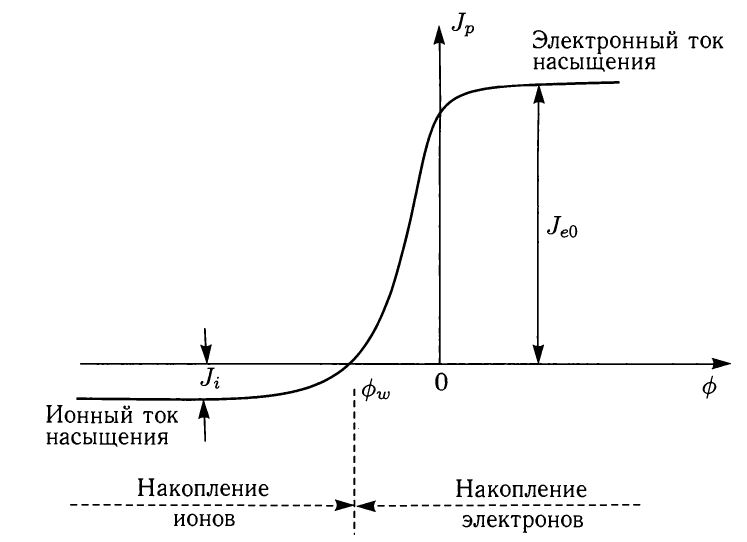
\includegraphics[width=70mm]{VaH_zonda.JPG}
	\end{center}
\end{figure}
электронов 
Характерная вольтамперная характеристика электростатического зонда, помещенного в плазму. Плавающий потенциал зонда по отношению к потенциалу плазмы обозначен как $\phi_w$.
Зонд будет окружён так называемым плазменным слоем - в нём часть электронов прилетела на зонд, однако такое возмущение по размеру сравнимо с радиусом Дебая. 

В условиях равновесия число электронов, достигающих зонда в единицу времени, равно числу ионов, сталкивающихся с зондом в единицу времени. Предположим, что ток положителен, если 
он течет от зонда. Ток, связанный с электронами, направлен от зонда и, следовательно, рассматривается как положительный; электрический ток, создаваемый ионами, будет отрицательным. В условиях равновесия полный ток через зонд равен нулю и его потенциал равен плавающему потенциалу $\phi_w$.

Левая часть картинки.

Когда потенциал зонда делают меньше $\phi_w$ ток, 
создаваемый электронами, уменьшается, поскольку сила,  
отталкивающая электроны вследствие наличия у зонда электрического поля, возрастает. Если потенциал уменьшить еще сильнее, то ток, создаваемый электронами, станет пренебрежимо мал и полный электрический ток асимптотически приблизится к постоянному отрицательному значению, соответствующему плотности электрического тока J, связанной только с потоком ионов. 

Правая часть картинки.
С другой стороны, когда значение потенциала увеличивается с некоторого отрицательного значения $\phi_w$, количество электронов, достигающих зонда в единицу времени, становится больше количества ионов, поскольку сила, отталкивающая электроны, уменьшается и полный электрический ток становится положительным. Если электрический потенциал равен нулю, т. е. 
потенциал зонда становится равным потенциалу плазмы, то, поскольку тепловая скорость электронов существенно выше тепловой скорости ионов, плотность электрического тока $J_{0e}$ становится намного больше плотности тока, создаваемого ионами. Если потенциал становится положительным, то возникает ситуация, когда током, создаваемым ионами, можно пренебречь, но все электроны, достигающие границы слоя, попадают на зонд. Для достаточно больших положительных значений $\phi_w$ плотность электронного тока становится постоянной. Область плато на вольтамперной характеристике зонда называется областью насыщения электронного тока.
Если начать ещё больше увеличивать потенциал зонда, то ток из насыщения будет ещё расти, это потому, что большой потенциал вносит большое возмущение в область вокруг себя и ток растёт из-за роста этой области (с которой собирают электроны)

Ток на зонд в отсутствии поля:
\begin{equation}
	J_{0e}=e n_e (\frac{kT_e}{2 \pi m_e})^{1/2}
\end{equation}
При увеличении потенциала, электронная компонента тока будет:
\begin{equation}
	J_{e}=J_{0e}exp(\frac{e\phi}{kT_e})
\end{equation}
Если рассмотрим отрицательный $\phi_w$, то ток ионный будет на зонд:
\begin{equation}
	J_{p}=J_{0e}exp(\frac{e\phi}{kT_e})-J_i
\end{equation}
Можно выразить из уравнений температуру:
\begin{equation}
	T_e= \frac{e}{k} (\frac{d}{d \phi} [ln(J_p + J_i)])^{-1}
\end{equation}
То есть, мы сняли ВАХ плазмы, построили её в логарифмическом масштабе, тогда НАКЛОН такой ВАХ и будет температурой электронов.
Концентрацию плазмы мы тоже можем вычислить, подставив известную температуру:
\begin{equation}
	n_e= \frac{J_{e0}}{e} (\frac{2 \pi m_e}{kT_e})^{1/2}
\end{equation}


Но это одиночный зонд. Зачастую делают двойной зонд. Это 2 проволочки, которые расположены рядом друг с другом, на одну подаём + потенциал, на другую - и замеряем ток между ними. Зачем это нужно?

При таком расположении, у нас ОБА электрода находятся внутри плазмы, а как следствие в одинаковом потенциале плазмы (при $\phi_w=0$ у нас 0 тока). так же, электроны оч лёгкие и так получается, что все электроны, которые ушли с одного электрода, пришли на второй. Тем самым, исключаем ток электронов. По факту, двойной зонд снимает только ионный ток + получаем симметручную ВАХ.
\begin{figure}[ht]
	\begin{center}
		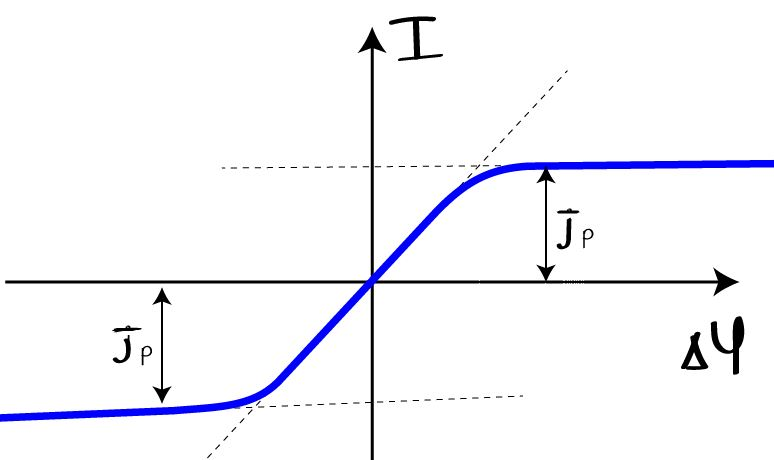
\includegraphics[width=70mm]{VaH_zonda_2.JPG}
	\end{center}
\end{figure}
Аналогичным с электронами образом, можно вывести температуру ионов как:
\begin{equation}
	T_i= \frac{J_p}{2 \frac{d I}{d \phi} |_{\phi=0}}
\end{equation}

Применимость зондов - зонды маленькие, плазма бесстолкновительная.

Метод магнитных зондов.
Используются в термоядерных реакторах при не слишком малых $\beta=p8\pi/B^2$. Магнитная катушечка, ориентированная нужным образом, помещается в точку где надо исследовать параметры среды. Обычно это катушечка около 1 мм в фарфоровой трубке. Располагая её в различных точках, получаем данные о магнитных линиях через наведённый ток.

Температуру в точке находим как:
\begin{equation}
	n k(T_e + T_i)= \frac{B_{\text{ext}}^2}{8 \pi} - \frac{B_{\text{int}}^2}{8 \pi}
\end{equation}
, где $B_{ext}$ и $B_{int}$ - внешнее и внутреннее магнитное поле.
 

\subsection{Оптические методы}

Определение электронной температуры по интенсивности излучения линейчатого спектра.

При релаксации возбуждённого состояния между уровнями испускается квант с частотой $\nu=\frac{E_2-E_1}{h}$ и интенсивность излучения из объёма будет равна $I=h\nu n_{2} A_{21}$, где $A_{21}$ - вероятность перехода (коэф. Эйнштейна).
\begin{equation}
	n_1 u(v)B_{12}+n_e n_1 \langle\sigma_1 v\rangle=n_e n_2 (\sigma_2 v) + n_2 A_{21}+n_2 u(v) B_{21}
\end{equation}

, где $n_1$ - концентрация атомов в состоянии 1, $n_2$ - концентрация атомов в сост. 2, $n_e$ - концентрация электронов, $v$ - скорость электронов, $\sigma_1$ эффективное сечение возбуждения, $\sigma_2$ - эффективное сечение, снимающее возбуждение, $u(v)$ спектральная плотность излучения в плазме, $B_{12}, B_{21}$ - коэффициенты эйнштейна. В опытах обычно смотрят на излучение оптически прозрачной плазмы (ничего не поглощает) Есть 2 предельных случая.

\subsubsection{Плазма низкой концентрации}

Считаем так, если происходит мгновенное высвечивание (пренебрегаем снятие возбуждение ударами)
Уравнение выписывается упрощается до 
\begin{equation}
	n_e n_1 \langle\sigma_1 v\rangle= n_k  \sum\limits_{i=1}^{k-1}A_{k i}
\end{equation}
$A_{k i}$ коэффициент эйнштейна для релаксации с уровня k на уровень i.
Следовательно интенсивность излучения 
\begin{equation}
	I=h \nu n_k A_{k1}=h \nu n_e n_1 \langle\sigma_1 v\rangle\frac{A_{k1}}{\sum\limits_{i=1}^{k-1} A_{ki}}
\end{equation}

Для резонансной линии отношение $A/\sum A $ равно единице. так же, если мы знаем $n_e, n_i$ и зависимость $\langle\sigma_1 v\rangle$ от температуры, то можем определить температуру плазмы по отношению относительных интенсивностей двух линий.

\begin{equation}
	\frac{I_1}{I_2}= \frac {\nu_1 \langle\sigma_1 v\rangle_1 A_1 \sum A_k^{(2)} }{\nu_2 \langle\sigma_2 v\rangle_2 A_2 \sum A_k^{(1)} }
\end{equation}
Это самое общее выражение. Далее, можно делать различные предположения (наверное уже не нужно). например, аппроксимировать сечение возбуждения функциями (стр. 45-46).
Не обязательно даже смотреть сваливание на основной уровень.

\subsubsection{Плазма высокой концентрации.}

Это такая концентрация, что $n_e \langle\sigma_2 v\rangle \gg A$ 
При выполнения этого условия в отсутствие фотовозбуждения устанавливается между детально обратными процессами $n_1 \langle\sigma_1 v\rangle = n_2 \langle\sigma_2 v\rangle$.
Используя известное выражение, для отношений вероятности прямого и обратного процессов:
\begin{equation}
	\frac{\langle\sigma_1 v\rangle}{\langle\sigma_2 v\rangle} = \frac{g_1}{g_2} e^{-\frac{E}{kT_e}}
\end{equation}
, где $E$ -  энергия уровня, $g_2$ и $g_1$  - статистические веса соответственно основного и возбуждённого состояний.
В этом случае значение интенсивности спектральной линии, отвечающий переходу из состояния с энергией возбуждения E в основное состояние равно:

\begin{equation}
	I=\frac{h \nu n_1 A g_2}{g_1} e^{-\frac{E}{kT_e}}
\end{equation}
Собственно, отношение двух линий для плазмы высокой концентрации, не зависит от концентрации, а зависит от температуру.
\begin{equation}
	\frac{I_1}{I_2}=\frac{ \nu_1 A_1 g_1}{ \nu_2 A_2 g_2} e^{-\frac{E_1 - E_2}{kT}}
\end{equation}

Т.е. если в эксперименте с электронами распределёнными по больцману измерить интенсивности линий, то можно вывести значение температуры плазмы. 

\subsubsection{определение параметров плазмы по форме спектральных линий}

Контуры спектральных линий атомов деформируются под действием внешних факторов.
\subsubsection{Определение ионной температуры по доплеровскому уширению спектральных линий}



Из-за допплера длина волны смещается на 
\begin{equation}
	\Delta \lambda = \lambda_0 \left(1+\frac{v_x}{c}\right)
\end{equation}
Если распределение максвеловское, то  значение составляющей $v_x$  в пределах от  $v_x$  до $v_x + dv_x$ определяется формулой:
\begin{equation}
	\frac{dn}{n}=\left(\frac{M}{2\pi kT_i}\right)^{1/2} e^{-\frac{Mv^{2}_x}{kT_i}} dv_x
\end{equation}

Из двух этих формул можно получить распределение спектральной плоскости.
\begin{equation}
	I=I_0 e^{-\frac{Mc^{2}}{2kT_i} (\frac{\Delta \lambda}{\lambda_0})^{2}}
\end{equation}

Обычно, определяют полуширину линии. Полуширина линии с температурой связана с температурой.
\begin{equation}
	\delta \lambda_D=\frac{2 \sqrt{2k \ln{2}}}{c} \lambda_0 \sqrt{\frac{T_i}{M}}
\end{equation}


\begin{equation}
	T_i(eV)=1.7*10^{8}A\left(\frac{\delta \lambda_D}{\lambda_0}\right)^{2}
\end{equation}
, где $A$- атомный вес иона.

\subsubsection{эффект доплера на рассеянном свете. Определение электронной температуры.}

Рассмотрим рассеяние монохроматического луча в плазме (оптически тонкой). Если длина волны падающего света много меньше среднего расстояния между заряженными частицами плазмы, а так же меньше дебаевского радиуса, то эффект взаимодействия излучения с плазмой определяется рассеянием на электроне формулой Томпсона: $\sigma =\frac{8\pi}{3} (\frac{e^{2}}{mc^{2}})^{2}$ и для электронов составляет $6.65*10^{-25} cm$.
При работе с плоскополяризованным светом рассеяние не является изотропным и мощность излучения под углом $\theta$ к направлению электрического вектора первичного излучения:

\begin{equation}
	W_{s} (\theta) d\theta=\left(\frac{e^{2}}{mc^{2}}\right)^{2} W_0 \int_{0}^{L} n \dd l \cos^{2}\theta \dd \theta
\end{equation}
, где n -  концентрация, а L - путь пучка в плазме.

При максвелловском распределении электронов по скоростям полуширина линии рассеяного света выражается следующим образом.

\begin{equation}
	\delta \lambda_s = 3.3*10^{-3} \lambda \sqrt{T_e (eV)}
\end{equation}
Это можно сделать в предположении не очень большой концентрации, когда лина волны лазера не слишком велика по сравнению с радиусом дебая.
\begin{equation}
	\alpha = \frac{\lambda}{4\pi \sin(\frac{\theta}{2} \lambda_D)} \ll 1
\end{equation}

, где $\theta$ - угол рассеяния, $\lambda_D$ - дебаевский радиус

Это подробно рассмотрено в работе Розенблюта и Ростокера и можно получить окончательное значение для интенсивности света:
\begin{equation}
	I=I_0 \exp{- \frac{1}{2} (\frac{\Delta \lambda}{\lambda} \frac{c}{\sqrt{kT_e /m}})^{2}}
\end{equation}


\subsubsection{ Штарковское уширение спектральных линий в плазме. определение концентрации ионов.}

В плазме на размерах порядка радиуса дебая, в плазме присутствуют микрополя. Микрополя есть электронные и ионные. Электронные быстро осциллируют, а вот ионные - нет, которые в $\sqrt{M/m}$ раз меньше электронных. Скорости ионов в $\sqrt{m/M}$ раз меньше, то можно полагать, что неподвижный атом находится под быстрым воздействием электронов, находясь в слабоменяющимся поле иона. 

И энергитические уровни возбуждённого атома, находясь под действием этого внешнего электрического поля, расщепляются. А за счёт быстродействующих микрополей электронов, осуществляется переход между штарковскими подуровнями или в результате резкого изменения величины и направления поля происходит сильное изменение фазы излучаемой световой волны. 

Вызванное электронами уширение ОТДЕЛЬНОЙ штарковской компоненты спектральной линии может быть описанной с помощью ударной теории.
\begin{equation}
	I_s=\frac{\gamma}{(\omega + \omega_0 - d)^{2}+ \frac{\gamma^{2}}{4}}
\end{equation}
, где $\omega_0$ - частота линии, $d$ -  смещение линии в электрическом поле
По сути, полуширина линии - обратное время время жизни атома в данном возбуждённом состоянии $\gamma =n_e \langle\sigma v_e\rangle$.
Сечение электронных столкновений можно записать как $\sigma \sim \pi \rho^{2}$

В квазиклассическом приближении переход из одного возбуждённого состояния в другое под действием столкновений возможен в том случае, есди время пролёта частицы становится сравним с временем перехода между состояниями. В водородном приближении это:
\begin{equation}
	\frac{v}{\rho}=\frac{\left\langle d_{m m'}\right\rangle  e}{\hbar \rho^2}
\end{equation}
Здесь $\left\langle d_{m m'}\right\rangle $ - дипольный момент перехода штарковскими коспонентами. записывая его в виде $k^2 a_{0} e$.
Подставляя значение радиуса боровской орбиты приводит, к $\rho \sim \frac{k^2 \hbar}{Zmv}$. Поэтому подставляя это в формулу для сечения получаем, что:
\begin{equation}
	\sigma = \pi k^4 \left(\frac{h}{mv}\right)^2 Z^2
\end{equation}

В действительности из-за дальнодействуюшего характера дипольного взаимодействия в правую часть этого выражения необходимо добавить множитель $L= \ln(\frac{m v_e^{2}}{E-E_1})$ , котрый можно заменить 10.

Критерий применимости ударной теории - длительность столкновений много меньше времени между столкновениями, т.е. $\frac{n^{-1/3}}{v_e} \ll \frac{1}{n \langle\sigma v_e\rangle} $ выполняется тем лучше, чем выше концентрация плазмы и чем выше температура.

Так же, данная теория хорошо описывает только хорошо отстоящие от центральной линии (при штарковском уширении происходит разложение несущей спектральной линии)

Для центральной линии это не выполняется (оч маленькие расстояния между подуровнями штарковскими $\omega - \omega_0 \leq \gamma$).
Тут вступает в силу теория, которая затрагивает микрополя в плазме, а именно, Хольмарк выдвинул теорию о распределении микрополей в плазме, а именно вероятность поля:
\begin{equation}
	H( \beta ) = \frac{2}{\pi \beta} \int_{0}^{\inf} v \sin(v e^{- (\frac{v}{\beta})^{3/2}}) dv
\end{equation}
, где $\beta = \frac{E}{E_0}$ , $E_0 = 2,61 e n^{2/3}$ 
Физический смысл $E_0$ прост: Среднее расположение между частицами плазмы $\frac{1}{n^{1/3}} $, а напряжённость поля точечного заряда обратно пропорциональна квадрату расстояния. Форма функции Хольцмарка:
\begin{figure}[ht]
	\begin{center}
		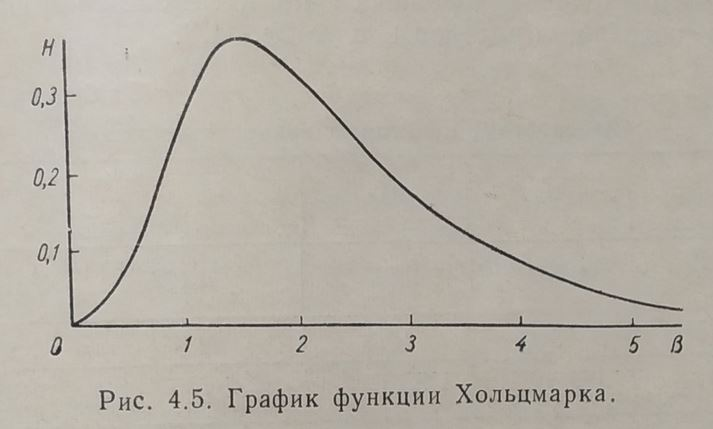
\includegraphics[width=85mm]{Holsmark.JPG}
	\end{center}
\end{figure}

В этом случае контур линии центральной в рамках применимости запишется как 
\begin{equation}
	I_{st}=\frac{1}{\Delta \omega_0} H(\frac{\omega-\omega_0}{\Delta \omega})
\end{equation}
В этой формуле в случае линейного эффекта Штарка: $\Delta \omega_0 = 2.61 \alpha n^{2/3}$

\subsubsection{Сплошной спектр. определение концентрации и электронной температуры}

Форма и интенсивность непрерывного спектра излучения плазмы определяется протеканием следующих процессов:
1.Тормозное излучение при взаимодействии электронов с ионами
2.Рекомбинационное излучение, возникающее при радиационном захвате электрона ионом.
3.Тормозное излучение, возникающее в результате электрон-электронных взаимодействий.

Из всех трёх остановимся на первых двух, ибо 3 играет роль в релятивистской плазме и обычно её не наблюдают.

Посмотрим на интенсивность рекомбинационных линий.
\begin{equation}
	I_{rec} \dd\nu = A n_i n_e (\frac{E_H}{kT_e})^{3/2} (\frac{E_{ik}}{E_H})^{2} \frac{g_{fb}}{k} \xi_k e^{\frac{(E_{ik}-h \nu)}{kT_e}} \dd\nu 
\end{equation}
Здесь $E_H = 13.6 eV$ энергия ионизации водорода. $E_{ik}$ - энергия ионизации оболочки, для которой главное квантовое число равно $k$, $g_{fb}$ - множитель Гаунта для свободно-связанных переходов.$ \xi_k$ - число квантовых мест на $k$-ой оболочке (если пустая, то $ \xi_k = 2k^{2}$ ). 
Видно, что мощность рекомбинационного излучения пропорциональна $Z^{4}/k^3$
Видно, что этот спектр имеет РЕЗКУЮ границу. Нету фотонов с энергией меньше чем $E_{ik}$, а с другой стороны есть длинный хвост, который описывается степенью экспоненты делённую на температуру. По этому хвосту и можно восстановить температуру

\begin{figure}[ht]
	\begin{center}
		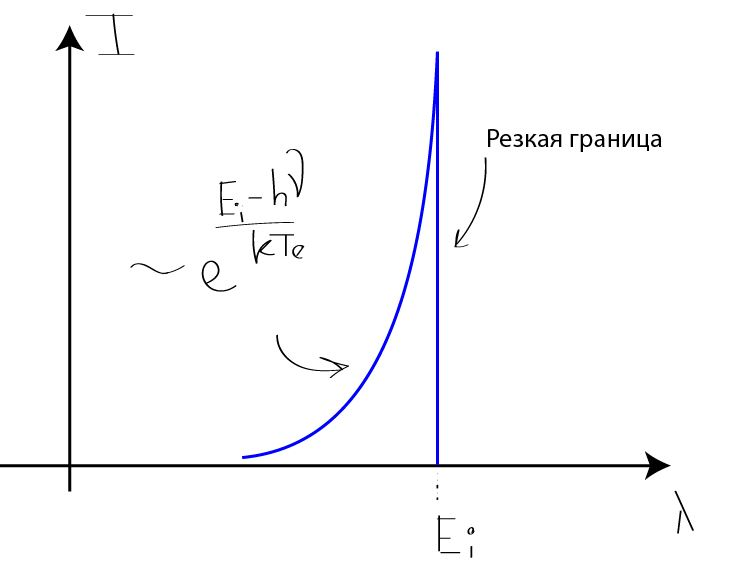
\includegraphics[width=70mm]{Intencity_recomb.JPG}
	\end{center}
\end{figure}

В случае тормозного излучения, обусловленного свободно-свободными переходами, в отличие от рекомбинационного, неограниченно простирается в сторону длинных волн. Мощность излучения в единице объёма плазмы в телесном угле $4 \pi$ , приходящийся в интервал частоты $d\nu$.

\begin{equation}
	I_{torm} \dd\nu = A Z^{2} n_i n_e (\frac{E_H}{kT_e})^{1/2} e^{-\frac{h \nu}{kT_e}} g_{ff} \dd\nu
\end{equation}
, где $g_{ff}$ множитель граута, который в широком диапазоне температур имеет сложный характер, но он порядка 1.

В общем, если смотреть на мощность излучения, то она для тормозного излучения будет:
\begin{equation}
	Q_{torm}=1.5 *10^{-25} Z^{2} n_e n_i T^{1/2}[eV]
\end{equation}
\begin{equation}
	Q_{rec}=5 *10^{-24} Z^{4} n_e n_i T^{-1/2}[eV]
\end{equation}

Видно, что для водородоподобной плазмы, они сравниваются для энергий 30eV. Свыше 100ev основной вклад в континуум даёт тормозное излучение.

\subsubsection{Сплошной спектр. ИК область}

Он интересен тем, что измерения проводятся в большом диапазоне энергий. Можно мерить и концентрацию и эл. температуру.
Необходимо выбрать такой участок спектра, внутри которого происходит переход от объёмного тормозного спектра излучения к поверхностному.
Поверхностное излучение отвечает случаю отвечает излучению чёрного тела и реализуется для слабого поглощения в плазме. Мощность излучения чёрного тела зависит только от температуры, то есть измерив его мощность - определим температуру.

По скольку в широкой области концентраций и электронных температур самопоглощение ИК излучение можно не учитывать, концентрация плазмы связана с температурой электронов формулой:
\begin{equation}
	n=3.9*10^{19} T_e^{\frac{1}{4}}[eV] (\frac{\int_{\Delta \nu g_{ff}} I(\nu) d\nu}{\Delta \nu g_{ff}})^{\frac{1}{2}}   cm^{-3}
\end{equation}

\subsubsection{Определение диэлектрической проницаемости плазмы. СВЧ метод}

Вспоминаем, что распространение ЭМ волн в плазме определяется диэлектрической проницаемостью.
\begin{equation}
	\epsilon = 1- \frac{\omega_{pl}^{2}}{\omega^{2}} \frac{1}{1-i \frac{\nu_{collision}}{\omega}}
\end{equation} 
, где $\nu_{collision}=\frac{2*10^{-5} n_i Z}{T_e^{3/2}[eV]}$, $\omega$ - частота волны

В случае малого поглощения, убирается мнимая часть.
\begin{equation}
	\epsilon = 1- \frac{\omega_{pl}^{2}}{\omega^{2}} 
\end{equation} 
Тоесть, если мы сможем измерить эпсилон для среды и конкретной частоты - узнаем и $\omega_pl = \sqrt{\frac{4 \pi e^{2} n_e}{m}}$, то узнаем концентрацию $n_e$

То есть что делают, берут какой-то СВЧ генератор, светят на плазму. Если проходит, значит концентрация меньше критической для данной частоты. Если отражается назад, то значит внутри есть слой с критической концентрацией. Это метод отсечки.
Оправданно это при условии $l \gg \frac{c}{\omega_pl}$
, где $l$ - толщина слоя плазмы с концентрацией выше критической, $\omega_pl$ - плазменная частота.

Если такой слой достаточно мал, то прибегают к интерферометрии. Собирают установку, где часть СВЧ сигнала проходит по участку, занятому плазмой, половина по свободному тракту. Далее, сигналы суммируют в интерферометре. По амплитуде суммарного сигнала, можно судить о разности фаз.

\begin{figure}[ht]
	\begin{center}
		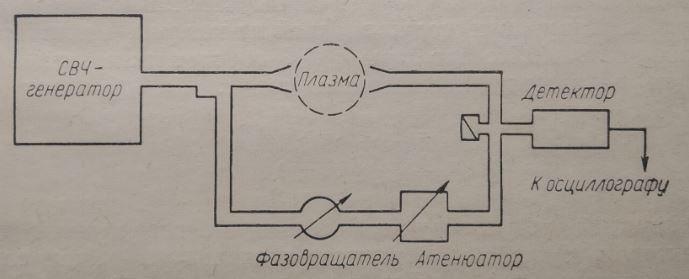
\includegraphics[width=70mm]{HF interferometre.JPG}
	\end{center}
\end{figure}

 Очевидно, что разность фаз - набег фазы по пути через плазму с коэффициентом преломления N.
 \begin{equation}
 	\phi = \frac{2 \pi}{\lambda} \int_{0}^{l} [N_0 - N(x)] dx 
 \end{equation} 
, здесь $l$ - размер плазмы, $N=\sqrt{\epsilon}$ - показатель преломления, $\lambda$ - длина волны СВЧ. Вообще, если тракт откачан воздухом, то $N_0 =1$


\subsubsection{Определение диэлектрической проницаемости плазмы. Применение лазеров}

Когда частоты СВЧ не хватает, для большой концентрации плазмы, используют лазеры.
Принцип абсолютно тот же, лазерный пучок пропускают через плазму и интерферируют самим с собой. На экране камеры получают интерфериционную картинку в виде полос. Потом, когда на пути пучка возникает плазма, в тех местах где увеличена концентрация, там уменьшается показатель преломления среды и как следствие, интерференционная картина превращается в кривые полосы. По кривизне полос в каждой точке, можно судить о набеге фаз.

\subsubsection{Корпускулярные методы диагностики плазмы}

\subsubsection{Использование пучков заряженных частиц}

С помощью пучка можно исследовать оч быстрые изменения плазмы. Конфигурации эксперимента оч разные, поэтому приводятся лишь некоторые из них.
Первое это зондирование пучком плазмы для определения радиальной и азимутальной компоненты поля в магнитной ловушке. Двигаясь продольно магнитному полю, при наличии поперечного поля электроны будут испытывать дрейф в скрещенных полях. Помещая электронную пушку в области одной пробки, люминисцентный экран в другой пробке, можем вижеть отклонение эл пучка на экране.
В отсутствие плазмы пучок двигается вдоль линий магнитного поля и делает точку на люминофоре. Наличие дрейфового движения приводит к смещение на экране на расстояние
\begin{equation}
	\Delta x=\frac{cE_y}{H_z} * \frac{l}{v}
\end{equation}
. где $l$ - длина пути пучка в плазме, $E_y$ - составляющая электрического поля, перпендикулярная магнитному полю, $v$ - скорость движения электронов вдоль линий поля.
Соответственно, смещение по радиусу пучка это азимутальная компонента поля, смещение по углу - радиальная компонента поля E.

Для определения потенциала плазмы относительно стенок используют метод, основанный на запирании пучка электронов. Время пролёта через плазму:
\begin{equation}
	\tau = \sqrt{\frac{M_i}{2Z_i}} \int_{0}^{l} \frac{dx}{\sqrt{V_0 +V(x)}}
\end{equation}
, где $Z_i$ - заряд иона.$M_i$ - масса иона, $l$ - размер плазмы, $V_0$ ускоряющий потенциал в источнике ионов, $V(x)$ - распределение потенциала вдоль пути пучка.
Если падение потенциала почти всё сосредоточено в дебаевском рабиусе, значительно меньшим $l$, то выражение будет
\begin{equation}
	\tau = \frac{l}{v_i}
\end{equation}
, где 
\begin{equation}
   v_i= \sqrt{\frac{Z_l (V_0 + V_pl)}{M_i}}
\end{equation}

Область применимости- не должны влиять неустойчивости. Время прохождения через плазму должно быть меньше, чем время развития неустойчивостей.
\begin{equation}
	\tau_{neust} =(\frac{n}{n'})^{1/3} \frac{1}{\omega_{pl}}
\end{equation}
, где $n'$ - концентрация электронов в пучке.




\subsubsection{Измерение концентрации нейтральных и заряженных частиц.}

Прохождение пучка атомов или ионов через плазму сопровождается атомными и электронными столкновениями, приводящие к изменению заряда пучка. И то, на сколько он потеряет заряд - тоже будет функция температуры и концентрации электронов.
Рассмотрим изменение зарядового состояния монохроматического атомного пучка, состоящих из нейтральных атомов и протонов водорода, при прохождении через водородную плазму.
Средне квадратичный угол отклонения пучка будет:
\begin{equation}
 \overline{\theta} = 2 (\frac{Z_1 Z_2 e^{2}}{M v^2}) \sqrt{2 \pi nLl}
\end{equation}
, где $l$ - длина пути пучка в плазме с концентрацией $n$, $L$ - кулоновский логарифм ($L \sim 15$); $M$ - масса частицы пучка.
Для водорода с энергией электрона $10^{4} eV$ для $nl \sim 3*10^{16}$ среднеквадратичный угол будет $1.5^{\circ}$ 
Основные элементарные процессы плазмы с пучком.
1. Захват быстрым протоном электрона при взаимодействием с нейтральными атомами плазмы.
2. Обдирка электрона, принадлежащему быстрому атому, при взаимодействии его с нейтральными атомами среды.
3. Обдирка электрона, принадлежащему быстрому атому на протонахх плазмы.
4. Ионизация быстрых атомов электронами плазмы. 
Для описания каждого процесса, по факту пишут баланское уравнение по трассе пучка:
\begin{equation}
	\frac{dN_0}{dl} = -N_0 n_0 \sigma_{01}-N_0 n_i \sigma_{10} 
\end{equation}
и т.п., решаем с граничными условиями, сравниваем с экспериментом, делаем предположения о температуре плазмы и концентрации. Непосредственно сам пучок измеряется с помощью масс-спектрометров.


\subsubsection{Масс-спектроскопическая методика исследования быстрых частиц плазмы}

 Пучок, выходящий из плазмы, направляется в магнитное поле. В зависимости от массы и заряда, все частицы отклоняются на разные углы. Приближённо, отклонение на экране регистратора можно записать как
 
 \begin{equation}
 	x=\frac{ZeHl^{*}h}{Mv}
 \end{equation}
, где $l^{*}$ - расстояние между магнитом и детектором, $h$- протяжённость магнитного поля

\subsubsection{Калометрические измерение плазмы}

Есть несколько измерений.
1. Определение кривой распределения потоков тепла на стенку в относительных единицах.
2. определение энергии на данный участок поверхности.
3. Определение временного хода тепла.


Проще всего 1-я задача. Если на единице поверхности теплообменника выделяется количество тепла в Q калорий, то увеличесние его температуры определяется формулой.
 \begin{equation}
	\Delta \theta= \frac{Q}{dch} (1-\gamma)
\end{equation}
Здесь $d$ - плотность, $c$ - теплоёмкость и $h$ - толщина теплоприёмника, а $\gamma$ коэффициент отражения плазмы (обычно равен десятку процентов)
Вообще для измерения используют балометры. Так же можно исследовать мощность в зависимости от времени.
 \begin{equation}
	\Delta \theta= \int_{0}^{t} \frac{1}{dch} \frac{dQ}{dt}
\end{equation}

\subsubsection{Регистрация жёстких излучений плазмы}

Используют метод наведённой радиоактивности для того, чтобы обнаружить и измерить нейтронные импульсы интенсивности $10^4 - 10^5$ нейтронов и выше.
В естественном серебре есть два изотопа. $Ag^{107} Ag^{109}$ примерно в равных количествах. Сечения захвата 44 и 110 Барн соответственно. В следствие захвата образуются  $Ag^{108} Ag^{110}$ с периодом полураспада 2,4мин и 24,5сек, которые испытывают $\beta$ распад, который можно регистрировать. Собственно минимальная длительность определяется именно минимальным полураспадом, скважность между ними - максимальным временем полураспада.
Следующий метод - сцинтиляторный регистратор. ЧТо это такое. Ставят условный "друшлаг" - экран с большим количеством дырочек, за которым есть флуорисцирующий экран. Пучок нейтронов пролетает в дырки на друшлаге и попадают на экран, но из-за разлёта по углу, расстояние между светящимися точками на экране не такое как на друшлаге.

\begin{figure}[ht]
	\begin{center}
		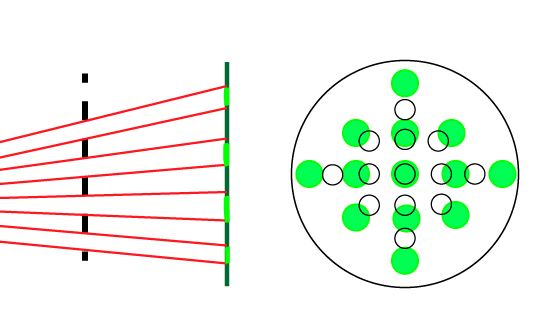
\includegraphics[width=70mm]{scintelator.JPG}
	\end{center}
\end{figure}

Так же используют Камеру обскура и Камеру Вильсона.

\section{Электрический разряд в газах}

\subsection{Основные виды разряда: тлеющий разряд, искра, электрическая дуга, ВЧ-, СВЧ-и оптический разряд}
\subsubsection{Тлеющий разряд}
Характеризуется не очень большим током, малыми давлениями.
Быстрее всего описан: [Сивухин, общий курс физики, 3 том., параграф 117]

\begin{figure}[ht]
	\begin{center}
		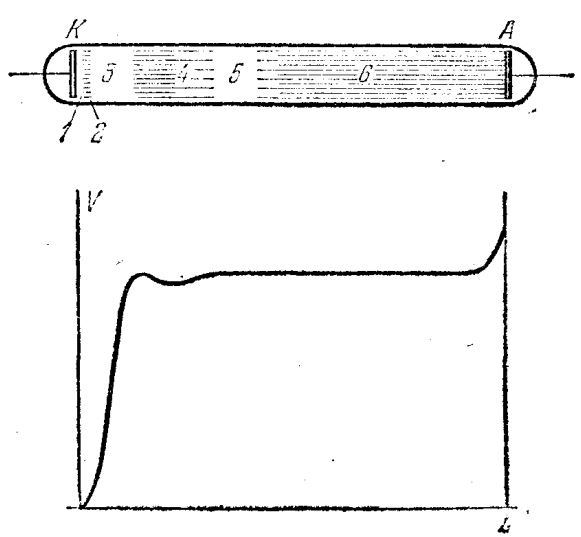
\includegraphics[width=70mm]{12.1.JPG}
	\end{center}
\end{figure}

Область 1 - область эмиссии электронов. 2 - катодный слой, идёт возбуждение нейтралов электронами, 3 - тёмное катодное пространство, область где происходит первичная ионизация, тут происходит затравка электронной лавины 4 - область рекомбинации ионов, идущих справа, и электронов, идущих слева. 5 - тёмное андоное пространство - ионов не так много, электроны ещё не успели снова набрать скорость. Все предыдущие области отвечали за поддержание лавины. Именно они определяют её существование  6 - положительный андоный столб/анодное свечение, в основном вызванное рекомбинацией электронов с ионами, которые были образованы на расстоянии нескольких пробегов до анода. Область эта характеризуется высоким зарядовым числом ионов, высокой проводимостью.
\subsubsection{искровой разряд}
[Сивухин, общий курс физики, 3 том., параграф 118]

Характеризуется большими давлениями и большим напряжением пробоя.
Имеет ломанную форму, так как в следствие первичного пробоя стримером, возникает канал ионизации, по которому начинает течь ток огромный ток, который вслед за собой вызывает возбуждение и свечение в УФ диапазоне. Вблизи канала УФ излучением ионизуются новые молекулы, которые становятся затравками для новых искр. Поэтому, форма очень ветвистая.

\subsubsection{коронный разряд}
[Сивухин, общий курс физики, 3 том., параграф 119]
Возникает при больших давлениях в сильно неоднородных полях (острия игл). В зависимости от напряжения на игле может быть 2 разных разряда. С положительной короной и отрицательной.
У отрицательной короны положительные ионы образуются электронными лавинами, которые были ускорены в области неоднородного поля катода. Ионы попавшие на катод, выбивают ещё электронов.
В случае положительной короны,  электронные лавины пораждаются фотоионизацией самой же короны.

\subsubsection{дуговой разряд}
[Сивухин, общий курс физики, 3 том., параграф 120]
Характеризуется большим током, малым напряжением, большими давлениями.
После первичного пробоя газа, по каналу начинает бежать большой ток. Сопротивление канала резко падает. Из-за большого тока, электроны с собой захватывают и часть электродов. тем самым, лавина поддерживается термоэмиссией заряженых частиц с электродов.

\subsubsection{ВЧ разряд}
[райзер Ю.П., лазерная искра и распространение разрядов, гл 7, пар 28]
До этого всё были пробои в относительно стационарных полях, но для разряда это вовсе не обязательно. Большая напряжённость эл поля может быть достигнута и другими способами. Например, собирается колебательный контур с большими конденсаторами и катушкой. Конденсаторы сначала заряжаются, а потом замыкаются через катушку (индуктор). В катушке подскакивает ток, как следствие внутри возникает большое магнитное поле, которое порождает электрическое, которое в свою очередь вызывает разряд.

\begin{figure}[ht]
	\begin{center}
		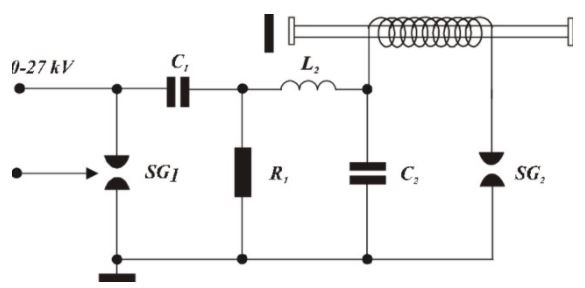
\includegraphics[width=70mm]{12.5.jpg}
	\end{center}
\end{figure}

на рисунке приведена схема лазера, активная область которого создаётся индукторным разрядом.
В том случае, если у нас не импульсно будет происходить разрядка конденсаторов, а мы будем поддерживать колебания в этом контуре, то это будет ВЧ разряд индукционного типа.
[райзер, физика газового разряда, 3-е изд, глава 18.2]
Так же есть ВЧ разряд ёмкостного типа. Внутри конденсатора создаётся область переменного электрического поля. Которую можно рассматривать как конденсатор с проводимостью. И из-за этого ток может быть смещён по фазе, относительно внешнего напряжения, что ограничивает мощность.
\subsubsection{СВЧ разряд}
Переменное в пространстве поле можно создавать вообще без электродов, например СВЧ пучком. Так как энергия кванта СВЧ излучения мала, то ясно что “нагрев” (набор энергии электронов) происходит на столкновениях,  так как если бы вообще не было столкновений, то электрон бы энергию в переменном поле не набирал. Понятно, что чем больше поле, тем быстрее электрон в нём набирает энергию, однако у нас появляется поправка, связанная с частотой соударений, а именно если вспомнить “нагрев на столкновениях” то там можно ввести эффективное поле греющее поле $E_{eff}=E \frac{\nu_{tr}^{2}}{\nu_{tr}^{2}+\omega^{2}}$. 
\subsubsection{Лазерный разряд / лазерная искра}
[райзер Ю.П., лазерная искра и распространение разрядов, гл 1, пар 1]
Тут основным механизмом создания плазмы разряда естественно тоже будет ионизация. Однако она может иметь двух видов. 1) нагрев на столкновениях (в достаточно большом поле, ИК область) 2) фотоионизация (многоквантовый процесс при большой интенсивности света и большой энергии кванта)

\subsection{Условия стационарности разряда, излучающий разряд в плотной плазме, плазменно-пучковый разряд}
\subsubsection{Условие стационарности разряда}

Вообще, условие стационарности ЛЮБОГО разряда,  это частота рождения электронов должна быть равна частоте их гибели. $\nu_{born} = \nu_{death}$ . Рождение электронов - инонизация любых видов, отлипание от отрицательного иона. Гибель - диффузия всех видов, рекомбинация, так же туда относят потери энергии на возбуждение частиц, хотя электроны непосредственно не теряются, но они теряют энергию. Тем самым, замедляется рост электронной лавины. 

\subsection{Излучение разряда в плотной плазме}

?
ну понятно, что в разряде будут возбуждаться молеулы, будет происходить рекомбинация. Понятно, что все эти линии будут видны. В случае равновесного разряда ($T_e = T_i$), у нас будет ещё и излучение чёрного тела.

\subsection{Плазменно-пучковый разряд}

Плазменно-пучковый разряд - один из видов электрич. разрядов в газе, при котором в межэлектродное пространство вводится ускоренный пучок электронов и плазма разряда разогревается гл. обр. за счёт пучковой неустойчивости. В результате развития неустойчивости ср. энергия электронов в пучке уменьшается, часть энергии пучка передаётся ленгмюровским волнам, которые затем передают её тепловым электронам плазмы. Разогрев тепловых электронов происходит за счёт затухания ленгмюровских волн при столкновениях, при их рассеянии на тепловых электронах с трансформацией ленгмюровских волн в ионнозвуковые и т. д.
Доля $\alpha$ энергии пучка, трансформируемая в энергию ленгмюровских волн, зависит от первоначального разброса скоростей электронов пуч­ка и от длины взаимодействия пучка с плазмой. Наибольшие значения $\alpha$  (порядка 1) реализуются для пучка, достаточно размытого по скоростям.
В П.п. р. значит. вклад в ионизацию вносят разогретые тепловые электроны плазмы, концентрация которых по мере развития разряда обычно начинает превышать концентрацию электронов в пучке. На формирование функции распределения тепловых электронов оказывают влияние упругие и неупругие столкновения, а так­же ускорение электронов в электрич. полях ленгмюровских колебаний.


\section{ Гидродинамические и тепловые явления в плазме}

\subsection{Ударные волны в плазме}

Как и в обычном газе, волны большой амплитуды могут распространяться в плазме со скоростью, большей скорости звука. По мере распространения таких волн они становятся круче и происходит образование \uline{ударных волн}, т. е. движущихся тонких слоев -- фронтов, разделяющих области с разной плотностью и температурой. В нейтральном газе скорость звука является универсальной величиной, процесс увеличения крутизны волн уравновешивается диффузией поперек фронта, а изменение состояния вещества при прохождении через фронт происходит благодаря парным столкновениям. В плазме же существуют различные ``звуковые'' волны, и плазменная ударная волна может образоваться на любой из них~\cite{kroll}.

Увеличение крутизны волн в плазме может быть уравновешено наряду с диффузией также и дисперсией волн: более короткие волны, необходимые для образования более узкого фронта, распространяются медленнее и отстают от ударной волны. Волны, в которых увеличение крутизны волн уравновешивается дисперсией, называются \uline{солитонами}, или уединенными волнами. Они распространяются в плазме наподобие локализованных возмущений конечной амплитуды. Состояние плазмы после прохождения через нее солитона может измениться вследствие парных столкновений, затухания Ландау, развития неустойчивостей или захвата и отражения частиц волной~\cite{kroll}.

Теперь рассмотрим ударную волну, летящую по ионизированному веществу~\cite{zeldovich}. Предположим сначала, что электронная теплопроводность не отличается от ионной. Кроме того, будем считать, что ионизация происходит не в самой ударной волне, а волна
распространяется по уже ионизованному газу. В системе координат, связанной с волной, значительная часть кинетической энергии газа, набегающего на \uline{скачок уплотнения} под действием сил ионной вязкости, необратимо переходит в тепло. Толщина вязкого скачка определяется временем между ионными столкновениями и порядка длины пробега ионов. Можно пренебречь передачей энергии от ионов к электронам, т.к. время теплопередачи порядка (где $\tau_{ei}$ -- время между столкновениями) $\tau_T=\sqrt{\frac{M}{m}}\tau_{ei}$ (см.~\ref{subsec:kinetic_eff_freq}). Электроны нагреваются, т.к. их утягивает за собой возникающее электрическое поле и происходит адиабатическое сжатие электронного газа~\cite{zeldovich}.

Например, для водорода показатель адиабаты будет $\gamma=5/3$ и температура электронов вырастет в $4^{\gamma-1}=2.5$ раз (температура ионов может расти выше). Потом за $\tau_{T}$ происходит релаксация температур. Характерное расстояние, на котором температуры электронов и ионов разные, можно оценить как $\Delta x \sim \frac{\rho_0}{\rho_1}D\tau_{T}$, где $D$ -- скорость фронта ударной волны (см. рис.~\ref{fig:shock_wave_T}).

Добавим в рассмотрение электронную теплопроводность, т.к. электроны быстрые. Коэффициент электронной температуропроводности равен:

\begin{equation*}
	\chi_e = \frac{l_e \overline{v_e}}{3} \approx \frac{\overline{v_e^{2}} \tau_e}{3},
\end{equation*}

где $l_e$ -- длина пробега электронов; $\overline{v_e}$ -- их тепловая скорость; $\tau_e$ -- время между столкновениями электронов друг с другом.

Как известно, длина пробега заряженных частиц зависит не от их массы, а только от заряда и температуры $l\sim\frac{T^{2}}{Z^{4}}$. Значит, для водородной плазмы ($Z=1$) длины пробега электронов и ионов одного порядка, однако, скорость электронов больше в $\sqrt{m_i/m_e}$ раз, чем ионов. Поэтому ионной теплопроводностью можно пренебречь. Характерный масштаб, на которой работает процесс электронной теплопроводности:

\begin{equation*}
	\lambda_e \sim \frac{\chi_e}{D} \sim \sqrt{\frac{m_i}{m_e}} \frac{\chi_i}{D} \sim \sqrt{\frac{m_i}{m_e}} l_i
\end{equation*}

Этот масштаб такого же порядка, что и ширина \uline{релаксационной зоны} выравнивания температур электронного и ионного газов:

\begin{equation*}
	\Delta x \sim D \tau_{ei} \sim D \sqrt{\frac{m_i}{m_e}} \tau_i \sim \frac{D}{\overline{v}} \sqrt{\frac{m_i}{m_e}} l_i \sim \sqrt{\frac{m_i}{m_e}} l_i
\end{equation*}

Поэтому по отношению к электронной теплопроводности градиенты в релаксационной зоне не малы и теплопроводностный теплообмен в этой зоне сравним с теплообменом между ионами и электронами. Электронная теплопроводность способствует скорейшему выравниванию температур за вязким скачком, так как она перекачивает тепло из более удаленных от скачка уплотнения слоев газа в передние, где электронная температура меньше. Рассмотрим теперь, насколько глубоко проникает тепло перед скачком уплотнения. Для этого запишем поток электронной теплопроводности:

\begin{equation*}
	S=-\kappa_e \dv{T_e}{x}=-\chi_e c_e \dv{T_e}{x},
\end{equation*}

где $\kappa_e = \upchi_e c_e$ -- коэффициент температуропроводности; $c_e$ -- теплоёмкость электронного газа при постоянном объёме. В силу стационарности процесса поток теплопроводности в прогревном слое равен гидродинамическому потоку электронной энергии [фактически -- ЗСЭ] (начальная температура электронов перед фронтом предполагается равной нулю; далеко перед волною поток $S$ исчезает):

\begin{equation*}
	-S= D c_e T_e = \upchi_e c_e \dv{T}{x}
\end{equation*}

Интегрируем выражение, зная, что $\chi_e=\alpha T_e^{5/2}$ ($a=const$), и получим, что:

\begin{equation*}
	x-x_0 = \frac{2}{5} \frac{a}{D} T_e^{-5/2} \Rightarrow T_e = \left[\frac{5}{2} \frac{D}{a} (x-x_0) \right]^{2/5},
\end{equation*}

где $x_0$ -- координата, где температура обращается в 0. Всё это изображено на рис.~\ref{fig:shock_wave_T_diff}.

\begin{figure}[ht]
	\begin{center}
		\begin{minipage}[ht]{0.49\linewidth}
			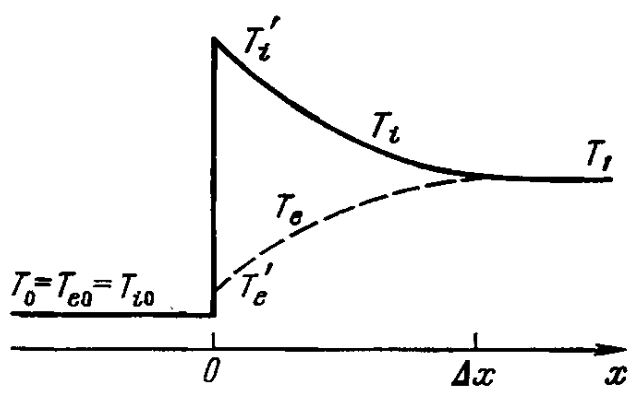
\includegraphics[height=0.15\textheight]{13. Skach plotn.JPG}
			\caption{Профили ионной и электронной (пунктир) температур во фронте ударной волны без учёта электронной теплопроводности~\cite{zeldovich}}
			\label{fig:shock_wave_T} 
		\end{minipage}
		\hfill
		\begin{minipage}[ht]{0.49\linewidth}
			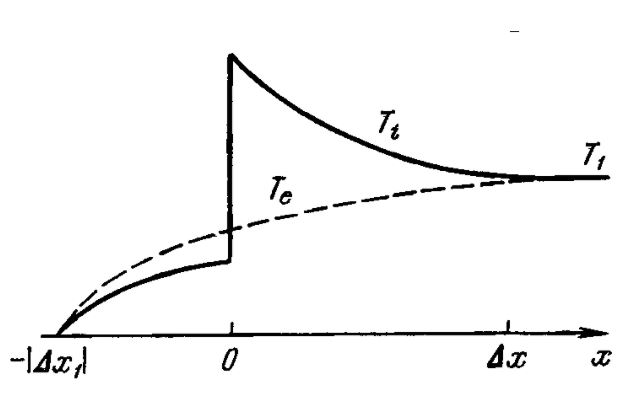
\includegraphics[height=0.15\textheight]{13. teploprov.JPG}
			\caption{Профили ионной и электронной (пунктир) температур во фронте ударной волны с учётом электронной теплопроводности для холодной плазмы~\cite{zeldovich}}
			\label{fig:shock_wave_T_diff} 
		\end{minipage}
	\end{center}
\end{figure}

\subsection{Скачок уплотнения}

Скачок уплотнения -- зона быстрой релаксации, в отличие от понятия ``фронта ударной волны'',
который включает в себя всю переходную область от начального до конечного термодинамически равновесного состояния.

Необратимость ударного сжатия свидетельствует о том, что в нем участвуют диссипативные процессы: вязкость и теплопроводность, которые и приводят к росту энтропии. Именно благодаря вязкости осуществляется необратимое превращение в тепло значительной части кинетической энергии газодинамического потока, набегающего на разрыв в системе координат, где разрыв покоится.

Поскольку процесс ударного сжатия в скачке уплотнения происходит на расстояниях, соизмеримых с газокинетическим пробегом молекул, при изучении структуры скачка следовало бы, строго говоря, исходить из представлений молекулярно-кинетической теории газов. Чтобы не усложнять рассмотрение несущественными в данном случае деталями,
связанными с замедленным возбуждением непоступательных степеней свободы
газа, будем считать газ одноатомным и пренебрегать ионизацией. Запишем уравнения одномерного течения вязкого и теплопроводного газа, стационарного в системе координат, связанной с фронтом волны [уравнение непрерывности, импульса и энтропийное]: 

\begin{align*}
	&\dv{(u\rho)}{x} = 0; \\
	&\dv{}{x}\left(p+u^2\rho-\frac{4}{3}\mu\dv{u}{x}\right)=0; \\
	&uT\rho\dv{\Sigma}{x} = \frac{4}{3}\mu \left(\dv{u}{x}\right)^{2}-\dv{S}{x},
\end{align*}

\begin{align*}
	&\dv{(u\rho)}{x} = 0; \\
	&2u\rho\dv{u}{x}+\dv{p}{x}-\dv{}{x}\frac{4}{3}\mu\dv{u}{x}=0; \\
	&uT\rho\dv{\Sigma}{x} = \frac{4}{3}\mu \left(\dv{u}{x}\right)^{2}-\dv{S}{x},
\end{align*}

где $\Sigma$ -- удельная энтропия; $\mu$ -- коэффициент вязкости; $S$ -- негидродинамический поток энергии, равный в случае теплопроводности $S=-\kappa \frac{dT}{dx}$, где $\kappa$ -- коэффициент теплопроводности.

Преобразуя третье уравнение с помощью второго закона термодинамики: 

\begin{equation*}
	T \Sigma = \dd{\epsilon}+p\dd{V} = \dd{w}-\frac{1}{\rho} \dd{p} 
\end{equation*}

И интегрируя все уравнения, получаем первые интегралы системы (фактически -- законы сохранения):

\begin{align*}
	&\rho u = \rho_0 D; \\ 
	& p+\rho u^{2} - \frac{4}{3} \mu \dv{u}{x} = p_0 + \rho_0 D^{2}; \\
	& w + \frac{u^{2}}{2} + \frac{1}{\rho_0 D} (S - \frac{4}{3} \mu u \dv{u}{x}) = w_0 + \frac{D^{2}}{2}.
\end{align*}

Из этих соотношений следует, что скачок энтропии в ударной волне $\Sigma_1-\Sigma_2 = \Sigma(p_1, \rho_1)-\Sigma(p_0, \rho_0)$ совершенно не зависит ни от механизма диссипации, ни от величины коэффициентов вязкости $\mu$ и теплопроводности $\varkappa$, которые лишь определяют толщину фронта ударной волны.

Система уравнений даёт кривую на плоскости $(p, V)$, вдоль которой происходит превращение газа из начального состояния в конечное. Если ввести безразмерную величину $\eta = \frac{u}{D} = \frac{V}{V_0} = \frac{\rho_0}{\rho}$, то её уравнение -- это

\begin{equation*}
	\frac{p}{p_0}=\frac{1 + \frac{M^{2}}{3} (1-\eta^{2})}{\eta}=\frac{4 \eta_1 - \eta^{2}}{(4 \eta_1 -1) \eta},
\end{equation*}

где $\eta_1 = \frac{1}{4}+\frac{5}{4} \frac{p_0}{\rho_0 D^{2}}= \frac{1}{4} + \frac{3}{4} \frac{1}{M^{2}}$; $M=\frac{D}{c_0}$ -- число Маха, $c_0$ -- скорость звука в начальном состоянии. На рис.~\ref{fig:shock_front} изображены ударная адиабата и кривая, вдоль которой
меняется состояние частицы в волне (а также характерная прямая, связывающая начальное и конечное состояния).

Оценить ширину фронта можно как~\cite{zeldovich}:

\begin{equation*}
	\delta = \frac{D-u_1}{\left(\dv{u}{x}\right)_{max}} \sim l_0 \frac{M}{M^{2}-1},
\end{equation*}

где $l_0$ -- длина свободного пробега. Применимость: $\delta<l$.

\subsection{Релаксационный слой}

Для возбуждения некоторых степеней свободы газа часто требуется много соударений молекул, причем необходимые числа соударений, т. е. времена релаксации, для разных степеней свободы могут сильно различаться.

Время установления полного термодинамического равновесия во фронте ударной волны, а следовательно, и ширина фронта определяются наиболее медленным из релаксационных процессов. При этом следует принимать во внимание только те процессы, которые приводят к возбуждению степеней свободы, дающих заметный вклад в теплоемкость при конечных параметрах газа. Если $\tau_{max}$ — наибольшее время релаксации, $D$ -- скорость фронта ударной волны, а $u_1$ — скорость движения газа за фронтом относительно самого фронта, то ширина фронта порядка $\Delta x\sim u_1\tau_{max}=D(\rho_0/\rho_1) \tau_{max}$.

При комнатных температурах вращения в молекулах возбуждаются также быстро, в результате небольшого числа соударений; колебания же при этих температурах обычно не играют роли. Следовательно, ширина фронта слабых ударных волн, распространяющихся по молекулярному газу, нагретому до комнатной температуры, порядка нескольких газо-кинетических пробегов. 

При температурах порядка $1000^\circ K$, когда величина $T$ сравнима с энергией колебательных квантов молекул $h\nu_{osc}$, возбуждение колебаний требует многих тысяч, а иногда десятков и сотен тысяч соударений. Ширина фронта ударной волны соответствующей амплитуды определяется временем релаксации для колебательных степеней свободы. 

Диссипативные процессы -- вязкость и теплопроводность -- играют роль только в области больших градиентов гидродинамических величин, т. е. в зоне, где возбуждаются быстро релаксирующие степени свободы. Эта зона в какой-то мере совпадает с областью вязкого скачка уплотнения. В зоне медленной релаксации, растянутой на расстояния многих газокинетических пробегов, градиенты малы и диссипацией можно пренебречь.

В данном случае имеется 2 адиабаты (см. рис.~\ref{fig:shock_wave_pV}). Одна из них ($I$) соответствует достижению полного термодинамического равновесия, т. е. соответствует конечным состояниям газа за фронтом ударной волны. Другая ()$II$) соответствует возбуждению только быстро релаксирующих степеней
свободы и ``замороженности'' медленно релаксирующих.

Поскольку в релаксационной зоне удельная энтальпия почти неизменна, а теплоемкость по мере возбуждения ранее замороженных степеней свободы возрастает, температура в ней уменьшается. Уменьшение температуры может быть довольно значительным, если запаздывающая часть теплоемкости велика и вносит большой вклад в конечную теплоёмкость газа. Конечная температура $T_1$ может быть в два-три раза меньше температуры $T$ за скачком уплотнения. Точно так же значительно может возрастать и плотность газа (грубо говоря, $p \sim \rho T$; $p$ меняется слабо, а $T$ -- сильно). Профили $p$, $\rho$, $u$, $T$ во фронте ударной волны, распространяющейся по газу с замедленным возбуждением части теплоемкости, изображены схематически на рис.~\ref{fig:shock_wave_profiles}.

\begin{figure}[ht]
	\begin{center}
		\begin{minipage}[ht]{0.32\linewidth}
			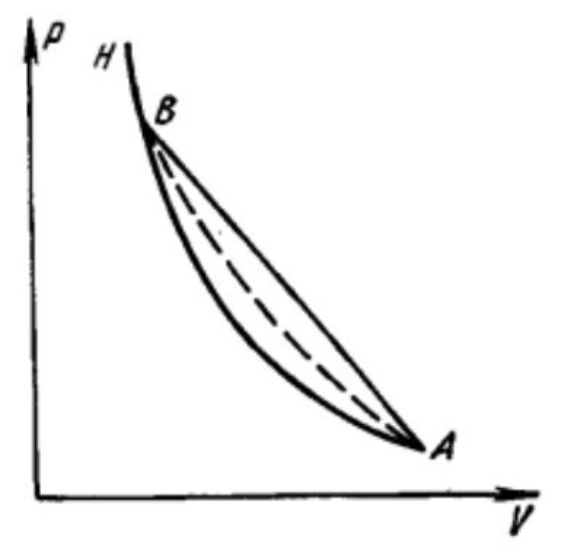
\includegraphics[height=0.2\textheight]{shock_front}
			\caption{Ударный переход $A\rightarrow B$ на $(p, V)$-диаграмме. $H$ -- ударная адиабата. Точка, описывающая состояние внутри фронта волны, пробегает из $A$ в $B$ по пунктирной кривой~\cite{zeldovich}}
			\label{fig:shock_front} 
		\end{minipage}
		\hfill
		\begin{minipage}[ht]{0.32\linewidth}
			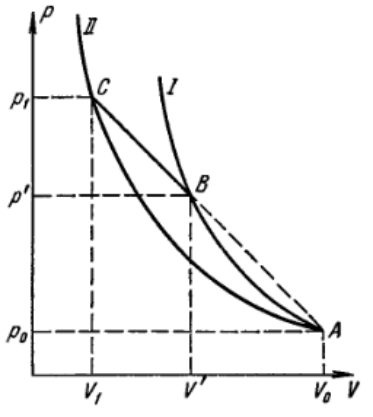
\includegraphics[height=0.2\textheight]{shock_wave_pV}
			\caption{$(p, V)$-диаграмма для ударной волны, распространяющейся по газу с замедленным возбуждением части степеней свободы~\cite{zeldovich}}
			\label{fig:shock_wave_pV} 
		\end{minipage}
		\hfill
		\begin{minipage}[ht]{0.32\linewidth}
			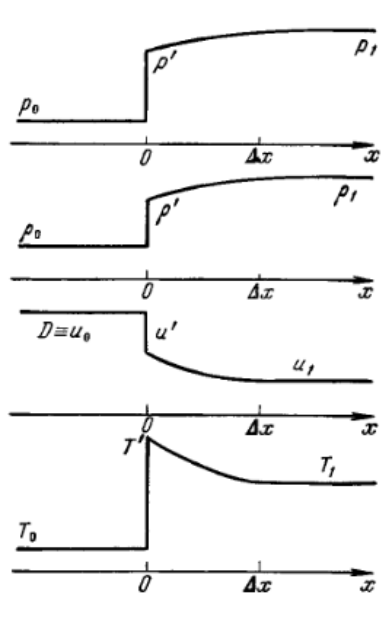
\includegraphics[height=0.2\textheight]{shock_wave_profiles}
			\caption{Профили давления, плотности, скорости и температуры во фронте ударной волны, распространяющейся по газу с замедленным возбуждением части степеней свободы; $\Delta x\approx u\tau_{relax}$ -- ширина фронта~\cite{zeldovich}}
			\label{fig:shock_wave_profiles} 
		\end{minipage}
	\end{center}
\end{figure}

\subsection{Излучение ударных волн, нелинейные волны теплопроводности}

В ударных волнах небольшой амплитуды лучистые давление и энергия гораздо меньше давления и энергии вещества и потому почти не влияют на параметры за фронтом. Иной порядок имеет соотношение потоков энергии излучения и вещества, так как скорости ударных волн, с которыми реально приходится иметь дело, на много порядков меньше скорости света. Отношение потоков энергии $\sigma T^4/(D\rho\varepsilon)(c/D)$, грубо говоря, в $c/D$ раз больше отношения плотностей энергии. В воздухе нормальной плотности, например, оба потока становятся одинаковыми уже при температуре $T\sim300000^\circ$ K, при которой плотность излучения еще очень мала.

На самом деле потери энергии на излучение с поверхности фронта волны весьма ограничены и их эффект обычно незначителен. Дело в том, что в непрерывном спектре газы прозрачны лишь для сравнительно малых квантов. Атомы и молекулы сильно поглощают кванты, энергия которых превышает потенциал ионизации и которые вызывают фотоэффект, а молекулы, как правило, поглощают даже меньшие кванты. При высокой температуре за фронтом энергия, заключенная в области малых частот, составляет лишь небольшую долю от полной энергии спектра. При этом малые кванты находятся в рэлей-джинсовской части спектра и их поток, т. е. возможные потери энергии, во всяком случае пропорциональны не четвертой, а только первой степени температуры.

Таким образом, существование теплового излучения мало сказывается на параметрах газа за фронтом ударной волны не слишком большой амплитуды. Другое дело -- влияние излучения на строение самого фронта ударной волны. Хотя поток излучения, уходящий с фронта волны на ``бесконечность'', весьма мал и не оказывает никакого энергетического влияния на параметры ударной волны, тот факт, что он существует, имеет огромное значение, так как позволяет наблюдать волну оптическими методами. Вопрос о свечении ударной волны и яркости поверхности фронта тесно переплетается с вопросом о структуре фронта~\cite{zeldovich}.

Обычно длина пробега квантов на несколько порядков больше газокинетического пробега частиц и больше ширины релаксационного слоя, где устанавливается термодинамическое равновесие в самом веществе. Ширина фронта ударной волны, в которой лучистый теплообмен играет существенную энергетическую роль, определяется длиной пробега света -- самым большим масштабом длины. В каком-то смысле можно говорить о релаксации излучения во фронте ударной волны, об установлении равновесия излучения с веществом за фронтом.

В предельном случае достаточно слабой волны, когда энергетическая роль излучения мала, профили всех величин в ударной волне имеют характер ``классических'' ступенек (рис.~\ref{fig:shock_wave_classic_profiles}). При возрастании амплитуды быстро растет поток излучения с поверхности фронта $\sigma T_1^4$. Излучение поглощается перед разрывом на расстоянии порядка пробега квантов и нагревает газ, причем нагревание спадает по мере удаления от разрыва вследствие поглощения потока излучения. Скачок уплотнения распространяется теперь не по холодному, а по нагретому газу и температура за скачком $T_{+}$ выше, чем в отсутствие нагревания, т. е. выше, чем в конечном состоянии. За скачком уплотнения температура уменьшается от $T_{+}$ до $T_1$. Другими словами, частица газа, протекающая через ударную волну, сначала нагревается излучением, а испытав ударное сжатие, охлаждается, высвечивая часть энергии, которая и идет на создание потока излучения. Нагревание газа перед разрывом приводит к повышению его давления и некоторому сжатию (а также торможению в системе координат, где фронт покоится). В скачке уплотнения газ сжимается до плотности несколько меньшей конечной. Охлаждение газа за скачком уплотнения способствует его дальнейшему сжатию до конечной плотности. Давление при этом возрастает. Профили температуры, плотности и давления в волне, отвечающие описанной картине, изображены схематически на рис.~\ref{fig:shock_wave_radiation_profiles}.

Температура прогревания перед разрывом $T_{-}$ пропорциональна потоку излучения, выходящего с поверхности разрыва -- $S_0\approx\sigma T_1^4$, и потому быстро увеличивается с возраста- возрастанием амплитуды волны. Соответственно увеличивается превышение температуры за скачком $T_{+}$ над конечной $T_1$ (грубо говоря, $T_{+}-T_1\approx T_{-}$).

При некоторой температуре за фронтом $T_1=T_{cr}$ температура прогревания $T_{-}$ достигает величины Ту и профиль температуры приобретает вид, показанный на рис.~\ref{fig:shock_wave_critical_profiles}. Эта температура $T_{cr}$ может быть названа критической, так как разделяет два существенно различных случая структуры фронта ударной волны.

На самом деле энергия, отбираемая излучением от газа, нагретого в скачке уплотнения, затрачивается на прогревание более толстых слоев перед разрывом. Кванты, выходящие из-за поверхности разрыва, поглощаются перед разрывом в слое порядка длины пробега, а нагретое при этом до температуры, близкой к $T_1$, вещество само излучает, нагревая соседние слои, и т. д. Перед разрывом распространяется \uline{нелинейная теплопроводностная волна}, захватывающая тем более толстый слой газа, чем больше амплитуда ударной волны.

\begin{figure}[ht]
	\begin{center}
		\begin{minipage}[ht]{0.32\linewidth}
			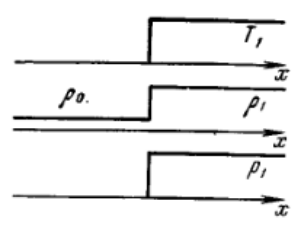
\includegraphics[width=1\linewidth]{shock_wave_classic_profiles}
			\caption{Профили температуры, плотности и давления в ``классической'' ударной волне~\cite{zeldovich}}
			\label{fig:shock_wave_classic_profiles} 
		\end{minipage}
		\hfill
		\begin{minipage}[ht]{0.32\linewidth}
			\begin{center}
			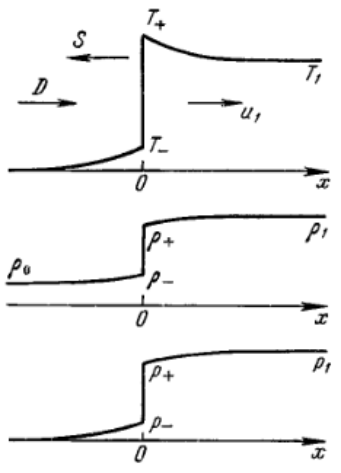
\includegraphics[width=0.6\linewidth]{shock_wave_radiation_profiles}
			\end{center}
			\caption{Профили температуры, плотности и давления
во фронте ударной волны не
слишком большой амплитуды
при учете лучистого теплообмена~\cite{zeldovich}}
			\label{fig:shock_wave_radiation_profiles} 
		\end{minipage}
		\hfill
		\begin{minipage}[ht]{0.32\linewidth}
			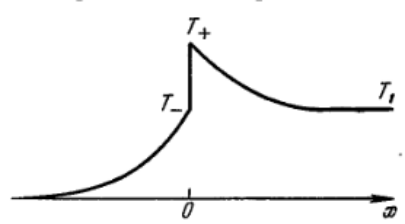
\includegraphics[width=1\linewidth]{shock_wave_critical_profiles}
			\caption{Профиль температуры в
ударной волне ``критической'' амплитуды~\cite{zeldovich}}
			\label{fig:shock_wave_critical_profiles} 
		\end{minipage}
	\end{center}
\end{figure}

\subsection{Токовые слои}

\uline{Токовыми слоями} (ТС) будем называть области столкновительной МГД-плазмы с усиленным током или, что то же самое, поле, масштаб которого значительно меньше типичного, в котором происходит эффективная диссипация~\cite{vainshtein}.

Толщину ТС будем обозначать $\delta$, на этом масштабе меняется поле. Количественной характеристикой ТС может служить время диссипации поля в ТС: $t_0 = \delta^2/\eta$ ($\eta$ -- коэффициент диффузии магнитного поля (магнитная
вязкость), которое можно сравнить с альфвеновским: $t_A = L/c_A$ ($L$ -- характерный масштаб поля). 

Если эти времена одинаковы, то

\begin{equation*}
	\delta = \frac{L}{\sqrt{L_m}},
\end{equation*}

где $L_m = \frac{c_AL}{\eta}$ -- число Лундквиста. Условие наличия ТС: $L<\delta$. Число $L_m$ обычно очень велико (например, для солнечной короны $L_m=10^{11}$). В бесстолкновительной плазме параметр $\delta$ смысла не имеет!

Вынужденное формирование ТС более или менее очевидно: имеются какие-нибудь внешние силы, сближающие магнитные поля противоположных знаков. Другой способ формирования ТС -- самопроизвольный, спонтанный. Он более интересен и важен для приложений. При этом ТС образуется за счет электромагнитных сил. Иначе говоря, магнитные поля устроены таким образом, что пондеромоторные силы стремятся сблизить поля противоположных знаков.

Условие спонтанного формирования ТС -- т.н. приближение сильного поля ($c_A \gg u$, $c_A \gg c_s$ -- скорости звука):

\begin{equation*}
	M_A = \frac{c_A}{u} \gg 1;\;\frac{\rho u^2}{2} \gg \frac{B^2}{8\pi},
\end{equation*}

где $M_A$ -- альфвеновское число Маха.

\section{Прикладные проблемы физики плазмы}

\subsection{Управляемый термоядерный синтез}

дейтерий + тритий = альфа-частица + нейтрон + 17.6 МэВ

[Кенро Миямото, Основы Физики Плазмы и управляемого термоядерного синтеза, Москва, физматлит 2007]

Всем известно про дефект масс, что при слиянии ядер до Fe и Ni выделяется энергия.
основная реакция D+T-> 4He + n [17.59 MeV], 1/5 энергии приходится на He и 4/5 на n
Чтобы сблизить ядра на достаточное расстояние надо преодолеть кулоновский барьер. ту силу, с которой они отталкиваются ($Z_{alpha}Z_p e^2/r_N$) вычислили, что примерное расстояние $r_{n}=1.4*10^{-13}*(A^{1/3}_{\alpha}+A^{1/3}_{\beta}) [cm]$ Но это оказалось слишком мало, ибо не сходилось с вычислениями T солнца, для 10кэВ вычислили точку остановки $R_t=10^{-11} [cm]$

[Миямото стр. 23]

Почему вообще надо удерживать плазму, какие характерные времена? Критерий Лоунсена 
Дело обстоит в том, что система должна сама себя поддерживать и при этом отдавать эл. энергию. Энергия в единице объёма $(3/2)nk(T_i+T_e)$. Время остывания $\tau_E = \frac { (3/2)nk(T_i+T_e) }{P_L+R}$, , где $P_L$ и $R$ соответственно мощность потерь энергии на диффузию и излучение плазмой. В то же время, в объёме происходит выделение тепла за счёт термоядерного синтеза мощностью. $P_{NF}=(n/2)(n/2)<\sigma v> Q_{NF} $. Потому
 как D и T присутствуют в реакторе в равном количестве и концентрация каждого n/2 соответственно. $<\sigma v> $ - вероятность процесса,   $Q_{NF} $ энергия на одну реакцию.
Чтобы всё было устойчиво и не затухало: $P_{heat}=P_L + R = \frac{3nkT}{\tau_E} < \eta_{el} \eta_{heat} P_{NF} $, где $\eta_{el} $ - КПД получения эл. мощности ,$ \eta_{heat} $ - КПД нагрева.

Итого: $ \frac{3nkT}{\tau_E} < \eta_{el} \eta_{heat} Q_{NF} n^{2} \frac{<\sigma v>}{4}$

\begin{equation}
	n \tau_E > \frac{12 kT}{\eta Q_{NF} <\sigma v>} > 1.7*10^{20} m^{-3} s
\end{equation}
 - Критерий Лоунсена , критерий термоядерности. То есть надо или увеличивать концентрацию, или время удержания. Поэтому есть как токамаки с непрерывным временем работы, так и импульсные(импульсно поддерживается магнитное поле).
Понятно, что чем горячее плазма, тем труднее её удерживать, понятно что удерживать надо именно магнитным полем.

\subsection{Магнитное удержание}

Уравнения магнитной гидродинамики тут написаны [Голант Жилинский Сахаров, Основы ФП,  §10.1]

Из уравнения для средней скорости $\rho (du/dt)=(1/c)[j H]-grad\;p$; где $p=p_e+p_i$ - суммарное давление, $j=en(u_i+u_e)$ - плотность тока, $ du/dt=\delta u / \delta t + (u grad)u$ полная производная

можно вывести условие равновесия
\begin{equation}
	\frac{1}{c}[j H]=grad\;p
\end{equation}
[Голант Жилинский Сахаров, Основы ФП,  §10.2]


Идея состоит в том, что преодолеть давление плазмы как газа с ооочень большой температурой с помощью давления магнитного поля около стенок.
Первая задача, возникающая при рассмотрении удержания плазмы в магнитном поле, заключается в определении условий, при которых достигается равновесие, т. е. электродинамические силы, действующие на каждый элемент объема плазмы, уравновешивают градиент давления.
\begin{equation}
	G_H=\frac{1}{c} [j H]=\frac{1}{4 \pi} [H rotH]=-\frac{1}{8 \pi} grad(H^{2})+\frac{1}{4 \pi} (H grad) H
\end{equation}
Так же есть отдельный случай, когда линии имеют радиус кривизны R.

\begin{equation}
(\vec H grad)\vec H=H(\vec h grad)\vec h H=H^{2} grad_{||}\vec h + \frac{1}{2} grad_{||} H^{2}=-H^{2} \frac{\vec R}{R}+\frac{1}{2} grad_{||} H^{2}
\end{equation}


, где $\vec h= \frac{\vec H}{H}$; $grad_{||}=(\vec h \; grad)$ - проекция градиента на направление магнитного поля. Подставляем в предыдущее выражение и получаем, что давление:
\begin{equation}
 G_H=-grad_{\perp}(H^{2}/8\pi)-(H^{2}/4\pi R^{2})\vec R
\end{equation}
Первое слагаемое в представляет собой поперечный градиент введённого магнитного давления. Действие этой силы можно описать как взаимное «расталкивание» силовых линий в поперечном направлении. Второе слагаемое определяет силу, направленную к центру кривизны силовых линий, и называется натяжением магнитного поля. Оно формально получается, если приписать силовым линиям свойства растянутой струны.

Для равновесия: 
\begin{equation}
 grad p + grad_{\perp}(H^{2}/8\pi)+(H^{2}/4\pi R^{2})\vec R =0
\end{equation}

Для случая, когда силовые линии прямые ($R\rightarrow \inf $), уравнение сводится к постоянству суммы кинетического и магнитного давлений в плоскости, перпендикулярной магнитному полю:
\begin{equation}
p + H^{2}/8\pi=const
\end{equation}
\begin{equation}
p_0 + H_{0}^{2}/8\pi=H_{e}^{2}/8\pi
\end{equation}

Равенство показывает, что максимальное давление плазмы, которое можно удерживать магнитным полем, равно магнитному давлению вне плазмы $H_{e}^{2}/8\pi$. При описании магнитного удержания часто вводят коэффициент $\beta$, представляющий собой
отношение давления удерживаемой плазмы к максимально возможному: $\beta=p/p_{max}=8\pi p/H_{e}^{2}$
Но это удержание поперёк линий магнитного поля, а строить комплексы в виде торов не всегда удобно, поэтому было придумано пробочное удержание.

пробочное удержание [Миямото стр. 32]

Понятно, что всё движение электрона в магнитном поле можно описать как движение вдоль и поперёк поля. Вдоль - свободное движение, поперёк - ларморовское вращение.
Если рассмотрим электрон в поле, он будет вращаться по кругу с радиусом равному Ларморовскому. Его можно представить в виде витка с током. У витка с током есть магнитный момент.
\begin{equation}
 \mu=I*S=\frac{q\Omega}{2\pi} * \pi \frac{\rho^{2}}{2}=\frac{mv_{perp}^{2}}{2B}
\end{equation}	
Но кин энергия должна сохранятся при движении в магнитном поле, поэтому электрон будет лететь вдоль поля пока
\begin{equation}
	\frac{mv_{||}^{2}}{2}+\frac{mv_{\perp}^{2}}{2}=\frac{mv^{2}}{2}=const
\end{equation}	
Поскольку магнитный момент сохраняется, то:
\begin{equation}
 v_{||}=+-(\frac{2}{m}E-v_{\perp}^{2})^{1/2}=+-(v^{2}-\frac{2}{m} \mu B)^{1/2}
\end{equation}	
То есть электрон может полностью убрать продольную скорость и отразиться. Почему возникает этот эффект ? Потому что на магнитный диполь действует сила $-\mu \grad_{||}$ B. Ну и вводится пробочное отношение - отношение магнитных полей в центре и на краях ловушки $R_M=\frac{B_M}{B_0}$


\subsection{Плазменные источники излучения}

раздел физики плазмы, изучающий коллективные взаимодействия плотных потоков (пучков), приводящие к возбуждению в системе линейных и нелинейных волн и колебаний, и использование эффектов такого взаимодействия.
плазменные ускорители, основанные на явлении коллективного ускорения тяжёлых частиц электронными пучками и волнами в плазме

плазменно-пучковый разряд, основанный на коллективном механизме взаимодействия плотных пучков заряженных частиц с газом;

турбулентный нагрев плазмы плотными пучками аряженных частиц и коллективных процессов при транспортировке и фокусировке пучков в проблеме управляемого термоядерного синтеза (УТС)

[Богданкевич Л С, Кузелев М В, Рухадзе А А "Плазменная СВЧ электроника" УФН 133 3–32 (1981)]
DOI: 10.3367/UFNr.0133.198101a.0003
URL: https://ufn.ru/ru/articles/1981/1/a/

Когда говорят о сильноточных электронных пучках, то прежде всего имеют в виду пучки с током, превышающим так называемый предельный вакуумный ток. Известно, что в металлическом волноводе с радиусом R и длиной $L >> R$, который обычно используется в вакуумной электронике в качестве резонатора, ток пучка ограничен пространственным зарядом электронов, причем предельный ток по порядку величины определяется соотношением:
\begin{equation}
	\omega_{b \; vol}^{2} \approx \frac{c^{2}}{S} \gamma
\end{equation}
, где $\gamma = [1-(u^{2}/c^{2})]^{-1/2}$ - — релятивистский фактор энергии электронов, $S$ — поперечное сечение пучка, меньшее или порядка сечения волновода, а $\omega_{b}=\sqrt{4\pi e^{2} n_{b} /m}$ — лэнгмюровская частота электронов пучка. 


Следовательно, сильноточным следует считать пучок, в котором $\omega_{b}^{2}>\omega_{b\;vol}^{2}$. Такой пучок может распространяться в волноводе только при наличии нейтрализации пространственного заряда электронов, что достигается заполнением системы относительно плотной (по сравнению с плотностью пучка) плазмой. Таким образом, сильноточная СВЧ электроника, строго говоря, может быть только плазменной. При этом, однако, плазма может и не влиять существенным образом на частоты генерируемых пучком электромагнитных волн. Дело в том, что длины волн возбуждаемых пучком электромагнитных колебаний меньше или порядка поперечных размеров электродинамической системы генератора, т. е. резонатора, точнее $\omega>\omega_{crit}= \mu c/R$, где $\mu$ характеризует радиальное волновое число моды колебаний (корни функций Бесселя или ее производных); обычно $\mu \sim 3-10$. Если плазма, заполняющая резонатор, имеет относительно низкую плотность, так что $\omega_{pl}=\sqrt{4\pi e^{2} n_{p} /m} < \mu c/R$ , то она существенно не меняет электродинамику резонатора, который по своим электродинамическим свойствам остается практически вакуумным. Вместе с тем такая плазма может нейтрализовать пространственный заряд пучка и позволить пропустить через резонатор сильноточный пучок со сверхпредельным током. Однако ток пучка при этом ненамного может превышать предельный, не более, чем в $\mu^{2} S/\gamma R^{2}$ раз, что следует из неравенств $\omega_{b}^{2}<\omega_{p}^{2}<\mu^{2} c^{2}/R^{2}$.

Иное положение имеет место в случае достаточно плотной плазмы, когда $\omega_{pl}>\mu c/R$. Роль такой плазмы в резонаторе не ограничивается нейтрализацией пространственного заряда пучка, она существенно меняет всю электродинамику резонатора и, в частности, спектры частот собственных электромагнитных мод резонатора. Именно в этом случае мы имеем дело с настоящей плазменной электроникой, которая, как будет видно из дальнейшего, позволяет продвинуться в область токов электронного пучка, намного превосходящих предельный вакуумный ток, вплоть до $\mu^{2}\gamma S/R^{2}$ раз. Более того, с помощью ультрарелятивистских электронных пучков в таких системах оказывается возможным эффективное возбуждение колебаний с длиной волны, намного меньшей поперечных размеров резонатора $\lambda \approx R/\gamma^{2}$ .

\begin{figure}[ht]
	\begin{center}
		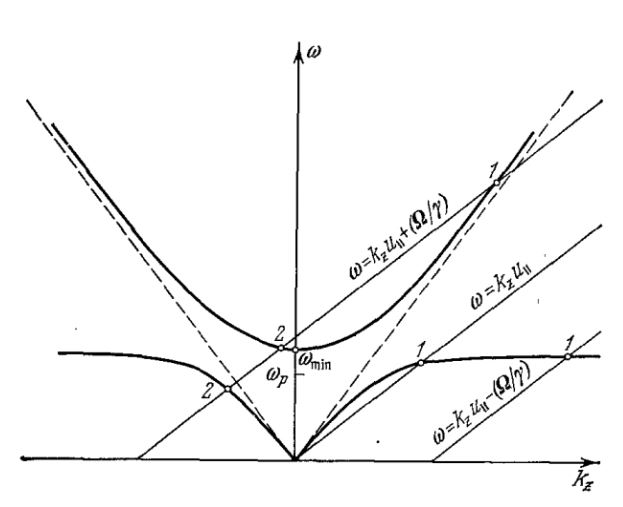
\includegraphics[width=70mm]{dispers_14_3.JPG}
	\end{center}
\end{figure}

Другими словами, плазменная СВЧ электроника открывает возможиость создания коротковолновых источников мощного электромагнитного излучения.


Без формул, наверное сразу можно нарисовать дисперсионку резонатора, без пучка.  Как мы видим при добвалении плазмы, появилась ещё одна нижняя ветвь. Точки 1. это работа в режиме усилителя. Пучок (наклонные линии $\omega=ku\pm (\Omega/\gamma)$) усиливает волну бегущую в ту же сторону. Точки 2. это работа в режиме генератора. Пучок усиливает встречную волну.



плазменная СВЧ электроника.
Компрессоры импульсов.


\subsection{Преобразование тепловой энергии в электрическую: МГД-преобразователи, тепловые преобразователи}

[райзер, дополнение, стр. 673]

\begin{figure}[ht]
	\begin{center}
		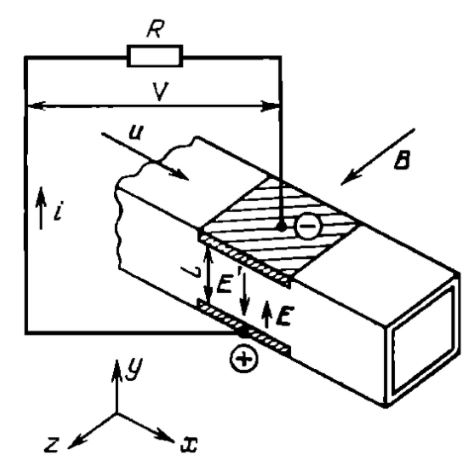
\includegraphics[width=70mm]{MGD_generator.JPG}
	\end{center}
\end{figure}

Принцип работы МГД генератора представлен на рисунке. Ионизованный газ протекает по каналу со скоростью и и пересекает линии напряженности приложенного постоянного магнитного поля. В движущейся среде индуцируется электрическое поле $E' =\frac{1}{c} [V\; B]$. Вектор магнитной индукции $B =\mu H$ не отличается от $H$, поскольку магнитная проницаемость газа $\mu=1$. Направление Е' характеризуется  
координатным равенством $E'_y=-u_x B_z / c $. Индуцированное поле Е' движет электроны вверх. У верхней  
стенки канала накапливается отрицательный пространственный заряд, у нижней — положительный. Если внешняя цепь между электродами, помещенными на этих стенках, разомкнута, заряды накапливаются, пока созданное ими электрическое поле $E_{\inf}$ не уничтожит индуцированное ($E_{\inf}=-E'$). Потенциал нижнего электрода при этом превышает потенциал верхнего на $V_{\inf} = E_{inf} L$. Это напряжение совпадает по величине с ЭДС генератора:
\begin{equation}
	\varepsilon=E'_{y}L=(-u_x /c)(B_z L)
\end{equation}

Если цепь замкнуть через нагрузочное сопротивление и обеспечить достаточно высокую электронную эмиссию с нижнего электрода, например путем его активирования и нагревания, в цепи потечет ток. Реально электроны в газе непрерывным потоком дрейфуют вверх, исходя из нижнего положительного электрода, который в отличие от обычного разряда работает подобно катоду, и внедряясь в верхний. Частичное устранение приэлектродного пространственного заряда, уносимого током, приводит к уменьшению напряжения на электродах $V= E_{y} L$ по сравнению с $V_{inf}=|\varepsilon|$. В пренебрежении эффектом Холла, в результате которого возникает ток по оси $x \perp E, B$, плотность тока в газе:
\begin{equation}
	j=\sigma(E+E')=\sigma(E+\frac{1}{c}[u\;B])
\end{equation}

Ну или в нашей системе координат 
\begin{equation}
	j_y=\sigma(E_y-\frac{[u\;B]}{c}) <0
\end{equation}

Дело ещё обстоит в том, что ток в цепи как раз и зависит от E меж электрожного промежутка, как $i*R=V$ (общий ток через систему с площадью $S$, $i=j*S$), в то время как $V=E*L$, то есть мы получили систему самосогласованных уравнений, которые замкнулись сами на себя. А именно:
\begin{equation}
	i=S \sigma(V/L-uB/c)=S \sigma(iR/L-uB/c)
\end{equation}
отсюда можно выразить $i$ в чистом виде. $i=\frac{u\;B}{c(\frac{R}{L}-\frac{1}{\sigma S})}$

При протекании тока на газ действует тормозящая пондеромоторная сила, в результате чего он и теряет энергию. Отношение мощности, выделяемой в нагрузке, к мощности, отбираемой от газа: 
\begin{equation}
	\frac{iV}{(u/c)(jB)LS}=\frac{V}{\varepsilon}
\end{equation}

т. е. электрический КПД генератора тем выше, чем ближе ситуация к режиму разомкнутой цепи. Но абсолютное значение полезной мощности $iV$ максимально, когда сопротивления нагрузки и плазмы одинаковы и $V=|\varepsilon|/2$


\subsection{Химические реакции в равновесной и неравновесной плазме. \textcolor[rgb]{1,0,0}{Механизмы и кинетика осуществления плазмохимических реакций, роль заряженных и возбужденных частиц. Энергетика химических реакций в электрических разрядах}. Закалка продуктов плазмохимических процессов.}
 
[В.Д. Русанов, А.А. Фридман, Физика химически-активной плазмы]

Очевидно, что хотели увеличить скорость некоторых процессов и сократить их количество. Поэтому некоторые реакции хотели провести напрямую в плазме. В рамках классической кинетики при этом экспоненциально ускоряется в соответствии с известным законом Аррениуса $ k \sim exp(-E_{a}/T)$, где $E_a$ — характерная величина энергетического барьера реакции; Т — температура системы. (Понятно, что хим реакция протекает при столкновении двух/трёх частиц, каждая из которых может быть подчинена максвеллу).
 
Резкое повышение скорости процесса может иметь место уже при температурах 3000—5000° С, что значительно выше обычного диапазона температур химических, технологических и  металлургических процессов. Скорость переноса реагентов через зону реакции, очевидно, должна соответствовать повышенной удельной производительности, которая достигается в реакционной зоне при очень высоких температурах, что можно реализовать только в случае газового транспорта реагентов с повышенными скоростями ($5*10^{3}--5*10^{4}$ см/с). 
Очевидно, что подвод к газу столь высокопотенциального тепла не может быть осуществлен с помощью традиционных методов теплопередачи. Сверхвысокие температуры в реакционной зоне должны обеспечиваться подводом энергии электромагнитного поля от внешнего источника, а не тепловой энергии. Этим требованиям отвечает совмещение реакционной зоны с газоразрядной, в которой можно организовать локальный нагрев реагентов до высоких температур за счет активных потерь энергии электромагнитного поля.

Плазмохимические системы в целом можно условно разделить на два больших класса — квазиравновесные и неравновесные.
Температура Т в случае, когда система близка к равновесию (квазиравновесию), является единственной энергетической характеристикой системы, т. е. $T \approx T_{o} \approx T_{e} \approx T_{i} \approx  T_{r} = T_{v}$, где $T_{o}$ — поступательная температура нейтрального газа, $T_e$ — температура электронов; $T_i$ — температура ионов; $T_r$ — вращательная температура молекул; $T_v$— колебательная температура молекулярного газа. 

Если равновесие в системе не достигнуто, то могут реализоваться различные неравновесные (неизотермические) ситуации, из которых наибольший практический интерес с точки зрения оптимизации характеристик реакционной зоны имеют простейшие системы 

\begin{equation}
T_e > T_0, T_i, T_v,T_r
\end{equation}

\begin{equation}
T_e > T_i > T_0  \approx T_v  \approx T_r
\end{equation}

Неравновесность первого типа представляется наиболее универсальной, при этом концентрация электронов в реакционной зоне оказывается существенно ниже, чем определенная формулой Саха по температуре электронов Те, но на много порядков больше величины пе, определенной по этой же формуле для температуры  нейтральных частиц $T_0$. Частный случай неравновесной системы, реализуемой во втором случае, связан не только с отрывом температуры электронов, но также с отрывом колебательной температуры  молекул от вращательной и поступательной температуры газа, который может обеспечить реализацию химических процессов через колебательное возбуждение реагирующих молекул. 

При накачке электронным ударом происходит преимущественное заселение нижних колебательных уровней молекул. Заселение высоковозбужденных состояний, проявляющих химическую активность, происходит в основном за счет обмена колебательными квантами. В результате этого процесса с учетом ангармонизма молекул могут возникать распределения по колебательным состояниям, заметно отличающиеся от больцмановского $f(v) \sim exp(-\hbar \omega \nu / T_v)$, где $\hbar \omega \nu$ - колебательная энергия. Например, для простейшего случая двухатомных молекул учет ангармонизма ($x_e$) приводит к обогащению заселенности высоковозбужденных состояний согласно соотношению Тринора:

\begin{equation}
  f(v) \sim exp(-\frac{\hbar \omega \nu} {T_v}+x_e\frac{\hbar \omega \nu^{2}}{T_0})
\end{equation}

Доля высоковозбужденных реакционноспособных молекул согласно этому соотношению может быть выше больцмановской на много порядков. Соответственно высокими оказываются и скорости плазмохимических процессов. Это позволяет подавить вредное влияние релаксации и обратных химических реакций, обеспечивая в итоге высокую энергетическую эффективность. 

Подробнее остановимся на неравновесных разрядах. [Д.И. Словецкий, механизмы химических реакций в неравновесной плазме]
Именно на практике термин чаще встречается “неравновесный разряд” в отношении возбуждённых частиц. А именно это распространено в создании мощных газоразрядных лазеров. Понятно, что нам энергетически выгодно заселять только тот уровень, который бы потом излучил. С ростом энергии у нас будут сначала будет возбуждаться поступательная степень свободы, потом вращательная и самая последняя - колебательная. И вот иногда, во время столкновений нейтрала с возбуждённой частицей может возбудиться именно колебательная степень свободы, минуя первые две. тем самым, у нас создаётся неравновесное распределение заселённости по уровням.
В таком случае, вообще, надо начинать заного писать кин уравнение для частиц сорта A на уровне i.
\begin{equation}
\frac{\delta [A(i)] f_{A(i)}}{\delta t}+\frac{F_A}{M_A}\frac{\delta [A(i)] f_{A(i)}}{\delta V_A} +v_A \frac{\delta [A(i)] f_{A(i)}}{\delta r}=\sum_{S,n} I(A,i|S,n) 
\end{equation}

Поскольку классическая химическая кинетика имела дело с сумарными концентрациями чатиц определённого сорта, то и в этом случае можно просуммировать концентрации по всем уровням энергии интегрируя по всем скоростям можно получить
 \begin{equation}
-\frac{d [A] }{dt}=k(C,D|A,B) [A][B]-k(A,B|C,D) [C][D]
\end{equation}
В общем случае коэффициенты реакции могут зависеть от всего на свете, они так же могут иметь пороговый характер. И для описания неравновесных процессов обычно выписываются все уравнения для основных уровней всех веществ, участвующих в реакции и решается на компьютере.

[Неравновесная колебательная кинетика, под редакцией М. Капителли, пункт 4, стр 105]

Самые основные процессы в такой плазме $VT$ (колебательно поступательный), $VV$ (колебательно колебательный) обмен энергии. (много непонятной теории)

\subsection{Методы диагностики химически активной плазмы.}

 [словецкий, стр 39]

\subsection{Взаимодействие плазмы с поверхностью твердых тел. Плазменные технологии (травление, имплантация, упрочнение, нанесение покрытий и пр.)}

 [СТЕПАНОВСКИЙ А. С. ИОННАЯ ОБРАБОТКА МАТЕРИАЛОВ ]


В зависимости от параметров ионного или электронного потока в поверхностном слое деталей могут происходить различные процессы. При энергии ионов (уже не инертного газа) $E \approx 10\ldots 100$ эВ на поверхности детали происходит конденсация ионов. Такая обработка используется для осаждения покрытий. Если $E \approx 10^2\ldots10^3$ эВ, то реализуется процесс ионного распыления (травления), который применяется для очистки поверхностей деталей, активирования поверхностного слоя, формирования микрорельефа. При $E > 10^4$ эВ происходит ионная имплантация, т.е. внедрение ионов имплантируемого вещества в поверхностный слой детали. Таким образом, можно модифицировать поверхностный слой путем его легирования практически любыми элементами. Имплантация приводит к увеличению концентрации дефектов в облучаемом материале, которые в этом случае называют радиационным. При больших дозах облучения поверхностного слоя детали становятся аморфными из-за высокой концентрации радиационных дефектов. Ионная бомбардировка и облучение электронами приводит к нагреву поверхностного слоя, а в ряде случаев наблюдается образование газовых пузырьков и микропор, которые приводят к уменьшению плотности материала


При плазменном травлении обрабатываемый образец помещается непосредственно в область химически активной плазмы, располагаясь на специальном подложкодержателе, и
находится обычно под плавающим потенциалом. Основными частицами, участвующими в процессе плазменного травления и влияющими на него, являются свободные атомы, радикалы, ионы и электроны. Вклад этих частиц в плазменное травление различен: химически активные частицы, т.е. свободные атомы и радикалы, вступают в химическую реакцию с поверхностными атомами материалов и удаляют поверхностные слои в
результате образования летучих продуктов реакции, а электроны и ионы активируют эту реакцию, увеличивая скорость травления. Активирующее воздействие ионов и электронов
определяется энергией, с которой они бомбардируют обрабатываемую поверхность. К плазменному травлению относятся процессы, в которых энергия ионов не превышает 100 эВ.

\part{Дополнительная программа}

\section{Кинетический и гидродинамический методы описания плазмы}

\subsection{Уравнение Лиувилля и условия корректного перехода к кинетическому уравнению с самосогласованным полем для одночастичной функции распределения}

Уравнение Лиувилля = уравнение Больцмана в бесстолкновительном приближении -- уравнение, описывающее изменение функции распределения (ФР) частиц плазмы определённого сорта.

Вывод уравнения Лиувилля можно посмотреть перед~\eqref{eq:Liouville_eq}. Приведём здесь его ещё раз:

\begin{equation}
	\frac{df}{dt} = \frac{\partial f}{\partial t} + \frac{d\vec{r}}{dt}\frac{\partial f}{\partial \vec{r}}+ \frac{\vec{F}}{m}\frac{\partial f}{\partial \vec{v}} = 0
\end{equation}

Переход к кинетическому уравнению с самосогласованным полем есть вывод уравнения Власова, см. подраздел~\ref{subsubsec:Vlasov_eq}.

\subsection{Разлет бесстолкновительной плазмы (ограниченной и из полупространства)}

Здесь приведём небольшой вывод для газа из~\cite{silin}. 

Пусть газ занимает \uline{полупространство} $x<0$. Частицы газа распределены по скоростям согласно максвелловскому распределению. Пусть в начальный момент времени $t=0$ удаляется стенка, ограничивающая газ, и он начинает расширяться в пустоту. Для ФР при таком свободно-молекулярном расширении можно записать:

\begin{equation*}
	\pdv{f}{t}+v_x\pdv{f}{x} = 0
\end{equation*}

Очевидно~\cite{silin}, решение уравнения имеет вид $f(x, \vb{v}, t) = F(x-v_xt; \vb{v})$. Поскольку в начальный момент времени распределение частиц описывается максвелловским образом:

\begin{equation*}
	f(x, v, 0) = n_0\left(\frac{m}{2\pi T}\right)^{3/2}e^{-\frac{mv^2}{2T}}\varTheta(-x),
\end{equation*}

где $\varTheta(-x)$ -- степ-функция; то решение уравнения имеет вид

\begin{equation*}
	f(x, v, 0) = n_0\left(\frac{m}{2\pi T}\right)^{3/2}e^{-\frac{mv^2}{2T}}\varTheta(v_xt-x),
\end{equation*}

Тогда концентрация зависит от координат и времени следующим образом:

\begin{multline*}
	n(x, t) = \int\dd{\vb{v}}f(x, \vb{v}, t) = n_0\sqrt{\frac{m}{2\pi T}} \int\limits_{-\infty}^\infty \dd{v_x}e^{-\frac{mv_x^2}{2T}}\varTheta(v_xt-x) = n_0\sqrt{\frac{m}{2\pi T}} \int\limits_{x/t}^\infty \dd{v_x}e^{-\frac{mv_x^2}{2T}} = \\
	= n_0\sqrt{\frac{m}{2\pi T}} \sqrt{\frac{2T}{m}} \int\limits_{\frac{x}{t}\sqrt{\frac{m}{2T}}}^\infty\dd{\xi}e^{-\xi^2} = \frac{n_0}{\sqrt{\pi}}\frac{\sqrt{\pi}}{2}\left\lbrace 1-erf\left(\frac{x}{t}\sqrt{\frac{m}{2T}}\right) \right\rbrace = \frac{n_0}{2}\left\lbrace 1 - erf \left(\frac{x}{t} \sqrt{\frac{m}{2T}}\right) \right\rbrace
\end{multline*}

От $\left(\frac{m}{2\pi T}\right)^{3/2}$ остаётся только $\sqrt{\frac{m}{2\pi T}}$, т.к. были взяты интегралы по $\dd{v_y}$ и $\dd{v_z}$; $erf(x)$ -- функция ошибок/интеграл вероятности. В пределе $x/t\rightarrow-\infty$ плотность газа обращается в $n_0$.

Средняя скорость газа имеет следующий вид:

\begin{multline*}
	v(x, t) = \frac{1}{n(x, t)}\int\dd{\vb{v}}f(x, \vb{v}, t) = \frac{n_0}{n_0(x, t)}\sqrt{\frac{m}{2\pi T}}\int\limits_{x/t}^\infty\dd{v_x}v_xe^{-\frac{mv_x^2}{2T}} = \frac{n_0}{n_0(x, t)}\sqrt{\frac{m}{2\pi T}}\frac{2T}{2m} \int\limits_{\frac{mx^2}{2t^2T}}^\infty\dd{\xi}e^{-\xi} = \\
	= \frac{n_0}{n_0(x, t)}\sqrt{\frac{T}{2\pi m}}e^{-\frac{mx^2}{2t^2T}}
\end{multline*}

Поскольку зависимость плотности частиц и средней скорости от времени и координат определяется комбинацией $x/t$, то их распределения в различные моменты времени подобны и отличаются лишь масштабом вдоль оси $x$, который растет пропорционально времени. Такое движение называется \uline{автомодельным}.

Разберём разлёт \uline{ограниченного} газа. Пусть в момент $t=0$ одна из ограничивающих поверхностей газа расположена при $x=0$, а вторая при $x=-L_0$, имеем для начальной функции распределения выражение:

\begin{equation*}
	f(x,\vb{v}, 0) = n_0\left(\frac{m}{2\pi T}\right)^{3/2}e^{-\frac{mv^2}{2T}}\left(\varTheta(-x)-\varTheta(-x-L_0)\right)
\end{equation*}

Тогда легко аналогично вышенаписанному показать, что концентрация и средняя скорость газа будут равны:

\begin{align*}
	n(x, t) &= \frac{n_0}{2}\left\lbrace erf\left(\frac{x+L_0}{t}\sqrt{\frac{m}{2T}}\right) - erf\left(\frac{x}{t}\sqrt{\frac{m}{2T}}\right) \right\rbrace \\
	v(x, t) &= \frac{n_0}{n_0(x, t)}\sqrt{\frac{T}{2\pi m}}\left\lbrace e^{-\frac{mx^2}{2t^2T}} - e^{-\frac{m(x+L_0)^2}{2t^2T}}\right\rbrace 
\end{align*}

\subsection[Приближенное описание столкновений в рамках кинетического уравнения. Интеграл столкновений в форме Ландау, уравнение Фоккера-Планка, релаксационная форма интеграла 	столкновений ($\tau$-приближение). Кинетическое описание упругих и неупругих столкновений электронов с атомами и молекулами. Приближенное описание кинетики электронов в слабом однородном электрическом поле (расчет эффективной частоты столкновений и нагрева электронов). Явление убегающих электронов]{Приближенное описание столкновений в рамках кинетического уравнения. Интеграл столкновений в форме Ландау, уравнение Фоккера-Планка, релаксационная форма интеграла 	столкновений \linebreak ($\tau$-приближение). Кинетическое описание упругих и неупругих столкновений электронов с атомами и молекулами} \label{subsec:collision_terms}

\subsubsection{Приближенное описание столкновений в рамках кинетического уравнения}

Столкновения в рамках кинетического уравнения описываются с помощью интеграла столкновений (см. формулу~\eqref{eq:Boltzmann_eq}). В целом, больцмановский подход предполагает рассмотрение только парных столкновений и замыкание системы (см. выше приближение Больцмана~\eqref{eq:Boltzmann_relation}). Считаем, что столкновения резко меняют скорости частиц и не нарушают их расположения в пространстве (точечность столкновений). Плазма -- локально однородна, слагаемое в кин. уравнении $\sim \frac{\partial}{\partial \vec{r}}$ можно рассматривать как снос. Изменение скоростей можно рассматривать в отдельности от изменения координат\Tokman.

Пусть выражение (\eqref{eq:Liouville_eq}) записано для частиц сорта $\alpha$ и $\beta$. Будем учитывать в интеграла столкновений соударения между частицами как одного, так и двух разных сортов. Пусть $\Gamma_\alpha$ -- совокупность всех внутренних координат частиц сорта $\alpha$ [в т.ч. -- квантовых чисел = их распределение по уровням; пока мы не определили, упругие или неупругие взаимодействия -- общий случай]. Формально это учитывается в определении концентрации:

\begin{equation*}
	n(\vec{r}, t) = \int\limits_{\infty}f(\Gamma_\alpha,\vec{r},t)dv_\alpha,
\end{equation*}

где $\vec{r}$ -- относительно центра масс данной частицы.

Задача: определить число столкновений частиц определённого сорта в определённом интервале. Столкновения в ``реальном'' пространстве приводят к уходу частиц из одной области фазового ($\Gamma-$) пространства в другую. По сути, отношение числа частиц к объёму и есть ФР.

\begin{figure}[ht]
	\begin{center}
		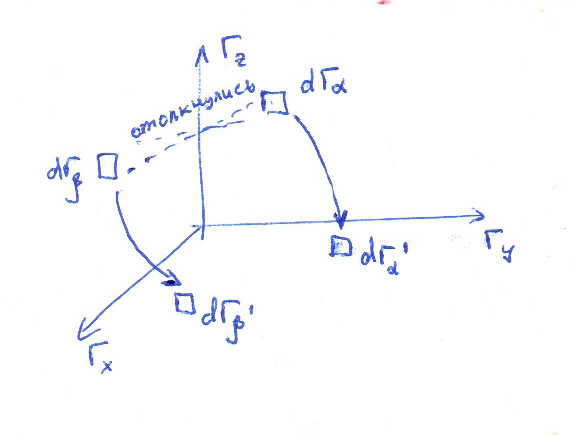
\includegraphics[width=0.45\linewidth]{boltzmann_collision_term.pdf}
	\end{center}
	\caption{Рисунок из лекций}
	\label{fig:boltzmann_collision_term}
\end{figure}

Пришло в объём $d\Gamma_\alpha$:

\begin{equation*}
	dQ_\alpha^{(+)} = d\Gamma_\alpha \int\limits_{\infty}d\Gamma_\alpha^{'} \int\limits_{\infty}d\Gamma_\beta^{'} \int\limits_{\infty}d\Gamma_\beta \cdot f_{\alpha\beta}\left(\Gamma_\alpha^{'} \Gamma_\beta^{'}\right) \cdot \omega_{\alpha\beta}\left(\Gamma_\alpha, \Gamma_\beta, \Gamma_\alpha^{'}, \Gamma_\beta^{'}\right)
\end{equation*}

Ушло из объёма $d\Gamma_\alpha$:

\begin{equation*}
	dQ_\alpha^{(-)} = d\Gamma_\alpha \int\limits_{\infty}d\Gamma_\alpha^{'} \int\limits_{\infty}d\Gamma_\beta^{'} \int\limits_{\infty}d\Gamma_\beta \cdot f_{\alpha\beta}\left(\Gamma_\alpha \Gamma_\beta\right) \cdot \omega_{\alpha\beta}\left(\Gamma_\alpha^{'}, \Gamma_\beta^{'}, \Gamma_\alpha, \Gamma_\beta\right),
\end{equation*}

где выбрано обозначение $\omega_{\alpha\beta}(A, B, C, D)=\omega_{\alpha\beta}(C\rightarrow A, D\rightarrow B)$.

Важно: $\omega(\ldots)\neq 0$ -- только для работающих законов сохранения (в выражении) -- 

\begin{equation*}
	\omega_{\alpha\beta} = \omega\left(\Gamma_\alpha, \Gamma_\beta, \Gamma_\alpha^{'}, \Gamma_\beta^{'}\right)\cdot\delta(\text{ЗСЭ}) \delta(\text{ЗСИ})\delta(\ldots) \sigma_{\alpha\beta}\abs{\overrightarrow{v_\alpha}-\overrightarrow{v_\beta}}
\end{equation*}

Последняя дельта-функция иллюстрирует собой особенности конкретного процесса (например, учёт упругости столкновения).

Тогда столкновительный интеграл (изменение ФР под воздействием столкновений):

\begin{equation*}
	St = \frac{dQ_\alpha^{(+)}-dQ_\alpha^{(-)}}{d\Gamma_\alpha}
\end{equation*}

\begin{equation*}
	St_\alpha = \int\limits_{\infty}d\Gamma_\alpha^{'} \int\limits_{\infty}d\Gamma_\beta^{'} \int\limits_{\infty}d\Gamma_\beta \cdot \omega_{\alpha\beta}\left(\Gamma_\alpha, \Gamma_\beta, \Gamma_\alpha^{'}, \Gamma_\beta^{'}\right) \cdot (f_{\alpha\beta}^{'}-f_{\alpha\beta}) \xrightarrow{\text{малое взаимодействие}}
\end{equation*}

Интеграл соударений в форме Больцмана:

\begin{equation} \label{eq:Boltzmann_collision_term}
	\rightarrow \int\limits_{\infty}d\Gamma_\alpha^{'} \int\limits_{\infty}d\Gamma_\beta^{'} \int\limits_{\infty}d\Gamma_\beta \cdot \omega_{\alpha\beta}\left(\Gamma_\alpha, \Gamma_\beta, \Gamma_\alpha^{'}, \Gamma_\beta^{'}\right) \cdot (f_{\alpha}^{'}f_{\beta}^{'}-f_{\alpha}f_{\beta})
\end{equation}

Случай упругих столкновений: $d\Gamma_{\alpha, \beta}\rightarrow v_{\alpha, \beta}$. В случае неупругих имеет место, например, переход между различными состояниями частиц одного и того же сорта или др. Кроме того, если есть динамические изменения внутренних степеней свободы под действием полей, то надо либо слева в уравнение~(\eqref{eq:Boltzmann_eq}) дописать $\dot{\Gamma}_{\text{прочие}}\frac{\partial f_\alpha}{\partial \Gamma_{\text{прочие}}}$, либо справа поменять интеграл столкновений на выражение $\int\limits_{\infty}d\Gamma_{\text{прочие}}St_{\alpha\beta}\left\lbrace f_\alpha\right\rbrace$.

Важно: если у нас было 2 максвелловских распределения, с одинаковой температурой, то и после столкновений будут те же распределения с точно такой же температурой. 

Важно: Больцмановская форма интеграла столкновений основана на предположении, которое в общем случае несправедливо для полностью ионизованной плазмы: длительность столкновения много меньше времени между столкновениями. В плазме длительность столкновения совпадает со временем пролета частицей длины, равной дебаевскому радиусу экранирования. Этот интервал времени значительно превышает интервал времени между столкновениями, поскольку электрон, например, входит в дебаевскую сферу следующего иона задолго до того, как он покидает дебаевскую сферу предыдущего иона. Таким образом, в течение времени столкновения взаимодействие отнюдь не парное: электрон одновременно взаимодействует со всеми остальными частицами в дебаевской сфере, число которых велико согласно предположению.

Для того чтобы правильно учесть столкновения в плазме, необходимо построить более подходящую модель для интеграла столкновений. Пример: уравнение Фоккера-Планка.

\subsubsection{Интеграл столкновений в форме Ландау, уравнение Фоккера-Планка}

Рассмотрим набор переменных $\Gamma_\alpha$ -- только скорости. Тогда

\begin{equation*}
	\frac{df}{dt} = St_{\alpha\beta}\left\lbrace f_\alpha\right\rbrace = \int\limits_{\infty}dv_\alpha^{'} \int\limits_{\infty}dv_\beta^{'} \int\limits_{\infty}dv_\beta \cdot \omega_{\alpha\beta}\left(v_\alpha, v_\beta, v_\alpha^{'}, v_\beta^{'}\right) \cdot (f_{\alpha}^{'}f_{\beta}^{'}-f_{\alpha}f_{\beta})
\end{equation*}

Рассмотрим случай неподвижной до и после частицы сорта $\beta$. Это соответствует случаю либо рассеянию электрона на ионе, либо рассеянию небольшой группы электронов на электронах всей функции распределения так, что она не меняется. Тогда:

\begin{equation*}
	\int\limits_{\infty} d^3v_\beta^{'}\left(f_\beta^{'}f_\alpha^{'}-f_\beta f_\alpha\right) = f_\beta\left(f_\alpha^{'}-f_\alpha\right)
\end{equation*}

\begin{equation*}
	\omega_{\alpha\beta}\left(v_\alpha, v_\beta, v_\alpha^{'}, v_\beta^{'}\right) \rightarrow \omega_{\alpha\beta}\left(v_\alpha, v_\beta, v_\alpha^{'}\right)
\end{equation*}

Пусть $\overrightarrow{v_\alpha^{'}}=\overrightarrow{v_\alpha}+\overrightarrow{\Delta v}$. Перейдём к интералу по ``перескоку'' $\Delta v$.

\begin{equation*}
	St_{\alpha\beta}\left\lbrace f_\alpha\right\rbrace = \int\limits_{\infty}d^3v_\beta f_\beta \int\limits_{\infty} d^3\Delta v \cdot \widetilde{\omega}(\overrightarrow{v_\beta}, \overrightarrow{v_\alpha}+\overrightarrow{\Delta v}, \overrightarrow{\Delta v}) \cdot \left(f_\alpha\left(\overrightarrow{v_\alpha}+\overrightarrow{\Delta v}\right)-f_\alpha\left(\overrightarrow{v_\alpha}\right)\right)
\end{equation*}

(введена $\widetilde{\omega}$ как переобозначение $\omega_{\alpha\beta}$). Зависит от точки ``прыжка'' ($\overrightarrow{v_\alpha}$) и длины ``перескока'' ($\Delta v$) [в фазовом пространстве]. Будем считать, что самая большая вероятность перескока связана с изменением на малую величину. Аналогия/физическая обоснованность предположения: броуновское движение, где средний перескок тоже мал. Раскладываем по $\overrightarrow{\Delta v}$ в ряд.

\begin{equation*}
	St_{\alpha\beta}\left\lbrace f_\alpha\right\rbrace \approx \int\limits_{\infty} d^3v_\beta f_\beta \int\limits_{\infty}d^3\Delta v \cdot \left( \widetilde{\omega}(\overrightarrow{v_\beta}, \overrightarrow{v_\alpha}, \overrightarrow{\Delta v})+\frac{\partial \widetilde{\omega}}{\partial \overrightarrow{v_\alpha}}\overrightarrow{\Delta v} \right) \cdot \left(\overrightarrow{\Delta v}\frac{\partial f_\alpha}{\partial \overrightarrow{v_\alpha}}+\sum\limits_{i}\frac{1}{2}\overrightarrow{\Delta v_i}^2\frac{\partial^2f_\alpha}{\partial \overrightarrow{v_{\alpha_{i}}}^2}\right)
\end{equation*}

Тогда возникает \uline{уравнение Фоккера-Планка}:

\begin{equation} \label{eq:Fokker-Planck_eq}
	\frac{df_\alpha}{dt} = St_{\alpha\beta}\left\lbrace f_\alpha\right\rbrace = \frac{\partial}{\partial \overrightarrow{v_\alpha}} \left(\vec{A}f_\alpha\right) + \sum\limits_{i,j}\frac{\partial^2}{\partial v_{\alpha_{j}}\partial v_{\alpha_{i}}} \left(B_{ji}f_\alpha\right),
\end{equation}

где \uline{коэффициенты Эйнштейна} $\vec{A}$ и $B_{ji}$ равны соответственно:

\begin{equation*}
	\vec{A} = \int\limits_{\infty} d^3v_\beta f_\beta \int\limits_{\infty} d^3\Delta v \cdot \overrightarrow{\Delta v} \cdot \widetilde{\omega} (\overrightarrow{v_\beta}, \overrightarrow{v_\alpha}, \overrightarrow{\Delta v})
\end{equation*}

\begin{equation*}
	B_{ji} = \frac{1}{2} \int\limits_{\infty} d^3v_\beta f_\beta \int\limits_{\infty} d^3\Delta v \cdot \Delta v_j \Delta v_i \cdot \widetilde{\omega} (\overrightarrow{v_\beta}, \overrightarrow{v_\alpha}, \overrightarrow{\Delta v})
\end{equation*}

Иногда используют следующую запись:

\begin{equation*}
	St_{\alpha\beta}\left\lbrace f_\alpha\right\rbrace = div_{\vec{v}} \left(\vec{A}f_\alpha+\frac{\partial \vec{B_j}f_\alpha}{\partial v_j}\right) = -div_{\vec{v}}\Gamma_v,
\end{equation*}

откуда кинетическое уравнение может быть записано в форме:

\begin{equation*}
	\frac{\partial f_\alpha}{\partial t}+\vec{v}\frac{\partial f_\alpha}{\partial \vec{r}}+\frac{\partial}{\partial \vec{v}}\left(\frac{\vec{F}}{m}f_\alpha+\Gamma_v\right)
\end{equation*}

Для кулоновских соударений \uline{Ландау} приводит явный \uline{вид интеграла столкновений}\Tokman:

\begin{equation} \label{eq:Landau_collision_term}
	\Gamma_{v_{k}} = \frac{1}{2}\mu_{\alpha\beta}\sum\limits_{l}\int d^3v_\beta \nu_{\alpha\beta}^t(v_{\alpha\beta}) (v^2\delta_{kl}-v_lv_k)\left\{f_\alpha\frac{\partial f_\beta}{\partial v_{\beta_{k}}}-\frac{m_\beta}{m_\alpha}f_\beta\frac{\partial f_\alpha}{\partial v_{\alpha_{k}}}\right\}
\end{equation}

Средняя скорость будет равна $<\vec{v_\alpha}> = -\int\limits_{\infty}d^3v_\alpha \vec{A}f_\alpha$, поэтому $\vec{A}$ и $B_{ji}$ соответствуют силе динамического трения [уменьшения скорости некоторой группы частиц; $\sim \frac{F_eff}{m}$] и диффузии [уширение распределения; $\sim D_{ji}(v)$ -- коэффициент диффузии] соответственно. 

При распределении частиц сортов $\alpha$ и $\beta$ по Максвеллу интеграл равен 0.

Существует связь коэффициентов $\vec{A}$ и $B_{ji}$ -- т.н. \uline{соотношения Эйнштейна}:

\begin{equation} \label{eq:Einstein_relation}
	\frac{T}{m_\alpha}A_j = \sum\limits_{i} B_{ji} v_{\alpha_{i}}
\end{equation}

Применяется для следующих случаев:

\begin{enumerate} 
	\item лёгкий газ в тяжелом
	\item кулоновское рассеяние (дальнодействующее)
	\item рассеяние малого числа частиц на равновесном распределённом объёме
\end{enumerate}

\subsubsection{Релаксационная форма интеграла 	столкновений \linebreak ($\tau$-приближение)}

\uline{Интеграл соударений в форме БГК [Бхатнагара–Гросса–Крука]} подробно введён в~\ref{subsec: maxwellization_time}. Напишем здесь лишь его вид:

\begin{equation} \label{eq:BGK_collision_term}
	\frac{df_\alpha}{dt} = St\left\lbrace f_\alpha\right\rbrace = \frac{f_0-f_\alpha}{\tau},
\end{equation}

т.е. $f_\alpha = f_0 + C\cdot exp(-t/\tau)$ -- т.н. $\tau$-приближение, где $\tau$ -- обратная транспортная частота/время максвеллизации/время релаксации.

Условие нормировки: $\int\limits_{\infty}f_\alpha d^3v =\int\limits_{\infty}f_0d^3v = n$.

\subsection{Приближенное описание кинетики электронов в слабом однородном электрическом поле (расчет эффективной частоты столкновений и нагрева электронов)} \label{subsec:kinetic_eff_freq}

Рассмотрим слабо ионизованный газ в однородном поле $\vb{E}$. Основную роль играют соударения электронов с нейтральными частицами. Считаем, что средняя энергия, приобретаемая электронами в электрическом поле, из-за его ``слабости'' мала, т.е. недостаточна для возбуждения или ионизации нейтральных частиц: тогда все столкновения упругие~\cite{landau10}.

Импульс электронов при столкновениях из-за большой разницы масс меняется слабо по величине и сильно по направлению, а интеграл столкновений можно разбить на две части: отдельно для изменения величины (фоккер-планковский вид) и направления импульса.

ФР зависит от времени, от величины импульса $p$ и от угла $\theta$ между $\vb{p}$ и $\vb{E} = \vb{z}E$. Кинетическое уравнение имеет вид:

\begin{equation*}
	\pdv{f}{t}-e\vb{E}\pdv{f}{\vb{p}} = -\frac{1}{p^2}\pdv{}{p}p^2s + nv\int[f(t, p, \theta')-f(t, p, \theta)]\dd{\sigma},
\end{equation*}

где поток $s = -B\left(\frac{v}{T}f+\pdv{f}{p}\right)$; $B = \frac{\sum(\Delta p)^2}{2\delta t}$. Первое слагаемое справа: изменение величины импульса. Второе слагаемое справа: изменение направление импульса. Оно следует из факта, что число столкновений, испытываемых электроном в единицу времени и меняющих направление импульса с $\theta$ на $\theta'$, есть $nv\dd{\sigma}$, где $\dd{\sigma}$ -- сечение рассеяния. В дальнейшем будет рассматривать стационар.

Рассмотрим соударение электрона и нейтральной молекулы. Относительные скорости равны до и после упругого столкновения:

\begin{equation*}
	\left(\vb{v}_{e_0}-\vb{v}_{n_0}\right)^2 = \left(\vb{v}_{e_1}-\vb{v}_{n_1}\right)^2 \Rightarrow 2\vb{v}_{n_0}(\vb{v}_{e_0}-\vb{v}_{e_1})=v_{e_0}^2-v_{e_1}^2\approx2v_{e_0}\Delta v,
\end{equation*}

где $\Delta v = v_{e_0}-v_{e_1}$ -- малая величина. Тогда

\begin{equation*}
	(\Delta p)^2 = m^2\Delta v^2 = \frac{m^2}{v_{e_0}^2}\left[ (\vb{v}_{e_0}\vb{v}_{n_0})^2+(\vb{v}_{e_1}\vb{v}_{n_0})^2-2(\vb{v}_{e_0}\vb{v}_{n_0})(\vb{v}_{e_1}\vb{v}_{n_0})\right] 
\end{equation*}

Усредняя последнее выражение с учётом $\left\langle v_{e_{0_i}}v_{e_{0_j}}\right\rangle = \delta_{ij}\left\langle v_{e_0}^2\right\rangle/3 = \delta_{ij}T/M$. Поэтому

\begin{equation*}
	(\Delta p)^2 = \frac{m^2T}{Mv_{e_0}^2}(v_{e_0}^2+v_{e_1}^2- 2\vb{v}_{e_0}\vb{v}_{e_1})\approx\frac{2m^2T}{M}(1-\cos\alpha),
\end{equation*} 

где $\alpha$ -- угол между импульсами электрона до и после столкновения. Здесь мы получили, что $\Delta\varepsilon\sim\overline{v}\Delta p\sim \sqrt{\frac{T}{M}}\frac{m}{\sqrt{M}}\sim T\sqrt{\frac{m}{M}} \sim\overline{\varepsilon}\sqrt{\frac{m}{M}}$. Тогда \uline{эффективная частота} релаксации энергии $\nu_\varepsilon\sim\frac{m}{M}\nu_p$, где $\nu_p\sim l/\overline{v}$ -- эффективная частота релаксации импульса.

Для нахождения $B$ надо усреднить по $nv\dd{\sigma}$. Получим:

\begin{equation*}
	B = \frac{nm^2vT}{M}\int(1-\cos\alpha)\dd{\sigma} = \frac{nm^2vT}{M}\sigma_{tr} = \frac{mpT}{Ml},
\end{equation*}

где $l = \frac{1}{n\sigma_{tr}}$ -- длина свободного пробега. Тогда поток можно переписать как $s = -\frac{mp}{Ml} \left(vf+T\pdv{f}{p}\right)$. Левую часть кинетического уравнения можно представить как:

\begin{equation*}
	e\vb{E}\pdv{f}{\vb{p}} = eE\pdv{f}{p_z}=eE\left[\cos\theta + \frac{\sin^2\theta}{p}\pdv{f}{\cos\theta}\right] 
\end{equation*}

Решается с помощью разложения по полиномам Лежандра и по теории возмущений: $f(p, \theta) = f_0(p)+f_1(p)\cos\theta$. Можно показать~\cite{landau10}, что:

\begin{equation*}
	f_1 = \frac{eEl}{v}\dv{f_0}{p};\;\left[pT + \frac{(eEl)^2M}{3p}\right]\dv{f_0}{p}+\frac{p^2}{m}f_0 = 0
\end{equation*}

Если сечение $\sigma_{tr}$ не зависит от импульса, то $l(p)=const$, то

\begin{equation*}
	f_0(p) = const\cdot\left(\frac{\varepsilon}{T}+\frac{\gamma^2}{6}\right)^{\gamma^2/6}e^{-\varepsilon/T},
\end{equation*}

где $\gamma = \frac{eEl}{T}\sqrt{\frac{M}{m}}$. $\gamma\ll1$ для слабых полей. А

\begin{equation*}
	f_1 = -f_0\sqrt{\frac{m}{M}} \frac{\gamma\varepsilon/T}{\varepsilon/T+\gamma^2/6}
\end{equation*}

Для случая слабых полей $f_0$ -- максвелловская, а 

\begin{equation*}
	f_1 = -\frac{eEl}{T}f_0
\end{equation*}

\uline{Средняя энергия электронов} тогда~\cite{landau10}:

\begin{equation*}
	\overline{\varepsilon}=0.43eEl\sqrt{\frac{M}{m}}
\end{equation*}

\subsection{Явление убегающих электронов}

В сильноионизованной плазме, в которой частота столкновений электронов с ионами много больше частоты их столкновений с нейтральными атомами ($\nu_{ei}\gg\nu_{ea}$), длина свободного пробега электронов быстро растет при увеличении энергии. При этом в достаточно сильном электрическом поле, в котором электроны между столкновениями набирают энергию сравнимую с хаотической, они могут перейти в режим непрерывного ускорения. Такой переход называют эффектом ``убегания'', или ``просвиста'', электронов (они как бы убегают от столкновений)~\cite{golant}.

Оценим условия перехода электронов в режим убегания, сравнив электрическую силу и силу трения из-за столкновений $\vb{R}_{ei}$:

\begin{equation*}
	e\vb{E}=\vb{R}_{ei}=-m_e\left\langle \nu_{ei}(v)\vb{v}\right\rangle, 
\end{equation*}

где, как мы знаем~\eqref{eq:freq_ei} [как понимаю, $beta$ в выражении ниже -- просто одна общая константа вместо нескольких],

\begin{equation*}
	\nu_{ei}(v) = \frac{4\pi n e^4}{m_e^2v^3}L_e\approx\beta \frac{n}{v^3},
\end{equation*}

а $v$ -- относительная скорость рассматриваемого электрона. Зависимость $\vb{R}_{ei}$ от средней энергии, набираемой электроном между столкновениями, $\vb{u}=\left\langle \vb{v}\right\rangle $ представляет кривую с максимумом при $\vb{u}=v_T=\sqrt{T_e/m_e}$. Для её приближенных оценок можно пользоваться формулой, справедливой с точностью до численного множителя порядка единицы:

\begin{equation*}
	\vb{R}_{ei}=-\beta m_e n \frac{\vb{u}}{\left(u^2+v_T^2\right)^{3/2}}
\end{equation*}

Зависимость имеет вид, приведённый на рис.~\ref{fig:runaway_el}.

\begin{figure}[ht]
	\begin{center}
		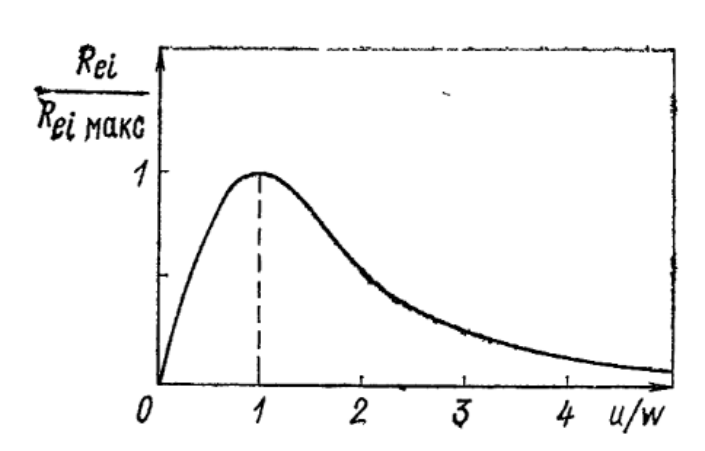
\includegraphics[width=70mm]{runaway_friction_force}
	\end{center}
	\caption{Общий вид зависимости силы трения электрон-ионных столкновений от средней скорости электрона [нормированную на тепловую скорость $\omega=v_T$]~\cite{golant}}
	\label{fig:runaway_el}
\end{figure}

При $\abs{eE}>R_\text{макс}$ сила трения не может уравновесить электрическую силу ни при каком значении направленной скорости. При
этом под действием электрического поля электроны перейдут в режим непрерывного ускорения. Критическая напряженность поля, определяющая границу такого перехода, равна $E_c\approx0.2\frac{eL_e}{\lambda_D^2}$ [критерий Дрейсера]. При ней электрон в среднем набирает энергию порядка тепловой.

Хотя критическое поле при типичных параметрах плазмы невелико, такое поле обычно трудно создать в полностью ионизованной плазме, обладающей высокой проводимостью. Однако и при меньших напряженностях поля возможно ``частичное убегание'' электронов, т. е. переход в режим ускорения быстрых электронов, для которых частота столкновений, определяющая трение, меньше, чем для основной массы.

Пусть у электрона скорость существенно большей тепловой ($v\gg v_T$). Сила трения, действующая на такой электрон, обусловлена их столкновениями с ионами и с основной массой электронов. Её нетрудно оценить, полагая, что относительная скорость при столкновениях примерно равна скорости искомой частицы:

\begin{equation*}
	R(v) = R_{ei}(v)+R_{ee}(v)\approx\mu_{ei}\nu_{ei}^t(v)v + \mu_{ee}\nu_{ee}^t(v)v \approx m_e\nu_{ei}^t(v)v + \frac{m_e}{2}4\nu_{ei}^t(v)v=\frac{12\pi n e^4}{m_ev^2}L_e,
\end{equation*}

Приравняв к электрической силе $eE$, найдём скорость, начиная с которой электроны переходят в режим ускорения:

\begin{equation*}
	\frac{m_eV^2}{T_e}>\frac{12\pi n e^3 L_e}{E T_e}\approx 15\frac{E_c}{E}
\end{equation*}

Таким образом, при $E<E_c$ основная масса электронов в электрическом поле движется с квазистационарной направленной скоростью, а в режим убегания попадают электроны из ``хвоста'' функции распределения. Со временем электроны приобретают все большую энергию и функция распределения ``вытягивается'' вдоль оси в направлении действия электрической силы. Такой процесс приводит к уменьшению функции распределения по сравнению с равновесной вблизи границы убегания. В результате возникает избыточный диффузионный поток электронов к границе убегания, вызванный в основном электрон-электронными соударениями, из области малых (тепловых) скоростей. Если бы не было препятствий неограниченному ускорению, то постепенно в режим убегания попали бы все электроны плазмы. Однако в реальных условиях существует ряд ограничений, препятствующих ускорению. Прежде всего время ускорения ограничено из-за ухода быстрых электронов из объема плазмы. Далее, в неполностью ионизованной плазме ускорение ограничивается столкновениями электронов с нейтральными частицами. При наличии сложных ионов возникает ограничение, связанное с тем, что потенциал иона на малом расстоянии существенно отличается от кулоновского и частота столкновений при больших скоростях перестает уменьшаться. Еще одной причиной, препятствующей ускорению, может быть излучение электронов при движении в плазме (т.н. ``радиационное трение''). Наконец, следует упомянуть о возможной раскачке кинетических неустойчивостей при прохождении быстрых электронов через плазму.

При учёте столкновений электронов с нейтральными частицами величина порогового поля меняется: $E_c^{(1)}$. При полях меньших $E_c^{(1)}$ стационарное распределение электронов по скоростям может быть близким к максвелловскому (равновесному). При $E_c^{(1)}<E<E_c$ имеется область скоростей, в пределах которой электроны увлекаются в режим ускорения. Эта область ограничена со стороны больших скоростей условием равенства электрической силы силе трения о нейтральные частицы: $m_e\nu_{ea}\vb{u}=e\vb{E}$. Вблизи границы области ускорения, при $\vb{v}\approx\vb{u}$, должно происходить накопление электронов, при этом должен образовываться максимум функции распределения, ширина которого зависит от соотношения между ускорением электронов в электрическом поле и диффузией в пространстве скоростей, обусловленной электрон-электронными столкновениями. При $E>E_c$, когда основная масса электронов переходит в режим ускорения, все распределение смещается в область скоростей, в которой электрическая сила уравновешивается трением электронов о нейтральный газ~\cite{golant}.

Есть ещё эффект \uline{убегания энергии} электронов. Рассмотрим сильноионизованную плазму в электрическом поле с основным механизмом потери энергии электронов в виде столкновений с ионами. Тогда можно оценить изменение электронной температуры в зависимости от электрического поля, исходя из баланса энергии: приравниваем  энергию $P_E$, приобретенную электронами в электрическом поле, к энергии $P_{ei}$, теряемой в столкновениях с ионами [$\beta_{ei}=const$]:

\begin{equation} \label{eq:runaway_el_balance}
	P_E = \sigma E^2 = 2\frac{ne^2 E^2}{m_e\nu_{ei}};\;P_{ei} = \frac{3}{2}\beta_{ei}n\nu_{ei}(T_e-T_i)
\end{equation}

Приравняем и оценим:

\begin{equation*}
	\frac{4}{3}\frac{e^2E^2}{m_e}=\beta_{ei}\nu_{ei}^2T_i\left(\frac{T_e}{T_i}-1\right) \sim \left(\frac{T_e}{T_i}\right)^3T_i(\frac{T_e}{T_i}-1)
\end{equation*}

Максимум у такой функции будет при $T_e=1.5T_i$. Постепенное увеличение напряженности поля $E$ от нуля до $E_c$ приводит к увеличению стационарной электронной температуры от $T_i$ до $1.5T_i$. При дальнейшем увеличении поля стационарное решение уравнения баланса энергий отсутствует. Это означает, что энергия, набираемая электронами в электрическом поле, превышает потери энергии при столкновениях и электронная температура нарастает со временем. Рост температуры приводит к дальнейшему падению частоты столкновений и нарастанию ``дизбаланса'' (режим убегания энергии).

В реальных условиях эффект убегания энергии ограничен другими механизмами потерь. В не полностью ионизованной плазме могут быть существенными потери, связанные со столкновениями электронов с нейтральными частицами. Другое существенное ограничение эффекта убегания энергии может быть связано с теплопроводностью плазмы, так как коэффициент теплопроводности быстро растет при увеличении электронной температуры $\varkappa_e\sim T_e^{5/2}$. Оценим, приравняв величину энергии, набираемой электронами в поле $P_E$, средним потерям энергии, связанным с теплопроводностью: $P_q = div(\varkappa_e\grad{T_e})\approx\varkappa_eT_e/L_T^2\sim nT_e^2/(m_e\nu_{ei}L_T^2)$, где $L_T$ -- масштаб неоднородности по $T_e$. В результате сравнения этого выражения с~\eqref{eq:runaway_el_balance} находим температуру в электрическом поле при условиях, когда теплопроводность является основным источником потерь:

\begin{equation*}
	T_{eq}\approx eEL_T
\end{equation*}

\subsection{Моменты функции распределения и переход к гидродинамическому описанию плазмы. Приближение квазигидродинамики, вывод диффузионных уравнений, явление термодиффузии и теплопроводности. Амбиполярная диффузия. ``Вмороженность'' магнитного поля в плазму. Нагрев электронов в постоянном и высокочастотном электрическом поле при наличии столкновений}

\subsubsection{Моменты функции распределения}

Да, в принципе кинетические уравнения позволяют найти функции распределения частиц и с их помощью определить макроскопические характеристики плазмы. Однако ввиду сложности кинетических уравнений получить их полное решение удается далеко не всегда. Многие задачи решаются с помощью приближенных уравнений для моментов функции распределения, которые можно получить из кинетических уравнений. Моменты функции распределения представляют собой комбинации компонент скорости частицы, усредненные по распределению, -- линейные (моменты первого порядка), квадратичные (моменты второго порядка) и пр.~\cite{golant}.

Рассмотрим ФР для частиц сорта $\alpha$ $f=f_\alpha(\vec{r}, \vec{v}, t)$~\eqref{eq:Boltzmann_eq}:

\begin{equation*}
	\pdv{f}{t}+(\vec{v}\nabla)f+\frac{q}{m}\left(\vec{E}+\left[\frac{\vec{v}}{c}, \vec{B}\right]\right)\pdv{f}{\vec{v}}=St\left\lbrace f\right\rbrace,
\end{equation*}

где заряд $q$ может быть равен $-e; +Ze; +e$.

[По сути, $n$-ый момент есть интегрирование функции распределения с весом $v^n$. Могут быть моменты и по координате, но здесь мы рассматриваем именно моменты по скорости]. \uline{$0^\text{ой}$ момент} -- концентрация/плотность частиц:

\begin{equation*}
	n(\vec{r}, t) = \int\limits_{\infty} f\dd[3]{v}
\end{equation*}

Пусть есть функция $u(\vec{v})$. Тогда \uline{$1^\text{ый}$ момент} [$\frac{1}{n}$ -- деление на норму; на самом деле есть три независимых первых момента -- три компоненты скорости, мы объединим три скалярных выражения в одно векторное]:

\begin{equation*}
	\left\langle u \right\rangle = \frac{1}{n}\int\limits_{\infty}uf\dd[3]{v}
\end{equation*}

Введём обозначение средней/направленной скорости: $\vec{u} = \left\langle \vec{v} \right\rangle$. Есть следующие ``вариации'' первого момента:

плотность тока $\vec{j} = q\int\limits_\infty\vec{v}f\dd[3]{v}=qn\vec{u}$; средний импульс $\vec{p} = m\int\limits_\infty\vec{v}f\dd[3]{v}=mn\vec{u}$; $\ldots$

Введём разность между полной и средней скоростью -- т.н. хаотическую скорость: $\vec{\omega}=\vec{v}-\vec{u}$. Тогда один из \uline{$2^\text{ых}$ моментов} -- объёмную плотность кинетической энергии -- можно выразить следующим образом:

\begin{equation*}
	K = \left\langle\frac{mv^2}{2}\right\rangle = \int\limits_\infty \frac{mv^2}{2}f\dd[3]{v} = \frac{mu^2}{2} + \frac{m\left\langle\omega^2\right\rangle }{2} = K_u + K_\omega = K_u + \frac{3}{2}T,
\end{equation*}

где температура $T$ вводится как мера средней энергии хаотического движения [если ФР -- максвелловская, то это можно легко показать]\Tokman. 

Моменты второго порядка, составленные из средних значений произведений произвольных компонент скорости, можно связать с потоком импульса. Компонента тензора плотности потока импульса, отвечающая за $k$-ую компоненту импульса, переносимого через единичную площадку в $l$-ой направлении\Tokman:

\begin{equation} \label{eq:momentum_flux_density_tensor}
	P_{jk} = mn\left\langle v_jv_k \right\rangle = mnu_ju_k+mn\left\langle \omega_j\omega_k\right\rangle,
\end{equation}

В системе отсчета, в которой средняя скорость $u=0$, этот тензор называется тензором давления $p$ [т.к. изменение импульса в единицу времени определяет приложенную силу]~\cite{golant}. Второе слагаемое представимо в виде

\begin{equation*}
	mn\left\langle \omega_j\omega_k\right\rangle = p_{jk} = p\delta_{jk}+\Pi_{jk};\;\Pi_{jk}\bigg|_{j=k} = 0
\end{equation*}

Недиагональные компоненты описывают силы, касательные к этим площадкам, и определяются видом ФР. Если ФР по хаотическим скоростям изотропна, то $\Pi_{jk} = 0$, а $p_{jk} = p = \frac{1}{3}nm\left\langle\omega^2\right\rangle=nT$. $\Pi$ называется \uline{тензором вязких напряжений} и равен:

\begin{equation*}
		\Pi_{jk} = nm\left\langle \omega_j\omega_k-\frac{1}{3}\omega\delta_{jk}\right\rangle 
\end{equation*}

Моменты третьего порядка составляются из средних значений произведений трех компонент скорости $\left\langle v_jv_kv_l\right\rangle $. Всего имеется десять независимых моментов этого типа. Наиболее важными из них являются моменты, связанные с потоком энергии~\cite{golant}:

\begin{equation} \label{eq:energy_flux}
	\vec{Q}=\int\limits_\infty\vec{v}\frac{mv^2}{2}f\dd[3]{v}=\frac{1}{2}mn\left\langle \vec{v}v^2\right\rangle = \vec{q} + nK_u\vec{u}+nK_\omega\vec{u}+P\vec{u},
\end{equation}

где $\vec{q}=\frac{nm}{2}\left\langle\vec{\omega}\omega^2 \right\rangle $ -- плотность потока тепла, отвечает за перенос энергии в с.о., где средняя скорость равна нулю и играет роль только хаотическое движение частиц; может быть малым. плотностью потока тепла. Остальные три слагаемых описывают поток, связанный с направленным движением, — перенос энергии самого направленного движения $\sim nK_u$, тепловой энергии $\sim nK_\omega$
и энергии, определяемой работой сил давления $\sim P$.

Уравнения на моменты ФР для описания движения заряженных частиц плазмы аналогичны гидродинамике, поэтому подобный подход называется гидродинамическим описанием плазмы. 

\subsubsection{Переход к гидродинамическому описанию плазмы. Приближение квазигидродинамики. Вывод диффузионных уравнений, явление термодиффузии и теплопроводности} \label{subsubsec:hydrodynamic_description}

Для получения уравнений на моменты ФР надо умножить кинетическое уравнение на комбинацию проекций скорости, соответствующую определенному моменту, и проинтегрировать его почленно по всему пространству скоростей. Умножая его на проекции скорости $v_k$, получаем уравнение первого момента, умножая на произведение $v_kv_l$ -- уравнение второго момента, умножая на $v_kv_lv_m$ -- уравнение третьего момента и т. д. Уравнением нулевого момента называют уравнение для концентрации, получающееся просто почленным интегрированием кинетического уравнения (уравнение непрерывности):

\begin{equation} \label{eq:continuity_eq}
	\pdv{n}{t}+div{\left(n \vec{v} \right)} = 0
\end{equation}

Уравнение первого момента (интегрируем~\eqref{eq:Boltzmann_eq}, пользуясь выражением~\eqref{eq:momentum_flux_density_tensor}):

\begin{equation*}
	\pdv{}{t}\left(nu_k\right) +\pdv{}{r_j}\left( nu_ju_k\right) +\pdv{r_j}P_{jk}-\frac{n}{m}qE_k-\frac{n}{m}q\left[\frac{\vec{u}}{c}\times\vec{B}\right]_k=\left[\int\limits_\infty \vec{v} St\left\lbrace f\right\rbrace\dd[3]{v}\right]_k
\end{equation*}

Интеграл от столкновительного члена берётся для случая полностью ионизованной плазмы или её пролёта через неподвижный газ (т.е. интеграл столкновений в форме Фоккера-Планка~\eqref{eq:Fokker-Planck_eq}):

\begin{equation*}
	\left[\int\limits_\infty \vec{v} St\left\lbrace f\right\rbrace \dd[3]{v} \right]_k = \int\limits_\infty A_kf\dd[3]{v}\xrightarrow{A_k = v_k\nu^t}nu_k\nu^{\text{eff}, t}
\end{equation*}

Тогда уравнение первого момента будет иметь следующий вид:

\begin{equation*}
	\pdv{}{t}\left(nu_k\right) +\pdv{}{r_j}\left( nu_ju_k\right) +\pdv{r_j}P_{jk}-\frac{n}{m}qE_k-\frac{n}{m}q\left[\frac{\vec{u}}{c}\times\vec{B}\right]_k=nu_k\nu^{\text{eff}, t}
\end{equation*}

Домножим на массу и перейдём к векторной форме [смогли вынести $n$ в левой части равенства за счёт использования уравнения непрерывности~\eqref{eq:continuity_eq}]:

\begin{equation*}
	nm\pdv{\vec{u}}{t}+nm(\vec{u}\cdot\nabla)\vec{u}= -\nabla P +qn\vec{E}+qn\left[\frac{\vec{u}}{c}\times\vec{B}\right]+mn\vec{u}\nu^{\text{eff}, t}
\end{equation*}

Проверка соблюдения физической логики: в силу закона сохранения импульса последний член обращается в нуль в случае столкновений между одинаковыми частицами. Кроме того, в таком виде он часто является хорошим приближением
для члена, описывающего трение. Дивергенция тензора давления
дает изменение импульса в единицу времени на единицу объема за счет пространственных неоднородностей. В этом члене учитывается влияние вязких сил~\cite{kroll}. 

Получили \uline{уравнение Эйлера} [из гидродинамики]. Для большего сходства можно ещё перейти от $P$ к $nT$, поделить на $nm$ и написать явный вид последнего слагаемого (напишем для электронов)\Tokman:

\begin{equation} \label{eq:Euler_eq}
	\pdv{\overrightarrow{u_e}}{t}+(\overrightarrow{u_e}\cdot\nabla)\overrightarrow{u_e} = -\frac{1}{n_em_e}\nabla P -\frac{e}{m_e}\left(\vec{E}+\left[\frac{\overrightarrow{u_e}}{c}\times\vec{B}\right]\right)-\nu_{ei}^{t}(\overrightarrow{u_e}-\overrightarrow{u_i})
\end{equation}

Для уравнения для ионов достаточно просто поменять индексы: $e\rightarrow i; i\rightarrow e$.

Рассмотрим уравнение второго момента (домножаем~\eqref{eq:Boltzmann_eq} на произведение двух компонент скорости и интегрируем). Учтём, что сила Лоренца работы не совершает и интеграл от неё будет равен 0. Получим уравнение баланса энергии:

\begin{equation*}
	\pdv{n\left\langle K\right\rangle}{t}+div\vec{Q}-qn\vec{E}\vec{u}=\int\limits_\infty\frac{mv^2}{2}St\left\lbrace f\right\rbrace \dd[3]{v}
\end{equation*}

Учтя~\eqref{eq:energy_flux}, получим:

\begin{equation*}
	n\pdv{}{t}\frac{mu^2}{2}+n(\vec{u}\cdot\nabla)\frac{mu^2}{2}-qn\vec{E}\vec{u}+\frac{3}{2}n\pdv{T}{t}+\frac{3}{2}n(\vec{u}\cdot\nabla)T+div(\vec{u}nT)+div\vec{q}+div(\vec{u}\Pi)=\int\limits_\infty\frac{mv^2}{2}St\left\lbrace f\right\rbrace \dd[3]{v}
\end{equation*}

Свернём первые два слагаемые и предположим, что тензор давления -- диагональный ($\Pi = 0$):

\begin{equation*}
	n\dv{}{t}\frac{mu^2}{2}-qn\vec{E}\vec{u}+\frac{3}{2}n\pdv{T}{t}+\frac{3}{2}n(\vec{u}\cdot\nabla)T+div(\vec{u}nT)+div\vec{q}=\int\limits_\infty\frac{mv^2}{2}St\left\lbrace f\right\rbrace \dd[3]{v}
\end{equation*}

Даже если интеграл от столкновительного члена есть функция только температуры, остаётся неопределённым $\vec{q}$. Можно идти разными путями: записывать уравнение третьего момента на величину $\vec{q}$ [в уравнении на $n$-ый момент входит величина, являющаяся переменной в уравнении на $n+1$-ый момент], либо замкнуть систему уравнений на этом шаге. Естественным шагом является предположение о том, что $\vec{q}=-\varkappa\nabla T$ (где $\varkappa$ -- \uline{теплопроводность}) -- для справедливости этого требуется какое-то знание о ФР (для квази-максвелловской -- работает\Tokman). Для модельного интеграла столкновений ($\tau$-приближение) это было посчитано ранее: см.~\eqref{subsec:transport_phenomena}.

Выбор того или иного способа обрыва цепочки макроскопических уравнений означает выбор определенной модели плазмы. Иногда используется изотермическое или адиабатическое уравнение состояния, а иногда хорошим предположением является р = 0~\cite{kroll}.

Получили три т.н. \uline{диффузионных уравнения}: на $n$, на $\vec{u}$, на $T$.

Условие применимости обрыва системы уравнений: столкновений должно быть много. Математически условие выглядит как $\lambda_{\alpha\beta}\ll L$, где $\lambda_{\alpha\beta}$ -- длина свободного пробега; $L \approx \frac{T}{T^{'}_x}$ -- характерный масштаб изменения температуры.

Существует два общих подхода к макроскопическому описанию плазмы. В первом электроны и ионы рассматриваются как две раздельно существующие, но взаимодействующие жидкости, каждая из которых описывается своей системой
уравнений и обладает определенными свойствами. В другом подходе плазма
описывается как одна жидкость со средней плотностью, скоростью и током
в каждой точке. Хотя оба эти подхода формально одинаковы, они нередко
связаны с различными приближениями~\cite{kroll}. Такое описание, СУДЯ ПО ВСЕМУ, и называется \uline{приближением квазигидродинамики}.

В подразделе~\ref{subsec:transport_phenomena} были рассмотрены простейшие случаи, когда имеется
либо только диффузионный, либо только тепловой поток, а
ФР была изотропной. В более сложных
случаях получатся и более сложные результаты. При одновременном протекании процессов диффузии и теплопередачи
диффузионный поток будет зависеть также и от градиента
температуры, а тепловой — также и от градиента концентрации. Эти явления носят название \uline{термодиффузии} и \uline{диффузионной теплопроводности}~\cite{frank}. Это можно аккуратно показать при использовании диффузионных уравнений.

\subsubsection{Амбиполярная диффузия}

Важнейшим фактором, влияющим на процессы переноса в плазме, является действие электрических полей. Поскольку ионы и электроны диффундируют с разной скоростью, то диффузия в плазме неизбежно приводит к разделению зарядов, а следовательно, и к возникновению электрических полей. Если разделение зарядов не снимается внешними проводниками, контактирующими с плазмой, то ионы и электроны не могут диффундировать независимо друг от друга. Возникающее электрическое поле вынуждает их к совместной, или \uline{амбиполярной диффузии}.

Рассмотрим диффузию заряженных частиц в слабо ионизованном газе~\cite{landau10}. Пренебрежём столкновениями между заряженными частицами по сравнению с соударениями с нейтральными. В процессе диффузии возникает электрическое поле. Уравнения диффузии тогда имеют вид:

\begin{equation*}
	\pdv{n_e}{t} + div\vb{i}_e = 0,\;\pdv{n_i}{t} + div\vb{i}_i = 0,
\end{equation*}

где плотности потоков равны:

\begin{equation*}
	\vb{i}_e = -n_eb_ee\vb{E}-D_e\grad{n_e},\;\vb{i}_i = n_ib_ie\vb{E}-D_i\grad{n_i},
\end{equation*}

где коэффициенты диффузии $D_e$, $D_i$ и подвижности электронов и ионов $b_e$, $b_i$ связаны соотношениями Эйнштейна (см.~\ref{par:diffusion}):

\begin{equation*}
	D_e = Tb_e,\;D_i = Tb_i
\end{equation*}

Вместе с уравнением Пуассона получаем систему уравнений:

\begin{align*}
	\pdv{n_e}{t} &= D_e div\left[\grad{n_e}-\frac{en_e}{T} \grad{\phi}\right]; \\
	\pdv{n_i}{t} &= D_i div\left[\grad{n_i}+\frac{en_i}{T} \grad{\phi}\right]; \\
	\Delta \phi &= -4\pi e(n_i-n_e).
\end{align*}

Пусть распределение концентраций почти однородны и $n_e\approx n_i\approx n_0$. Тогда перепишем систему уравнений:

\begin{align*}
	\pdv{n_e}{t} &= D_e\left[\Delta n_e-\frac{n_e-n_i}{\lambda_D^2}\right];\\
	\pdv{n_i}{t} &= D_i\left[\Delta n_i+\frac{n_e-n_i}{\lambda_D^2}\right],
\end{align*}

где $\lambda_D = \left(\frac{4\pi e^2 n_0}{T}\right)^{-1/2}$ -- дебаевский радиус. Учтём, что $D_e\gg D_i$ ввиду

\begin{equation*}
	\frac{D_e}{D_i}\sim\frac{v_{T_e}}{v_{T_i}}\sim\sqrt{\frac{M}{m}}
\end{equation*}

Рассмотрим эволюцию слабого возмущения концентраций с характерным размером $L\gg\lambda_D$. Тогда первые слагаемые справа меньше вторых и, вычитая одно уравнение из другого, получим:

\begin{align*}
	\pdv{}{t}(\delta n_e-\delta n_i) &= -\frac{D_e}{\lambda_D^2} (\delta n_e-\delta n_i) \\
	\delta n_e-\delta n_i &= (\delta n_e-\delta n_i)_0e^{-\frac{D_e}{\lambda_D^2}t}
\end{align*}

Получили, что за характерное время $\tau_{e_1} \sim \frac{\lambda_D^2}{D_e}$ разность $\delta n_e-\delta n_i$ станет малой, а газ -- квазинейтральным. Следующая стадия процесса состоит в эволюции ФР (электронов) к равновесной, т.е. занулению правой части уравнения для них:

\begin{equation*}
	\delta n_e-\delta n_i = \lambda_D^2\Delta n_e \approx \lambda_D^2\Delta n_i \sim \frac{\lambda_D^2}{L^2}\delta n_i
\end{equation*}

Это -- диффузионная стадия с характерным временем $\tau_{e_2}\sim \frac{L^2}{D_e}$. Окончательная релаксация происходит с установлением равновесности для ионов согласно [двойка возникла из-за равенств слагаемых в квадратных скобках]

\begin{equation*}
	\pdv{n_i}{t} = 2D_i\Delta n_i
\end{equation*}

Таким образом, в течение времени $\sim \tau_i$ электроны и ионы диффундируют вместе с удвоенным коэффициентом диффузии ионов (эффект \uline{амбиполярной диффузии}). Половина этого коэффициента связана с собственной диффузией ионов, половина -- с электрическим полем, создаваемым разбегающимися электронами.

\subsubsection{ ``Вмороженность'' магнитного поля в плазму}

См. раздел~\ref{subsec:Alfven_th}.

\subsubsection{Нагрев электронов в постоянном и высокочастотном электрическом поле при наличии столкновений}

Если поместить свободный электрон в поле волны, он будет испытывать осцилляции без набора энергии.

Добавим в рассмотрение столкновения. В уравнение на ускорение частицы тогда должна стоять $\delta$-функция, которая действовала на частицу каждое $t=t_\text{между столкновениями}$. Чтобы учесть это обстоятельство, включим в уравнение движения ``среднего'' электрона
эффективную скорость потери импульса (транспортную частоту). Уравнения движения запишутся в следующем виде~\cite{raizer}:

\begin{align*}
	\dot{\vb{r}} &= \vb{v};\\ 
	m\dot{\vb{v}} &= -e\vb{E}\sin\omega t - m\vb{v}\nu_{tr} \\
\end{align*}

Решение будет иметь вид:

\begin{align*}
	\vb{r} &= \frac{e\vb{E}}{m(\omega^2+\nu_{tr}^2)} \sin\omega t +\frac{\nu_{tr}}{\omega}\frac{e\vb{E}}{m(\omega^2+\nu_{tr}^2)} \cos\omega t; \\
	\vb{v} &= \frac{\omega e\vb{E}}{m(\omega^2+\nu_{tr}^2)}\cos \omega t -\frac{\nu_{tr} e\vb{E}}{m(\omega^2+\nu_{tr}^2)}\sin \omega t
\end{align*}

Будет осуществляться эффективная диссипация энергии поля, которая передаётся электронам от электромагнитной волны благодаря актам рассеяния электронов. Средняя работа над электроном может быть найдена:

\begin{equation*}
	\langle -eEv \rangle =-\frac{e^2E^2}{2m (\omega^2+\nu_{tr}^2)} \nu_{tr}
\end{equation*}

В промежутке между столкновениями электрон под действием электрической силы приобретает некую кинетическую энергию, в среднем порядка $\varepsilon_\text{колеб}$. Если за период между столкновениями электрон успевает совершить много колебаний, то это величина порядка энергии свободных колебаний. В акте упругого рассеяния атомом электрон резко меняет направление своего движения без изменения абсолютного значения скорости и энергии. После этого поле начинает раскачивать электрон в новом по отношению к скорости направлении, т. е. как бы заново сообщает ему энергию порядка $\varepsilon_\text{колеб}$. Таким образом, в каждом акте рассеяния порция энергии, в среднем приобретенной от поля с момента предыдущего столкновения, переходит в энергию поступательного, хаотического движения. Макроскопически -- работа поля затрачивается на преодоление силы трения, вызванной столкновениями электрона.

Часто вводят эффективное значение греющего поля, когда частота поля сравнима с частотой столкновений.

\begin{equation*}
	\vb{E}_{eff} = \vb{E} \sqrt{\frac{\nu_{tr}^2}{\omega^2+\nu_{tr}^2}}
\end{equation*}

Подобное выражение можно получить и из мнимой части $\varepsilon$, которая отвечает потерям/поглощению волны -- эта энергия и идёт на нагрев электронов:

\begin{equation*}
	\varepsilon=1-\frac{\omega_p^2} {\omega (\omega+i\nu_{tr})} = 1-\frac{\omega_p^2}{(\omega^2 + \nu_{tr}^2)}-i \frac{\omega_p^2 \nu^2_{tr}}{(\omega^2 + \nu_{tr}^2)}
\end{equation*}

Роль столкновений характеризуется соотношением между эффективной частотой $\nu_{tr}$ и круговой частотой поля $\omega$. В пределе $\nu_TR$ решения приближаются к формулам для свободных колебаний. Пусть рассматривается СВЧ-излучение частоты $f = 3$ ГГц, $\omega = 1.9\cdot10^{10}$ с$^{-1}$. При $p = 1$ Торр $\nu_{tr} \approx 3\cdot10^9$ с$^{-1} \ll \omega$. Порог СВЧ-пробоя при таком давлении $E_0 = 500$ В/см. Тогда без учёта столкновений амплитуда смещения электрона равна $a = \frac{eE_0}{m\omega^2} = 2.5\cdot10^{-3}$ см $\ll \lambda = 10$ см, т.е. поле в электромагнитной волне ``однородно''.

\section{Движение заряженных частиц в электрическом и магнитном полях}

Какой-то текст 4

\subsection{Релятивистские уравнения движения заряженных частиц в электромагнитном поле. Точные решения в однородных постоянных полях и в поле бегущей плоской волны}

\textbf{Постоянные однородные поля}

Сначала рассмотрим движение в постоянных полях. В таком случае удобно заметить, что существует всего две принципиально различные конфигурации. Это связанно с существованием двух инвариантов поля: $\vb{E}\cdot\vb{B}$ и $E^2 - B^2$. Один отдельный случай, когда оба эти инварианта равны нулю и соответствует скрещенным и равным электрическому и магнитному полям, является частным случаем движения в плоской волне, которое рассматривается ниже. Во всех остальных случаях, когда хотя бы один из инвариантов отличен от нуля, за счёт преобразования Лоренца можно перейти в такую систему отсчёта, где электрическое и магнитное поля будут параллельны (при этом выделенное направление будет соответствовать большему из полей). Решим в общем случае задачу о движении электрона в параллельных магнитном и электрическом полях. Для определённости пусть они направлены вдоль оси $z$. Запишем уравнения движения:
\begin{align*}
	& \dv{\gamma}{t} = -eE\frac{p_z}{m^2c^2\gamma} \\
	& \dv{p_z}{t} = -eE \\
	& \dv{p_x}{t} = \frac{eB}{mc}\frac{p_y}{\gamma} \\
	& \dv{p_y}{t} = -\frac{eB}{mc}\frac{p_x}{\gamma} \\
\end{align*}
Заметим, что первые два уравнения можно решать отдельно. Они описывают ускорение электрона вдоль электрического поля и имеют следующее решение:
\begin{align*}
	& p_z(t) = p_{z,0} - eEt \\
	& \gamma(t) = \sqrt{\gamma_0^2 - \frac{2eEp_{z,0}t}{m^2c^2} + \frac{e^2E^2t^2}{m^2c^2} }
\end{align*}
Для удобства введём $\tau = t - p_{z,0}/eE$ и $\gamma_{\perp,0}^2 = \gamma_0^2 - p_{z,0}^2/m^2c^2$. По сути переходим к отсчёту времени от момента, когда продольный импульс электрона был равен нулю и вся энергия была связана с вращательным движением $\gamma_{\perp,0}^2 = 1 + p_{\perp}^2/m^2c^2$. В новых переменных
\begin{equation*}
	\gamma(\tau) = \sqrt{\gamma_{\perp, 0}^2 + \frac{e^2E^2\tau^2}{m^2c^2} }
\end{equation*}
Для решения уравнений движения в плоскости, перпендикулярной полям, введём комплексную переменную $w = p_x + i p_y$ и сложим уравнения, умножив одно из них на мнимую единицу:
\begin{equation*}
	\dv{w}{t} = -i w \frac{eB}{mc\gamma}
\end{equation*}
Ищем решение этого уравнения в виде: $w = p_\perp\exp{-i\varphi}$
\begin{equation*}
	\dv{\varphi}{\tau} = \frac{eB}{mc\gamma(\tau)}
\end{equation*}
\begin{align*}
	&\varphi = \frac{B}{E}\int\limits_0^{t}\frac{\dd \left(eE\tau / mc\gamma_{\perp,0}\right)}{\sqrt{1 + \left( \frac{eE\tau}{mc\gamma_{\perp,0}} \right)^2}}\\
	&\varphi = \frac{B}{E}\text{arcsinh}\left( \frac{eEt}{mc\gamma_{\perp,0}} \right)\\
	&ct = \frac{\varepsilon_{\perp,0}}{eE}\sinh{\left( \frac{E}{B}\varphi \right)}
\end{align*}
где $\varepsilon_{\perp,0}=mc^2\gamma_{\perp,0}$. Теперь найдём траекторию электрона:
\begin{align*}
	&w = p_x + ip_y = m\gamma \dv{}{t}\left( x + iy \right) = m\gamma\dv{\varphi}{t}\dv{}{\varphi}\left( x + iy \right) = \frac{eB}{c}\dv{}{\varphi}\left( x + iy \right)\\
	&p_\perp e^{-i\varphi} = \frac{eB}{c}\dv{}{\varphi}\left( x + iy \right) \\
	&x = \frac{cp_\perp}{eB}\sin\varphi\\
	&y = \frac{cp_\perp}{eB}\cos\varphi\\
\end{align*}
В итоге нашли решение в параметрическом виде (величины зависят от $\varphi$, которое в свою очередь зависит от $t$). Движение вдоль оси $z$~---~равноускоренное, вращение в плоскости $xy$ происходит с сохранением импульса и уменьшением скорости (т.к. увеличивается энергия). При этом радиус вращения также остаётся постоянным. Конечный шаг~---~переход обратно в лабораторную систему отсчёта, в которой поля ориентированны произвольно. Этот шаг добавляет простой снос со скоростью системы отсчёта, в которой мы находили решение.

\vspace{5mm}
\textbf{Плоская волна}

Для решения задачи о движении электрона в плоской волне удобно воспользоваться гамильтоновым формализмом, а не напрямую решать уравнения движения. Для начала определимся, что такое плоское волна. Плоская волна~---~это конфигурация полей, которая задаётся векторным потенциалом $\vb{A}$, лежащим в плоскости $xy$, и зависящим только от комбинации $ct - x \equiv \xi$. В таком случае электрическое и магнитное поля перпендикулярны друг другу и равны по амплитуде. Сначала не будем делать предположений о явном виде $\vb{A}$.

Запишем энергию электрона:
\begin{equation*}
	\varepsilon = \sqrt{m^2c^4 + \vb{p}^2 c^2}
\end{equation*}
Данное выражение нельзя считать гамильтонианом, т.к. гамильтониан необходимо записывать в канонически сопряжённых переменных. В ЭМ поле сопряжённым к координате $\vb{r}$ является обобщённый импульс:
\begin{equation*}
	\vb{\Pi} = \vb{p} - \frac{q}{c}\vb{A}(\vb{r})
\end{equation*}
где $q$~---~заряд частицы. Будем решать задачу для электрона $q=-e$
\begin{equation*}
	\vb{\Pi} = \vb{p} + \frac{e}{c}\vb{A}(\vb{r})
\end{equation*}
Записанную в переменных $\vb{r}$, $\vb{\Pi}$ энергию можно приравнять гамильтониану:
\begin{equation*}
	H = \sqrt{m^2c^4 + \left( \vb{\Pi} - \frac{e}{c}\vb{A}(\xi) \right)^2 c^2}
\end{equation*}
Теперь запишем уравнения гамильтона:
\begin{align*}
    &\pdv{\Pi_y}{t} = -\pdv{H}{y} = 0 ,\\
    &\pdv{\Pi_z}{t} = -\pdv{H}{z} = 0 ,\\
    &\pdv{\Pi_x}{t} = \pdv{p_x}{t} = -\pdv{H}{x} = \pdv{H}{\xi} ,\\
    &\dv{\varepsilon}{t} = \pdv{H}{t} + \pdv{\vb{\Pi}}{t}\pdv{H}{\vb{\Pi}}+ \pdv{\vb{r}}{t}\pdv{H}{\vb{r}} = \pdv{H}{t} = c\pdv{H}{\xi}
\end{align*}
Из этих уравнений получаем важные интегралы движения
\begin{align*}
    p_y + \frac{e}{c}A_y = \text{const} ,\\
    p_z + \frac{e}{c}A_z = \text{const} ,\\
    cp_x - \varepsilon = \text{const}.
\end{align*}
Константы определяются начальными условиями:
\begin{align*}
    &p_y = p_{y, 0} + \frac{e}{c}\left( A_y(\xi_0) - A_y(\xi) \right)\equiv p_{y, 0} + \frac{e}{c}\Delta A_y ,\\
    &p_z = p_{z, 0} + \frac{e}{c}\left( A_z(\xi_0) - A_z(\xi) \right)\equiv p_{z, 0} + \frac{e}{c}\Delta A_z ,\\
    &p_x = p_{x, 0} + \frac{\varepsilon-\varepsilon_0}{c}
\end{align*}
Подставим эти выражения в определение энергии
\begin{equation*}
    \varepsilon^2 = m^2 c^4 + p_x^2c^2 + p_y^2c^2 + p_z^2c^2
\end{equation*}
После несложных вычислений получаем
\begin{equation*}
    \varepsilon = \varepsilon_0 - \frac{2ecp_{y,0}\Delta A_y - e^2\Delta A_y^2 + 2ecp_{z,0}\Delta A_z - e^2\Delta A_z^2}{2\left( \varepsilon_0 - cp_{x,0} \right)}
\end{equation*}
Это выражение нам необходимо для вычисления зависимости фазы $\xi$ от времени:
\begin{align*}
	&\dv{\xi}{t} = c - \dv{x}{t} = c - v_x = c - \frac{p_x}{m\gamma} \\
	&ct = \int\frac{\dd\xi}{1 - \frac{p_x}{mc\gamma}} = \int\frac{\varepsilon\dd\xi}{\varepsilon-cp_x} = \frac{\int\varepsilon\dd\xi}{\varepsilon_0-cp_{x,0}}\\
	&ct = \frac{\varepsilon_0\left( \xi-\xi_0 \right)}{ \varepsilon_0 - cp_{x,0}}-\frac{1}{2\left( \varepsilon_0 - cp_{x,0} \right)^2}\int\limits_{\xi_0}^{\xi}\left( 2ecp_{y,0}\Delta A_y - e^2\Delta A_y^2 + 2ecp_{z,0}\Delta A_z - e^2\Delta A_z^2 \right)\dd\xi'
\end{align*}

\vspace{5mm}
\textbf{Скрещенные постоянные поля}

Рассмотрим случай постоянных однороных скрещенных полей, чему соответствует вектор потенциал в виде:
\begin{align*}
	A_y = A\xi \\
	A_z = 0
\end{align*}
В таком случае электрическое поле направлено по оси $y$, магнитное~---~по оси $z$ и их амплитуда равна $A$. Для простоты предположим, что $p_0=0$ (это всегда можно сделать переходом в систему отсчёта электрона). В таком случае:
\begin{align*}
	&p_y = \frac{eA\xi}{c} \\
	&p_z = 0 \\
	&ct = \xi + \frac{e^2A^2}{2m^2c^4}\int\limits {\xi}^2\dd\xi \\
	&ct = \xi + \left( \frac{e A}{mc^2} \right)^2 \frac{\xi^3}{6}
\end{align*}
По сути мы решили задачу в параметрическом виде.
\begin{align*}
	& ct = \xi + \left( \frac{e A}{mc^2} \right)^2 \frac{\xi^3}{6} \\
	& \varepsilon = mc^2 + \left( \frac{e A}{mc^2} \right)^2\frac{\xi^2}{2} \\
	& p_x = \left( \frac{e A}{mc^2} \right)^2\frac{\xi^2}{2c} \\
	& p_y = \frac{eA\xi}{c} \\
	& p_z = 0 
\end{align*}
Отсюда видно, что в направлении $\vb{E}\times\vb{B} ,$ электрон быстрее набирает импульс, чем в направлении электрического поля.

\vspace{5mm}
\textbf{Линейно-поляризованная монохроматическая волна}

Теперь применим выражения для плоской линейно поляризованной монохроматической волны. В таком случае
\begin{align*}
	A_y = A\sin\left( \omega \xi \right) \\
	A_z = 0
\end{align*}
\begin{align*}
	&\varepsilon = \varepsilon_0 - \frac{2ecp_{y,0}A \left( \sin\xi_0 - \sin\xi \right) - e^2 A^2 \left( \sin\xi_0 - \sin\xi \right)^2}{2\left( \varepsilon_0 - cp_{x,0} \right)}\\
	&ct = \frac{\varepsilon_0\left( \xi-\xi_0 \right)}{ \varepsilon_0 - cp_{x,0}}-\frac{1}{2\left( \varepsilon_0 - cp_{x,0} \right)^2}\int\limits_{\xi_0}^{\xi}\left( 2ecp_{y,0}A \left( \sin\xi_0 - \sin\xi \right) - e^2 A^2 \left( \sin\xi_0 - \sin\xi \right)^2  \right)\dd\xi'
\end{align*}
\begin{align*}
	&ct = \frac{\varepsilon_0\Delta\xi}{ \varepsilon_0 - cp_{x,0}}-\frac{1}{2\left( \varepsilon_0 - cp_{x,0} \right)^2}\left[ 2ecp_{y,0}A\left( \Delta\xi\sin\xi_0 + \cos\xi - \cos\xi_0 \right) - \right. \\
	&\left. - e^2A^2\left( \Delta\xi\sin^2\xi_0 + 2\sin\xi_0 \left( \cos\xi - \cos\xi_0 \right) + \frac{1}{2}\left( \Delta\xi - \cos\xi\sin\xi + \cos\xi_0\sin\xi_0 \right) \right) \right]
\end{align*}
\begin{align*}
	&ct = \Delta\xi \frac{2\varepsilon_0\left( \varepsilon_0 - cp_{x,0} \right) - 2ecp_{y,0}A \sin\xi_0 + e^2A^2\left( \frac{1}{2} + \sin^2\xi_0  \right)}{2\left( \varepsilon_0 - cp_{x,0} \right)^2} + \dots
\end{align*}

В этом уравнении второе слагаемое (троеточие) ограничено, поэтому легко понять, что при больших временах $t$ данное равенство выполняется при больших значениях $\Delta\xi$ и вторым слагаемым можно пренебречь. В таком случае мы считаем, что электрон вышел на стационарную траекторию, которая представляет из себя восьмёрку в некоторой системе отсчёта. Для того, чтобы выяснить, с какой скоростью движется эта система отсчёта, вычислим средний за период волны импульс. Так как на больших временах мы можем считать, что фаза меняется линейно со временем, то всё усреднение сводится к занулению всех членов $\sin\xi$, $\cos\xi$ и приравниванию членов $\sin^2\xi$, $\cos^2\xi$ к величине $1/2$.
\begin{align*}
	&\langle p_y \rangle = p_{y,0} + \frac{eA}{c}\sin\xi_0 \\
	&\langle p_z \rangle = p_{z,0} \\
	&\langle p_x \rangle = p_{x,0} + \frac{e^2A^2\left( \frac{1}{2} + \sin^2\xi_0 \right) - 2ecp_{y,0}A\sin\xi_0}{2c\left( \varepsilon_0 - p_{x,0} \right)} \\
	&\langle \varepsilon \rangle = \varepsilon_0 + c\left( \langle p_x \rangle - p_{x,0} \right)
\end{align*}
Отсюда видно, что если электрон ``стартует'' не с нулевой фазы ($\xi_0 \neq 0$), то он дрейфует вдоль электрического поля. И вне зависимости от фазы электрон дрейфует в направлении вектора Пойнтинга. Характерным для движения электрона в плоской волне является то, что продольный импульс $p_x$ пропорционален $A^2$, а поперечный~---~$A$. Поэтому в релятивистски сильной волне $A>1$ большая часть энергии электрона сидит в движении вдоль вектора пойнтинга, тогда как в релятивистски слабой $A<1$~---~в колебательном движении.

\vspace{5mm}
\textbf{Циркулярно-поляризованная монохроматическая волна}

Повторим вычисления для циркулярно-поляризованной волны, которой соответствует следующий векторный потенциал:
\begin{align*}
	A_y = A\sin\left( \omega \xi \right) \\
	A_y = A\cos\left( \omega \xi \right)
\end{align*}
Во всех выражениях выше появляются дополнительные слагаемые, но принципиально ничего не меняется. Ожнако очевидно меняется траектория. В циркулярно-поляризованной волне она представляет собой винтовую линиию. При этом усреднённые по периоду характеристики не отличаются от случая линейной поляризации:
\begin{align*}
	&\langle p_\perp \rangle = \frac{eA}{c} \\
	&\langle p_x \rangle = \frac{1}{mc} \left( \frac{eA}{2c} \right)^2  \\
\end{align*}
При этом поперечный импульс вращается с частотой волны и сохраняет свой модуль.

\subsection{Движение заряженной частицы в магнитной ловушке, адиабатические инварианты, неоклассический перенос}

Какой-то текст 6

\subsection{Движение частицы в слабо неоднородном высокочастотном электромагнитном поле, высокочастотный потенциал, влияние внешнего магнитного поля}

Какой-то текст 7

\subsection{Движение электрона в пространственно периодическом электрическом поле. Квазиимпульс и зонный спектр электронов. Экранировка зарядов в кристалле в приближении случайных фаз}

Какой-то текст 8

\section{Волны в плазме}

Какой-то текст 9

\subsection{Феноменологическое описание электродинамики сред с временной и пространственной дисперсией. Плоские монохроматические волны, тензор диэлектрической проницаемости, 	соотношение Крамерса-Кронига. Распространение волновых пакетов, плотность энергии и потока энергии квазимонохроматических электромагнитных волн в среде с временной дисперсией, волны с отрицательной энергией}
\subsubsection{Волны с отрицательной энергией}

[Кадомцев, стр. 106]
Вообще, мы привыкли полагать, что энергия, которую переносит волна, она положительна и равна для волны с $k$ и $\omega_k $ величине $\varepsilon= \omega_k N$.
Но пусть у нас вся среда приходит в движение со скоростью $V_x=-v_0$. Тогда энергия волны будет $\varepsilon= (\omega_k-kv_0) N$. (например, волна звуковая, движение среды - сверхзвуковое)
Условие Черенковского излучения получаются тоже отсюда. $\omega_k -kv=0$.
Если у нас есть ещё и колебательные степени свободы с частотой $\omega_0$, то может происходить обмен энергии между волной и осциллятором при условии резонанса.$\omega-kv_0=\pm \omega_0$.
Однако, может возбуждаться не только основная мода колебаний, а n-ая гармоника $\Omega_a$, например
то будет $\omega-kv_0=\pm n \Omega_a$

\subsection{Тензор диэлектрической проницаемости в холодной магнитоактивной плазме. Электромагнитные и потенциальные волны в изотропной плазме с учетом теплового движения в рамках гидродинамического описания. Классификация волн в магнитоактивной плазме. Тензор диэлектрической проницаемости плазмы в рамках кинетического описания} \label{subsec:cold_magentic_plasma_waves}

\uline{Магнито-активная} плазма -- помещенная в ``могучее'' стороннее магнитное поле\Tokman. Частый случай: ионосфера, космос, токамаки, $\ldots$ Дело ещё в том, что даже в изотропной плазме возбуждаются сильные токи, появляется магнитное поле -- и надо рассматривать плазму с этой точки зрения.

Важная часть рассмотрения -- линеаризация. Вспомним уравнение Эйлера из МГД:~\eqref{eq:Euler_eq}:

\begin{equation*}
	\pdv{\vb{u}}{t}+(\vb{u}\cdot\nabla)\vb{u} = \frac{\vb{F}}{m} -\frac{1}{nm}\nabla(nT)-\nu(\vb{u})
\end{equation*}

Максимально упростим. Последнее слагаемое справа мало при $\omega\gg\nu$, где $\omega$ -- частота рассматриваемого процесса (колебания/волны). Чаще всего выполняется -- последнее слагаемое рассматривается по теории возмущения, а в линейном приближении можно его выкинуть. Второе слагаемое слева $\sim E^2$ -- тоже выкинем [обратный пример: может играть роль доплеровского сдвига]. Из уравнения непрерывности~\eqref{eq:continuity_eq} следует, что $\delta n \sim \frac{vN}{L\omega}$, где $N$ -- невозмущённая концентрация; а $v$ -- возмущённая скорость. Тогда второе слагаемое справа можно оценить как

\begin{equation*}
	\frac{1}{mn}\nabla(nT)\sim\frac{1}{Nm}\frac{1}{L}\frac{vNT}{L\omega}\sim\omega v\frac{T}{mL^2\omega^2}\sim\omega v\frac{v_T^2}{v_{ph}^2}
\end{equation*} 

Сравнивая с первым слагаемым слева, получаем, что условием выкидывания второго слагаемого справа будет $v_{ph}\gg v_T$. Тогда остаётся:

\begin{equation*}
	\dot{\vb{v}}=\frac{\vb{F}}{m}
\end{equation*}

При этом уравнения движения решаются как будто в однородном поле: $\vb{r}$ -- параметр. Также $j = q\vb{v}N$ -- линейный отклик [на самом деле здесь должна быть разница электронных и ионных скоростей]. Связь плотности тока и силы -- локальная (нет пространственной дисперсии в таком рассмотрении).

Итак,

\begin{equation*}
	\dot{\vb{v}}=q\frac{\vb{E}}{m}+\frac{q}{cm}[\vb{v}\times\vb{B}],
\end{equation*}

где $q=\pm (Z)e$; $m=\left\lbrace m_e, m_i\right\rbrace$; $\vb{E}\rightarrow\vb{E}e^{-i\omega t}$, опускаем предполагающееся обозначение реальной части, вводим циклотронную частоту $\vb{\omega}_B = \frac{q\vb{B}}{mc}$, где выбираем ось $z$ по $\vb{B}$. Получаем систему уравнений:

\begin{align*}
	-i\omega v_x-\omega_B v_y &= \frac{q}{m}E_x;\\
	-i\omega v_y +\omega_B v_x &= \frac{q}{m}E_y;\\
	v_z &= i\frac{q}{m}\frac{1}{\omega}E_z. 
\end{align*}

Вводя две круговые поляризации/нормальные координаты $x\pm iy$, получаем:

\begin{equation*}
	v_\pm = i\frac{q}{m}\frac{E_\pm}{\omega\pm\omega_B},
\end{equation*}

где нижний индекс соответствует знаку поляризации. На \uline{циклотронном резонансе} $\omega=\omega_B$ так решать, конечно, нельзя. Для электронов: $q<0$, $E_{+}$ даёт резонанс (крутится в ту же сторону).

Далее можно вывести тензор магнито-активной плазмы по следующей цепочке:

\begin{equation*}
	v_x,\,v_y\rightarrow\vb{j}\rightarrow\vb{p}=\frac{\vb{j}}{-i\omega}\rightarrow\vb{D}=\vb{E}+4\pi\vb{P}=\hat{\epsilon}\vb{E}
\end{equation*}

Тогда для электронов [учтен знак $q$] \uline{тензор диэлектрической проницаемости в холодной \linebreak магнитоактивной плазме} имеет вид:

\begin{equation*}
	\epsilon_{ij} =
	\begin{pmatrix}
		\epsilon & ig & 0 \\
		-ig & \epsilon & 0 \\
		0 & 0 & \epsilon_\parallel
	\end{pmatrix},
\end{equation*}

где $\epsilon = 1-\frac{\omega_{pe}^2}{\omega^2-\omega_{Be}^2}$; $g = \frac{\omega_{pe}^2\omega_{Be}} {\omega\left(\omega^2-\omega_{Be}^2\right)}$; $\epsilon_\parallel = 1-\frac{\omega_{pe}^2}{\omega^2}$ [как без магнитного поля; если $\omega_{Be}\rightarrow 0$, то $g\rightarrow 0,\,\epsilon\rightarrow\epsilon_\parallel$].

Учтём ионы: $\epsilon = 1-\frac{\omega_{pe}^2}{\omega^2-\omega_{Be}^2}-\frac{\omega_{pi}^2}{\omega^2-\omega_{Bi}^2}$; $g = \frac{\omega_{pe}^2\omega_{Be}} {\omega\left(\omega^2-\omega_{Be}^2\right)}-\frac{\omega_{pi}^2\omega_{Bi}} {\omega\left(\omega^2-\omega_{Bi}^2\right)}$; $\epsilon_\parallel = 1-\frac{\omega_{pe}^2}{\omega^2}-\frac{\omega_{pi}^2}{\omega^2}$.

Условия применимости: идеальность плазмы. Т.к. рассматриваем холодную плазму, положим $T = 0$. 

Поглощения нет: оператор эрмитов ($\epsilon_{ij} = \epsilon_{ji}^{*}$) [пока не добавили столкновения].

Если рассматриваются низкие частоты $\omega\ll\omega_{Bi}, \omega_{Be}$, то 

\begin{equation*}
	\epsilon_{ij} \approx
	\begin{pmatrix}
		\epsilon_i & 0 & 0 \\
		0 & \epsilon_i & 0 \\
		0 & 0 & \epsilon_\parallel
	\end{pmatrix},
\end{equation*}

где $g$ отвечает за дрейф. Из уравнений Максвелла следует:

\begin{equation*}
	\curl\vb{E} = -\frac{1}{c}\pdv{\vb{B}}{t};\; \curl\vb{B}=\frac{1}{c}\pdv{\vb{D}}{t}\;\Rightarrow\curl\curl\vb{E} = \frac{\omega^2}{c^2}\vb{D}
\end{equation*}

\begin{equation} \label{eq:dispersion_det_eq}
	det(k^2\delta_{ij}-k_ik_j-\frac{\omega^2}{c^2}\epsilon_{ij})=0
\end{equation}

Решение $E$ для~\eqref{eq:dispersion_det_eq} тогда есть нормальная волна.

Ранее было одно выделенное направление -- магнитного поля (по нему направили ось $z$). Теперь пусть у волнового вектора $k$ нет компоненты по $x$: $k_z = k\cdot\cos\theta,\,k_y = k\cdot\sin\theta$ ($\theta$ по смыслу есть угол между магнитным полем и волновым вектором). 

Тогда условие~\eqref{eq:dispersion_det_eq} можно переписать:

\begin{equation*}
	\begin{vmatrix}
		k^2-\frac{\omega^2}{c^2}\epsilon & -i\frac{\omega^2}{c^2}g & 0 \\
		i\frac{\omega^2}{c^2}g & k^2-k_y^2- \frac{\omega^2}{c^2}\epsilon & -k_yk_z \\
		0 & -k_yk_z & k^2-k_z^2- \frac{\omega^2}{c^2}\epsilon_\parallel
	\end{vmatrix}=0
\end{equation*}

или ($n^2=\frac{c^2 k^2}{\omega^2}$)

\begin{equation*}
	\begin{vmatrix}
		n^2-\epsilon & -ig & 0 \\
		ig & n^2\cos^2\theta-\epsilon & -n^2\cos\theta\sin\theta \\
		0 & -n^2\cos\theta\sin\theta & n^2\sin^2\theta-\epsilon_\parallel
	\end{vmatrix}=0
\end{equation*}

Решение: три волны -- одна плазменная и два решения биквадратного уравнения.

\begin{equation*}
	\frac{E_x}{E_y}=\frac{ig}{n^2-\epsilon};\;\frac{E_z}{E_y}=\frac{n^2\sin\theta\cos\theta}{n^2\sin^2\theta-\epsilon_\parallel}
\end{equation*}

Вводя обозначения $v=\frac{\omega_{pe}^2}{\omega^2}$, $u=\frac{\omega_{Be}^2}{\omega^2}$, дисперсионку можно записать следующим образом (\uline{формула Эпплтона-Хартри}):

\begin{equation} \label{eq:Appleton_Hartree_eq}
	n_{o,e}^2=1-\frac{2v(1-v)}{2(1-v)-u\sin^2\theta \pm \sqrt{u^2 \sin^4\theta+4u(1-v)^2 \cos^2\theta}}, 
\end{equation}

где индексы $o, e$ соответствуют обыкновенной и необыкновенной волнам. $n^2=n^2(\omega,\omega_{pe},\omega_{Be},\theta)$. 

Свойства:

\begin{itemize}
	\item $v\rightarrow 1\;(\omega\rightarrow\omega_{pe})$
	
	Обозначение: $v = 1 = v_0 = v_c$: ``cut-off'' (``отсечка'').
	
	\begin{equation*}
		n_{o_{0}}^2=0
	\end{equation*}
	
	\item $v=1\mp\sqrt{u}\;$
	
	\begin{multline*}
		n_{o,e}^2=1-\frac{2(1\mp\sqrt{u})(\pm\sqrt{u})}{2(\pm\sqrt{u})-u\sin^2\theta \pm \sqrt{u^2 \sin^4\theta+4u^2 \cos^2\theta}}=\\1-\frac{2(-u\pm\sqrt{u})}{2(\pm\sqrt{u})-u\left(\sin^2\theta\pm\sqrt{\sin^4\theta+4\cos^2\theta}\right)}= 1-\frac{2(\pm\sqrt{u}-u)} {2(\pm\sqrt{u})-u\left(\sin^2\theta\pm\sqrt{\sin^4\theta+4-4\sin^2\theta}\right)}=\\
		1-\frac{2(\pm\sqrt{u}-u)}{2(\pm\sqrt{u})-u\left(\sin^2\theta+2-\sin^2\theta\right)}=1
	\end{multline*}
	
	\item $v_\infty$ [знаменатель обращается в ноль]
	
	\begin{align*}
		2(1-v_\infty)-u\sin^2\theta \pm \sqrt{u^2 \sin^4\theta+4u(1-v_\infty)^2 \cos^2\theta}=0 \\
		4(1-v_\infty)^2+u^2\sin^4\theta-4u(1-v_\infty)\sin^2\theta = u^2 \sin^4\theta+4u(1-v_\infty)^2 \cos^2\theta \\
		1-v_\infty-u(1-\cos^2\theta) = u(1-v_\infty)\cos^2\theta \\
		1-v_\infty-u = -uv_\infty\cos^2\theta\\
		v_\infty = \frac{u-1}{u\cos^2\theta-1}
	\end{align*}

\end{itemize}

\begin{itemize}
	\item Распространение строго вдоль ($\theta = 0$) (см. рис.~\ref{fig:disp_eq_th_0_u_less_1} и рис.~\ref{fig:disp_eq_th_0_u_more_1})
	
	\begin{equation*}
		n_{o,e}^2=1-\frac{2v(1-v)}{2(1-v) \pm \sqrt{4u(1-v)^2}} = 1-\frac{v}{1\pm\sqrt{u}}, 
	\end{equation*}

	Есть резонанс на электронах для необыкновенной волны.

	Важно обратить внимание на то, что формула~\eqref{eq:Appleton_Hartree_eq} не дает полного решения дисперсионного уравнения, нужно ещё учесть $\varepsilon_{\parallel}=0$ (отмечено пунктиром на рисунках) [случай: без магнитного поля].

	\begin{figure}[ht]
		\begin{center}
			\begin{minipage}[h]{0.35\linewidth}
				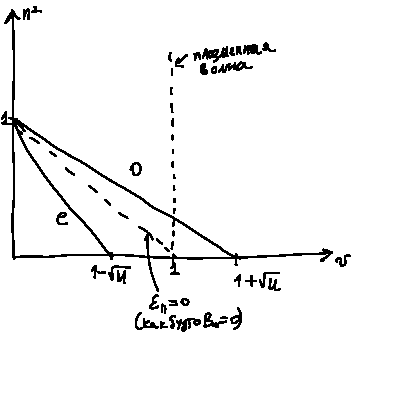
\includegraphics[width=1\linewidth]{theta0-u-less-1.pdf}
				\caption{Иллюстрация~\eqref{eq:Appleton_Hartree_eq} для $\theta=0, u<1$} 
				\label{fig:disp_eq_th_0_u_less_1}
			\end{minipage}
			\hfill
			\begin{minipage}[h]{0.35\linewidth}
				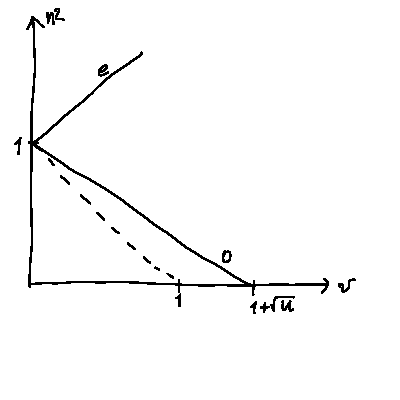
\includegraphics[width=1\linewidth]{theta0-u-more-1.pdf}
				\caption{Иллюстрация~\eqref{eq:Appleton_Hartree_eq} для $\theta=0, u>1$}
				\label{fig:disp_eq_th_0_u_more_1}
			\end{minipage}
		\end{center}
	\end{figure}
	
	\item Распространение почти вдоль ($\theta \ll 1$) (см. рис.~\ref{fig:disp_eq_th_small_u_less_1} и рис.~\ref{fig:disp_eq_th_small_u_more_1})

	Предельного перехода к случаю $\theta=0$ нет.
	
	Вблизи $v=1$ поляризация волн близка к продольной, т.е. к плазменной волне. Существование такой области называется \uline{эффектом Ландау-Зинера}.
	
	При наличии неоднородностей в областях сближения (две волны: частоты практически одинаковые, на масштабе биений поведение разное, на масштабах много больше длины волны -- одинаковое) одна волна может переходить в другую -- \uline{эффект линейного взаимодействия}. На самом деле подобное явление соответствует любому углу распространения, кроме строго поперёк -- его рассмотрим отдельно. Кроме того, к подобному эффекту могут приводить такие моменты, как учёт тепловых эффектов и др.

	\begin{figure}[ht]
		\begin{center}
			\begin{minipage}[h]{0.35\linewidth}
				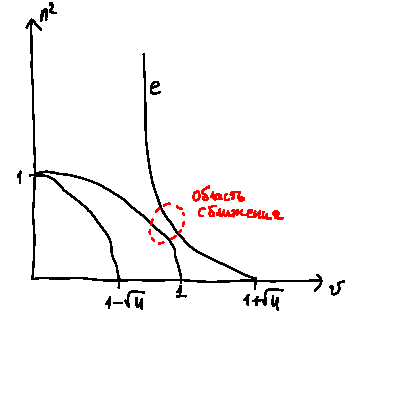
\includegraphics[width=1\linewidth]{theta-small-u-less-1.pdf}
				\caption{Иллюстрация~\eqref{eq:Appleton_Hartree_eq} для $\theta \ll 1, u<1$} 
				\label{fig:disp_eq_th_small_u_less_1}
			\end{minipage}
			\hfill
			\begin{minipage}[h]{0.35\linewidth}
				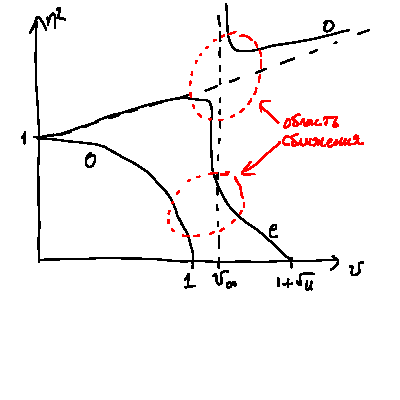
\includegraphics[width=1\linewidth]{theta-small-u-more-1.pdf}
				\caption{Иллюстрация~\eqref{eq:Appleton_Hartree_eq} для $\theta \ll 1, u>1$}
				\label{fig:disp_eq_th_small_u_more_1}
			\end{minipage}
		\end{center}
	\end{figure}

	\item Распространение поперёк ($\theta = \frac{\pi}{2}$) (см. рис.~\eqref{fig:disp_eq_pi_2})
	
	\begin{equation*}
		n_{o,e}^2=1-\frac{2v(1-v)}{2(1-v)-u \pm u}, 
	\end{equation*}

	\begin{equation*}
		n_o^2 = 1-v;\;n_e^2 = 1-\frac{v(1-v)}{1-v-u}
	\end{equation*}
	
	При учёте тепловых эффектов уже надо учитывать тепловую скорость, ведь $n^2\uparrow \Rightarrow v_{ph} \downarrow$, условие применимости теории может и не соблюдаться.
	
	При $u=1$ $n_o^2 = n_e^2 = 1-v$ обе волны крутятся по кругу против часовой стрелки -- т.е. в электронную сторону -- т.н. \uline{эффект депрессии циклотронного поглощения}.
	
	\begin{figure}[ht]
		\begin{center}
			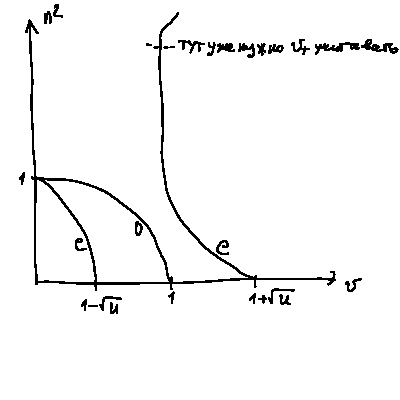
\includegraphics[width=0.35\linewidth]{theta-90.pdf}
		\end{center}
		\caption{Иллюстрация~\eqref{eq:Appleton_Hartree_eq} для $\theta=\pi/2$}		
		\label{fig:disp_eq_pi_2}
	\end{figure}
	
\end{itemize}

\subsubsection{Электромагнитные и потенциальные волны в изотропной плазме с учетом теплового движения в рамках гидродинамического описания. Классификация волн в магнитоактивной плазме}

\subsubsection{Тензор диэлектрической проницаемости плазмы в рамках кинетического описания}

Весь материал приводится по~\cite{akhiezer}.

Проблема предыдущего вывода: неучёт теплового движения частиц плазмы. Прежде всего благодаря тепловому движению ее частиц появляется ряд новых ветвей колебаний магнитоактивной плазмы, слабо- и сильнозатухающих, длинно- и коротковолновых, причем все они отсутствуют в холодной плазме (Напомним, что в отсутствие магнитного поля учет теплового движения электронов в плазме с холодными ионами и горячими электронами приводит к появлению только одной ветви колебаний: ионно-звуковых волн.).

Раньше: затухание Ландау -- результат взаимодействия резонансных частиц с электрическим полем волны, распространяющейся в плазме. Теперь, в магнитоактивной плазме: он же + циклотронный механизм затухания, связанный с излучением и поглощением электромагнитных волн заряженными частицами плазмы, движущимися в магнитном поле по спирали, на циклотронной и кратной ей частотах.

Случай высокотемпературной плазмы: большое время релаксации, квазиравновесное состояние, в котором ФР медленно изменяется из-за столкновений:

\begin{equation*}
	\frac{e_\alpha}{m_\alpha c}[\vb{v}\times\vb{B_0}]\pdv{f_{\alpha 0}}{\vb{v}}=-\omega_{B\alpha}\pdv{f_{\alpha 0}}{\theta} = 0
\end{equation*}

ФР тогда есть функция двух переменных: продольной и поперечной скоростей $v_\parallel$ и $v_\perp$ -- и не зависит от азимутального [$v_\parallel \parallel \vb{z};$  $\theta$ -- угол между $v_x$ и $v_\perp$] угла $\theta$.

Рассмотрим первый порядок теории возмущений. Считаем колебания высокочастотными, поэтому пренебрегаем интегралом столкновений. Запишем общий вид кинетического уравнения:

\begin{equation*}
	\pdv{F_\alpha}{t}+\vb{v}\pdv{F_\alpha}{\vb{r}}+\frac{e_\alpha}{m_\alpha}\left(\vb{E}+\frac{1}{c}[\vb{v}(\vb{B}+\vb{B_0})]\right)\pdv{F_\alpha}{\vb{v}}=0,
\end{equation*} 

где $F_\alpha = f_{\alpha 0}(v_\parallel, v_\perp)+f_\alpha(\vb{r},\vb{v},t)$. Линеаризуем:

\begin{equation*}
	\pdv{f_\alpha}{t}+\vb{v}\pdv{f_\alpha}{\vb{r}}+\frac{e_\alpha}{m_\alpha}\left(\vb{E}+\frac{1}{c}[\vb{v}\vb{B}]\right)\pdv{f_{\alpha 0}}{\vb{v}}-\omega_{B\alpha}\pdv{f_\alpha}{\theta}=0
\end{equation*}

Рассмотрим плоские монохроматические волны вида $exp[i(\vb{k}\vb{r}-\omega't)]$. Для них (с учётом $\vb{B}=\frac{c}{\omega'}[\vb{k}\vb{E}]$):

\begin{equation*}
	-i(\omega'-\vb{k}\vb{v})f_\alpha-\omega_{B\alpha}\pdv{f_\alpha}{\theta}=-\frac{e_\alpha}{m_\alpha}\left[\vb{E}\left(1-\frac{\vb{k}\vb{v}}{\omega'}\right)+\frac{\vb{v}(\vb{k}\vb{E})}{\omega'}\right]\pdv{f_{\alpha 0}}{\vb{v}} 
\end{equation*}

Далее в~\cite{akhiezer} приводится решение, разложенное по функциям Бесселя. В предположении, что эта информация выходит существенно за рамки кандидатского экзамена по физике плазмы, приведём ответ и некоторые свойства.

В случае слабозатухающих колебаний возмущение ФР $f_\alpha$ имеет резкий максимум при

\begin{equation*}
	v_\parallel = v_{\parallel,res}=\frac{\omega(\vb{k})-n\abs{\omega_{B\alpha}}}{k_\parallel},\;n=0,\pm1,\pm2,\ldots
\end{equation*}

Случай $n=0$: \uline{черенковский резонанс}. Иначе: циклотронный резонанс с учётом доплеровского смещения $k_\parallel v_\parallel$ [$n>0\Rightarrow v_{ph}>v_\parallel$ -- нормальный эффект Доплера, $n<0\Rightarrow v_{ph}<v_\parallel$ -- аномальный эффект Доплера].

В системе отсчёта, где $k_y=0$:

\begin{multline*}
	\epsilon_{ij} = \delta_{ij}+\sum\limits_{\alpha=e,i}\frac{4\pi e_\alpha}{m_\alpha\omega'^2}\biggl[\int\dd[3]{v}\left(\frac{\omega'-k_\parallel v_\parallel}{v_\perp}\pdv{f_{\alpha 0}}{v_\perp}+k_\parallel\pdv{f_{\alpha 0 }}{v_\parallel} \right)\frac{\Pi_{ij}^{(n)}(v)}{\omega'-k_\parallel v_\parallel -n\omega_{B\alpha}}- \\
	-b_ib_j\int\dd[3]{v}\left(f_{\alpha 0}+\frac{v_\parallel^2}{v_\perp}\pdv{f_{\alpha 0}}{v_\perp}\right)\biggl],
\end{multline*}

где

\begin{equation*}
	\Pi_{ij}^{(n)}(v) =
	\begin{pmatrix}
		\frac{n^2\omega_{B\alpha}^2}{k_x^2}J_n^2 & iv_\perp\frac{n\omega_{B\alpha}}{k_x}J_nJ_n' & v_\parallel\frac{n\omega_{B\alpha}}{k_x}J_n^2 \\
		-iv_\perp\frac{n\omega_{B\alpha}}{k_x}J_nJ_n' & v_\perp^2J_n'^2 & -iv_\parallel v_\perp J_nJ_n' \\
		v_\parallel\frac{n\omega_{B\alpha}}{k_x}J_n^2 & iv_\parallel v_\perp J_nJ_n' & v_\parallel^2J_n^2
	\end{pmatrix},
\end{equation*}

где $J_n = J_n(\lambda)$ и $J_n'$ -- функция Бесселя и её производные; $\lambda = k_xv_\perp/\omega_{B\alpha}$; $\vb{b}=\vb{B_0}/B_0$. Интегрирование производится аналогично~\ref{subsubsec:Landau_damping}.

Декремент затухания (или инкремент нарастания) волн определяется знаками величин $Im\epsilon_{ii}$, $Im\epsilon_{13}$, $Re\epsilon_{12}$, $Re\epsilon_{23}$, и которые в свою очередь зависят от знака величины

\begin{equation*}
	\left(k_\parallel\pdv{f_{\alpha 0}}{v_\parallel}+\frac{n\omega_{B\alpha}}{v_\perp}\pdv{f_{\alpha 0}}{v_\perp}\right)_{\omega=k_\parallel v_\parallel+n\omega_{B\alpha}} 
\end{equation*}

и от знаков функций Бесселя и их производных.

\subsection{Распространение электромагнитных волн в плоско-слоистой плазме. Нормальный и аномальный скин-эффект. Поглощение волн в областях плазменного и циклотронного резонанса. Линейная трансформация волн в изотропной плазме и магнитоактивной плазме, эффект предельной поляризации волн}

Какой-то текст 12

\subsection{Поверхностные волны на границе плазменного полупространства. Каналирование волн в плоских слоях с повышенной и пониженной плотностью плазмы. Резонансные характеристики простейших плазменных объектов – плоский слой, цилиндр, шар}

Какой-то текст 13

\subsection{Геометрооптическое описание волн в нестационарной плоскослоистой изотропной плазме. Геометрическая оптика в магнитоактивной плазме}

Какой-то текст 14

\section{Взаимодействие заряженных частиц с волнами в плазме}

Какой-то текст 15

\subsection{Понятие об абсолютной и конвективной неустойчивости. Кинетические и гидродинамические неустойчивости электромагнитных волн в плазме (примеры)}

\subsubsection{Абсолютная и конвективная неустойчивость.}
Абсолютная неустойчивость - явление при котором что-то нарастает в той точке пространства, где и начался спонтанный рост. КОнвективная - когда это возмущение ещё и двигается в какую-то сторону. См. рисунки. Так же из курса Гинзбурга можно вспомнить, что абсолютная неустойчивость реализуется при пересечении дисперсионок в случае, если они имеют разный знак групповых скоростей $\frac {d\omega}{dk}$. Конвективная, если в точке пересечения будут иметь одинаковый знак скоростей.
[картинки]
\subsubsection{Неустойчивости в плазме}
\label{subsec:plasma_B_instabilities}
[Кадомцев 212]
Гидромагнитные неустойчивости.
а) Желобковая неусточивость.
Рассмотрим одну из магнитных трубок ловушки. Пускай она отодвинется по радиусу относительно центра ловушки. При этом, объём её увеличивается. $V=\int s dl$ , где S - поперечное сечение трубки, а интеграл берётся вдоль силовой линии. Однако, у нас есть магнитный поток, который не должен меняться из-за вмороженности поля в плазму. $SB=\Phi$. Поэтому $V=\Phi \int \frac{dl}{B}$. И Трубка будет стремиться двигаться в направлении увеличения $U=\int \frac{dl}{B}$. По факту трубка будет иметь энергию $-pU$. И давление плазмы будет постоянным на поверхности одинакового $U$.
Относительно равновесия. Пусть её сдвиг происходит без искривления трубки, но с изменением объёма. То изменение объёма будет $\delta V/V= \delta U/U$, а изменение из-за адиабатического расширения $\delta p = -\gamma p \delta U/U$ 
Давление в окружающих трубках будет $p(U+\delta U)=p+(\frac{dp}{dU}) \delta U$
Тогда, если:
\begin{equation}
	-\gamma p \delta U/U > (\frac{dp}{dU}) \delta U
\end{equation}
Трубка будет пытаться уйти от центра. При другом же знаке, она будет наоборот стягиваться к центру, поэтому, условие устойчивости будет:
\begin{equation}
	\frac{ -\gamma p}{U} < \frac{dp}{dU}
\end{equation}
Рассмотрим с точки зрения магнитной гидродинамики это. На каждую компоненту (электроны и ионы), действует сила давления $nT_j /R$. Под её действием частицы начинают дрейфовать в азимутальном направлении.
Однако, на краях ловушки из неё вылетают частицы с слишком большими продольными скоростями, поэтому, давление плазмы продольное и поперечное не всегда равно. Поэтому, на плазме образуются желобки. Рассмотрим одну трубку в ней:
\begin{align*}
	m_i \frac{d v_x}{dt}= \frac{e}{c} v_{iy} B + \frac{T_i}{R}\\
	0= -\frac{e}{c} v_{x} B + \frac{T_i}{R}\\
	0= -\frac{e}{c} v_{ey} B + \frac{T_e}{R}
\end{align*}
Здесь принято, что в радиальном направлении плазменная трубка движется как целое. $v_{ix}=v_{ex}=v_x$. Электрическое поле $E$ возникает из-за поляризации трубки. Мы можем принять, что $E=- 4 \pi \sigma$, где $\sigma=en(\xi_{iy} - \xi_{ey})$. 

Тогда для электрического поля будет соотношение:
\begin{equation}
	\frac{\delta E}{\delta t} = -4 \pi e n (v_{iy}-v_{ey})=- \frac{d \pi c m_i n}{B} (\frac{d v_x}{dt} - g_0)
\end{equation}
, где $g_0=\frac{\omega^2_{pi}}{\omega^2_{pi}+\Omega^2_i}$ . При $\omega_{pi} <\Omega_{i}$ процесс выталкивания замедляется.

б) для борьбы с этим была сделана “магнитная яма”. Делают такую конфигурацию поля, чтобы оно всюду нарастало.

в) Винтовая неустойчивость. В желобковой неустойчивости, у нас высвобождалась только энергия плазмы, а магнитное поле в ловушке считалось фиксированным, что верно при $\beta \ll 1$ ($\beta=8 \pi p / B^2$). В винтовой раскачивает энергия магнитного поля.
Пусть есть проводящий электрический шнур из несжимаемой жидкости, который помещён в магнитное поле. Поле устроено в виде винта, то есть имеет и продольную $B_0$ и азимутальную. компоненту $B_{\theta} = 2I/cr$. Силовые линии являются винтовыми с шагом $l=2 \pi r B_0 / B_{\theta}$. На границе шнура этот шаг будет $l=l_a=\pi c a^2 B_0 /I$, а при удалении в радиальном направлении он возрастает как $r^2$.
Будем так же считать, что продольное $B_0$ много больше азимутального $B_{\theta}$. Так же, будем полагать, что шнур замкнут в виде тора, и длина шнура будет иметь длину $L=2\pi R$. И все возмущения имеют периодичность $L$. Пусть на такой шнур наложено некоторое малое винтовое возмущение вида $exp(im \theta + ikz)$, где $k=2 \pi n/L=n/R$, где $m,n$ - целые числа. Пусть $\xi$ - смещение жидкого элемента, так что $d[1]{\xi}{t}=v$. Тогда:
\begin{equation}
\frac{d^{2}\xi}{dt^{2}}= - \frac{1}{\rho_0} \grad p
\end{equation}
, где $\rho_0$ -  плотность жидкости, которая постоянно, $p$ - давление. В силу несжимаемости $div \xi =0$. От уравнения со 2-й производной берём градиент и получаем:
\begin{equation}
\Delta p = \frac{1}{r} \frac{d}{dr} (r \frac{dp}{dr})+(\frac{m^2}{r^2}+k^2)p=0
\end{equation}
Отсюда, при $kr \ll 1$ получаем $p=p_0 (r/a)^{m}$, где $p_0$ значение возмущённого давления на границе шнура, которое должно равняться возмущению давления магнитного поля снаружи от плазмы. Давление магнитного поля при этом:
\begin{equation}
\xi \frac{d}{dr}(\frac{B^2_0+B^2_{\theta}}{8 \pi}) + \frac{B B^{,}}{4 \pi}=p_0
\end{equation}
, где $B_0$ -возмущение магнитного поля, $\xi$ - радиальное смещение границы плазмы. Для колебаний вида $exp(-i \omega t)$ это смещение согласно формуле со второй производной по $\xi$ и с учётом, что $p \sim r^{m}$ равно:
\begin{equation}
\xi = \frac{1}{\rho_0 \omega^2} (\frac{dp}{dr})_{r=a-0}= \frac{p_0 m}{\rho_0 \omega^2 a}
\end{equation}

Подставляя возмущение магнитного поля и отклонение $\xi$ в уравнение на давление, можем получить дисперсионку:
\begin{equation}
4 \pi \rho_0 \omega^2=(kB_0 + \frac{m}{a} B_{\theta})^2 - \frac{m B^{2}_{theta}}{a^2}
\end{equation}
Отрицательным значениям квадрата частоты отвечает неустойчивость. Инкремент нарастания малых колебаний $\gamma = -i \omega$ достигает максимума при $ka=-mB_{theta}/B_0$. Такое возмущение является винтовым и имеет шаг $2 \pi m/k=2 \pi a B_0/B_{\theta}$ вдоль шнура. Шаг наиболее неустойчивой конфигурации совпадает с шагом винтовой линии. Вывод - надо чтобы отношение полей было иррациональным числом.
В этом случае $r$ трубки неустойчивости $r^2=a ln(b/a)$, где $a$ радиус шнура, $b$ - радиус кожуха.

Кинетические неусточивости.

а) неустойчивость пучка в плазме
У нас есть монохроматический электронный пучок в плазме с концентрацией $n_b$. Запишем дисперсионку для такой плазмы.
\begin{equation}
\varepsilon = 1-\frac{\omega^2_{pe}}{\omega^2}-\frac{n_b}{n} \frac{\omega^2_{pe}}{(\omega - kv)^2}
\end{equation}
Приравнивая $\varepsilon$ к 0, получаем инкремент неустойчивости (корень из отрицательной $\omega^2$). Когда $n_b \ll n$ Максимальный инкремент при $\omega_{pe}=kv$ равен $\gamma=(\frac{n_b}{2n})^{1/3}\omega_{pe}$.
Если пучок размыт по скоростям и имеется разброс в $\Delta V$ то при $\Delta V > \gamma/k$, мы можем оставить от пучка только мнимую часть вклада в $\varepsilon$. При этом дисперсионное уравнение принимает вид для холодной плазмы:
\begin{equation}
\varepsilon=1 - \frac{\omega^2_{pe}}{\omega^2} - \pi i \frac{\omega^2_{pe}}{n k^2} \frac{df}{dv}|_{v=\omega/k}=0
\end{equation}
Отсюда инкремент:
\begin{equation}
	 gamma=\frac{\pi\omega_{pe}}{2nk^2} \frac{df}{dv} |_{v=\omega_{pe}/k}
\end{equation}
б) ионный звук в плазме с током
Пускай $T_i \ll T_e$. Так же считаем, что функция распределения близка к максвелловской, но сдвинута на $u=-j/en$. Для нахождения инкремента воспользуемся выражением $\varepsilon=0$. Действительная часть для ионного звука была рассмотрена ранее, но тут интересна комплексная:
\begin{equation}
\varepsilon = 1 + \frac{\omega^2_{pi}}{k^2 c^2_s} - \frac{\omega^2_{pi}}{\omega^2} - \pi i \frac{\omega^2_{pi}}{nk^2} \int k \frac{\delta f}{\delta v} \delta (\omega - kv) dv =0
\end{equation}
Для сдвинутой Максвелловской функции распределения
\begin{equation}
\frac{\delta f}{\delta v} = - \frac{-m_e (v-u)}{T_e} f_e
\end{equation}
Инкремент в этом случае будет:
\begin{equation}
\gamma=\frac{\omega^3}{k^2 c^2_s} \sqrt{\frac{\pi m_e}{8T_e}} (u cos(\theta)- \frac{\omega}{k})
\end{equation}
, где $\theta$ - угол между $u k$. То есть ионно-звуковые волны начинают нарастать, когда скорость электронов превышает скорость ионного звука.
в) Кинетические конусные неустойчивости
Развиваются в закрытых ловушках. В таких ловушках нет частиц из конуса потерь, поэтому нету частиц с очень малыми поперечными скоростями, поэтому из 0 функция растёт. Также на бесконечности она убывает. Поэтому есть какой-то максимум в $v_0$. То есть, у нас тут инверсная заселённость по $v_{\perp}$. Поэтому, по аналогии с лазерами могут возникать волны, усиленные этими частицами.


\subsection{Эволюция функции распределения электронов в поле монохроматической плазменной волны. Квазилинейная теория, релаксация электронного пучка в плазме, ускорение частиц 	плазменной турбулентностью, механизм Ферми, формирование энергетического спектра частиц}
\subsubsection{Эволюция функции распределения электронов в поле монохроматической плазменной волны}
[Кадомцев, 2-е изд. стр. 186]
Пусть у нас летит плоская волна в плазме с какой-то функцией распределения. Введём их координату $\xi$ как отклонение от фронта волны с координатой “х”.
Уравнение тогда будет:
\begin{equation}
	\frac{d^2}{dt^{2}} \xi (x,t) = - \frac{e}{m_e} E(x+\xi,t)
\end{equation}
Эл поле определяется $E(x+\xi,t)=4 \pi e n_0 \xi$, тогда уравнение примет вид:
\begin{equation}
	\frac{d^2}{dt^{2}} \xi = - \omega^{2}_{pe} \xi
\end{equation}

\begin{figure}[ht]
	\begin{center}
		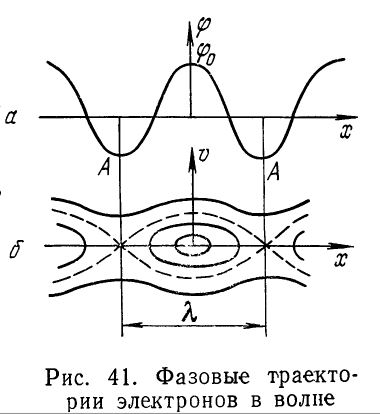
\includegraphics[width=70mm]{zatuh_landau_nonlinear_1.JPG}
	\end{center}
\end{figure}

То есть, видно, что электроны могут осциллировать в поле волны, которая летит через плазму. То есть в приближении холодной плазмы можно считать, что ленгмюровская волна имеет малую, но конечную амплитуду и её потенциал является гармонической функцией вида $\phi = \phi_0 cos(\omega_{pe} t -kx)$ .  Из-за теплового разброса будет происходить взаимодействие с резонансными частицами в плазме. Посмотрим, как будет двигаться электрон в таком потенциале. Перейдём в с.о. связанную с волной. Потенциал будет иметь вид $\phi = \phi_0 cos(kx)$. Ф.П. - кошачьи глаза. Есть 2 типа частиц в таком потенциале, пролётные (вне сепаратриссы) и захваченные (внутри сепаратриссы).
Сначала посмотрим, как электрон захваченный колеблется:
\begin{equation}
	m_e d^2 x=-eE=e \frac{\delta \phi}{\delta x}=-e \phi_0 k  sin(kx) \approx -e \phi_0 k^2 x
\end{equation}
Так что электрон будет совершать колебания с частотой $\Omega =k\sqrt{\frac{e \phi_0}{m_e}}$. По мере увеличения амплитуды колебаний электронов, частота уменьшается и на сепаратриссе обращается в 0. Определим сколько электронов (с какими скоростями) будут захваченными. Для этого посмотрим на ширину глаза в $x=0$. Тут у нас:
\begin{equation}
	\frac{m_e (v-v_{phase})^2}{2} - e \phi =const
\end{equation}
Ширина сепаратриссы в точке $x=0$ будет $\Delta v= 2 sqrt{e \phi_0 / m_e}$ , то есть она убывает с амплитудой волны гораздо медленнее, чем по линейному закону. 
Теперь посмотрим на функцию распределения. Для неё запишем уравнение Власова:
\begin{equation}
	\frac{\delta f}{\delta t} + v \frac{\delta f}{\delta x} + \frac{e}{m_e} \frac{\delta \phi}{\delta x} \frac{\delta f}{\delta v} =0 
\end{equation}
Так как скорость $v$ не зависит от координаты $x$, а ускорение от $v$, дифференциалы можно переставить и написать:
\begin{equation}
	\frac{\delta v}{\delta x} +\frac{\delta}{\delta v} (\frac{e}{m_e} \frac{\delta \phi}{\delta x} )=0
\end{equation}

\begin{figure}[ht]
	\begin{center}
		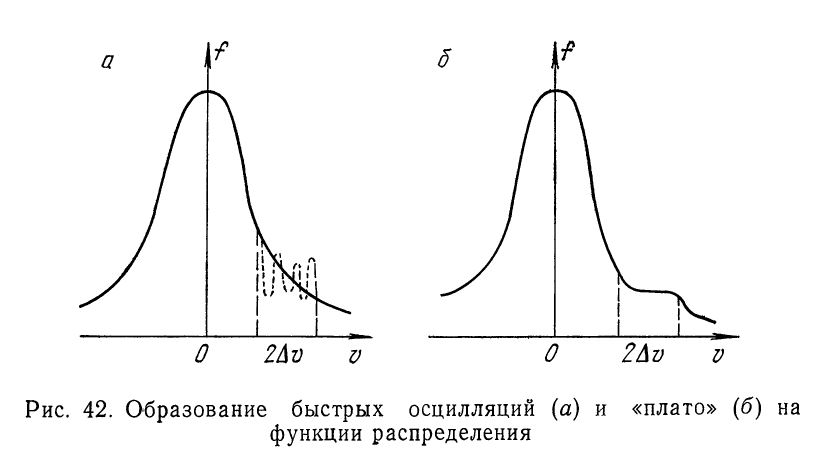
\includegraphics[width=70mm]{zatuh_landau_nonlinear_2.JPG}
	\end{center}
\end{figure}

\begin{figure}[ht]
	\begin{center}
		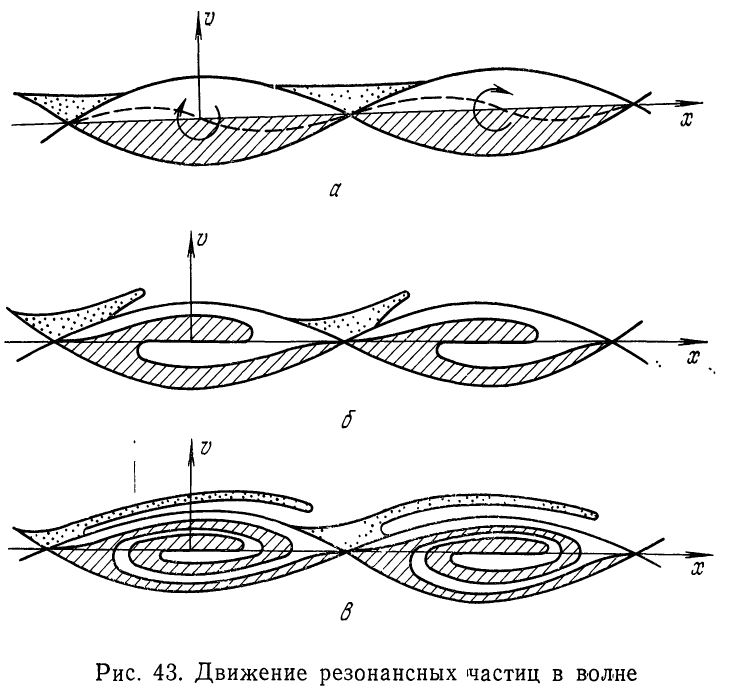
\includegraphics[width=70mm]{zatuh_landau_nonlinear_3.JPG}
	\end{center}
\end{figure}

Т.е. течение по f является несжимаемым. То есть f сохраняется вдоль линии тока. Поэтому, захваченные частицы с разбросом от $v_{phase} - \Delta v$ до  $v_{phase}+\Delta v$ будут иметь одну и ту же скорость, так как захваченные частицы быстро обмениваются энергией (из-за кулоновских столкновений, которые быстрее обычных столкновений).

Оценим амплитуду при которой можно считать волну нелинейной. Сравним плотность энергии в плоской волне:
\begin{equation}
	\varepsilon = \frac{E^{2}_0}{8 \pi} = \frac {k^2 \phi^{2}_0}{8 \pi}
\end{equation}
Энергия электронов в плато, ширина которого $\Delta v \sim \sqrt{e \phi_0 /m_e}$, а изменение энергии электрона при увеличении его скорости на $\Delta v$ вблизи фазовой скорости $\omega/k$ равно $m_e \Delta v \omega /k$ (по факту просто разложили $\frac{m(v+\Delta v)^2}{2}$).
Так как при образовании плато функция распределения меняется на величину:
\begin{equation}
	\Delta f \sim \frac{\delta f}{\delta v}|_{v=\omega/k} \Delta v
\end{equation}
Тогда изменение плотности энергии захваченных частиц по порядку величины равно:
\begin{equation}
	\Delta \varepsilon \sim m_e \frac{\omega}{k} \Delta v (\Delta f \Delta v ) \sim m_e (e \phi_0 /m_e)^{3/2} v \frac{\delta f}{\delta v}|_{v=\omega/k} 
\end{equation}
Вспоминаем, что у нас электроны имеют максвелловское распределение по скоростям, получаем:

\begin{equation}
	\sqrt{\frac{e \phi_0}{T_e}} \ll \frac{1}{(kd)^4} exp(-\frac{1}{2k^2 d^2})
\end{equation}

То есть при очень малых $kd$ даже оч малой амплитуды, может с собой много частиц уносить, и наоборот, при $kd > 1$ частиц будет мало


\subsection{Эхо в плазме. Аномальные диффузия, теплопроводность и сопротивление}

\subsubsection{Эхо в плазме.}
Самое первое эхо, которое обнаружили было спиновое эхо в экспериментах по ядерному резонансу. После двух импульсов с разницой в $\tau$ ответом от среды видели 3-й импульс, отстоящий на $\tau$.

\begin{figure}[ht]
	\begin{center}
		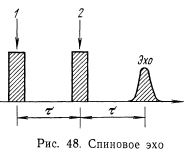
\includegraphics[width=70mm]{Echo_1_18.3.JPG}
	\end{center}
\end{figure}

Легче всего это увидеть на примере Циклотронного эха в плазме. Поперек столба созданной высокочастотным разрядом распадающейся плазмы, когда ток в ней практически отсутствовал и она была достаточно спокойной, пропускались два импульса высокочастотных колебаний с интервалом времени $\tau$. Плазма помещалась в магнитное поле около 3 кГс, а частота генератора была близка к циклотронной частоте электронов. Амплитуда импульсов была достаточно высокой, так что при циклотронном резонансе электроны могли приобретать энергию, значительно превышающую тепловую. После прохождения.
Что же происходило с точки зрения энергии электронов? Так как импульсы были довольно узкие, то из-за широкого спектра, он ВСЕ электроны приобретали одну и ту же энергию (скорость) (сдвиг на $v_p$ по диаграмме, рис. а.). После этого, электроны начинали вращаться с циклотронной частотой и скорость их стала не только по одной координате (из точки переросла в окружность с радиусом $v_p$). После того, как приходит второй импульс, то все электроны вновь смещаются на $v_p$ вдоль x (рис. в.). Эта смещённая окружность вновь должна расплыться по кругу вокруг (0;0) и будет иметь вид кривой на (рис. г.). 

\begin{figure}[ht]
	\begin{center}
		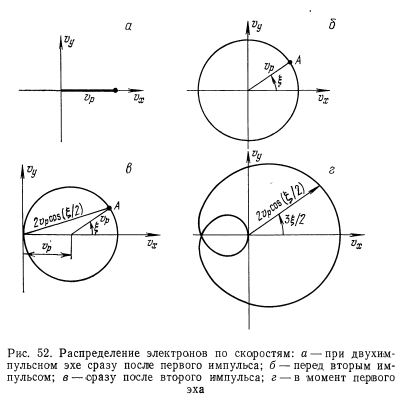
\includegraphics[width=70mm]{Echo_2_18.3.JPG}
	\end{center}
\end{figure}

Если будем следить за отдельными электронами, которые успели сдвинуться по фазе на $\xi$ в пространстве скоростей, то после второго импульса, они будут иметь скорость уже $2 v_p cos(\xi /2)$ и смещены на угол $\xi /2$ (см. рисунок). После времени $tau$ (за это время нужная пачка электронов повернулась на $\xi$) ВСЯ эта группа соберётся в точе отстающей по фазе на $3\xi/2 =\xi /2 + \xi $ .  А из рис. г. видно что может создавать эхо, но его не видно на картинке :D.
Чтобы циклотронное эхо проявилось, нужен нелинейный механизм. Это может быть релятивизим (масса от скорости) или зависимость частоты столкновений от скорости. Ну или трёхимпульсное эхо. 

\begin{figure}[ht]
	\begin{center}
		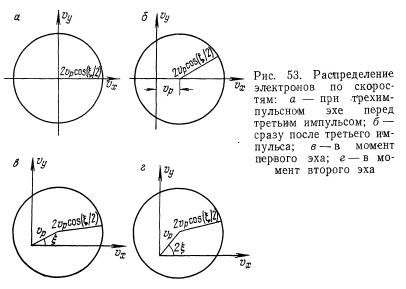
\includegraphics[width=70mm]{Echo_3_18.3.JPG}
	\end{center}
\end{figure}

Эхо может наблюдаться и на плазменных волнах.
На сетку, установленную в плазму подаётся сигнал с частотой значительно больше плазменной. Тогда и $\epsilon$ такой плазмы можно считать 1. В этом случае функцию распределения электронов можно представить как:
\begin{equation}
	f_1 (x,v,t)=f_1 (v) exp(-i \omega_1 t + i \omega_1 \frac{x}{v})
\end{equation}
, где  $f_1 (v)$ - амплитуда возмущения функции распределения вблизи сетки. Вид возмущения следует, что вдалеке это должно удовлетворять свободному движению частиц:
\begin{equation}
	\frac{\delta f_1}{\delta t} + v \frac{\delta f_1}{\delta x} =0
\end{equation}

Функцию распределения можно рассматривать как набор модулированных пучков, вблизи сетки они все по фазе колеблются, а по мере удаления - нет, поэтому плотность заряда
\begin{equation}
	\rho = -e \int f_1 dv
\end{equation}
должна быстро убывать при увеличении x.
ПУсть теперь на расстоянии d от сетки есть вторая, на которую подаётся переменный потенциал с частотой $\omega_2$ больше $\omega_{pe}$
Вторая сетка будет моделировать функцию $f_1$ так что появится нелинейный отклик $f_2$ на комбинационной частоте:
\begin{equation}
	f_2 (x,v,t)=f_2 (v) exp[-i \omega_1 (t-\frac{x}{v}) \pm i \omega_2 (t- \frac{x-d}{v})]
\end{equation}
При $x=d\frac{\omega_2}{\omega_2-\omega_1}$ экспонента, отвечающая частоте $\omega_2-\omega_1$ перестаёт зависеть от $v$. Это значит, что в точке
\begin{equation}
	x=d+d \frac{\omega_1}{\omega_2-\omega_1}=d  \frac{\omega_2}{\omega_2-\omega_1}
\end{equation}
должны наблюдаться заметные колебания плотности заряда на частоте $\omega^{,} = \omega_1-\omega_2 $ и зонд это может обнаружить.


\section{Нелинейные эффекты в плазме}

Какой-то текст 18

\subsection{Механизмы трехволнового взаимодействия в плазме. Примеры трехволновых процессов. Распадные неустойчивости. Соотношения Мэнли-Роу. Модифицированный распад. Процессы индуцированного рассеяния волн}
\label{subsec:3waveinterractive}

\subsubsection{Механизмы трехволнового взаимодействия в плазме. Примеры трехволновых процессов. Распадные неустойчивости. Соотношения Мэнли-Роу.}

Из уравнений Максвелла можно легко получить, что
\begin{equation}
	k^2 E - k (kE)+\frac{\omega^2}{c^2} D =0
\end{equation}
Но вот лучше добавить ток смещения (не самосогласованный ток) в правую часть
\begin{equation}
	k^2 E - \frac{c^2 k (kE)}{\omega}+\frac{\omega^2}{c^2} D =-\frac{4 \pi i \omega}{c^2} j_{s}
\end{equation}
так же сразу будем находить эл. поле как сумму по гармоникам
\begin{equation}
	E=\sum E_k exp(-i \omega_k t + ikr) + c.c.
\end{equation}
c.c. - комплексно сопряжённая часть.
Тогда для какой-то гармоники перепишется 

\begin{equation}
	\omega D_k - \frac{c^{2} k^{2}}{\omega} E_k + \frac{c^2 k(k E_k)}{\omega}=-4 \pi i j_{sk}
\end{equation}
Здесь $D=\hat{\epsilon} E$, вообще, у однородного этого уравнения имеются решения только совпадающих с собаственными частотами $\omega=\omega_k$. Да и чисто формально мы можем из D и $k^2-k(k e)$ по факту только перпендикулярная компонента можно сделать следующее:
\begin{equation}
	(\omega \epsilon - \frac{c^{2} k^{2}_{\perp}}{\omega}) E_k = -4 \pi i j_{sk}
\end{equation}
где $\epsilon=e^{*}_k \hat{\epsilon} e_k$, $k^{2}_{\perp}=k^{2}-|e_k k|^2$,$j_{sk}=e^{*}_k j_{sk}$
Вблизи $\omega=\omega_k$ левую часть вообще можно записать в виде множителя $A_k (\omega - \omega_k) E_k$.
\begin{equation}
	A_k=\frac{1}{\omega} \frac{\delta}{\delta \omega} (\omega^2 \epsilon) , \omega_k=\frac{ck_{\perp}}{\sqrt{\epsilon}}
\end{equation}
А для продольных волн с $k_{\perp}=0$ само $\epsilon$ обращается в 0 при   $\omega=\omega_k$ и величина $A_k= \omega \frac{\delta \epsilon}{\omega}$. То есть, уравнение перепишется:
\begin{equation}
	-i(\omega - \omega_k) E_k=-4 \pi i j_{sk}/A_k
\end{equation}
И действительно $E_k$ действительно велико вблизи $\omega=\omega_k$ и может даже расходиться в этой точке. Но это уравнение для фурье компоненты и фактически зависимость поля от времени:
\begin{equation}
	\int E_{\omega} exp(-i \omega t) d \omega
\end{equation}
Тогда $E_k (t) = \int E_{\omega} exp(-i \omega t) d \omega *exp(i \omega_k t)$ - это МЕДЛЕННАЯ амплитуда волны вблизи собственной частоты. То через фурье штуки получаем:
\begin{equation}
	\frac{\delta E_k}{\delta t} = \frac{4 \pi}{A_k} exp(i \omega_k t) j_{sk} (t)
\end{equation}
Тут $j_{sk} (t)$ сторонний ток как функция времени. То есть медленная амплитуда зависит от тока, который в свою очередь может зависеть от полей ВСЕХ гармоник. Вот тут и первый раз появляется нелинейность. Можно перейти к амплитудам волн и обезразмеренным операторам. То есть по факту:
\begin{equation}
	\frac{\delta a_k}{\delta t} =\sum_{k'} V_{k k^{,} k^{,,}} a_{^{,}} a_{k^{,,}} exp[-i(\omega_{k^{,}}+\omega_{k^{,,}}-\omega_k)] 
\end{equation}
Ну тут понятно, что из двух k’ и k’’ справа, должен получаться k, который слева, поэтому сразу ограничимся 3-мя волнами и запишем уравнения:
\begin{align}
	\frac{d a_1}{dt}=V1 a_2 a_3 \\
	\frac{d a_2}{dt}=V2 a_1 a^{*}_3 \\
	\frac{d a_3}{dt}=V3 a_1 a^{*}_2 \\
\end{align}
К.с. справа для того, чтобы выполнить $k_1=k_2+k_3'$ , $\omega_1=\omega_2+\omega_3$ . 
Умножим каждое уравнение на $\omega_i a^{*}_i$ и $k_i a^{*}_i$ и складывая их с к.с. получим законы сохранения энергии и импульса (соотношения Мейнли-Роу) 
\begin{align}
	\omega_1 |a_1|^2 + \omega_2 |a_2|^2 + \omega_3 |a_3|^2 = const \\
	k_1 |a_1|^2+ k_2 |a_2|^2 + k_3 |a_3|^2  = const \\	
\end{align}
Если взять какие-либо 2 уравнения и умножить их на недостающую комплексную амплитуду
\begin{align}
	\frac{d a_1}{dt} a^{*}_1=V1 a_2 a_3 a^{*}_1 \\
	\frac{d a_2}{dt} a^{*}_2=V2 a_1 a^{*}_3 a^{*}_2 \\
\end{align}
То ещё получится соотношение $a^{2}_1+a^{2}_2$.
Уравнение  $\omega_1 |a_1|^2 + \omega_2 |a_2|^2 + \omega_3 |a_3|^2 = const$ даёт нам поверхность эллипса в 3-х мерном пространстве,  $a^{2}_1+a^{2}_2$ - на поверхности этого эллипса выделит определённые линии, которые будут отвечать начальным условиям.

\begin{figure}[ht]
	\begin{center}
		\includegraphics[width=70mm]{Wavetrans1.JPG}
	\end{center}
\end{figure}

Тут есть 2 вида траекторий, которые отвечают устойчивым и неустойчивым состояниям.

\begin{figure}[ht]
	\begin{center}
		\includegraphics[width=70mm]{Wavetrans2.JPG}
	\end{center}
\end{figure}

\subsubsection{Модифицированный распад}
[М.В. Кузелов, Нелинейная теория излучения прямолинейным релятивистским пучком электронов в электростатическом поле накачки, ЖТФ, 1983, том 53, выпуск 6, 1029-1035]
Релятивистский пучок электронов, движущийся в периодическом поле, может быть источником когерентного коротковолнового излучения.
То есть, у нас есть волна периодического поля, есть “волна” электронного пучка, и они при сложении генерируют третью - волну рентгеновского излучения. 
При  модифицированном распаде механизмом насыщения неустойчивости является захват электронов комбинационной волной.(наблюдается при малой плотности электронов)




\subsection{Механизмы нелинейного самовоздействия волн в плазме (тепловые, силовые, ионизационные, релятивистские). Уравнения движения плазмы с учётом усреднённой силы со стороны высокочастотного поля. Модуляционная неустойчивость, ленгмюровские солитоны. Примеры самовоздействия электромагнитных волн в плазме (волноводные каналы, солитоны огибающих, ионизационное каналирование поверхностных волн)}

\label{subsec:nonlinearwaves}
\subsubsection{Механизмы нелинейного самовоздействия волн в плазме (тепловые, силовые, ионизационные, релятивистские)}
a) силовые - стрикционные


В общем случае $\varepsilon$ запишется как
\begin{align}
	\varepsilon=1-\frac{\omega^2_{pe}}{\omega^2} exp(-\frac{|\varepsilon^2|}{E^2_p})\\
	E^2_p=4(T_e + T_i) \frac{m \omega^2}{e^2}
\end{align}
В случае, когда $|\varepsilon| \ll E_p$:
\begin{equation}
	\varepsilon=\varepsilon_0 +\varepsilon^{,} |E|^2
\end{equation}
, где $\varepsilon_0=1-\frac{4 \pi e^2 N_0}{m \omega^2}=1-\frac{\omega^2_{pe}}{\omega^2}$, $\varepsilon^{,}=\frac{\omega^2_{pe}}{\omega^2 E^2_p}$ Среда с кубической нелинейностью. Мы уже знаем из параграфа \ref{subsubsec:Laitleh_crit}, что если у нас $\varepsilon$ зависит от $E$ то имеет место самофокусировка пакета.


б) тепловые


В этом случае:
\begin{equation}
	\varepsilon=\varepsilon_0 +\varepsilon^{,} |E|^2
\end{equation}
, где $\varepsilon^{,}=\frac{\omega^2_{pe}}{\omega^2 E^2_T}$.
Это значит, что $\varepsilon^{,}>0$, то есть диэлектрическая проницаемость в области поля растёт. $d \varepsilon/d|E|^2 >0$ (условно говоря, газ нагревается, давление падает, улучшаются условия пробоя и ещё лучше всё греется).


в) ионизационные


г) релятивитские
У нас обыкновенный:
\begin{equation}
	\varepsilon=1-\frac{4 \pi e^2 N}{m \omega^2}
\end{equation}
И в случае сверхсильных полей $m=m(|\vec E|)=m_0 + \delta m$, $\delta m \approx \frac{v^2}{c^2} m_0$
В линейно поляризованной волне: $\vec E= \vec y E(x)$
 \begin{equation}
 	\delta m= \frac{3}{4} \frac{e^2 E^2}{m^2 \omega^2 c^2} m_0
 \end{equation}
То есть в релятивизме тоже получили добавку к $\varepsilon_{\text{рел}}=\varepsilon_0 + \varepsilon^{,}_{rel} |E|^2$. Где $\varepsilon^{,}_{rel}=\frac{\omega^2_{pe}}{\omega^2 E_{rel}}$,$E^2_{rel}=\frac{4}{3}m^2c^2\omega^2/e^2$.


\subsection{Уравнения движения плазмы с учётом усреднённой силы со стороны ВЧ силы со стороны поля (сила Миллера)}
Про изменение локальной плотности плазмы будет написано ниже. ПРо уравнения движения - не знаю где брать.
\subsubsection{Модуляционная неустойчивость, Ленгмюровский солитон}
[Кадомцев, стр. 160]
Из уравнений мы знаем, что если есть $E=E_0 exp (i \phi)$ , то можно написать $\omega=\frac{d \phi}{dt}$, а $k=- \grad \phi$. Дифференцируя первое по $x$ второе по $t$ можно получить соотношение:
\begin{equation}
	\frac{\delta k}{\delta t} + v_{group} \frac{\delta k}{\delta x}=0
\end{equation}
Однако, если у нас не геом оптика, когда длина волны сравнима с неоднородностью в среде приходим к параболлическому выражению.
\begin{equation}
	i  \frac{\delta E}{\delta t} + i v_{group} \frac{\delta E}{\delta x} + \frac{v_{group}}{2 k_0} \Delta_{\perp} E + \frac{v^{,}_{group}}{2}  \frac{\delta^2 E}{\delta x^2}=0
\end{equation}
, где $v^{,}_{group}=\frac{\delta v_{group}}{\delta k}$ 
Когда волна распространяется по среде, у нас волновой пакет может расплываться, а бывают случаи, когда волновой пакет самосжимается.
Самый простой случай когда:
\begin{equation}
	\omega=\omega_k + \alpha a^2
\end{equation}
, где а - амплитуда волны. Подставим такое в наше уравнение:
\begin{equation}
	\frac{\delta k}{\delta t} = - \frac{\delta \omega}{\delta x}=-v_{group} \frac{\delta k}{\delta x} - \alpha \frac{\delta a^{2}}{\delta x}
\end{equation}
Также у нас есть условие сохранения энергии:
\begin{equation}
	\frac{\delta a^{2}}{\delta t} + \frac{\delta }{\delta x} (v_{group} a^2)=0 
\end{equation}
Из этих двух выражений видно, что плоская волна будет неусточива в некоторых случаях по отношению к разбиению на отдельные волновые пакеты. Пусть положим что:
\begin{align*}
	k=k_0 + k^{,} exp(-i \nu t + i \kappa x) \\
	a=a_0 + a^{,} exp(-i \nu t + i \kappa x) 
\end{align*}
Если инкремент малый, то $\nu=v_{group} \kappa \pm \kappa \sqrt{\alpha a^2_0 v^{,}_{group}}$, то есть при $\alpha v^{,}_{group} < 0$ имеем неустойчивость. (Критерий Лайтхила)
\label{subsubsec:Laitleh_crit}
Чтобы получить выражение для огибающей волнового пучка, то в параболлическое выражение подставим $E=exp(-i \nu_0 t) u(x-vt)$, то получим:
\begin{equation}
	\frac{\delta^2 u}{\delta x^2}=\frac{2 \alpha}{ v^{,}_{group}} u^{3} - \frac{2 \nu_0}{ v^{,}_{group}} u
\end{equation}
Теперь переходим к рассмотрению ленгмюровского солитона. В случае ленгмюровских волн имеем:
\begin{equation}
	\omega=\omega_{pe}+\frac{3T}{2 m_e \omega_{pe}} k^2
\end{equation}
Однако, оценим как волны могут возмущать плазму. А именно, что:
\begin{equation}
	\omega_{pe}=\omega_{p0}+ \frac{1}{2} \omega_{p0} \frac{\delta n}{n}+\frac{3T}{2 m_e \omega_{pe}} k^2
\end{equation}
, где $\omega_{p0}=\sqrt{4 \pi e^2 n/m_e}$ - невозмущённая ленгмюровская частота.
Но какое возмущение плотности плазмы может быть создано волной ?
Оказывается, плазма выталкивается силой Миллера. Если рассмотрим уравнение движения электрона в ВЧ поле:
\begin{equation}
	m_e \ddot x=-eE=-eE_0(x) cos(\omega t)
\end{equation}
Разбиваем $x=x_0 + \tilde x$ на две составляющие. Подставив в $E(x)=E(x_0 + \tilde x)=E(x_0)+ \tilde x \frac{dE}{dx} |_{x=x0}$.
Тогда у нас будет отдельно уравнение на быструю часть и на медленную.
\begin{align*}
	m_e \omega^2 \tilde x = -eE \\
	m_e \ddot x_0= - \langle e\frac{dE}{dx} \tilde x \rangle =- \frac{\partial }{\partial x} \frac{e^2 E^2}{4 m_e  \omega^2}
\end{align*}
То есть на электрон в среднем действует сила, создаваемая потенциалом $U=eE^2_0 /4m_e \omega^2=e \langle E^2 \rangle /2m_e \omega^2$. Зачастую, эта сила компенсируется давлением. 
\begin{equation}
	\frac{\partial}{\partial x} 2T \delta n = - \frac{\partial U}{\partial x}
\end{equation}
То есть
\begin{equation}
	\delta n= - \frac{e^2 E^2_0}{8 m_e  \omega^2_{p0} n T }=- \frac{3}{4} \frac{E^2_0}{8 \pi 3T}
\end{equation}
То есть $\delta n/n$ приблизительно равно отношению плотностей ВЧ и тепловой энергии. Теперь видно, что нелинейная добавка к частоте имеет вид $\alpha E^2_0$, где $\alpha= - \omega_{p0}/64 \pi n T$. То есть в ленгмюровских волнах тоже может быть эффект самосжатия.
Но нам надо знать $v^{,}_{group}$. Вспомним вид дисперсионки.
\begin{equation}
	\omega=\omega_{pe}+\frac{3T}{2 m_e \omega_{pe}} k^2
\end{equation}
Поэтому $v^{,}_{group}=\frac{v_{group}}{k_0}=3T/m_e \omega_{p0}$. Поэтому $2 \alpha / v^{,}_{group} = -e^2/24T^2$.
\begin{equation}
	\frac{\delta^2 u}{\delta x^2}=- \frac{2 \nu_0}{ v^{,}_{group}} u +\frac{2 \alpha}{ v^{,}_{group}} u^{3} 
\end{equation}

Это решение имеет решения типа солитона в виде $u=E_0/ch(x/\Delta)$. Тогда:
\begin{equation}
	\frac{\delta^2 u}{\delta x^2}= \frac{u}{\Delta} -\frac{2 u^{3}}{\Delta^2 E^2_0} 
\end{equation}
Тогда $\nu_0=-\frac{v_{group}}{2 \Delta^2}$ и $E^2_0 \Delta^2=-\frac{v^{,}_{group}}{\alpha}=\frac{48T^2}{e^2}$. То есть это будет огибающая с шириной $\Delta \sim 1/E_0$. Энеригия солитона $E^2_0 \Delta$ тем больше, чем больше амплитуда.
Фазовая скорость огибающей его волны $v_{phase}=\omega_{p0}/k_0$ может изменяться в широких пределах в зависимости от $k_0$. Для рассмотренного здесь солитона с равновесным распределением плотности величина $k_0$ ограничена сверху условием $v_{group}<c_{s}$, т.е. требованием, чтобы солитон был дозвуковым. Из этого вытекает условие что $k_0 d<\sqrt{m_e/m_i}$, где $d_0$ - дебаевская длина. 


\subsubsection{Примеры самовоздействия электромагнитных волн в плазме (волноводные каналы, солитоны огибающих, ионизационное каналирование поверхностных волн)}

\subsection{Сильная и слабая турбулентность плазмы. Параметрическое возбуждение ионно-звуковой и ленгмюровской волн в высокочастотном поле. Генерация “кавитонов” в области плазменного резонанса. Ионно-звуковые солитоны. МГД и бесстолкновительные ударные волны}

\subsubsection{Слабая турбулентность плазмы}
[Кадомцев, с. 251]
В плазме за счёт неустойчивостей возникают и затухают волны, которые в свою очередь тоже воздействуют на плазму. Вот пока мы несколько волн можем считать независимыми друг от друга, пока они не оказывают такого влияния на плазму, что изменяются её макропараметры. То такое взаимодействие называется слабой турбулентностью.
[Кингсеп]
Затухание или возбуждение волн сравнимо с феймановской диаграммой. Была частица с одним импульсом (одна функция распределения) она испустила квазичастицу (волну) и импульс изменился. Так вот пока мы эти квазичастицы считаем квазисвободными - это и есть приближение слабой турбулентнгсти.
[Кадомцев]
Пример слабой турбулентности - трёхволновое взаимодействие. Две волны приводят к нарастанию третьей. До каких пор она слабая ? До тех пор, пока энергия, колебаний, остаётся меньше тепловой энергии шумов. То есть:
\begin{equation}
\int \omega_k N_k dk = (T_i + T_e)n
\end{equation}
При этом $\frac{dN}{dt} \sim \omega N$. Поэтому по порядку величины $W \sim \omega^3/nT$, так что характерный масштаб темпа обмена энергией волн мб оценен как:
\begin{equation}
\frac{1}{\tau} \sim \frac{\omega \varepsilon}{nT}
\end{equation}
то есть приближение слабой турбулентностью применимо в случае $1/\omega T \sim \varepsilon/nT$
Индуцированное рассеяние волн на частицах - тоже турбулентнгость, так как там частица попадает в резонанс с биениями на комбинационных частицах и волновых векторах.
\begin{equation}
\omega_k \pm \omega_{k^{,}} - (k \pm k^{,})v=0
\end{equation}
Ионно-звуковая турбулентность
При протекании очень сильного электрического тока через разреженную плазму часто резко наблюдается увеличение её сопротивления, при чём оно сильно превышает сопротивление из-за кулоновских столкновений. Возникает из-за ударных волн поперёк магнитного поля.
Используется для быстрого введения в плазму джоулева тепла. Ток пускают вдоль магнитного поля, при этом очень быстро генерируются ионно-звуковые волны (см. неустойчисвоть ионного звука).
Условие неустойчивости: дрейфовая скорость электронов больше скорости звука:
\begin{equation}
\gamma \sim \omega \sqrt{\frac{m_e}{m_i}} (\frac{u}{c_s} cos(\theta) -1)
\end{equation}
Слабая ленгмюровская турбулентность
В разреженной плазме возникают такие условия, при которых происходит возбуждение ленгмюровских электронных колебаний. Такие волны могут возбуждаться эл.м. волнами, которые испытывают отражение от критической области, где плазменная частота совпадает с частотой излучения. Вблизи этой критической области эл.м. волна может трансформироваться в плазменную. Скорость передачи таких волн легко определить.
Максимальная скорость перекачки не может быть больше $\omega_pe$. Но также время должно определяться отношением энергии шумов к тепловой энергии $\varepsilon/kT$, так же существует экранирование волны электрон-ионной шубой. поэтому
\begin{equation}
\frac{1}{\tau} \sim \omega_{pe} (kd)^3 \frac{\varepsilon}{kT}
\end{equation}
Но рассеяние может быть и на ионах, тем более она играет большую роль в области больших волновых чисел. Для такого процесса
И как следствие скорость передачи:
\begin{equation}
\frac{1}{\tau} \sim \omega_{pe} (\frac{\Delta k}{k})^2 \frac{\varepsilon}{kT} \sim  \frac{\omega_{pe} m_e}{m_i (kd)^2}  \frac{\varepsilon}{kT}
\end{equation}
То есть при слабой турбулентности количество волн при рассеянии $N_k =const$ а энергия при этом. $\varepsilon_k = \omega_k N_k = [\omega_pe + \frac{3}{2} (kd)^2 \omega_{pe}]N_k$. То есть энергия ленгмюровских волн перекачивается в область с $k->0$ и приводит к образованию “конденсата” ленгмюровских колебаний.
\subsubsection{Сильная турбулентность плазмы}
Когда в области (этой областью является область плазменного резонанса) собирается слишком много квантов ленгмюровских колебаний (ленгмюровские сгустки), то они раскачивают продольные ленгмюровские волны, которые вытесняли плазму, создавая себе локальную яму [Кадомцев стр 266]. То есть, взаимодействие волн приводило к образовании “ямы” в концентрации плазмы.
Не обязательно “яма” должна быть именно в пространстве координат быть. Она может быть в пространстве скоростей. [Кингсеп]
\begin{figure}[ht]
	\begin{center}
		\includegraphics[width=70mm]{Turb_silnaya.JPG}
	\end{center}
\end{figure}


\subsubsection{Ионно-звуковые солитоны}
[Кадомцев, cтр. 262, спектр ионно-звуковой турбулентности, по факту, там где они $dN_k/dt$ к 0 приравняли]


\subsubsection{МГД и бесстолкновительные ударные волны}
[Кадомцев, МГД турбулентность, 270]
[Кадомцев, Эволюция бесстолкновительных систем,  277]


\section{Излучение плазмы}

Для описания излучения будем пользоваться т.н. квазиклассическим приближениемб условие применимости которого имеет вид:

\begin{equation}
    |\frac{d \lambda_{db}}{dx}|\ll 1,
\end{equation}
которое, для случая кулоновского потенциала $U=-Ze^2/r$, записывается в известном виде:

\begin{equation}
    \frac{Ze^2}{\hbar v} > 1,
\end{equation}
где $v$ - скорость электрона. Также стоит отметить, что для инфинитной траектории это условие имеет вид:

\begin{equation}
    \frac{m \rho v}{\hbar} \approx l \gg 1,
\end{equation}
где $l$ - квантовое число кол-ва движения.

Полезно также знать форулу для мощности дипольного излучения зарядом e:

\begin{equation}
    Q(t) = \frac{2e^2}{3c^3}|\ddot{\mathbf{r}}(t)|^2.
\end{equation}

Также вводят т.н. эффективное излучение: $\Delta \kappa = \int_0^{\inf} E(\rho) 2\pi \rho d\rho$, можно знаписать свять
спектральной мощности злучения ($\kappa$ в одну гармонику) с сечением:

\begin{equation}
    \frac{d\sigma}{d\omega}=\frac{1}{\hbar\omega} \frac{d\kappa}{d\omega}.
\end{equation}

\subsection{Виды излучения: Тормозное, магнитотормозное, черенковское, переходное, комптоновское. Нормальный и аномальный эффект Доплера. Особенности излучения релятивистских электронов. Синхротронное излучение в плазме. Сила реакции излучения; давление излучения в плазме}
Тормозное излучение представляет из себя свободно - свободый переход, возникает при инфинитном движении. 
Спектральное излучение в пределе больших частот($\omega \gg mv^3/Ze^2$) есть:

\begin{equation}
    \frac{d\kappa}{d\omega}=\frac{4\pi}{3}\frac{Z^2 e^6}{m^2 c^3 v_i^2}.
\end{equation}
В обратном случае излучение будет дипольным и вырадение принимает вид:

\begin{equation}
    \frac{d\kappa}{d\omega}=\frac{16}{3}\frac{Z^2 e^6}{m^2 c^3 v_i^2} \ln\left(\frac{2mv^3}{\delta \omega e^2 Z} \right),
\end{equation}
где $\delta \approx 1.78$.

Возможно также будут спрашивать про т.д.р. случай. Тут, следуя закону Кирхгофа, $\kappa$ зависит только от температуры среды. Спектральная мощность излучения из плазмы дается выражением:

\begin{equation}
    dQ(\omega)=N_i N_e \hbar \omega d\kappa(\omega).
\end{equation}

Когда электрон движется под углом к магнитному полю, он излучает т.н. магнитотормозное излучение(не важно есть среда или
нет, это общий термин). Если частица нерелятивистская, то излучение называется циклотронным (оно похоже на дипольное). В
случае, когда электрон реляливистский(ультрарелятивистский?) питч угол $\theta \gg mc^2/\varepsilon$, излучение
называется синхротронным. Когда имеет место обратное неравенство на питч угол, излучение носит название - релятивистское
дипольное, в этом случае можно перейти в с.о., где у элетрона скорость вдоль матнитого поля ноль и в этой системе
излучение будет циклотронным. В области релятивизма (умеренного?) $\varepsilon\gg mc^2$ излучение называется
гиросинхротронным.

Получим выражение для гармонк, воспользовавшись законами сохранения:

\begin{equation}
    \sqrt(m^2c^4+p_m^2c^2) - \sqrt(m^2c^4+p_n^2c^2)=\hbar \omega,
\end{equation}

\begin{equation}
    p_{|| m} - p_{|| n} = \frac{\hbar\omega}{c}n_j \cos(\alpha),
\end{equation}
где индексы $m$, $n$ соответствуют состояниям до и после испускания соответственно, $n_j$ - пок. преломления, $\alpha$ -
угол между волновым вектором и магнитным полем. Используя известное выражение для уровней Ладау можно записать вырадение
для изменение поперечной энергии:

\begin{equation}
    (p_{\perp m}^2 - p_{\perp n}^2)/2m = s\hbar\omega_B,
\end{equation}
где $s = 0, \pm1, \pm2, ..$ - номер гармоники.

Уравнение для гармоник можно найти в [Железняков, (10.28)] (оно большое и никто его не знает, так что...). Для слабо-
релятивистского электрона в вакууме решение (10.28):

\begin{equation}
    \omega = \frac{s\omega_B + \hbar \omega^2/2mc^2 \sin^2(\alpha)}{1-\beta_{||}\cos(\alpha)},
\end{equation}
второе слагаемое в числителе есть т.н. эффект отдачи - изменение частоты излучения за счет продольного импульса и
поперечной энергии.

\begin{equation}
    \omega = \frac{s\omega_B \sqrt(1-\beta^2)}{1-\beta_{||}\cos(\alpha)}.
\end{equation}
Случай $n_j\beta_{||}\cos(\alpha)<1$, называется нормальным эффектом Доплера, в данном случае излучение кванта
сопровождается переходом частицы и состояния с большей поперечной энергией в состояние с меньшей. Случай $n_j\beta_{||}\cos(\alpha)>1$,
назывется аномальным эффектом доплера - легко видеть, что при излучении поперечная энергия растет, энергия на то и на 
другое черпается из продольного движения. Легко видеть, что показатель преломления должен быть больше 1.
Из-за этого эффекта в анизотропных средах может происходить раскачка коллебаний осциллятора.

Циклотронное излучение(наверо надо пару слов). Тут следующие приближения: $\beta^2\ll1$, $|n_j\beta_{||}|\ll1$,
$|\beta_{||}\omega\frac{\partial n_j}{\partial \omega}|\ll1$, $|sn_j\beta_{\perp}\sin(\alpha)|$. Циклотронное 
излучение происходит только в области нормального эффекта Доплера. Частота циклотронного излучения $\omega=s\omega_B$,
на первой гармонике излучение дипольное, дальше мультиполные.

Синхротронное излучение.
Тут важно помнить выражения для потенциалов Линеара-Вихерта:

\begin{equation}
    \mathbf{A}=\frac{e\mathbf{v}}{c(R-\mathbf{R}\mathbf{v}/c)},
\end{equation}

\begin{equation}
    \phi=\frac{e}{c(R-\mathbf{R}\mathbf{v}/c)},
\end{equation}
величины в правой части берутся в запаздывающий мометн времени $t-R/c$. Знаменатель можно записать как:

\begin{equation}
    R - \mathbf{R}\mathbf{v}/c=R(1-\beta\cos(\theta))\approx R(1-\beta+\theta^2/2),
\end{equation}
откуда видно, что потенциалы велики в направлениях $\theta \ll 1/\gamma$. Излучение происходит преимущественно в
направлении движения частицы в конус с раствором $1/\gamma$. Рассмотрим вращение частицы в постоянном магнитном поле. 
Частица вращается по окружности с периодом $2\pi\gamma/\omega_B$. Тогда длительность импутьса в лабораторной системе:
$\Delta t = \frac{1}{\gamma^2\omega_B}$. Таким образом характерная частота, на которой происходит излучение есть 
$\omega_c \approx \gamma^2\omega_B$. Сам спектр очень широкий и имеет экспоненциальный хвост на больших частотах.

Пусть теперь есть среда, если $n>1$, то излучение направлено в черенковский конус(а не в направлении скорости, как в 
вакууме).
Существенные изменения в излучении будут, если $n<1$, и $1-n\ll1$. Подставляя $n$ в потенциалы ЛВ получим, что
ширина спектра определяется $\theta \approx \sqrt(1-n\beta)$. Если при этом $1-n^2\gg1/\gamma^2$, то ширина диаграммы
определяется полностью средой т.е. $\theta\approx\sqrt(1-n)$. Теперь потенциалы не стремятся к бесконечности, при
$\beta ->\inf$, происходит "депрессия" излучения.

Переходное излучение.
Суть(остатьное тут огромные формулы, их переписывать смысла нет): Пусть есть два диэлектрика $\varepsilon_1$,
$\varepsilon_2$, граница раздела находится в $z=0$. В области $z>0$ движется заряд $q$ в направлении $-z$. При переходе
через границу сред возникает переходное излчение.
Физика излучения следующая. Пусть заряд $q$ покоится (в точке x, y, d), тогда, как известно, для нахождения
полей в областях $z>0$ и $z<0$ используют метод изображений - помещают заряд
$q'=-q\frac{\varepsilon_1-\varepsilon_2}{\varepsilon_1+\varepsilon_2}$ 
слева(в области $z<0, \varepsilon_1$) в точке x,y,-d. В области $z>0$ помещают 
заряд $q''=q\frac{2\varepsilon_1}{\varepsilon_1+\varepsilon_2}$.
Когда заряд пересекает границу раздела, его изображения, какбы, резко меняют направление, т.е. меняется скорость
(точнее отношение скорости заряда к фазовой скорости излучаемой волны), и происходит излучение. Это похоже на то,
как возикает излучение, при движении заряда над гофрированной поверхностью проводника - в данном случае изображение 
осциллирует.

Сила реакции излучения.
Суть по простому - частица излучает, а значит теряет энергию. Эти потери можно представить в виде некой силы трения
(правда есть нюансы). Рассмотрим частицу двигающуюся по кругу. Потенциал ЛВ имеет следующий вид:

Комптоновское рассеяние.
Это рассеяние фотона на электроне, строгие выражения получаются из квантовой теории поля, но момжно получить
некторою информаци. используя законы сохранения. Запишем закон сохранения импульса и энергии:

\begin{equation}
    \mathbf{p}_e=\mathbf{p}_{\gamma}-\mathbf{p'}_{\gamma},
\end{equation}

\begin{equation}
    E_e + E_{\gamma}=E_e' +E_{\gamma}',
\end{equation}
выполняя простые переобразования, легко получить выражение для изменения длины волны:

\begin{equation}
    \lambda'-\lambda=\frac{\hbar}{2\pi mc} (1-\cos(\theta)),
\end{equation}
где угол $\theta$ есть угол между начальным и конечным импульсами фотона.

Давление в плазме (я ничего не нашел  в учебниках)
Давление эм волны определяется как:

\begin{equation}
    P = 2\frac{<S>}{c} = 2\frac{I}{c},
\end{equation}
где $I$ - интенсивность, или усредненный вектор пойнтинга. Можно записать вектор пойнтинга для среды с дисперсией:

\begin{equation}
    \mathbf{S}=\mathbf{S}_E-\frac{1}{16\pi}\frac{\partial}{\partial\mathbf{k}}(\varepsilon\omega)|E|^2-\frac{1}{16\pi}\frac{\partial}{\partial\mathbf{k}}(\mu\omega)|H|^2
\end{equation}


\begin{equation}
    \mathbf{A}=\frac{\mathbf{j}_0}{cr} \exp(ikr - i\omega t),
\end{equation}
запишем фурье компоненту для поля: 

\begin{equation}
    \mathbf{E}=ik_0\mathbf{A}+i/k_0 \grad div(\mathbf{A}),
\end{equation}
где $k_0=\omega/c$. После вычислений имеем:

\begin{equation}
    \mathbf{E}=\left( 
    \frac{ik_0\mathbf{r}\times[\mathbf{j}_0\times \mathbf{r}]}{cr^3} +
    \mathbf{j}_0\cdot\mathbf{r}\frac{3\mathbf{r}}{cr^4} - \mathbf{j}_0/(cr^2) +
    \frac{3i}{k_0c}\frac{\mathbf{j}_0\cdot\mathbf{r} \mathbf{r}}{r^5} - \frac{i\mathbf{j}_0}{k_0 cr^3}
              \right) \exp(ik_0r-i\omega t),
\end{equation}
видно, что есть 3 типа зависимости: $k_0/r, 1/r^2, 1/(k_0r^3)$. Рассмотрим поле около частицы (раскладываем экспоненту
по $k_0r$). Третье слагаемое в экспоненте даст в совокумности член, в котором нет особености в $r=0$, этот член 
имеет вид:

\begin{equation}
    \mathbf{E}_3=-\frac{2}{3}\frac{k_0^2}{c}\mathbf{j}_0\exp(-i\omega t) = \frac{2}{3c^3} \dddot{\mathbf{p}},
\end{equation}
Зная поле, можно записать силу, действующую на частицу и умножив на скорость и усреднив ее по периоду, получим

\begin{equation}
    P=<\mathbf{F}\mathbf{v}>=-\frac{2}{3c^3}|\ddot{\mathbf{p}}|^2,
\end{equation}
знакомая формула диполного излучения. Однаком мы говорим о силе: для нерелятивистского электрона можно записать уравнение

\begin{equation}
    m\dot{\mathbf{v}}=e\mathbf{E}+\frac{e}{c}[\mathbf{v}\times\mathbf{B}] + \frac{2e^2}{3c^3}\ddot{\mathbf{v}},
\end{equation}
это уравнение справедливо, когда сила трения много меньше силы Лоренца. Оно дает нефизичные решения (типа, когда
частица вылетает из области поля в свободное пр-во, но продолжает набирать скорость). Ограничение на силу можно
переписать $\lambda \gg e^2/mc^3$, т.е. мы не должны рассматривать процессы меньше некого радиуса. Это вообще 
довольно общие органичение на классическую электродинамику (его наверно лучше просто запомнить и не збивать голову
квантами).

\subsection{Тепловое и нетепловое излучения плазмы. Уравнение переноса излучения. Реабсорбция излучения, связь коэффициента поглощения и излучательной способности среды, метод коэффициентов Эйнштейна. Усиление излучения в неравновесной плазме. Вынужденное излучение из плазмы, в которой заданы начальные электронные токи}

Тепловое излучение есть эм излучение, генерируемое за счет энергии теплового движение частиц излучающего тела. Это
излчение удовлетворяет закону Кирхгофа - отношение излучающей способности, к его поглощающей зависит только от температуры
Излучение в основном генерируется электронами. Особенностью такого излучения является экспоненциальный спад
интенсивности на боьших частотах $I\sim \exp(-\hbar\omega/T)$.

Нетепловое - все остальное излучение, происходящее в неравновестных условиях.

Уравнение переноса излучения.
Явление переноса излучения с интенсивностью $I(\omega)$ характеризуется балансом процессов испускания и поглощения
квантов вдоль пути распространения излучения:

\begin{equation}
    \frac{dI(\omega)}{dx}=j(\omega)-\kappa(\omega)I(\omega),
\end{equation}
где $j$ - спонтанная излучательная способность, $\kappa$ - коэффициент поглоцения(с учетом индуцированного испускания).
Например, если есть атом с уровнями 1 и 0, и населеностями $N_0, N_1$, то:

\begin{equation}
    j(\omega)=N_1 A_{10}\hbar \omega G(\omega),
\end{equation}
где $A_{10}$ - коэффициент эйштейна спонтаного излучения, и $G$ - профиль линии излучения. Коэффициент поглощения:

\begin{equation}
    \kappa(\omega)=\hbar\omega (N_0 B_{01} - N_1 B_{10})G(\omega),
\end{equation}
где $B_{01}, B_{10}$ - коэффициенты эйнштейна для поглощения и индуцированного испускания. Связь коэффициентов:

\begin{equation}
    \frac{A_{10}}{B_{10}}=\frac{\hbar\omega_0^3}{\pi^2c^3},
\end{equation}

\begin{equation}
    \frac{B_{01}}{B_{10}}=\frac{g_1}{g_0},
\end{equation}
где $\omega_0$ - частота перехода между 1 и 0, $g_1, g_0$ - стат. веса уровней.

Если среда в тд равновесии, то следуя закону Кирхгофа:

\begin{equation}
    \frac{j}{\kappa}=\frac{\hbar\omega^3}{4\pi^3c^2}\frac{1}{\exp(\hbar\omega/T)-1}=B_{pl}.
\end{equation}

Оптическая толщина $d\tau=\kappa(\omega_0)dx$ - оптическая толщина среды. Обычно уравнение записывают так:

\begin{equation}
    \frac{dI(\omega)}{\tau}=-I(\omega) + S(\omega),
\end{equation}
где
\begin{equation}
    S(\omega) = \frac{N_1 A_{10}}{N_0 B_{01} - N_1 B_{10}}.
\end{equation}

Если среда в т.д. равновесии, и $N_1$ не зависит от координаты. Тогда можно найти интесивность:

\begin{equation}
    I(\omega) = B_{pi}\left( 1 - \exp(-L\frac{j}{B_{pl}})\right),
\end{equation}
откуда видно, что при большой толщине среды $L$ излучение определяется формулой плазмы. Если среда тонкая, то 
$I(\omega)\approx j(\omega)L$.

Усиление излучения в неравновесной плазме.

Уменьшение интенсивности на отрезке луча ед. длины (за счет переходов под действием излучения) равно:

\begin{equation}
    -\Delta I_\omega=\hbar\omega (N_n B_n^m - N_m B_m^n) I_\omega.
\end{equation}
Можно ввести коэффициент поглощения $\mu$:

\begin{equation}
    \mu=-\frac{\Delta I_\omega}{I_\omega}=\hbar\omega (N_n B_n^m - N_m B_m^n).
\end{equation}
В равновесной системе, используя формулы эйнштейна, можно записать:

\begin{equation}
    \mu=\frac{8\pi^3 c^2|\cos(\theta)}{n_j^2 \omega^2 T}a_\omega.
\end{equation}
Т.е. когда начеленности распределены по больцману, имеем, что и надо - зако Кирхгофа. Формулы выше записаны для переходов
между двумя состояниями только, иначе надо просуммировать по переходам между $m, n$.

\begin{equation}
    \mu=\frac{8\pi^3 c^2|\cos(\theta)}{n_j^2 \omega^2}\sum_{n<->m} A^n_m N_m (N_n/N_m - 1).
\end{equation}
Может случиться, что коэффициент реабсорбции $\mu$ будет отрицательным, т.е. будет усиление (это как лазер, только мазер).
Суть в том, что $\mu$ есть балас (разность) между интенсивностью поглощения и интенсивностью индуцированного испускания,
если последний процесс сильнее, то будет усиление. По сути, в данном случае имеется инверсия населенностей, как в
лазере. 
Этот коэффициент связан с декрементом следующим образом: $\gamma = \mu v_{gr}/2$, по этому в неравновесной плазме
может быть черенковская, синхротронная и циклотронная неустойчивости.

Черенковская неустойнивость это когда есть поток в плазме. Возникает эффект, обратный затуханию ландау - область, где
$\partial f/\partial v > 0$, по сути есть область инверсии населенностей. Поскольку: 

\begin{equation}
    N_m - N_n\approx \partial f/\partial v (\hbar k/m),
\end{equation}
где предполагалось, что ф.р. меняется слабо, при изменении импульса на $\hbar k/m$. Используя выражение для мощности
черенковского излучения можно записать выражения для реабсорции:

\begin{equation}
    \mu=-\frac{4\pi^2 e^2}{m\varepsilon} \int \partial f/\partial v \delta(\omega-kv) d^3v.
\end{equation}

\subsection{Рассеяние электромагнитных волн на флуктуациях плотности плазмы}

Какой-то текст 23b

\section{Специальные разделы физики плазмы}

\subsection{Инерционный управляемый термоядерный синтез, реакции термоядерного синтеза, критерий Лоусона, пороговая 
температура}
Идея инерционного утс заключасется в равномерном сжатии плазмы со всех сторон с помощью лазеров высокой энергии.
Перегретый поверхностный слой взрываясь наружу, создает реактивные силы действующие на мишень внутри, сжимая ее. Сжатие 
идет за счет ударных волн, направленных внутрь. Необходимо, чтобы серия таких ударных волн успела нагреть мишень, чтобы
начались термоядерные реакции. Обычно шарик топлива имеет размер булавочной головки, и содержит примерно 10 мг топлива.

Самые распространненные т.я. реакции (с самым большим сечением):
\begin{align}
    \prescript{1}{2}{D} + \prescript{1}{3}{T} \rightarrow \prescript{2}{4}{He} (3.52 MeV) + n (14.06 MeV),      \\
    \prescript{1}{2}{D} + \prescript{1}{2}{D} \rightarrow \prescript{1}{3}{T}  (1.01 MeV) + p (3.02 MeV), (50\%) \\
    \prescript{1}{2}{D} + \prescript{1}{2}{D} \rightarrow \prescript{2}{3}{He} (0.82 MeV) + n (2.45 MeV), (50\%) \\
    \prescript{1}{2}{D} + \prescript{2}{4}{He} \rightarrow \prescript{2}{4}{He} (3.6 MeV) + p (14.7 MeV),       \\
    \prescript{1}{3}{T} + \prescript{1}{3}{T} \rightarrow \prescript{2}{4}{He} + 2n + 11.3 MeV,                 \\
    \prescript{2}{3}{He} + \prescript{2}{3}{He} \rightarrow \prescript{2}{4}{He} + 2p + 12.9 MeV,
\end{align}

Критерий Лоунсона.
Позволяет оценить будет ли в реакторе положительный выход энергии за счет т.я. реакций. Чтобы это было так, необходимо,
чтобы кол-во выделяющегося тепла в данной реакции ($E_{r}*R*n^2$, где $E_r$- энергия в реакции, $R$ - скорость реакции) 
больше чем потери ($3/2 T * 2n / \tau$), и там и там $n$ - концентрация (считалась одинаковой для обоих участников реакции
, $\tau$ - время удержания плазмы. Результат зависит от реакции, для $D+T$ $n\tau > 2 10^{20}$, для $D+D$ $n\tau>5 10^{22}$.

Пороговая температура.




\subsection{Ускорение частиц. Ускорение на кильватерной волне и волне биений}
Необходимость новых методов ускорения связана в основном с громозкостью стандартных ускорителей (типа коллайдера и 
линейных ускорителей). Также теория показывает, что методами плазменного ускорения можно получать частицы с энергиями
плоть до $TeV$.

Кильватерная волна (пока в качестве драйвера будет лазер).
Электроны плазмы выводятся из равновесия (состояния невозмуженной плазмы) пондеромоторной силой лазера. Ионы можно считать
неподвижными на длинне лазерного импульса. Квазинейтральность нарушается и возникают области с сильным продольным 
электрическим полем, и эти колебания двигаются со скоростью драйвера. Это по сути и есть кильватерная волна. Если
честица попала в область этой волны, то она некоторое время будет ускоряться, причем до скоростей драйвера. 
В течении половины периода плазменной волны $T=2\pi c/\omega_p$ частица ускоряется, в течении второй половины - замедляется.
Максимальное поле, которое можно получить в волне можно оцеить из Пуассона, приняв в качестве температуры в вырадении для
радиуса дебая $T=mc^2$. Важно заметить, что в плазменной волне также есть и поперечные поля, т.е. на электрон будут
действовать поперечные силы. В линейном приближении поперечная вила есть $\sin(\omega t - kr)$. Половину своего периода 
эта сила - фокусирующая для электрона, другую половину - дефокусирующая. Однако, фаза поперечной силы сдвинута на $\pi/4$
поэтому только четверь периода плазменной волны идет ускорение электрона. 
Однако, из-за этого такая волна годится для ускорения позитронов (другая часть четверти периода фок. и уск. для них). В
нелинейном режиме (баббле) ускорять позитроны нельзя. Задняя половина баббла (там, где происходит захват) есть
ускоряющая область и передняя часть - замедляющая. Поперечные поля приводят к т.н. бетатронным колебаниям, которые либо 
фокусируют, либо дефокусируют частицу.

Если электрон попал в ускор. фазу, то его скорость может даже привысить скорость драйвера - он обгонит волну и выйдет из
уск. фазы. Длина дефазировки примерно как расстяние, которое пройдет электрон пересекая уск. и фок. области.

\begin{equation}
    l_{deph}\approx \frac{c\pi c/(2\omega_p)}{v - v_d} \sim \frac{\pi c}{\omega_p}\frac{\omega_l^2}{\omega_p^2}.
\end{equation}

Драйвер также тратит энергию на возбуждение плазменной волны. Для короткого импульса ($l < 2\pi c/\omega_p$) длина, 
характеризующая истощение лазера есть $l_{dp}\approx \frac{2\pi c}{\omega_p} \frac{\omega^2}{\omega_p^2}a_0^{-2}$.



\begin{figure}[ht]
	\begin{center}
		\includegraphics[width=0.6\linewidth]{wake-f.png}
	\end{center}
	\caption{Два вида кильватерных волн. Слева кильватерная волна в линейном режиме - по сути то, что образуется на 
    воде, при движении корабля. Справа - волна в нелинейном режиме, более известном как режим пузыря (за драйвером
    образуется полость практически без электронов).}
\end{figure}



\subsection{Магнитогидродинамика сильно разреженной плазмы в сильном магнитном поле. Гидродинамика Чу, Голдбергера, Лоу}

	В некоторых ситуациях (в астрофизике и газовом разряде) в физике плазмы часто возникают задачи, когда длина пробега электрона становится сравнимо больше любых других размеров системы. Частицы взаимодействуют друг с другом только с помощью дальнодействующих полей, которые описываются макроскопически. Всё равноценно тому, что все характерные влияющие размеры системы больше радиуса дебая. Тем самым, плазму мы уже не можем описывать как макроскопическую гидродинамическую систему, с такими г.д. параметрами как давление, плотность, масса скорость. Однако, было выдвинуто предположение, что сильное магнитное поле может служить источником рандомизации частиц и мы сможем описывать плазму в рамках гидродинамики.

Но эта попытка была не совсем удачная, это правда, что в какой-то степени можно ларморовский радиус считать за соударение электрона. Но эти «соударения» происходят только в поперечном направлении, в продольном – никаких столкновений не наблюдается. Поэтому нет никакой причины полагать, что чётные моменты функции распределения будут малы, что нужно для выполнения г.д. (написать условия применимости г.д.).

Поэтому для описания такой плазмы следует вновь стартовать с функции распределения. Как побочный продукт данного исследования мы можем показать, что электронная температура свободного движения электронов, может быть заменена макроскопическим током и на самом деле проблема окажется одножидкостной – ионной.
Бесстолкновительное уравнение больцмана для ионов принимает вид:
\begin{equation}
	\frac{\partial f}{\partial t}+(v grad)f+ \frac{e}{M}(E+v x B)grad_v  f=0 
\end{equation}
, где $f$- функция распределения, зависящая от $r,v,t$. Гауссова с.е., где $c=1$. 


Как и ранее хотим вычислить ф-ю распределения, однако уравнение трудное. Поэтому как и ранее, можем разложить по степеням малости $e/M$, что будет эквивалентно разложению по степеням Ларморовского радиуса ($r=\frac{MV}{eB}$). Эта процедура вообще может быть сравнима с адиабатической аппроксимацией, как только мы начали сравнивать Ларморовсвую частоту $eB/M$ с другими частотами в задаче.

Если разложим функцию распределения по степеням $M/e$:
\begin{equation}
	f=f_0 + f_1 +f_2+ ...
\end{equation}
Тогда уравнение больцмана разделится на серию уравнений:
\begin{align*}
	(E+v \times B) grad_v f_0 =0 \\
	(\frac{\partial }{\partial t} + v grad) f_0 + \frac{e}{M}(E+v \times B) grad_v f_1  =0 \\
	(\frac{\partial }{\partial t} + v grad) f_1 + \frac{e}{M}(E+v \times B) grad_v f_2  =0 \\
	e.t.c. .....
\end{align*}

И в общем, не очевидно, что она когда-либо замкнётся. Например, первое из системы не выполнится, пока эл. поле с магнитным не станут перпендикулярно. Однако, это условие как раз таки может быть выполнено, так как у нас в системе присуствтуют электроны. Из-за их малой массы и высокой подвижности любое эл. поле, направленное вдоль магнитных линий, приведёт к их движению и быстро перестанет существовать. Так же плазменная частота электрона($\omega_{pl} \sim \sqrt{ne^2/m}$), всё равно остаётся сильно больше Ларморовской частоты иона ($\omega_{L}=eB/M$), поэтому, так можно утверждать.

\begin{equation}
	\frac{\omega_{pl}}{\omega_{L}} \sim \sqrt{\frac{M nM}{m B^2}}
\end{equation}
Так как мы уже предположили, что электрическое и магнитное поле перпендикулярны, то можно ввести $\vec E=-\vec \alpha \times \vec B$. Так же вектор $\vec \alpha=\vec E \times \vec B /B^2$

Подставив это E в выражение для стационарной функции распределения, получим:

\begin{align*}
	(E+ v \times B) grad_v f_0 =0 	 \\
	(- \vec \alpha B + \vec v \times \vec B) grad_v f_0 =0 \\
	(\vec V \times \vec B) grad_v f_0 =0
\end{align*}
, где $V=v-\alpha$. Решение этого уравнения достаточно простое. Да, оно будет зависеть от $\vec V,\vec B$ , но не изменяться вдоль направления $\vec V \times \vec B$ 

Поэтому, самое общее решение будет $f_0 [(v-\alpha)^2,v,B,r,t]$
Глядя на это выражение, направление $\vec \alpha$ будет направлением средней скорости ионов, перпендикулярной B. Более того, $\vec \alpha$ будет и электронной средней скоростью, перпендикулярной B.

Проинтегрируем выражение для возмущённой ф-и распределения по всем V. Получим, уравнение гидродинамики.
\begin{align*}
	(\frac{\partial }{\partial t} + v grad) f_0 + \frac{e}{M}(E+v \times B) grad_v f_1  =0 \\
	\frac{\partial n_0}{\partial t} + div(n_0 f_0)  =0 \\
	n_0 = \int dv f_0 \\
	n_0  u_0=\int dv v f_0
\end{align*}


Можно сделать проще. Взять уравнение для переноса, но без потока тепла:
\begin{equation}
	\frac{d}{dt}(\frac{3p}{2})+(\frac{3p}{2})(\nabla*u) + (P^{\leftrightarrow}\nabla)*u=0
\end{equation}
, где скалярное давление задаётся как 1/3 следа тензора давлений $p= \frac{1}{3} (2p_{\perp}+p_{\parallel})$, где:
\begin{equation}
	P^{\leftrightarrow}=
	\begin{matrix}
		p_{\perp} & 0 & 0\\
		0 & p_{\perp} & 0 \\
		0 & 0 & p_{\parallel}
	\end{matrix}
\end{equation}

Где, тензор $P^{\leftrightarrow}$  можно преобразовать:
\begin{equation}
	(P^{\leftrightarrow}*\nabla)*u=[p_{\perp} +(p_{\parallel}-p_{\perp})(\hat B \hat B \nabla)]u
\end{equation}

\begin{equation}
	1^{\leftrightarrow}=
	\begin{matrix}
		1 & 0 & 0\\
		0 & 1 & 0 \\
		0 & 0 & 1
	\end{matrix}
\end{equation}

\begin{equation}
	\hat B \hat B=
	\begin{matrix}
		0 & 0 & 0\\
		0 & 0 & 0 \\
		0 & 0 & 1
	\end{matrix}
\end{equation}

Подставляя это в уравнение переноса получаем:
\begin{equation}
	\frac{d}{dt} (2p_{\perp}+p_{\parallel})+(p_{\parallel}+4p_{\perp})\nabla u +2(p_{\parallel}-p_{\perp})(\hat B \hat B \nabla)u=0
\end{equation}

Можно растащить на два отдельных уравнения на продолбную и поперечную компоненту давления:

\begin{align*}
	\frac{d p_{\parallel}}{dt} + p_{\parallel} \nabla*u + 2p_{\parallel}(\hat B \hat B \nabla)u=0 \\
	\frac{d p_{\perp}}{dt} + 2p_{\perp} \nabla*u - p_{\perp}(\hat B \hat B \nabla)u=0
\end{align*}

Тут нам неизвестно два слагаемых $\nabla*u$ и $(\hat B \hat B \nabla)u$. Но мы знаем условие вмороженности:
\begin{equation}
	\frac{\partial B}{\partial t} = rot(u\times B)= \nabla \times (u \times B)
\end{equation}

Частную производную можно заменить на полную, так как $\nabla B=0$, поэтому получаем:
\begin{equation}
	\frac{\partial B}{\partial t} = (B \nabla)u-B(\nabla u)
\end{equation}
Ну или умножив на $\vec B/B^2$ то получим:
\begin{equation}
	\frac{1}{B^2} \frac{\partial B^2}{\partial t} =\hat B (\hat B \nabla)u-(\nabla u)
\end{equation}
Ну и переписать в виде:
\begin{equation}
	\frac{1}{B} \frac{\partial B}{\partial t} =(\hat B \hat B \nabla)u-\nabla u
\end{equation}

Более того, из уравнения непрерывности у нас:
\begin{equation}
	\nabla u=-\frac{1}{\rho_m} \frac{d \rho_m}{dt}
\end{equation}
, где $\rho_m$ - полная массовая плотность
Сделав все соответствующие замены  $\nabla*u$ и $(\hat B \hat B \nabla)u$ получим:
\begin{align*}
	\frac{1}{p_{\parallel}} \frac{d p_{\parallel}}{dt} - \frac{3}{\rho_m} \frac{d \rho_m}{dt} + \frac{2}{B} \frac{dB}{dt}=0 \\
	\frac{1}{p_{\perp}} \frac{d p_{\perp}}{dt} - \frac{1}{\rho_m} \frac{d \rho_m}{dt} - \frac{1}{B} \frac{dB}{dt}=0
\end{align*}
Это можно записать в более компактной форме:
\begin{align*}
	\frac{d}{dt} (\frac{p_{\parallel}B^2}{\rho^3_m})=0 \\
	\frac{d}{dt} (\frac{p_{\perp}}{\rho_m}B)=0
\end{align*}
Это и есть те самые адиабатические уравнения для проводящей жидкости, которые впервые получили Чу Голбергер Лоу.
То есть, у нас разный показатель адиабаты для разных направлений в магнитном поле.


\newpage
\addcontentsline{toc}{section}{Список литературы}
\bibliographystyle{unsrt}
\bibliography{program.bib}

\end{document}
